% !TeX encoding = UTF-8
% !TeX spellcheck = cs_CZ
% !TeX root = ../../tex/wiking.tex

%     Mathematical analysis
%---------------------------------------------------------------------------------------------------
% file MA.tex
% Notes>
% notes:
%~~~~~~~~~
% \label{mai:eq037}
% \label{mai:fig016}
% \label{mai:exam030}
% \label{mai:tab}
% Mezery v matematickém režimu:
%~~~~~~~~~~~~~~~~~~~~~~~~~~~~~~
%\! záporná uzká mezera,   \; široká mezera,   \ mezislovní mezera,
%\, úzká mezera,   \: střední mezera,   \quad čtverčík,   \qquad dva čtverčíky
%---------------------------------------------------------------------------------------------------
\lstset{ %
  language=Matlab,                       % choose the language of the code
  basicstyle=\footnotesize,              % the size of the fonts that are used for the code
  backgroundcolor=\color{White},         % choose the background color.
  commentstyle=\color{help}\textit,
  keywordstyle=\color{keyword}\textbf,
  breaklines=true,                       % sets automatic line breaking
  breakatwhitespace=true,                % sets if automatic breaks should only happen at 
                                         % whitespace
  showspaces=false,                      % show spaces adding particular underscores
  showstringspaces=true,                 % underline spaces within strings
  showtabs=true,                         % show tabs within strings adding particular underscores
  frame=none,                            % adds a frame around the code - none, single
  tabsize=8,                             % sets default tabsize to 8 spaces
  captionpos=b,                          % sets the caption-position to bottom
  numbers=left,                          % where to put the line-numbers -none, left, right
  numberstyle=\footnotesize,             % the size of the fonts that are used for the line-numbers
  stepnumber=1,                          % the step between two line-numbers. If it's 1 each line
                                         % will be numbered
  xleftmargin=3em,                       % adjust left margin
}
%---------------------------------------------------------------------------------------------------
% Setting path to image 
  \graphicspath{{../src/MAI/img/}}
%---------------------------------------------------------------------------------------------------
\part{Matematická analýza I}
\parttoc

\iftoggle{DEBUG}{
%  DEBUG was on
% ~~~~~~~~~~~~~~~~~~~~~~~~~~~~~~~~~~~~~~~~~~~~~~~~
%  % !TeX spellcheck = cs_CZ
%     An overview of high school mathematics

{\tikzset{external/prefix={tikz/MAI/}}
 \tikzset{external/figure name/.add={ch01_}{}}
%---------------------------------------------------------------------------------------------------
% intro_MA.tex
%---------------------------------------------------------------------------------------------------
\chapter{Historie matematické analýzy}\label{mai:IchapI}
\minitoc


  Analýza jako nezávislý předmět byla vytvořena v 17. stol. během vědecké revoluce. Kepler, 
  Galilei, Descartes, Fermat, Huygens, Newton a Leibniz, když zmíníme jen několik důležitých jmen 
  těch, kteří přispěli k jejímu vzniku. Otázky z mechaniky, optiky a astronomie hráli roli v jejím 
  raném období, tak jako vnitřní problémy matematiky, jako výpočet obsahů, objemů a analýza 
  komplikovaných křivek. Pohyb po zakřivených drahách působením proměnných sil, které se staly 
  předmětem důkladného zájmu po studiu volně padajících těles Galilea, vedl k počátečnímu úspěchu. 
  Z velké rozmanitosti snah, které se objevily na konci 17. stol. v práci Newtona a Leibnize, se 
  zrodila nová matematická disciplína, jejíž některé poznatky jsou v těchto studijních zápiscích.
  
  Základní myšlenka použití diferenciálních rovnic k získání pohledu na globální chování proměnných kvantit z jejich (infinitezimálních) změn prokázala základní a plodné výsledky daleko za hranicemi matematiky a fyzika a formovala náš souhrnný vědecký pohled na svět, zvláště na představu o kauzalitě. Na konci 18. stol., vskutku, největší vědci došli ke shodě, že procesy v přírodě (a společnosti) jsou determinovány a podřízeny zákonům, které mohou být popsány v podobě 
  diferenciálních rovnic. Laplace, tento mistr matematické fyziky, naznačil obraz nějaké fiktivní 
  vševědoucí inteligence, užívající úplnou znalost zákonů a stavu světa v daný časový okamžik, by 
  mohla předpovídat další vývoj světa navždy a hned. Myšlenka \emph{přírodních zákonů} byla kmotrem 
  při vytvoření matematického pojmu funkce a naopak nebyla by to myšlenka nikdy tak vlivná, kdyby 
  matematická analýza nevyvíjela úspěšné metody pro výzkum funkčních závislostí. 

} % tikzset
%---------------------------------------------------------------------------------------------------
%\printbibliography[title={Seznam literatury}, heading=subbibliography]
\addcontentsline{toc}{section}{Seznam literatury}
                
%  % !TeX spellcheck = cs_CZ
% Basis of Linear Algebra:
{\tikzset{external/prefix={tikz/MAI/}}
 \tikzset{external/figure name/.add={ch02_}{}}
%---------------------------------------------------------------------------------------------------
% intro_linear_algebra.tex
%---------------------------------------------------------------------------------------------------
% ==================================================================================================
% In linear algebra, a basis is a set of linearly independent vectors that, in a
% linear combination, can represent every vector in a given vector space or free
% module, or, more simply put, which define a "coordinate system".[1] In more
% general terms, a basis is a linearly independent spanning set. 
% --------------------------------------------------------------------------------------------------
\chapter{Základy lineární algebry}\label{mai:IchapII}
\minitoc
  \section{Všemocná úměra aneb lineární algebra poprvé}
    Tuto kapitolu bychom mohli opatřit podtitulem \emph{„To nejnutnější z lineární algebry“}. 
    Dovíme se v ní, co je třeba si představit pod pojmem \emph{„linearita“}, najdeme příklady 
    linearity v geometrii i v přírodovědě (fyzice, chemii, biologii) a formulujeme základní 
    poznatky týkající se řešení soustav lineárních rovnic. Do této oblasti patří i počítání s 
    vektory a maticemi — objekty, které jsou velmi vhodné k vyjádření fyzikálních veličin.
    
    \subsection{Lineární rovnice}
      Co tedy znamená slovo \textbf{linearita}? Pochází z latiny, \emph{linea recta = přímka}, 
      česky bychom řekli \emph{přímá úměrnost} nebo jen jednoduše \emph{úměra}.
      
      Nejjednodušší příklady linearity patří do oblasti geometrie — vyjádření \emph{přímek} a 
      \emph{rovin}. Jistě si ze střední školy vzpomínáme, že body těchto útvarů popisujeme jejich 
      souřadnicemi na přímce \(\mathcal{R}\), v rovině \(\mathcal{R}^2\), v prostoru 
      \(\mathcal{R}^3\). Souřadnice bodu v rovině tedy tvoří \emph{uspořádanou dvojici} reálných
      čísel, v prostoru pak \emph{uspořádanou trojici} reálných čísel. (Pozor, dvojice \([a, b]\) a 
      \([b, a]\) představují různé body.)

      %---------------------------------------------------------------
        % !TeX spellcheck = cs_CZ
% Musilova2009MA1

\begin{example}\label{mai:exam001}
  \textbf{Parametrické vyjádření přímky}\newline
  \emph{Přímka} — jednorozměrný lineární útvar v jednorozměrném prostoru \(\mathcal{R}^1\), 
  dvojrozměrném prostoru \(\mathcal{R}^2\), trojrozměrném prostoru \(\mathcal{R}^3\) (nebo i 
  n-rozměrném prostoru \(\mathcal{R}^n\)), je určena dvěma body, třeba \(A\) a \(B\), nebo
  ekvivalentně, bodem \(A\) a \emph{směrovým} vektorem \(\vec{u}\) (obr. \ref{mai:fig000}). 
  Je-li \(X\) obecným bodem na této přímce, je vektor \(\overrightarrow{AX}\) rovnoběžný, tj. 
  \emph{kolineární}, se směrovým vektorem \(\vec{u}\). (Jako směrový můžeme samozřejmě 
  použít i vektor \(\overrightarrow{AB}\).) Vektor \(\overrightarrow{AX}\) má tedy s vektorem 
  \(\vec{u}\) stejný směr, lišit se může velikostí nebo orientací. Tuto skutečnost zapíšeme 
  tak, že \(\overrightarrow{AX}\) je \emph{t}-násobkem vektorů \(\vec{u}\),
  \begin{equation*}
  \overrightarrow{AX} = t \cdot \vec{u}.
  \end{equation*}
  {\centering
    \captionsetup{type=figure}
    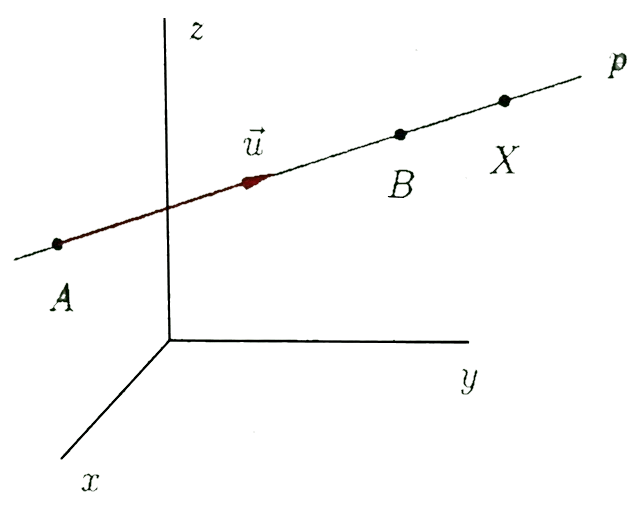
\includegraphics[width=0.5\linewidth]{mai_fig000.png}
    \captionof{figure}{Zadáni přímky. \cite[s.~1]{Musilova2009MA1}
    \label{mai:fig000}}
    \par}        
  Veličinou \(t\), takzvaným \emph{parametrem}, který může nabývat všech reálných hodnot, 
  \(t\in\mathcal{R}\), dokážeme popsat všechny vektory \(\overrightarrow{AX}\), jejichž 
  koncový bod \(X\) leží na přímce \(p\). Naopak, žádné jiné body \(X\) než ty, které leží na 
  přímce \(p\), tuto vlastnost nemají. S označením bodů \(A\), \(X\), resp. vektorů 
  \(\vec{u}\), \(\overrightarrow{AX}\) kartézskými souřadnicemi, resp. složkami
  \begin{align*}
                    A &= (x_A,y_A, z_A), \\ 
                    X &=(x,y,z),         \\
              \vec{u} &= (u_1,u_2,u_3),  \\ 
  \overrightarrow{AX} &= (x - x_A, y - y_1A, z-z_A),
  \end{align*}
  dostáváme \textbf{parametrické vyjádřeni přímky} \(p\) ve tvaru
  \begin{equation}
    p = \left\{(x,y,z)\in\mathcal{R}^3\,|\,
    \begin{matrix}
      x = x_A + tu_1,        \\
      y = y_A + tu_2,        \\
     z = z_A + tu_3,
    \end{matrix}
    \;t\in\mathcal{R}
    \right\}. \label{MAI:eq_M001}
  \end{equation}
\end{example}
\normalsize
      %---------------------------------------------------------------
      Vidíme, že kartézské souřadnice bodu na přímce se vůči souřadnicím bodu \(A\) mění přímo 
      úměrně v závislosti na hodnotě parametru \(t\), tj. závisí na jeho první mocnině. Příslušná 
      závislost se nazývá \textbf{lineární funkcí}.
      
      Obdobně zapíšeme parametrické vyjádření roviny v \(\mathcal{R}^3\):
      %---------------------------------------------------------------
      % !TeX spellcheck = cs_CZ

\begin{example}\label{mai:exam004}
  \textbf{Parametrická vyjádření roviny}:\newline
  Rovina v trojrozměrném prostoru \(\mathcal{R}^3\) je zadána třemi body \(A\), \(B\) a \(C\), 
  které nesmějí ležet v jedné přímce, popřípadě dvěma body \(A\) a \(B\) a vektorem v nerovnoběžným 
  s \(\overrightarrow{AB}\), anebo bodem \(A\) a dvěma nerovnoběžnými směrovými vektory \(\vec{u}\) 
  a \(\vec{u}\) (obr. \ref{MAI:FIG002}). Všechny tyto typy zadání jsou ekvivalentní. Lze volit 
  například \(\vec{u} = \overrightarrow{AB}\), \(\vec{v} = \overrightarrow{AC}\). Je-li \(X\) 
  libovolným bodem roviny \(\varrho\), jsou vektory \(\overrightarrow{AX}\), \(\vec{u}\) a 
  \(\vec{v}\) \textbf{lineárně závislé}. To znamená, že existují taková reálná čísla \(r\) a \(s\), 
  že vektor \(\overrightarrow{AX}\) lze zapsat jako lineární kombinaci

  {\centering
    \captionsetup{type=figure}
    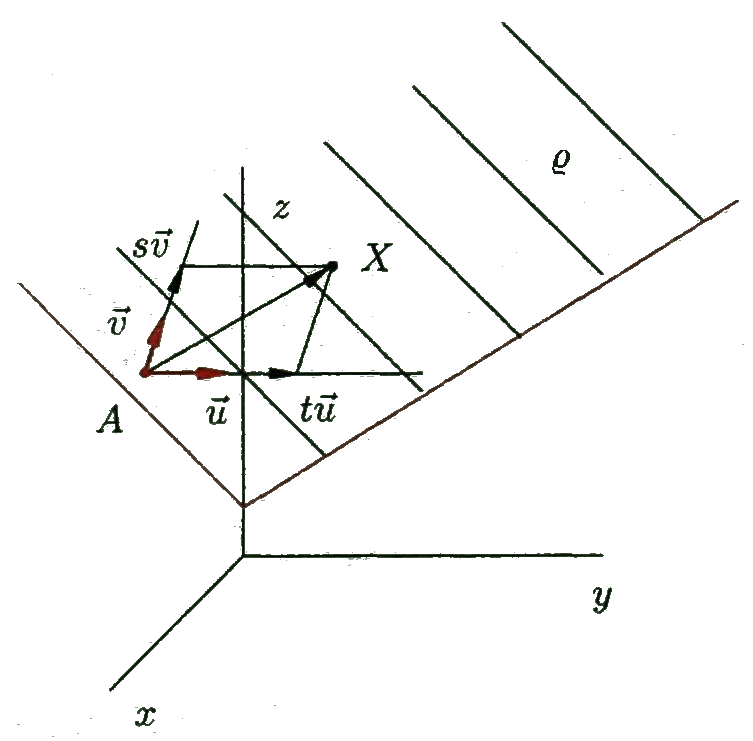
\includegraphics[width=0.5\linewidth]{Musilova_FIG002.png}
    \captionof{figure}{Zadáni roviny. \cite[s.~3]{Musilova2009MA1}}
    \label{MAI:FIG002}
    \par}  
  
\end{example}
  
      %---------------------------------------------------------------
      
    \subsection{Soustavy lineárních rovnic a jejich rychlé řešení}
      Příkladů linearity v přírodě bychom mohli nalézt bezpočet. Vraťme se však k matematice a k 
      problematice uvedené v názvu tohoto odstavce, k soustavám lineárních rovnic. Začněme 
      jednoduchou slovní úlohou ze základní školy:

      %---------------------------------------------------------------
      % !TeX spellcheck = cs_CZ

\begin{example}\label{mai:exam005}
  \textbf{Příklad s ježibabou:}\newline
  Jeníček a Mařenka kradli ježibabě perník. Dohromady snědli 11 perníkových srdíček. Jeníček jich 
  přitom zkonzumoval o 3 více než Mařenka. Otázka je tradiční — kolik srdíček snědl každý z nich?
  Označíme-li \(M\) počet kousků, které snědla Mařenka a \(J\) počet srdíček, na nichž si pochutnal 
  Jenda, můžeme informace zadané v úloze zapsat takto:
    \begin{equation*}
      M + J = 11 \qquad J = M + 3.
    \end{equation*}
  Řešení není problémem, snadno vidíme, že \(M = 4\) a \(J = 7\).
\end{example}
      %---------------------------------------------------------------
      
      O samotné řešení této jednoduché úlohy v tuto chvíli nejde. Pojmenujme si však vztahy, které 
      jsme pro neznámé hodnoty \(M\) a \(J\) ze zadání úlohy dostali. Neznámé vystupují v 
      rovnicích v první mocnině, tedy \emph{lineárně}. Máme \emph{soustavu dvou rovnic} o dvou 
      neznámých \(M\) a \(J\). Úvahu snadno zobecníme: Předpokládejme, že máme neznámé veličiny
      \begin{equation*}
        (x_1, x_2, \ldots, x_n)
      \end{equation*}
      a máme o nich \(m\) informací, které lze zapsat ve tvaru lineárních rovnic (neznámé budou v 
      těchto rovnicích vystupovat v první mocnině),
      \begin{align}
        a_{11}x_1 + a_{12}x_2 + \ldots + a_{1n}x_n &= b_1,     \nonumber           \\
        a_{21}x_1 + a_{22}x_2 + \ldots + a_{2n}x_n &= b_2,     \label{mai:eq002}   \\
        .......................................... &= \ldots   \nonumber           \\
        a_{m1}x_1 + a_{m2}x_2 + \ldots + a_{mn}x_n &= b_m,     \nonumber
      \end{align}
      Soustavu (\ref{mai:eq002}) nazýváme soustavou \(m\) lineárních rovnic o \(n\) neznámých. 
      Označme ji jako \(S\) a pod tímto označením se k ní budeme vracet. Soubory reálných čísel 
      \((a_{ij})\) a \((b_i)\), kde \(1 < i < m\), \(1 \leq j < n\), jsou zadány. Lze je uspořádat 
      do takzvaných \textbf{matic}
      \begin{equation}\label{mai:eq003}
        A =
          \begin{pmatrix}
            a_{11} & a_{12} & \ldots & a_{1n} \\
            a_{21} & a_{22} & \ldots & a_{2n} \\
            \ldots & \ldots & \ldots & \ldots \\
            a_{m1} & a_{m2} & \ldots & a_{mn}          
          \end{pmatrix},
          \overline{B} =
          \begin{pmatrix}
            b_1     \\
            b_2     \\
            \ldots  \\
            b_m 
          \end{pmatrix}
      \end{equation}
      
      Matice \(A\) je typu \(m/n\), má \(m\) řádků a \(n\) sloupců, \(i\) je řádkový index a \(j\) 
      je sloupcový index. Matice \(\overline{B}\) je typu \(m/1\) (\(m\) řádků a jeden sloupec), 
      hovoříme také o sloupcové matici. Soustavu \(S\) můžeme zapsat zkráceně pomocí maticového 
      násobení (podrobněji viz později odstavec \ref{MAI:sec_matice}):
      \begin{equation*}
        A \cdot X = \overline{B}, \qquad \text{nebo}
      \end{equation*}  
      \begin{equation}\label{mai:eq004}
          \begin{pmatrix}
            a_{11} & a_{12} & \ldots & a_{1n} \\
            a_{21} & a_{22} & \ldots & a_{2n} \\
            \ldots & \ldots & \ldots & \ldots \\
            a_{m1} & a_{m2} & \ldots & a_{mn}
          \end{pmatrix}
          \cdot
          \begin{pmatrix}
            x_1     \\
            x_2     \\
            \ldots  \\
            x_m 
         \end{pmatrix}
          =
         \begin{pmatrix}
              b_1     \\
              b_2     \\
              \ldots  \\
              b_m 
            \end{pmatrix}
      \end{equation}
      V tuto chvíli vysvětlíme podstatu maticového násobení jen technicky: Násobit mezi sebou 
      můžeme matici \(A = (a_{ij})\) typu \(m/n\) (levý činitel) a matici \(C = (c_{jk})\) typu 
      \(n/p\) (pravý činitel, činitele nelze zaměňovat). Výsledkem je matice \(D = (d_{ik})\) typu 
      \(m/p\), jejíž prvky se počítají podle předpisu
      \begin{equation}\label{mai:eq005}
        d_{ik} = \sum_{j=1}^{n} a_{ij}\cdot c_{jk}.
      \end{equation}
      
      Z tohoto obecného předpisu vidíme, že levé strany soustavy \(S\) lze interpretovat ve tvaru 
      součinu matice \(A\) typu \(m/n\) s maticí neznámých typu \((n/1)\), výsledkem je matice 
      pravých stran \(\overline{B}\), která je typu \(m/1\). Matice \(A\) se nazývá \textbf{maticí 
      soustavy}. Matice, která vznikne jejím \emph{rozšířením} o sloupec pravých stran, tj.
      \begin{equation}\label{mai:eq006}
        B = (A|\overline{B}) =
        \left(
          \begin{array}{cccc|c}
            a_{11} & a_{12} & \ldots & a_{1n} & b_1    \\
            a_{21} & a_{22} & \ldots & a_{2n} & b_2    \\
            \ldots & \ldots & \ldots & \ldots & \ldots \\
            a_{m1} & a_{m2} & \ldots & a_{mn} & b_m
          \end{array}
        \right)
      \end{equation}
      je pak \textbf{rozšířenou maticí soustavy}. Je-li sloupec pravých stran soustavy tvořen 
      samými nulami, nazývá se soustava \textbf{homogenní}, v opačném případě \textbf{nehomogenní}. 
      Řešením soustavy \(S\) nazýváme každou \(n\)-tici \((x_i, x_2,\ldots, x_n)\), která soustavu 
      \(S\) splňuje. Cílem je najít všechna řešení soustavy \(S\). Abychom řešení nalezli, musíme 
      soustavu upravovat, zjednodušovat. Prováděné úpravy mají vést k jednodušší, avšak 
      ekvivalentní soustavě rovnic, tj. takové, která má naprosto stejný soubor všech řešení jako 
      soustava původní. Takové úpravy nazýváme \textbf{ekvivalentními}. Dvě základní, pomocí nichž 
      lze uskutečnit všechny ostatní, jsou
      \begin{itemize}\addtolength{\itemsep}{-0.5\baselineskip}
        \item vynásobení libovolné, například \(i\)-té, rovnice libovolným \emph{nenulovým} číslem,
        \item přičtení \(i\)-té rovnice vynásobené libovolným číslem k \(l\)-té rovnici.
      \end{itemize}      
      V soustavě lze samozřejmě také měnit pořadí rovnic. Tato úprava je rovněž ekvivalentní. 
      Nevypisujeme ji však zvlášť proto, že ji lze realizovat pomocí vhodně zvolené posloupnosti 
      základních dvou úprav.
      
      Abychom nemuseli soustavu stále opisovat i s neznámými, provádíme obvykle ekvivalentní 
      úpravy jen s maticí \(B = (A|\overline{B})\) (každý řádek této matice představuje jednu 
      rovnici soustavy \(S\)). Může se stát, že soustava má právě \emph{jedno řešení}, jako tomu 
      bylo v  úloze o Mařence a Jeníčkovi. Také nemusí mít \emph{řešení žádné}, jako například 
      soustava \(x + y = 0\), \(x + y = l\) (součet dvou čísel nemůže nabývat současně dvou různých 
      hodnot). A třeba má také řešení \emph{nekonečně mnoho} (řešením soustavy jedné rovnice o dvou 
      neznámých \(x + y = 1\) jsou všechny dvojice tvaru \((x, 1 — x)\), kde \(x\) je libovolné). A 
      může mít soustava \(S\) třeba právě dvě řešení? Prostřednictvím následujícího příkladu 
      ukážeme metodu, která vede velmi rychle k nalezení všech řešení a umožňuje také vyslovit 
      obecné závěry o jejich vlastnostech a počtu. Jedná se o \textbf{Gaussovu eliminační metodu}.
      
 
%--------------------------------------------------------------------------------------------------
  \section{Matice}\label{MAI:sec_matice}
    \begin{definition}\label{def_matice}
      Nechť \(m, n\) jsou přirozená čísla. Jestliže každé uspořádané dvojici \(m,n\). Jestliže každé
      uspořádané dvojici \((m,n)\in \{1,2,\ldots,m\}\times \{1,2,\ldots,m\) přiřadíme prvek
      \(a_{i,j}\in\mathcal{R}\) obdržíme reálnou \href{http://cs.wikipedia.org/wiki/Matice}{matici} 
      typu \(m,n\) nad \(\mathcal{R}\). Čísla jsou indexy, \(i\) je řádkový a \(j\) je sloupcový 
      index.
      
      Matici zapisujeme jako
      \begin{equation}\label{matice_zapis}
        A = \left(a_{ij}\right) =\left(
          \begin{array}{ccc}
            a_{11} & \ldots & a_{1n} \\
            \vdots & \ddots & \vdots \\
            a_{m1} & \ldots & a_{nn}
          \end{array}
        \right)
      \end{equation}
      která má právě \(mn\) prvků \((a_{ij})\) uspořádaných do \(m\) řádků a \(n\) sloupců. Stručně 
      píšeme \(A = (a_{ij})\)
    \end{definition}
  
    \begin{example}
      Matice \(\begin{pmatrix}1&2&3&4\\4&3&2&1\\-1&-1&-1&-1\\-2&-1&0&1\end{pmatrix}\) je čtvercová 
      matice velikosti \(4\times4\). Prvek matice \(a_{23}\) je \(2\).
    \end{example}  
    
    \subsection{Maticová algebra}
      \begin{definition} 
        Součinem matice \(A \in \mathcal{R}_{mn}\) a matice \(B \in \mathcal{R}_{np}\), v uvedeném
        pořadí, je matice \(C \in \mathcal{R}_{mp}\) pro kterou platí:
        \begin{align*}
               C &= AB; \quad C = (cij); \\
               \shortintertext{kde}
          c_{ij} &= \sum_n^{k=1}{a_{ik}b_{kj}};\quad
                     i = 1,\ldots,m; \, j = 1,\ldots,p.
        \end{align*} 
      \end{definition}
      Součin matic \(A\) a \(B\) je definován právě tehdy, když počet sloupců matice \(A\) je roven 
      počtu řádků matice \(B\). Obrázek \ref{LA:fig_LA001a} demonstruje jakým způsobem se 
      dostane prvek, který je ve výsledné matici třeba ve druhém řádku a druhém sloupci, násobením 
      druhého řádku levé matice s druhým sloupcem pravé ze zadaných matic. Stejným způsobem získáme 
      hodnotu prvku \(c_{ij}\) (viz \ref{LA:fig_LA001b}).
%      %----------------------------------
      \begin{figure}[ht!]
        \centering  
        \begin{tabular}{@{}c}
          \subfloat[1. krok]{\label{LA:fig_LA001a}
            %\documentclass[11pt]{standalone}
%  \usepackage{helvet}                        % font
%  \usepackage{xltxtra}                       % fontspec package
%  \usepackage{tikz}  
%  \usetikzlibrary{matrix, arrows}
%  \usepackage{circuitikz}

%\begin{document}

\begin{tikzpicture}

\newcommand{\unit}{0.9cm}
\tikzset{
          node  style    sp/.style={draw,circle,minimum size=\unit},
          node  style    ge/.style={circle,minimum size=\unit}, 
          arrow style   mul/.style={draw,sloped,midway,fill=white}, 
          arrow style  plus/.style={midway,sloped,fill=white},
          yl/.style={},
      }

	\matrix (A) [matrix of math nodes, row sep=-0.5em, column sep=-0.5em, 
               text height=1.5ex, text depth=0.25ex,
			   nodes={node style ge}, left delimiter={(}, right delimiter={)}] at (0,0) {
    a_{11}                          & a_{12}                          & \ldots     & 
    a_{1p}                         \\
    | [node style sp] | {a_{21}}    & | [node style sp] | {a_{22}}    & \ldots     & | [node style 
    sp] | {a_{2p}}   \\
    \vdots                          & \vdots                          & \ddots     & 
    \vdots                         \\
    a_{n1}                          & a_{n2}                          & \ldots     & 
    a_{np}                         \\
  };
    
  \matrix (B) [matrix of math nodes, row sep=-0.5em, column sep=-0.5em, 
               text height=1.5ex, text depth=0.25ex,
			   nodes={node style ge}, left delimiter={(}, right delimiter={)}] at (4.5*\unit,4.5*\unit) {
    b_{11}                          & | [node style sp] | {b_{12}}    & \ldots     & 
    b_{1q}                         \\
    b_{21}                          & | [node style sp] | {b_{22}}    & \ldots     & 
    b_{2q}                         \\
    \vdots                          & \vdots                          & \ddots     & 
    \vdots                         \\
    b_{p1}                          & | [node style sp] | {b_{p2}}    & \ldots     & 
    b_{pq}                         \\
  };
  
  % matrice result
  \matrix (C) [matrix of math nodes, row sep=-0.5em, column sep=-0.5em, 
               text height=1.5ex, text depth=0.25ex,
               nodes={node style ge}, left delimiter={(}, right delimiter={)}] at (4.5*\unit,0) {
    c_{11}                          & c_{12}                            & \ldots     & 
    c_{1q}                       \\
    c_{21}                          & | [node style sp,red] | {c_{22}}  & \ldots     & 
    c_{2q}                       \\
    \vdots                          & \vdots                            & \ddots     & 
    \vdots                       \\
    c_{n1}                          & c_{n2}                            & \ldots     & 
    c_{nq}                       \\
  };

  \draw[blue] (A-2-1.north) -- (C-2-2.north);
  \draw[blue] (A-2-1.south) -- (C-2-2.south);
  \draw[blue] (B-1-2.west)  -- (C-2-2.west);
  \draw[blue] (B-1-2.east)  -- (C-2-2.east);
  \draw[angle 60-angle 60,red](A-2-1) to[in=180,out=90] node[arrow style mul] (x) 
    {\tiny\(a_{21}\times b_{12}\)} (B-1-2);
  \draw[angle 60-angle 60,red](A-2-2) to[in=180,out=90] node[arrow style mul] (y) 
    {\tiny\(a_{22}\times b_{22}\)} (B-2-2);
  \draw[angle 60-angle 60,red](A-2-4) to[in=180,out=90] node[arrow style mul] (z) 
    {\tiny\(a_{2p}\times b_{p2}\)} (B-4-2);
  \draw[red,-angle 60] 
    (x) to node[arrow style plus] {$+$} (y)%
        to node[arrow style plus] {$+\raisebox{.5ex}{\ldots}+$} (z)%
        to (C-2-2.north west);   
  \node [draw, below=5pt] at (A.south) 
    { \tiny\(A\) : \textcolor{red}{\(n\) řádků} \(p\) sloupků};
  \node [draw, above=5pt] at (B.north) 
    { \tiny\(B\) : \(p\) řádků \textcolor{red}{\(q\) sloupků}}; 
  \node [draw, below=5pt] at (C.south) 
    {\tiny\(C=A\times B\) : \textcolor{red}{\(n\) řádků}  \textcolor{red}{\(q\) sloupků}}; 
\end{tikzpicture}
%\end{document}}              \\
          \subfloat[2. krok]{\label{LA:fig_LA001b}
            %\documentclass[11pt]{standalone}
%  \usepackage{helvet}                        % font
%  \usepackage{xltxtra}                       % fontspec package
%  \usepackage{tikz}  
%  \usetikzlibrary{matrix, arrows,decorations}
%  \usepackage{circuitikz}





%\begin{document}
\begin{tikzpicture}

\newcommand{\unit}{0.9 cm}
  \tikzset{
          node  style    sp/.style={draw,circle,minimum size=\unit},
          node  style    ge/.style={circle,minimum size=\unit}, 
          arrow style   mul/.style={draw,sloped,midway,fill=white}, 
          arrow style  plus/.style={midway,sloped,fill=white},
          yl/.style={},
      }

  % defintion of matrices
  \matrix (A) [matrix of math nodes, row sep=-0.9em, column sep=-0.9em, 
               text height=1.5ex, text depth=0.25ex,
			   nodes={node style ge}, left delimiter={(}, right delimiter={)}] at (0,0) {
    a_{11}                       & \ldots & a_{1k}                        & \ldots & 
    a_{1p}                       \\
    \vdots                       & \ddots & \vdots                        & \vdots & 
    \vdots                       \\
    | [node style sp] | {a_{i1}} & \ldots & | [node style sp] | {a_{ik}}  & \ldots & | [node style 
    sp] | {a_{ip}} \\
    \vdots                       & \vdots & \vdots                        & \ddots & 
    \vdots                       \\
    a_{n1}                       & \ldots & a_{nk}                        & \ldots & 
    a_{np}                       \\
  };

  \matrix (B) [matrix of math nodes, row sep=-0.9em, column sep=-0.9em, 
               text height=1.5ex, text depth=0.25ex,
               nodes={node style ge}, 
               left delimiter={(}, right delimiter={)}] at (4.7*\unit,4.0*\unit) {
    b_{11} & \ldots & | [node style sp] | {b_{1j}} & \ldots & b_{1q}  \\
    \vdots & \ddots & \vdots                       & \vdots & \vdots  \\
    b_{k1} & \ldots & | [node style sp] | {b_{kj}} & \ldots & b_{kq}  \\
    \vdots & \vdots & \vdots                       & \ddots & \vdots  \\
    b_{p1} & \ldots & | [node style sp] | {b_{pj}} & \ldots & b_{pq}  \\
  };

  % matrice resultat
  \matrix (C) [matrix of math nodes, row sep=-0.9em, column sep=-0.9em, 
               text height=1.5ex, text depth=0.25ex,
               nodes={node style ge}, left delimiter={(}, right delimiter={)}] at (4.7*\unit,0) {
    c_{11} & \ldots & c_{1j}                           & \ldots & c_{1q} \\
    \vdots & \ddots & \vdots                           & \vdots & \vdots \\
    c_{i1} & \ldots & | [node style sp,red] | {c_{ij}} & \ldots & c_{iq} \\
    \vdots & \vdots & \vdots                           & \ddots & \vdots \\
    c_{n1} & \ldots & c_{nk}                           & \ldots & c_{nq} \\
  };

  % arrows
  \draw[blue] (A-3-1.north) -- (C-3-3.north);
  \draw[blue] (A-3-1.south) -- (C-3-3.south);
  \draw[blue] (B-1-3.west)  -- (C-3-3.west);
  \draw[blue] (B-1-3.east)  -- (C-3-3.east);
  \draw[<->,red](A-3-1) to[in=180,out=90] node[arrow style mul] (x)
    {\tiny\(a_{i1}\times b_{1j}\)} (B-1-3);
  \draw[<->,red](A-3-3) to[in=180,out=90] node[arrow style mul] (y) 
    {\tiny\(a_{ik}\times b_{kj}\)} (B-3-3);
  \draw[<->,red](A-3-5) to[in=180,out=90] node[arrow style mul] (z) 
    {\tiny\(a_{ip}\times b_{pj}\)} (B-5-3);
  \draw[red,->] 
    (x) to node[arrow style plus] {$+\raisebox{.5ex}{\ldots}+$} (y)%
        to node[arrow style plus] {$+\raisebox{.5ex}{\ldots}+$} (z);
      % to (C-3-3.north west);
  \draw[->,red] (z) -- (C-3-3.north west);
  \node [draw, below=5pt] at (A.south) 
    { \tiny\(A\) : \textcolor{red}{\(n\) řádků} \(p\) sloupků};
  \node [draw, above=5pt] at (B.north) 
    { \tiny\(B\) : \(p\) řádků \textcolor{red}{\(q\) sloupků}}; 
  \node [draw, below=5pt] at (C.south) 
    {\tiny\(C=A\times B\) : \textcolor{red}{\(n\) řádků}  \textcolor{red}{\(q\) sloupků}}; 
\end{tikzpicture}
%\end{document}}
        \end{tabular}
        \caption{Postup při maticovém násobení}
      \end{figure}

%--------------------------------------------------------------------------------------------------
    \subsection{Označení prvků matice}
      Prvky matice jsou označeny indexy udávajícími \textbf{řádek} a \textbf{sloupec}, v nichž se 
      prvek nalézá. Prvek v \(i\)-tém řádku a \(j\)-tém sloupci matice \(A\) se obvykle značí 
      \(a_{ij}\). Potom \(i\)-tý řádek matice  obsahuje vodorovnou \(n\)-tici prvků \(a_{i1}, 
      a_{i2}, \ldots,a_{in} \), kde \(i=  1,2,\ldots,m\) a \(j\)-tý sloupec matice obsahuje svislou 
      matici čísel \(a_{1j},a_{2j},\ldots,a_{mj}\), kde \(j = 1,2,\ldots,n\).
  
      V tabulce \ref{LA:tab_basic_matrix} jsou uvedeny nejčastější typy matic, které se v algebře 
      často vyskytují. Jsou to například matice řádkové, sloupcové, diagonální\footnote{Prvky 
      \(a_{ii}\) kde \(i=1,2,\ldots,\min(m,n)\) tvoří hlavní diagonálu. Matice \(\mathbf{D}\) je 
      typu \(m,m\), obecně může mít diagonální matice buď ještě další sloupce, v nichž budou samé 
      nuly, anebo další řádky, v nichž budou opět samé nuly.}, jednotkové\footnote{Jestliže \(m = 
      n\), pak mluvíme o čtvercové matici řádu \(m\).}, nulové, transponované a symetrické.
  
      \begin{table}[!ht]
          \centering
          \renewcommand{\arraystretch}{1.8}   % for the vertical padding
            \begin{tabular}{|l||c@{}|}              
              \hline 
              \textbf{Matice}                    & \textbf{Zápis} \\ \hline\hline
              \ttfamily řádková   \(\mathbf{A}\) &  \(a_1,a_2,\ldots,a_n \)\\
              \ttfamily sloupcová \(\mathbf{B}\) & 
                \(\begin{pmatrix}
                  a_1     \\
                  a_2     \\
                  \vdots  \\
                  a_n
                \end{pmatrix}\)                       \\
              \ttfamily diagonální \(\mathbf{C}\) & 
                \(\begin{pmatrix}
                   a_{11} &    0   & \ldots &   0     \\
                      0   & a_{22} & \ldots &   0     \\
                   \vdots & \vdots & \ddots & \vdots  \\
                      0   &   0    & \ldots & a_{mm}
                \end{pmatrix}\)                       \\
              \ttfamily jednotková \(\mathbf{I}\) &
                \(\begin{pmatrix}
                     1    &    0   & \ldots &   0    \\
                     0    &    1   & \ldots &   0    \\
                   \vdots & \vdots & \ddots & \vdots \\
                      0   &   0    & \ldots & 1
                \end{pmatrix}\)                      \\
              \ttfamily nulová \(\mathbf{0}\) & \((a_{ij}),\quad a_{ij} = 0\,\forall\,i, j\) \\
              \ttfamily transponovaná \(\mathbf{D^T}\) &
                \(\begin{pmatrix}
                  a_{11} & a_{21} & \ldots &  a_{m1}\\
                  a_{12} & a_{22} & \ldots &  a_{m2}\\
                  \vdots & \vdots & \ddots & \vdots \\
                  a_{1n} & a_{2n} & \ldots & a_{mn}
                \end{pmatrix}\)    \\
              \ttfamily symetrická \(\mathbf{S}\) 
              & \((a_{ij}),\quad a_{ij}= a_{ji}\,\forall\,i,j\) \\ \hline
            \end{tabular}
          \caption{Speciální typy matic}\label{LA:tab_basic_matrix}
      \end{table}
    
    
      Matice téhož typu \((m,n)\) nad \(\Re\) budeme značit \(\Re_{m,n}\).
      
      \begin{definition}\label{rovnost_matic}
       (Rovnost matic):  Matice \(\mathbf{A} = \left(a_{ij}\right)\) je rovna matici \(\mathbf{B}=
       \left(b_{kl}\right)\), jsou-li matice stejného typu a stejnolehlé prvky se sobě
       \textbf{rovnají}, tj. \(\mathbf{A} \in \Re_{m,n}, \mathbf{B}\in\Re_{m,n}, a_{ij} = b_{ij}, 
       \forall i\in\lbrace1,2,\ldots,m\rbrace, \forall j\in\lbrace1,2,\ldots,n\rbrace\).
      \end{definition}
      
  %===============================Kapitola: Vektory================================================
  \section{Počítání s vektory}
    \textbf{Vektory} budeme nazývat matice typu \(1/n\) a značit je
    \begin{equation*}
      \vec{u} = (u_1, u_2, \ldots, u_n).
    \end{equation*}
    Takže počítat s nimi již umíme! (V zápisu složek vektoru je vynechán řádkový index. V případě 
    matice s jedním řádkem, takzvané \emph{řádkové matice}, je totiž zbytečný.) Číslům \(u_1\) až 
    \(u_n\) budeme pro tuto chvíli říkat \emph{složky vektoru} \(\vec{u}\). Za chvíli tento pojem 
    ještě upřesníme. Celou řadu pojmů, s nimiž jsme se seznámili při počítání s maticemi, můžeme 
    pro vektory přímo použít. Namísto značení \(\mathcal{M} (1/n)\) budeme pro prostor vektorů 
    používat symbol \((\mathcal{R}^n)\) nebo \(\mathcal{C}^n\) (obvyklý symbol pro množinu 
    uspořádaných \(n\)-tic reálných nebo komplexních čísel).
    
    \subsection{Součiny vektorů}
      Kromě základních operací s vektory, tj. sčítání vektorů a násobení vektoru skalárem, se 
      často používají další operace, které obohacují \emph{strukturu vektorového prostoru}. 
      Zůstaneme u vektorů v trojrozměrném prostoru \(\mathcal{R}^3\) a definujeme si skalární, 
      vektorový a smíšený součin vektorů. Skalární součin vektorů definujeme prostřednictvím 
      geometrické definice jako zobrazení, které uspořádané dvojici vektorů (volných vektorů nebo 
      jejich libovolných umístění) přiřazuje reálný číslo podle předpisu
      
  %===============================Kapitola: Determinanty===========================================
  \section{Determinanty}
    Abychom mohli nadefinovat determinant, budeme muset vědět, jak vypočítat permutaci entice, 
    respektive znaménko permutace.
    \subsection{Permutace}
      \begin{definition}\label{permutace}
        Nechť \(\mathbf{M}\) je libovolná konečná množina. Permutací množiny \(M\) nazýváme 
        zobrazení \(\pi\) množiny \(\mathbf{M}\) na sebe.
      \end{definition}
      
      \begin{example}%(Damlová  Nagy, 1985, str. 34)
        Permutace \(\pi\) množiny \(\mathbf{M}= \lbrace a,b,c,d\rbrace\) je např. zobrazení 
        \(\pi\), definované předpisem:
        \begin{equation}\label{permutace_zadani}
          \pi\left(a\right) = c, \,
          \pi\left(b\right) = d, \,
          \pi\left(c\right) = b, \,
          \pi\left(d\right) = a,
        \end{equation}
        Místo tohoto zápisu se však používá přehlednější zápis ve tvaru matice typu \((2,4)\):
        \begin{equation}\label{LA:eq_perm_exam}
            \begin{pmatrix}
            a & b & c & d \\
            c & d & b & a
            \end{pmatrix}
        \end{equation}
        kde v prvním řádku jsou vypsány všechny prvky množiny \(\mathbf{M}\) (v libovolném pořadí) 
        a ve druhém řádku je pod každým prvkem zapsán jeho obraz v permutaci. Tutéž permutaci však 
        můžeme zapsat ve tvaru matice několika různými způsoby. Například mohou být zapsány takto:
        \begin{equation}
          \begin{array}{cc}
            \begin{pmatrix}
              b & a & c & d \\
              d & c & b & a
            \end{pmatrix},         & 
            \begin{pmatrix}
              d & c & b & a \\
              a & b & d & c
            \end{pmatrix}          \\
            \begin{pmatrix}
              d & c & a & b \\
              a & b & c & d
            \end{pmatrix},         &
            \text{apod.}
          \end{array}
        \end{equation}
      \end{example}

      Zřejmě všechny čtyři uvedené zápisy permutace rov. \ref{LA:eq_perm_exam} ve tvaru matice se 
      liší navzájem pouze pořadím sloupců. Aby bylo možné zapsat každou permutaci množiny 
      \(\mathbf{M}\) ve tvaru rov. \ref{LA:eq_perm_exam} jediným způsobem, je nutné zvolit pevné 
      pořadí prvků množiny \(\mathbf{M}\)  a v zápisu permutace uvádět prvky matice \(\mathbf{M}\)  
      v prvním řádku v tomto pořadí. Avšak známe-li toto pořadí prvků množiny \(\mathbf{M}\), je 
      pak  obvykle zbytečné jej v zápisu permutace uvádět, ale stačí uvést pouze pořadí obrazů, tj. 
      druhý řádek. Zvolíme-li např. v naší množině \(\mathbf{M}\) pevné pořadí prvků \(\lbrace 
      a,b,c,d\rbrace\), pak permutaci rov. \ref{permutace_zadani} zapíšeme jako uspořádanou 
      čtveřici \(\lbrace c,d,b,a\rbrace\).
  
      \begin{definition}\label{def_permutace_ntice}
        Když vytváříme uspořádanou \(n\)-tici navzájem různých prvků \(n\)-prv\-ko\-vé množiny 
        \(\mathbf{M}\), přiřazujeme každému prvku množiny \(\mathbf{M}\) právě jedno přirozené 
        číslo, index příslušného prvku, z množiny prvních \(n\) přirozených čísel.
        \begin{equation}\label{permutace_ntice}
          \pi = \lbrace 1, 2, 3, \ldots, n\rbrace
        \end{equation}
      \end{definition}
  
      Proto každé permutaci uspořádané \(n\)-tice prvků množiny \(\mathbf{M}\) odpovídá jednoznačně 
      permutace příslušných indexů tj. permutace množiny \ref{permutace_ntice} z definice 
      \ref{def_permutace_ntice}. Stačí se tedy omezit při vyšetřování permutací n-prvkové množin 
      na vyšetřování permutací množiny \ref{permutace_ntice}. Permutace \(\pi\) množiny 
      \ref{permutace_ntice} budeme zapisovat jako uspořádané \(n\)-tice \(\left(\pi(1), \pi(2) 
      ,\ldots, \pi(n)\right)\), kde \(\pi(i)\) je číslo z množiny \ref{permutace_ntice}, které 
      permutace \(\pi\) přiřazuje číslu \(i\).

      \begin{example}\label{ex_celk_pocet_permutaci}
        \textbf{Spočítejme celkový počet permutací množiny}. V každé uspořádané \(n\)-tici může být 
        na prvním místě kterákoli z \(n\) cifer, na druhém místě kterákoli ze zbývajících \(n-1\) 
        cifer (kromě té, která je na prvním místě), na  třetím místě každá ze zbývajících \(n-2\) 
        cifer atd. Je tedy celkový počet všech permutací \(n\)-prvkové množiny \(n(n-1)(n-2)\cdot 
        \ldots \cdot2\cdot1\). Toto číslo se zapisuje pomocí symbolu \(n!\) (čti 
        \textbf{n-faktoriál}).
      \end{example}
      
      \begin{definition}\label{def_inv_perm}\textbf{Inverze v permutaci}:
        Inverzí v permutaci \(\left(i_1,i_2,…,i_n \right)\) rozumíme každý výskyt takové dvojice 
        čísel, že větší stojí před menším, tj. vlevo od něj.
      \end{definition}  
   
  %=========================== Kapitola: Vlastní čísla a vlastní vektory ==========================
  \section{Vlastní čísla a vlastní vektory}
    \subsection{Motivace} 
      \textbf{Poznámka}: Je-li \(\mathcal{A} : \mathcal{V} \rightarrow \mathcal{V}\) lineární 
      zobrazení z prostoru \(\mathcal{V}\) do prostoru \(\mathcal{V}\) (nikdy se takové zobrazení 
      nazývá lineárním operátorem), pak je přirozeným požadavkem najít takovou bázi prostoru 
      \(\mathcal{V}\), že je matice zobrazení $\mathbf{A}$ v této bázi co nejjednodušší, např. má 
      následující strukturu
      \begin{equation*}
         \mathbf{A}=
           \left(\begin{array}{ccccc}
             \boxed{A_1}       &             &       &       & 0   \\
                 & \boxed{A_2} &             &       &             \\
                 &             & \boxed{A_3} &       &             \\
                 &             &             &\ddots &             \\
              0  &             &             &       & \boxed{A_k}
            \end{array}
           \right),
     \end{equation*}
     kde \(A_k\) jsou čtvercové matice malého řádu (nejlépe \(1\) nebo \(2\)) a ostatní prvky 
     matice jsou nulové. Problém najít bázi, aby v ní matice zobrazení měla diagonální tvar (kde 
     \(A_k\) jsou skaláry), vede k pojmu vlastní číslo a vlastní vektor matice.

      \begin{definition} 
        Nechť \(\mathbf{A}\in \mathcal{C}^{n,n}\) (matice je čtvercová řádu \(n\)).
        \begin{equation}
          \mathbf{A} = (a_{ij}) =
            \begin{pmatrix}
              a_{11} & a_{12} & \ldots & a_{1n} \\
              a_{21} & a_{22} & \ldots & a_{2n} \\
              \vdots & \vdots & \ddots & \vdots \\
              a_{n1} & a_{n2} & \ldots & a_{nn}
            \end{pmatrix}
        \end{equation}

        Jestliže platí
        \begin{equation}\label{eq:vl_number}
          \mathbf{Au} = \lambda\mathbf{u}
        \end{equation}
        pro jisté komplexní číslo \(\lambda\in\mathcal{C}\)  a jistý nenulový vektor 
        \(x\in\mathcal{C}^n, \mathbf{u}\neq\Theta\), potom číslo \(\lambda\) nazýváme 
        \textbf{vlastním číslem} matice \(\mathbf{A}\) a vektor \(\mathbf{u}\) \textbf{vlastním 
        vektorem} příslušným k tomuto vlastnímu číslu. Množinu všech vlastních čísel nazýváme 
        \textbf{spektrem matice} \(\mathbf{A}\). Pokud rov. \ref{eq:vl_number} rozepíšeme, dostaneme
        \begin{equation}
          \begin{pmatrix}
            a_{11} & a_{12} & \ldots & a_{1n} \\
            a_{21} & a_{22} & \ldots & a_{2n} \\
            \vdots & \vdots & \ddots & \vdots \\
            a_{n1} & a_{n2} & \ldots & a_{nn}
          \end{pmatrix}   \cdot
          \begin{pmatrix}
            u_{1} \\  u_{2} \\ \vdots \\  u_{n} \\
          \end{pmatrix}    =\lambda\cdot
          \begin{pmatrix}
            u_{1} \\ u_{2} \\ \vdots \\ u_{n} \\
          \end{pmatrix}
        \end{equation}
        můžeme ji rovněž psát ve tvaru
        \begin{equation*}
            \begin{pmatrix}
            \setlength{\arraycolsep}{3pt}
              a_{11} -\lambda & a_{12}           & \ldots & a_{1n} \\
              a_{21}          & a_{22} -\lambda  & \ldots & a_{2n} \\
              \vdots          & \vdots           & \ddots & \vdots \\
              a_{n1}          & a_{n2}           & \ldots & a_{nn}-\lambda
            \end{pmatrix} \cdot
          \begin{pmatrix}
            u_{1} \\ u_{2} \\ \vdots \\ u_{n} \\
          \end{pmatrix}  =
          \begin{pmatrix}
              0 \\ 0 \\ \vdots \\ 0 \\
            \end{pmatrix}
        \end{equation*}
      \end{definition}

       Tato soustava rov. je \textbf{homogenní} a stručně ji můžeme zapsat
      \begin{equation}\label{vv_hom_zapis}
        \left(\mathbf{A} - \lambda\mathbf{I}\right) = \mathbf{0}
      \end{equation}
      Homogenní soustava má \emph{netriviální řešení}, právě když je determinant matice soustavy 
      roven  nule, tj. v případě soustavy rov. rov. \ref{vv_hom_zapis} platí
      \begin{equation}\label{vv_hom_reseni}
        |\mathbf{A} - \lambda\mathbf{I}| = \mathbf{0}
      \end{equation}
      Determinant \(A(\lambda)=|\mathbf{A} - \lambda \mathbf{I}|\) nazýváme 
      \textbf{charakteristický polynom} matice \(\mathbf{A}\) - jedná se o polynom stupně \(n\) v 
      proměnné \(\lambda\), který má v oboru komplexních čísel \(n\) kořenů. Rovnici 
      \(A(\lambda)=0\) nazýváme \textbf{charakteristická rovnice matice \(\mathbf{A}\)} - jejími 
      kořeny jsou \textbf{charakteristické hodnoty} (resp. \textbf{vlastní čísla}) 
      \textbf{matice} \(\mathbf{A}\).
            
      \begin{note}
        U vlastních čísel studium pouze reálných matic ztrácí smysl, protože i 
        reálná matice může mít komplexní vlastní čísla. Proto se uvažuje obecná komplexní matice.
      \end{note}
      
      \begin{note}
        Podmínka existence nenulového vektoru \(\mathbf{u} = \Theta\) v definici 
        vlastního čísla je nezbytná: kdyby bylo připuštěno i \(\mathbf{u} = \emptyset\), potom by 
        každé komplexní číslo bylo vlastním číslem a definice by ztratila smysl.
      \end{note}
      
      \begin{note}
        Odpovídá-li matice \(\mathbf{A}\) matici nějakého zobrazení \(\mathcal{A}\), pak každý 
        nenulový vektor z jádra zobrazení \(\ker\mathcal{A}\) je vlastním vektorem příslušným 
        vlastnímu číslu \(\lambda\). Je-li \(\ker\mathcal{A} = \{\Theta\}\) 
        (je-li matice \(\mathbf{A}\) regulární), pak \(\Theta\) není vlastním číslem matice 
        \(\mathbf{A}\).
      \end{note}

      %---------------------------------------------------------------
        % !TeX spellcheck = cs_CZ

\begin{example}\label{mai:exam012}
  Je-li \(\mathbf{P}\) matice ortogonální projekce v prostoru \(\mathcal{R}^3\) na nějaký 
  podprostor \(\mathcal{U}\) (\(\mathcal{U}\) je tedy buď rovina nebo přímka procházející 
  počátkem), pak pro každý vektor \(\mathbf{u}\in\mathcal{U}\) platí \(\mathbf{Pu} = 
  \mathbf{u}\), všechny vektory z \(\mathcal{U}\) (s výjimkou nulového vektoru \(\Theta\)) 
  jsou vlastními vektory matice $\mathbf{P}$ příslušné vlastnímu číslu \(\lambda\). Prostor 
  \(\mathrm{U}^\bot\) je roven jádru projekce (nulovému prostoru matice \(\mathbf{P}\)), 
  a tedy každý vektor z ortogonálního doplňku \(\mathcal{U}\) (s výjimkou \(\Theta\)) je 
  vlastním vektorem příslušným k vlastnímu číslu \(0\).

  {\centering
    \captionsetup{type=figure}
    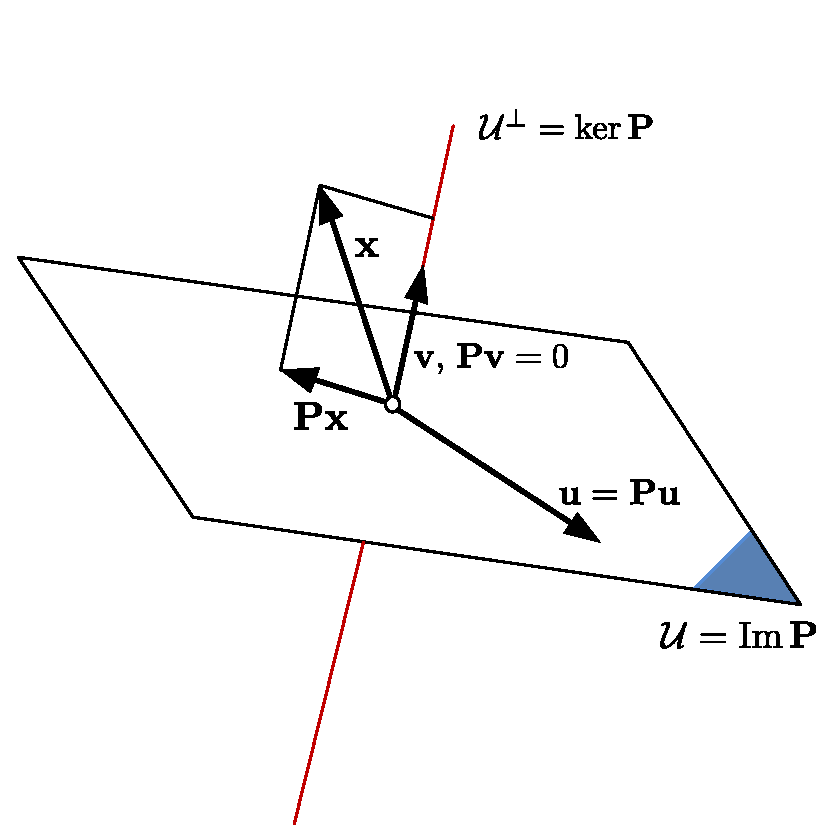
\includegraphics[width=0.7\linewidth]{MAI016.pdf}
    \captionof{figure}{K příkladu \ref{mai:exam012}}
    \label{MAI:FIG016}
    \par}        
\end{example}
      %---------------------------------------------------------------

      %---------------------------------------------------------------
        % !TeX spellcheck = cs_CZ


\begin{example}\label{mai:exam013}
  Určete spektrum matice a její spektrální poloměr následující matice
    \begin{equation*}\label{pr:spektrum_matice}
      \mathbf{A} =
        \begin{pmatrix}
          2  &  2    & 0 \\
         -3  & -3    & 5 \\
          0  & -0.25 & 2
        \end{pmatrix}
    \end{equation*}
  \textbf{Řešení}: Spektrum matice je množina všech jejích vlastních čísel. Spektrální poloměr 
  je maximum z absolutních hodnot vlastních čísel. Vlastní čísla určíme z charakteristické
  rovnice \(\det(\mathbf{A}-\lambda \mathbf{I})=0\).
    \begin{equation*}
      \textbf{A} - \lambda\textbf{I}=
        \begin{pmatrix}
          2-\lambda  &  2          & 0 \\
         -3          & -3-\lambda  & 5 \\
          0          & -0.25       & 2-\lambda
       \end{pmatrix}
    \end{equation*}
    \begin{align}
      \det(\mathbf{A}-\lambda \mathbf{I})                    &= 0           \nonumber\\
      (2-\lambda)
        \begin{pmatrix}
          -3-\lambda  &  5\\
             -0.25    &  2 - \lambda
        \end{pmatrix} -2\cdot
        \begin{pmatrix}
          -3       &  5\\
           0       &  2 - \lambda
        \end{pmatrix}                                        &= 0           \nonumber\\
      (2-\lambda)^2(-3-\lambda)+1.25(2-\lambda)+6(2-\lambda) &= 0           \nonumber\\
      (2-\lambda)[(2-\lambda)(-3-\lambda)+1.25+6]            &= 0           \nonumber\\
      (2-\lambda)(\lambda^2+\lambda+1.25)                    &= 0           \nonumber
    \end{align}
    \begin{equation*}
      \lambda_1 = 2, \quad\lambda_2 = -0.5+i, \quad\lambda_3=-0.5-i
    \end{equation*}
    \begin{itemize}
      \item Spektrum matice \(\mathbf{A}\) je \(\sigma(\mathbf{A})=\{2,-0.5+i,-0.5-i\}\).
      \item Spektrální poloměr \(\rho(\mathbf{A})=\max_i|\lambda_i|=2\).
    \end{itemize}

%    \attachfile[icon=Paperclip, description=Matlab Determine the spectrum of a matrix 
%      and its spectral radius]{../SRC/MAI/matlab/LA001.m}

\end{example}
      %---------------------------------------------------------------

      %---------------------------------------------------------------
        % !TeX spellcheck = cs_CZ
\begin{example}\label{mai:exam014}
  Určete vlastní čísla a vlastní vektory matice \(\mathbf{B} = \mathbf{A}^2 - 4\mathbf{A} + 
  9\mathbf{A}^{-1} - \mathbf{I}\), kde \(\mathbf{A}\) je matice \(\mathbf{A}= 
  \begin{pmatrix}1&0.5\\3.5&4\end{pmatrix}\).

  \textbf{Řešení}: (z předchozího příkladu víme, že \(\lambda_1=4.5, \lambda_2=0.5\)) a
   \(\mathbf{I}\) jednotková matice. Označme symbolem \(\lambda\) vlastní číslo matice 
   \(\mathbf{A}\) a nechť \(\mathbf{x}\) je příslušný vlastní vektor. Pak platí:
   \begin{itemize}
     \item Matice \(\mathbf{A}^2\) má vlastní čísla rovna \(\lambda^2\).
     \item Matice \(4\mathbf{A}\) má vlastní čísla rovna \(4\lambda\).
     \item Matice \(9\mathbf{A}^{-1}\) má vlastní čísla rovna \(\frac{9}{\lambda}\).
   \end{itemize}
   Matice \(\mathbf{B}=\mathbf{A}^2-4\mathbf{A}+9\mathbf{A}^{-1}-\mathbf{I}\) má vlastní čísla 
   ve tvaru  \(\lambda^2-4\lambda+\frac{9}{\lambda}-1\), vlastní vektory jsou stejné jako 
   vlastní vektory odpovídající vlastním číslům matice \(\mathbf{A}\). Tedy:
   \begin{equation*}
       \sigma(B)=\{4.5^2-4\cdot4.5+\frac{9}{4.5}-1,\quad
       0.5^2-4\cdot0.5+\frac{9}{0.5}-1\}=\{3.25, 15.25\}
   \end{equation*}
\end{example}
      %---------------------------------------------------------------


      %---------------------------------------------------------------
       % !TeX spellcheck = cs_CZ

\begin{example}\label{mai:exam002}
  Určete vlastní čísla a odpovídající vlastní vektory následují\-cích matic:
  \begin{equation*}
    \mathbf{A}=
      \begin{pmatrix}
        1   & 0.5\\
        3.5 & 4
      \end{pmatrix}, \quad
    \mathbf{B}=
      \begin{pmatrix}
        3   & -1 \\
        2.5 &  4 
      \end{pmatrix}
  \end{equation*}
  \textbf{Řešení}: Vlastní čísla určíme z charakteristické rovnice: \(\det(\mathbf{A} - 
  \lambda\mathbf{I}) = 0\). Vlastní vektory \(\mathbf{x_i}\) odpovídající vlastním číslům 
  \(\lambda_i\), jsou řešením homogenní soustavy rovnic \((\mathbf{A} - 
  \lambda_i\mathbf{I})\mathbf{x_i} = 0\).
  \begin{itemize}
    \item Vlastní čísla matice \textbf{A}:
      \begin{equation*}
           \textbf{A} - \lambda\textbf{I} =
             \begin{pmatrix}
                1-\lambda  &  0.5          \\
               -3.5        &  4-\lambda
             \end{pmatrix}
      \end{equation*}
      \begin{align*}
         \det(\mathbf{A}-\lambda\mathbf{I}) &= 0 \\
         (1-\lambda)(4-\lambda)-\frac{7}{4} &= 0 \\
         \lambda^2-5\lambda+\frac{9}{4}     &= 0
      \end{align*}
      \begin{equation*}
         \lambda_1 = 4.5,\quad \lambda_2 = 0.5
      \end{equation*}
  \end{itemize}

    \begin{itemize}
      \item Vlastní čísla matice \textbf{B}:
        \begin{equation*}
             \textbf{B} - \lambda\textbf{I}=
               \begin{pmatrix}
                 3-\lambda  & -1             \\
                 2.5        &  4-\lambda
               \end{pmatrix}
        \end{equation*}
        \begin{align*}
           \det(\mathbf{B}-\lambda\mathbf{I}) &= 0 \\
           (3-\lambda)(4-\lambda)+\frac{5}{2} &= 0 \\
           \lambda^2-7\lambda+\frac{29}{2}    &= 0
        \end{align*}
        \begin{equation*}
           \lambda_1 = \frac{7+3i}{2},\quad \lambda_2 = \frac{7-3i}{2}
        \end{equation*}
    \end{itemize}
  % matice A
  Vlastní vektor matice \(\mathbf{A}\) pro \(\lambda_1=4.5: (\mathbf{A} - 
  \lambda_1\mathbf{I})\mathbf{x_1} = 0 \Rightarrow\)
  \begin{align*}
    \begin{pmatrix}
       1  -4.5  &  0.5     \\
      -3.5      &  4-4.5
    \end{pmatrix}
    &\sim
    \begin{pmatrix}
      -3.5  &  0.5         \\
      -3.5  & -0.5
    \end{pmatrix}          \\
    \Rightarrow\mathbf{x_1} &=
    \begin{pmatrix}
      1 \\ 7
    \end{pmatrix}
    \, r, r\in\mathbb{R}, r\neq0
  \end{align*}
  Vlastní vektor matice \(\mathbf{A}\) pro \(\lambda_2=0.5: (\mathbf{A} - 
  \lambda_1\mathbf{I})\mathbf{x_2}=0 \Rightarrow\)
  \begin{align*}
    \begin{pmatrix}
       1  -0.5  &  0.5   \\
      -3.5      &  4-0.5
    \end{pmatrix}
    &\sim
    \begin{pmatrix}
       0.5  &  0.5       \\
       3.5  &  3.5
    \end{pmatrix}        \\
    \Rightarrow\mathbf{x_2} &=
    \begin{pmatrix}
      -1 \\ 1
    \end{pmatrix}
    \, r, r\in\mathbb{R}, r\neq0
  \end{align*}
  % matice B
  Vlastní vektor matice \(\mathbf{A}\) pro \(\lambda_1=\frac{7+3i}{2}: (\mathbf{B} - 
  \lambda_1\mathbf{I})\mathbf{x_1}=0 \Rightarrow\)
  \begin{align*}
    \begin{pmatrix}
       3 - \frac{7+3i}{2}            & -1                                     \\
       \frac{5}{2}                   &  4 - \frac{7+3i}{2}
    \end{pmatrix}
    \sim
    \begin{pmatrix}
      -\frac{1}{2}-\frac{3}{2}i      &  -1                                     \\
      \frac{5}{2}                    & \frac{1}{2}-\frac{3}{2}i
    \end{pmatrix}
    \sim \\
    \begin{pmatrix}
      -\frac{10}{4}                  &-\left(\frac{1}{2} -\frac{3}{2}i\right)  \\
      \frac{5}{2}                    & \frac{1}{2}-\frac{3}{2}i
    \end{pmatrix}
    \sim
    \begin{pmatrix}
      -5                           &-\left(1-3i\right)                         \\
       5                           & \left(1-3i\right)
    \end{pmatrix}
    \rightarrow \\
    \mathbf{x_1}=
    \begin{pmatrix}
      -1+3i \\ 5
    \end{pmatrix}
    \, r, r\in\mathbb{C}, r\neq0
  \end{align*}
  Vlastní vektor matice \(\mathbf{B}\) pro \(\lambda_2=\frac{7-3i}{2}: (\mathbf{B} - 
  \lambda_1\mathbf{I})\mathbf{x_2}=0 \Rightarrow\)
  \begin{align*}
    \begin{pmatrix}
       3  - \frac{7-3i}{2}       &  -1                                     \\
      \frac{5}{2}                &  4 - \frac{7-3i}{2}
    \end{pmatrix}
    \sim
    \begin{pmatrix}
      -\frac{1}{2}+\frac{3}{2}i  &  -1                                     \\
      \frac{5}{2}                & \frac{1}{2}+\frac{3}{2}i
    \end{pmatrix}
    \\sim \\
    \begin{pmatrix}
      -\frac{10}{4}              &-\left(\frac{1}{2} +\frac{3}{2}i\right)  \\
      \frac{5}{2}                & \quad\frac{1}{2}+\frac{3}{2}i
    \end{pmatrix}
    \sim
    \begin{pmatrix}
      -5                         &-\left(1+3i\right)                       \\
       5                         & \quad\left(1+3i\right)
    \end{pmatrix}
    \rightarrow\\
    \mathbf{x_2}=
    \begin{pmatrix}
      -1-3i \\ 5
    \end{pmatrix}
    \, r, r\in\mathbb{C}, r\neq0
  \end{align*}
\end{example}
%---------------------------------------------------------------
\lstinputlisting{../src/MAI/matlab/LA001.m}
\begin{lstlisting}[caption=Výpis programu pro ověření výpočtu vlastních čísel matic programem
  Matlab.]
\end{lstlisting}
%---------------------------------------------------------------
      %---------------------------------------------------------------

  %====================== Kapitola: Polynomy ======================================================
  \section{Polynomy}
      \begin{definition}\label{def_rov_poly}\textbf{Rovnost dvou polynomů}:
        Řekneme, že dva polynomy \(f(x)=a_nx^n+a^{(n-1)}x_{(n-1)}+\ldots+a_1+a_0\) a
        \(g(x)=b_mx^m+b^{(m-1)}x_{(m-1)}+\ldots+b_1+b_0\) stupňů \(n\) a \(m\) se sobě 
        \textbf{rovnají} právě tehdy, když \(m=n\) a \(a_0=b_0\), \(a_1=b_1\), 
        \(a_{(n-1)}=b_{(m-1)}\), \(a_n=b_m\). V tomto případě také říkáme, že mnohočleny \(f(x)\) a 
        \(g(x)\) jsou \textbf{totožné}.
      \end{definition}
      \begin{lemma}\label{la:eq_eqv_poly}
        Jestliže mnohočleny \(f(x)\) a \(g(x)\) jsou dva polynomy stupně \(n\)-tého a jestliže pro 
        \(n+1\) různých reálných nebo komplexních čísel \(x\) platí \(f(x)=g(x)\), potom jsou 
        polynomy \textbf{totožné}.
      \end{lemma}
      
    \subsection{Rozklad ryze racionální funkce na parci\-ální zlomky}

      %---------------------------------------------------------------
       % !TeX spellcheck = cs_CZ
\begin{example}\label{mai:exam015}
  Rozložte na parciální zlomky lomenou racionální funkci \((x):y=\frac{7x+8}{x^2+x-2}\).
  \newline\textbf{Řešení:} Nejprve vypočteme nulové body jmenovatele:
  \begin{align*} 
     x^2+px+q &=(x-u)(x-v) = x^2-(u+v)x+uv            \\
              &\rightarrow p=-(u+v),\quad q=uv
  \end{align*}
  Kořenové činitele  \(x^2+x-2\rightarrow x_1=1, x_2=-2\) zvolíme za jmenovatele parciálních
  zlomků a rozklad hledáme ve tvaru \(\frac{7x+8}{x^2+x-2}=\frac{A}{x-1}+\frac{B}{x+2}\)
  kde \(A\), \(B\) jsou neznámé konstanty. Tyto konstanty určíme tak, aby rozklad platil pro 
  každé \(x\in\mathcal{R}-\{1,-2\}\). Po jednoduché úpravě dostaneme rovnost dvou polynomů
  \(7x+8=(A+B)x+2A-B\). Podle \ref{la:eq_eqv_poly} se musí rovnat koeficienty u \(x\) a absolutní 
  členy obou stran poslední rovnice \(\Rightarrow\) dostaneme soustavu rovnic pro určení \(A\) a 
  \(B\) ve tvaru:
  \begin{align}
    % \nonumber to remove numbering (before each equation)
    7 &= A+B  \nonumber \\ 
    8 &= 2A+B \label{la:eq_parc_example}   
  \end{align}
  dostáváme \(A=5,\quad B=2\). Postup, který jsme užili, nazýváme \textbf{Metodou neurčitých 
  koeficientů}.
  
  Pro určení koeficientů \(A\), \(B\) se užívají také jiné postupy, např. dosazování
  kořenů jmenovatele, která je výhodná zejména v případech, kdy jmenovatel lomené racionální
  funkce má jednoduché kořeny. Postupujeme tak, že rov. \ref{la:eq_parc_example} násobíme
  součinem kořenových činitelů \((x-1)(x+2)=x^2+x-2\) a dostaneme rovnici 
  \(7x+8=A(x+2)+B(x-1)\) pro určení koeficientů \(A\), \(B\) dosazováním kořenů.
    \begin{align*}
      % \nonumber to remove numbering (before each equation)
      x=-2 &\rightarrow       -14+8=B(-2-1)      \rightarrow B=2\\
      x=+1 &\rightarrow  \,\,\,+7+8=A(1+2)\quad  \rightarrow A=5
    \end{align*}
\end{example}
      %---------------------------------------------------------------
      
  %==================== Kapitola: Vektorové prostory ===============================================
  \section{Vektorové prostory se skalárním součinem}
    \subsection{Ortogonální doplňky}
      Nechť \(U\) je podprostor vektorového prostoru \(V\). Ortogonální doplněk $U^\bot$ obsahuje 
      všechny vektory, které jsou kolmé ke každému vektoru z \(U\), neboli \(\forall\vec{v}\in 
      U^\bot\quad \forall\vec{u}\in U\quad \vec{u}\bot\vec{v}\) což lze vyjádřit pomocí skalárního 
      součinu \(\vec{u}\cdot\vec{v} = 0\)
  
      Ortogonální doplněk \(U^\bot\) k podprostoru \(U = \langle\vec{u}_1,\ldots,\vec{u}_k\rangle\) 
      tedy hledáme jako řešení homogenní soustavy rovnic
      \begin{equation*}
        \left(
          \begin{array}{c|c}
             \vec{u}_1  &   0      \\
             \cdots     &  \vdots  \\
             \vec{u}_k  &   0
          \end{array}
        \right),
      \end{equation*}
      nuly na pravé straně při výpočtu zpravidla vynecháváme. Připomeňme také vztah
      \begin{equation}\label{LA:eq_dim_doplnek}
         \dim U + \dim U^\bot = \dim V
      \end{equation}

      %---------------------------------------------------------------
        % !TeX spellcheck = cs_CZ
% Musilova2009MA1

\begin{example}\label{mai:exam011}
  Zjistěte ortogonální doplněk \(\langle(1,-3,2),(2,1,5)\rangle\bot^.\). (Zdroj:
  \cite[s.~3]{MosnaMA3})
  \newline\textbf{Řešení}:
  Hledáme vektor \((x, y, z)\), jehož skalární součin je se zadanými vektory roven nule. Budeme 
  tedy řešit (úpravou na Gaussův tvar pomocí elementárních úprav) homogenní soustavu rovnic
  zadanou maticí
  \begin{equation*}
     \left(
       \begin{array}{ccc|c}
          1  &  -3  & 2 & 0 \\
          2  &   1  & 5 & 0
       \end{array}
     \right)\sim
     \left(
       \begin{array}{ccc|c}
          1  &  -3  & 2 & 0 \\
          0  &   7  & 1 & 0
       \end{array}
     \right)\
  \end{equation*}
  Odtud dostáváme \(z = \alpha\), \(7y + z = 0\) \(\Rightarrow\) \(y = -\frac{1}{7}\alpha\), \(x
  +\frac{3}{7}\alpha + 2\alpha = 0\) \(\Rightarrow\) \(x = -\frac{17}{7}\) neboli 
  \begin{equation*}
  (x, y, z) =\alpha\left(-\frac{17}{7}, -\frac{1}{7}, 1\right) = \alpha(17, 1, -7)
  \end{equation*}

  V dalších příkladech budeme nuly na pravé straně soustavy vynechávat a upravovat na
  výhodnější tvar
  \begin{align*}
       \begin{pmatrix}
          1  &  -3  & 2  \\
          2  &   1  & 5
       \end{pmatrix}
       & \sim
       \begin{pmatrix}
          1  &  -3  & 2 \\
          0  &   7  & 1
       \end{pmatrix}
       \sim                         \\
       \begin{pmatrix}
          1  &   0  & \frac{17}{7}  \\
          0  &   7  & 1
       \end{pmatrix}
       & \sim
       \begin{pmatrix}
          7  &   0  & 17 \\
          0  &   7  & 1
       \end{pmatrix}.
  \end{align*}
  Odtud již snadno zjistíme, že vektor \((x, 1, -7)\) jistě vyhovuje druhé rovnici. Dosadíme-li ho 
  do první rovnice, dostaneme \(7x + 17\cdot(-7) = 0\) a \(x = 17\).

  Hledaný ortogonální doplněk je tedy lineární obal $$\langle(17, 1, -7)\rangle^\bot.$$
  
    {\centering
     \captionsetup{type=figure}
    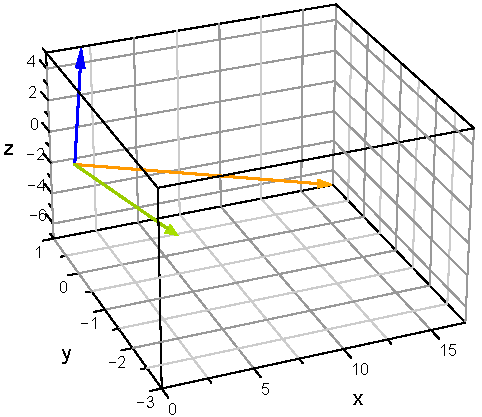
\includegraphics[width=0.8\linewidth]{ort_doplnek_exam01.pdf}
    \captionof{figure}[Ortogonální doplněk]{Vizualizace vektorového prostoru a jeho    
             ortogonálního doplňku pomocí sw MatLab - MuPAD příkazem:\newline
             \texttt{plot(plot::Arrow3d([1,-3,2]), plot::Arrow3d([2,1,5]), 
             plot::Arrow3d([17,1,-7]))}}
    \label{LA:fig_ort01}
    \par}
\end{example}

      %---------------------------------------------------------------
  
      Výsledek předchozího příkladu \ref{mai:exam011} lze interpretovat tak, že jsme našli všechny 
      vektory, které jsou kolmé na rovinu určenou vektory ze zadání. Rovina je útvar       
      dvojrozměrný a protože prostor všech vektorů je trojrozměrný, musí nutně mít podprostor 
      ortogonálních vektorů ve shodě se vztahem \ref{LA:eq_dim_doplnek} pouze jednu dimenzi. Vše 
      je dobře patrné z obr. \ref{LA:fig_ort01}

} % tikzset
%---------------------------------------------------------------------------------------------------
\printbibliography[title={Seznam literatury}, heading=subbibliography]
\addcontentsline{toc}{section}{Seznam literatury}
   %     Differential calculus
%--------------------------------------------------------------------------------------------------
% file Diff_calc.tex
%--------------------------------------------------------------------------------------------------
\chapter{Limita a spojitost funkce}\label{MA1:chap_Limita}
\minitoc
\newpage
  %================Podkapitola: Reálná funkce =====================================================
  \section{Reálná funkce}
    %----------------------------------------------------------------------------------------------
    \subsection{Pojem funkce}
    %----------------------------------------------------------------------------------------------
    \subsection{Graf funkce. Různé způsoby zadání funkce}
      Každé funkci můžeme přiřadit její graf. 
      \textbf{Grafem funkce} $f:A\rightarrow\realset,\ A\subset\realset$, rozumíme množinu všech bodů 
      euklidovské roviny, jejíž souřadnice $x$, $y$ v dané kartézské soustavě souřadnic vyhovuje rovnice 
      \begin{equation}\label{MAI:eq_graf04}
        y=f(x). 
      \end{equation}  
      
      Grafem funkce může v jednodušších případech posloužit jako prostředek k získání názorné       
      \textquotedblleft představy\textquotedblright. Grafy některých funkcí jsou \textquotedblleft 
      křivky\textquotedblright\, (intuitivním smyslu tohoto slova). Avšak u některých funkcí názorná 
      představa grafu selhává. Vezmeme-li např. Dirichletovu funkci z odst. **, snadno zjistíme, že její graf 
      nemůžeme sestrojit (byly by to \textquotedblleft dvě rovnoběžné přímky $y=0$ a $y=1$ s nekonečným 
      množstvím mezer\textquotedblright)
      
      Zadat funkci znamená udat její definiční obor a \textquotedblleft zobrazovací předpis 
      \textquotedblright, tj pravidlo (formulované slovně či v používaném matematickém jazyku), 
      podle něhož můžeme jednoznačným způsobem rozhodnout, jaká funkční hodnota odpovídá libovolně 
      zvolenému číslu z definičního oboru. Definičním oborem bývá často interval nebo sjednocení 
      intervalů. Není-li definiční obor udán, rozumíme jím množinu všech reálných čísel, pro něž je 
      příslušný předpis definován. Tuto množinu nazýváme \textbf{přirozeným (též maximálním) 
      definičním oborem funkce}. Je to tzv. \emph{existenční obor} výrazu, jímž je funkce definována 
      \cite[s.~84]{Brabec1989}.
      
      Například funkce $f: \realset\rightarrow\realset,\ f(x)=x^2$, můžeme vyjádřit bez udání definičního  
      oboru 
      $\realset$ vztahem 
      \begin{equation*}
        f: y=x^2,
      \end{equation*}
      neboť předpis $y=x^2$ má smysl pro každé reálné číslo $x$. Avšak u funkce 
      $g:\langle0,1\rangle\rightarrow\realset,\ g(x)=x^2,$ je nutné v zápisu funkce definiční obor 
      $\langle0,1\rangle$ uvést, píšeme tedy   
      \begin{equation*}
        g: y=x^2, \quad x\in\langle0,1\rangle.
      \end{equation*}
      Zobrazovací předpis, kterým je funkce zadána, může být rozmanitý. Nejčastěji a pro účely matematické 
      analýzy nejvhodnější je \emph{analytické zadání vzorcem}, tj. rovnicí tvaru $y=f(x)$ nebo několika 
      takovými rovnicemi platnými pro různé části definičního oboru. Přitom v rovnici $y=f(x)$ je na pravé 
      straně nějaký správně definovaný výraz obsahující nejvýše poměnnou $x$ a nabývající jednoznačné hodnoty 
      pro danou hodnotu proměnné $x$.

      \begin{example}\label{MAI:exam01} 
        Vzorcem $f(x)=\sqrt{1-x}$ je dána funkce, jejímž přirozeným oborem je interval $(-\infty,1\rangle$ 
        (uvažme, že výraz $\sqrt{1-x}$ je definován v reálném oboru, je-li $1-x\geq0$). Graf této funkce 
        je část paraboly, jejíš osou je osa $x$, viz obr. \ref{MAI:fig_diff_app_03}.
        %----------------------------------
        % image: MAI_diff_app_03.tex label: \label{MAI:fig_diff_app_03}
           % \documentclass{article}
% \usepackage{xltxtra} 
% \usepackage{tikz}
% \usetikzlibrary{decorations.markings}
% \usetikzlibrary{intersections}
% \usepackage{subfigure} 
% \usetikzlibrary{calc}
% 
% \newcommand{\MyXYcross}{%
%           \draw[name path=axeX,->] (\xmin,\zero) -- (\xmax,\zero)   node[right] {$x$} coordinate(x axis);
%           \draw[name path=axeY,->] (\phase,\ymin) -- (\phase,\ymax) node[left]  {$y$} coordinate(y axis);
%           \path[name intersections={of=axeX and axeY, name=pocatek}]; 
%           \node[below left] at (pocatek-1) {$0$};
%           \draw[fill=white] (pocatek-1) circle(2pt);  
% }
%\begin{document}

  \begin{figure}[htb]  
    \centering
        \def\xmin{-160}
        \def\xmax{100}
        \def\ymin{-15}
        \def\ymax{+100}
        \def\zero{0}
        \def\phase{0}
      \begin{tikzpicture}
        \begin{scope}[draw=black,line join=round, miter limit=4.00,line width=0.5pt,y=1pt,x=1pt] 
          \MyXYcross;   
        \end{scope}
        
        \begin{scope}[domain=-2:1, line join=round, miter limit=4.00,line width=0.5pt, 
                      x=50pt,y=50pt, xshift=0, yshift=0]    
         \draw[color=red] plot[id=myfce, samples=2000, smooth] function{sqrt(1-x)}; 
         % 
         \foreach \x/\xtext in {-1/1, -2/2, -3/3}
            \draw[shift={(\x,0)}] (0pt,2pt) -- (0pt,-2pt) node[below] {$\xtext$};
            
         \node at(2,1.2) [left, fill=white] {$f(x): y=\sqrt{1-x}$}; %   
         \draw[fill=black] (1,0) node[below] {$1$} circle(1pt);
          \draw[fill=black] (0,1) circle(1pt);  
          \node at (0,1) [left] {$1$};        
        \end{scope}  
      \end{tikzpicture}
    \caption{Graf funkce $y=\sqrt{1-x}$ je část paraboly, jejíž osou je osa $x$}\label{MAI:fig_diff_app_03}
  \end{figure}
  
%\end{document}  
        %----------------------------------         
      \end{example}   
      \begin{example}\label{MAI:exam07} 
        Funkce je dána vzorcem 
        \begin{equation*}
          f(x):y=\abs{x}.
        \end{equation*} 
        Přirozeným definičním oborem této funkce je množina $\realset$. Táž funkce může být dána i vzorcem
        \begin{equation*}
          f(x):y=\sqrt{x},
        \end{equation*}    
        nebo dvěma rovnicemi
        \begin{equation*}
          f(x):y=
             \begin{cases}
                 x & \text{je-li} x \geq 0. \\
                -x & \text{je-li} x < 0,
             \end{cases}                 
        \end{equation*}  
        což je zřejmé, uvědomíme-li si jak je definována absolutní hodnota. Graf funkce je na obr. 
        \ref{MAI:fig_diff_app_05}.
        %----------------------------------
        % image: MAI_diff_app_05.tex label: \label{MAI:fig_diff_app_05}
           % \documentclass{article}
% \usepackage{xltxtra} 
% \usepackage{tikz}
% \usetikzlibrary{decorations.markings}
% \usetikzlibrary{intersections}
% \usepackage{subfigure} 
% \usetikzlibrary{calc}
% \usepackage{amsmath, amsthm, amssymb, amsfonts, amsbsy}
% 
% \newcommand{\abs}[1]{\left\lvert#1\right\rvert} 
% \newcommand{\MyXYcross}{%
%           \draw[name path=axeX,->] (\xmin,\zero) -- (\xmax,\zero)   node[right] {$x$} coordinate(x axis);
%           \draw[name path=axeY,->] (\phase,\ymin) -- (\phase,\ymax) node[left]  {$y$} coordinate(y axis);
%           \path[name intersections={of=axeX and axeY, name=pocatek}]; 
%           \node[below left] at (pocatek-1) {$0$};
%           \draw[fill=white] (pocatek-1) circle(2pt);  
% }
% \begin{document}

  \begin{figure}[htb]  
    \centering
        \def\xmin{-100}
        \def\xmax{100}
        \def\ymin{-15}
        \def\ymax{+100}
        \def\zero{0}
        \def\phase{0}
      \begin{tikzpicture}
        \begin{scope}[draw=black,line join=round, miter limit=4.00,line width=0.5pt,y=1pt,x=1pt] 
          \MyXYcross;   
        \end{scope}
        
        \begin{scope}[domain=-1:1, line join=round, miter limit=4.00,line width=0.5pt, 
                      x=50pt,y=50pt, xshift=0, yshift=0]    
          \node at(2,1.2) [left, fill=white] {$f(x): y=\abs{x}$};   %                         
          \draw[color=red] plot[id=myfce, samples=2000, smooth] function{abs(x)}; % 
          
          \foreach \x/\xtext in {-1/1, 1/1}
            \draw[shift={(\x,0)}] (0pt,2pt) -- (0pt,-2pt) node[below] {$\xtext$};                 
        \end{scope}  
      \end{tikzpicture}
    \caption{Graf funkce $y=\abs{x}$}\label{MAI:fig_diff_app_05}
  \end{figure}
  
%\end{document}  
        %----------------------------------         
      \end{example}  
      Funkce může být analyticky zadána i jinak než vzorcem $y=f(x)$. časté je \textbf{parametrické 
      vyjadřování}, tj. vyjádření dvojicí rovnic 
      \begin{equation}\label{MAI:eq_graf02}
        x=\varphi(t),\ y=\psi(t),\ t\in J,
      \end{equation}
      kde $\varphi, \psi$ jsou funkce definované na množině $J$ ($\ J$ bývá obvykle interval). Proměnná $t$ 
      se nazývá \emph{parametr}: má zde pomocný význam. Zajímá nás totiž vztah mezi $x$ a $y$. Rovnice 
      \ref{MAI:eq_graf02} definuje relaci $f\subset\realset\times\realset=\realset^2$:
      \begin{equation}\label{MAI:eq_graf03}
        f = \{(x,y)\in\realset^2; \text{ existuje } t\in J \text{ tak, že } x=\varphi(t),\ y=\psi(t)\}.
      \end{equation}      
      Tato relace může být za určitých podmínek jednoznačná tj. je funkcí z $\realset$ do $\realset$. 
      V tomto případě říkáme, že funkce $f$ je \emph{definována parametricky rovnicemi \ref{MAI:eq_graf02}}
      
      \begin{example}\label{MAI:exam02}
        Rovnice $x=\cos t,\ y=\sin t\quad t\in\langle0,\pi\rangle$, definují parametricky funkci 
        \begin{equation}
          f: y= \sqrt{1-x^2}, \quad x\in\langle-1,1\rangle,
        \end{equation}
        jejíž grafem je polokružnice, ležící v horní polorovině $\{(x,y)\in\realset^2, y\geq0\}$.
        %----------------------------------
        % image: MAI_diff_app_04.tex label: \label{MAI_fig_diff_app_04}
           % \documentclass{article}
% \usepackage{xltxtra} 
% \usepackage{tikz}
% \usetikzlibrary{decorations.markings}
% \usetikzlibrary{intersections}
% \usepackage{subfigure} 
% \usetikzlibrary{calc}
% 
% \newcommand{\MyXYcross}{%
%           \draw[name path=axeX,->] (\xmin,\zero) -- (\xmax,\zero)   node[right] {$x$} coordinate(x axis);
%           \draw[name path=axeY,->] (\phase,\ymin) -- (\phase,\ymax) node[left]  {$y$} coordinate(y axis);
%           \path[name intersections={of=axeX and axeY, name=pocatek}]; 
%           \node[below left] at (pocatek-1) {$0$};
%           \draw[fill=white] (pocatek-1) circle(2pt);  
% }
% \begin{document}

  \begin{figure}[htb]  
    \centering
        \def\xmin{-100}
        \def\xmax{100}
        \def\ymin{-15}
        \def\ymax{+100}
        \def\zero{0}
        \def\phase{0}
      \begin{tikzpicture}
        \begin{scope}[draw=black,line join=round, miter limit=4.00,line width=0.5pt,y=1pt,x=1pt] 
          \MyXYcross;   
        \end{scope}
        
        \begin{scope}[domain=-1:1, line join=round, miter limit=4.00,line width=0.5pt, 
                      x=50pt,y=50pt, xshift=0, yshift=0]    
          \node at(2,1.2) [left, fill=white] {$f(x): y=\sqrt{1-x}$};    %                         
          \draw[color=red] plot[id=myfce, samples=200, smooth] function{sqrt(1-x*x)}; %    
          \draw[fill=black] (+1,0) node[below] {$1$}  circle(1pt);
          \draw[fill=black] (-1,0) node[below] {$-1$} circle(1pt);
          \draw[fill=black] (0,1) circle(1pt);  
          \node at (0,1) [left] {$1$};        
        \end{scope}  
      \end{tikzpicture}
    \caption{Graf funkce $y=\sqrt{1-x}$ je polokružnice}\label{MAI:fig_diff_app_04}
  \end{figure}
  
%\end{document}  
        %----------------------------------         
      \end{example}
      Blíže se parametrickým zadáním funkce budeme zabívat v kapitole \ref{chap:Apl_dif_poc} (Aplikace 
      diferenciálního počtu).
      
      Funkce může být někdy zadána též rovnicí tvaru 
      \begin{equation}\label{MAI:eq_graf01}
        F(x,y) = 0.
      \end{equation}
      Přitom $F$ je funkce dvou proměnných, tj. zobrazení z $\realset^2\rightarrow\realset$. Kromě rovnice 
      \ref{MAI:eq_graf01} může být dána ještě podmínka, aby bod $(x,y)$ patřil k některé množině 
      $M\subset\realset^2$. Rovnicí \ref{MAI:eq_graf01} je definován opět jakási relace 
      $f\subset\realset\times\realset$,
      \begin{equation}
        f = \{(x,y)\in\realset^2,\quad F(x,y)=0 \}
      \end{equation}
      (případně $f = \{(x,y)\in\realset^2,\ F(x,y)=0,\ (x,y)\in M \}$), zajímá nás, kdy tato relace je 
      funkcí z $\realset$ do $\realset$. Říkáme pak, že funke $f$ je dána \textbf{implicitně} uvedenou 
      rovnicí \ref{MAI:eq_graf01} (příp. rovnicí \ref{MAI:eq_graf01} a podmínkou $(x,y)\in M$). 
      Naproti tomu zadání funkce ve tvaru 
      $y=f(x)$ nazýváme \textbf{explicitním}.
      
      \begin{example}\label{MAI:exam03} 
        Rovnicí $x+2y-3=0$ je implicitně definována funkce $f:y=-\dfrac{1}{2}x+\dfrac{3}{2}$.
      \end{example}
      \begin{example}\label{MAI:exam04} 
        Rovnicí $x^2+y^2=1$ a podmínkou $y\geq0$ je definována implicitní funkce z příkladu \ref{MAI:exam02}. 
        Relace $\{(x,y)\in\realset^2;\ x^2+y^2=1\}$ není ovšem jednoznačná, každé hodnotě $x\in(-1,1)$ 
        odpovídají dvě hodnoty $y: y_1=\sqrt{1-x^2}$, $y: y_2=-\sqrt{1-x^2}$. Podmínkou $y\geq0$ druhou 
        hodnotu vylučujeme. Místo podmínky $y\geq0$ bychom mohli uvést i jiné podmínky, aby rovnice 
        $x^2+y^2=1$ určovala implicitní funkci.   
      \end{example}
      
      Vyšetřování podminek, při nichž rovnice $F(x,y)=0$ je definována funkce $f$, se obvykle provádí 
      metodami matematické analýzy funkce více proměnných. 
      
      Funkce může být někdy dána tabulkou, tj. dvojicemi hodnot argumentu a funkce, což bývá obvyklé při 
      zjišťování závislosti veličin měřením. Proměnná $x$ se v tomto případě mění \textquotedblleft 
      diskrétně\textquotedblright. Je zřejmé, že tímto způsobem můžeme definovat úplně jen tehdy, je-li 
      definiční obor konečná množina. Tabulku však používáme i v jiných případech, zejména chceme-li vyznačit 
      pomocí ní, některé hodnoty, 
      které nás z nějakého důvodu přednostně zajímají. 
      
      V technických aplikacích bývá funkce dána graficky. Z grafu můžeme ovšem funkční hodnoty určit pouze 
      přibližně. Pro další matematické zpracování je grafické zadání nejméně vhodné, i když jeho praktický 
      význam nelze popřít. 
      
      Speciálním případem reálných funkcí jedné realné proměnné jsou \emph{posloupnosti reálných čísel}. 
         
    %----------------------------------------------------------------------------------------------        
    \subsection{Některé zvláštní vlastnosti funkcí}\label{MA1:subsec_vlastnosti_funkce}
      \subsubsection{Omezená funkce}
        \begin{definition}\label{MA1:def_lim01}
          Funkci $f$ nazýváme shora (zdola) omezenou na množině $A\subset D(f)$, je-li shora (zdola) omezená 
          množina funkčních hodnot $f(A)$. Je-li funkce $f$ omezená shora i zdola na množině $A$, pak ji 
          nazýváme omezenou na množině $A$. Je-li $A=D(f)$, nazýváme funkci omezenou. Viz kniha 
          \cite[s.~87]{Brabec1989}       
        \end{definition}
        Funkce $f$ je omezená na množině $A$, právě když existuje číslo $K>0$ tak, že platí
        $$|f(x)|\leq K \qquad \text{pro každé } x\in A$$
        neboli
        $$-K\leq f(x) \leq K \qquad \text{pro každé } x\in A.$$
        \begin{example}\label{MAI:exam05}
          Funkce $f:y=\frac{1}{x^2+1}$ je omezená. Platí totiž $$\left|\frac{1}{x^2+1}\right|=\frac{1}{x^2+1}\leq1 \qquad \text{pro všechna }x\in\realset.$$ Zdola
          je tato funkce omezena dokonce číslem $0$.  
        \end{example}
        \begin{itemize}
          \item Je-li funkce $f$ shora omezená na množině $A$, existuje konečné \emph{supremum} $\sup f(A)$. 
                Toto číslo nazýváme \emph{supremem funkce $f$ na množině $A$} a označujeme je též $\sup_{x\in 
                A}f(A)$ nebo $\sup\{f(x), x\in A\}$.
          \item Je-li funkce $f$ zdola omezená na množině $A$, existuje konečné \emph{infimum} $\inf(A)$,    
                které nazýváme \emph{infimum funkce $f$ na množině $A$} a označujeme je též $\inf_{x\in 
                A}f(A)$ nebo $\inf\{f(x), x\in A\}$. 
          \item Není-li funcke $f$ shoda (zdola) omezená na množině $A$, pak je ovšem $\sup_{x\in A}    
                f(x)=+\infty$ ($\sup_{x\in A} f(x)=-\infty$).
          \item Má-li množina $f(A)$ největší (nejmenší) prvek, pak toto číslo nazýváme největší 
                (nejmenší hodnotou funkce $f$  na množině $A$ (je-li $A = f(f)$, též absolutním maximem, 
                resp. absolutním minimem funkce $f$) a značíme je $\max_{x\in A} f(x)$ ($\min_{x\in A} 
                f(x)$). V tomto případě existuje takové číslo $x_0\in A$, že $f(x_0)=\max_{x\in A}f(x)$ 
                ($f(x_0)=\min_{x\in A}f(x)$). Pro všechna $x\in A$ tedy platí $f(x)\leq f(x_0)$ 
                ($f(x)\geq f(x_0)$). Je zřejmé, že největší (nejmenší) hodnota funkce $f$ na množině $A$, 
                pokud existuje je současně supremem (infimem) funkce $f$ na $A$.
        \end{itemize}
        \begin{example}\label{MAI:exam06}
          Pro funkci z příkladu \ref{MAI:exam05} platí:
          \begin{equation}
            \sup_{x\in\realset}=\frac{1}{x^2+1}=\max_{x\in\realset}=\frac{1}{x^2+1}=1; \qquad \inf_{x\in\realset}=\frac{1}{x^2+1}=0,
          \end{equation}
          tato funkce však nenabývá v definičním oboru $\realset$ nejmenší hodnoty, neboť je stále 
          $\dfrac{1}{x^2+1}>0$. To, že infimum je $0$, dokážeme takto: Zvolíme-li libovolně $\varepsilon>0$, 
          pak snadno zjistíme, že existuje $x$, pro níž $\dfrac{1}{x^2+1}<\varepsilon$:
          \begin{align*}
            1                  &< \varepsilon(x^2+1) \\
            \frac{1}{\epsilon} &< x^2+1 \Rightarrow \sqrt{\frac{1}{\epsilon}-1} < x
          \end{align*} 
          %----------------------------------
          % image: MAI_rolle_01.tex label: \label{MAI:fig_diff_app_02}
            % \documentclass{article}
% \usepackage{tikz}
% \usetikzlibrary{decorations.markings}
% \usetikzlibrary{intersections}
% \usepackage{subfigure} 
% \usetikzlibrary{calc}
% 
% \newcommand{\MyXYcross}{%
%    \draw[name path=axeX,->] (\xmin,\zero) -- (\xmax,\zero)   node[right] {$x$} coordinate(x axis);
%    \draw[name path=axeY,->] (\phase,\ymin) -- (\phase,\ymax) node[left]  {$y$} coordinate(y axis);
%    \path[name intersections={of=axeX and axeY, name=pocatek}]; 
%    \node[below left] at (pocatek-1) {$0$};
%    \draw[fill=white] (pocatek-1) circle(2pt);  
% }
%  \begin{document}
 
  \begin{figure}[htb]  
    \centering
        \def\xmin{-150}
        \def\xmax{150}
        \def\ymin{-15}
        \def\ymax{+90}
        \def\zero{0}
        \def\phase{0}
	  \begin{tikzpicture}
		\begin{scope}[draw=black,line join=round, miter limit=4.00,line width=0.5pt,y=1pt,x=1pt] 
          \MyXYcross;	
        \end{scope}
		
        \begin{scope}[domain=-2.5:2.5, line join=round, miter limit=4.00,line width=0.5pt, 
		              x=50pt,y=50pt, xshift=0, yshift=0]		
		  \draw[name path=fce, color=blue, smooth]   
		      plot[mark=triangle*] (\x,{1/(\x*\x+1)}); % 
		  \node at(2.5,1) [left, fill=white] {$f(x):y=\frac{1}{1+x^2}$};	
          \draw[dashed] (0,0.5) node[left] {$\frac{1}{2}$} -- ++(1,0) -- ++(0,-0.5) node[below] {$1$} ;
          \draw[fill=black] (1,0.5) circle(1pt);
          \draw[fill=black] (0,1) circle(1pt);	
          \node at (0,1) [left] {$1$};		  
		\end{scope}  
	  \end{tikzpicture}
    \caption{ }\label{MAI:fig_diff_app_02}
  \end{figure}
  
% \end{document}  
          %----------------------------------           
          Neexistuje tedy kladné číslo, jíž by bylo dolní mezí množiny funkčních hodnot, takže infimum je $0$. Graf funkce $f$ je na obr. \ref{MAI:fig_diff_app_02}.
        \end{example}
       
      \subsubsection{Monotonní funkce}
        \begin{definition}\label{MA1:def_lim02}
          Funkci $f$ nazýváme \textbf{rostoucí (klesající)} na množině $A\subset D(f)$, jestliže pro každé 
          dva body $x_1, x_2\in A,\ x_1<x_2$, platí $f(x_1)<f(x_2)$ ($f(x_1)>f(x_2)$). Funkci $f$ nazýváme 
          \textbf{neklesající (nerostoucí)} na množině $A\subset D(f)$, jestliže pro každé dvá body $x_1, 
          x_2\in A,x_1<x_2$, platí $f(x_1)\leq f(x_2)$ ($f(x_1)\geq f(x_2)$). Rostoucí a klesající funkce (na 
          množině $A$) se nazývají \textbf{ryze monotónní} (na množině $A$), neklesající a nerostoucí funkce 
          (na množině $A$) se nazývají monotónní (na množině $A$).    
        \end{definition}
            
        Z definice je zřejmé, že každá rostoucí funkce je zároveň neklesající a každá klesající funkce je 
        zároveň nerostoucí. Ryze monotónní funkce tvoří tedy podmnožinu množiny monotónních funkcí. 
           
        \begin{example}
          Funkce $y=2x+1$ je \textbf{rostoucí} na intervalu $(-\infty, \infty)$. Platí totiž: $x_1<x_2\Rightarrow 2x_1<2x_2\Rightarrow2x_1+1<2x_2+1$.
        \end{example}
        \begin{example}
          Funkce y=[x] je \textbf{neklesající} na intervalu $(-\infty, \infty)$ (viz příklad **). 
        \end{example}
        \begin{example}
          Heavisideova funkce (viz příklad **) je \textbf{neklesající} na intervalu $(-\infty, \infty)$ (viz příklad **). 
        \end{example}       
        \begin{example}
          Funkce $y=|x|$ je \textbf{klesající} na intervalu $(-\infty, 0\rangle$ a rostoucí na intervalu $\langle0, \infty)$. 
        \end{example}  
            
        \begin{definition}\label{MA1:def_lim03}
          Funkci $f$ nazýváme \textbf{konstantí} na množině $A$, jestliže pro každé dva body $x_1, x_2\in A$, platí $f(x_1)=f(x_2)$. V tom případě existuje reálné číslo $k$ 
          takové, že pro každé $x\in A$ je $f(x)=k$. Je-li $k=0$, mluvíme o nulové funkci na množině $A$. 
        \end{definition} 
          
        Výrok ``funkce $f$ je konstantní na množině $A$'' zapisujeme též $f(x)=\text{konst na }A$. Funkci konstantní na $\realset$ budeme stručně nazývat \textbf{konstantní funkcí}
        nebo krátce \textbf{konstantou}. Z textu bude obvykle patrno, interpretujeme-li symbol $k$ jako reálné číslo nebo jako konstantní funkci. Je zřejmé, že konstantní funkce
        na množině $A$ je zároveň neklesající i nerostoucí na množině $A$. Toto tvrzení se dá obrátit. Lze snadno dokázat i tuto větu:        
        \begin{lemma}\label{MA1:lem_lim01}
          Funkce $f$ je \textbf{rostoucí} na množině $A$, právě když je neklesající na množině $A$ a na žádné dvoubodové podmnožině $B\subset A$ není konstantní. 
        \end{lemma}
        Obdobná tvrzení platí i pro klesající funkce. 
               
      \subsubsection{Sudé a liché funkce}
        \begin{definition}\label{MA1:def_lim04}
          Funkce $f$ se nazývá \textbf{sudá} jestliže pro každé $x\in D(f)$ je též $-x\in D(f)$
          a platí $f(x)=f(-x)$.
          Funkce $f$ se nazývá \textbf{lichá} jestliže pro každé $x\in D(f)$ je též $-x\in D(f)$
          a platí $f(-x)=-f(x)$. 
        \end{definition}
        Graf sudé funkce je souměrný podle osy $y$ (osy funkčních hodnot), graf liché funkce je 
        souměrný podle počátku. 
        \begin{example}\label{MAI:exam08}
          Funkce $f:\,y=x^2$ je sudá, funkce $g:\,y=x^3$ je lichá.
          %----------------------------------
          % image: MAI_diff_app_06.tex label: \label{MAI:fig_diff_app_06}
            % \documentclass{article}
% \usepackage{xltxtra} 
% \usepackage{tikz}
% \usetikzlibrary{decorations.markings}
% \usetikzlibrary{intersections}
% \usepackage{subfig} 
% \usetikzlibrary{calc}
% \usepackage{amsmath, amsthm, amssymb, amsfonts, amsbsy}
% 
% \newcommand{\abs}[1]{\left\lvert#1\right\rvert} 
% \newcommand{\MyXYcross}{%
%           \draw[name path=axeX,->] (\xmin,\zero) -- (\xmax,\zero)   node[right] {$x$} coordinate(x axis);
%           \draw[name path=axeY,->] (\phase,\ymin) -- (\phase,\ymax) node[left]  {$y$} coordinate(y axis);
%           \path[name intersections={of=axeX and axeY, name=pocatek}]; 
%           \node[below left] at (pocatek-1) {$0$};
%           \draw[fill=white] (pocatek-1) circle(2pt);  
% }
% \begin{document}

  \begin{figure}[htb]  
    \centering
        \def\xmin{-80}
        \def\xmax{80}
        \def\ymin{-100}
        \def\ymax{+120}
        \def\zero{0}
        \def\phase{0}
    \subfloat[sudá funkce]{     
      \begin{tikzpicture}
        \begin{scope}[draw=black,line join=round, miter limit=4.00,line width=0.5pt,y=1pt,x=1pt] 
          \MyXYcross;   
        \end{scope}
        
        \begin{scope}[domain=-1.2:1.2, line join=round, miter limit=4.00,line width=0.5pt, 
                      x=50pt,y=50pt, xshift=0, yshift=0]    
          \node at(1.9,1.6) [left, fill=white] {$f(x): y=x^2$}; %                         
          \draw[color=red] plot[id=myfce, samples=2000, smooth] function{x*x}; %          
          \foreach \x/\xtext in {-1/1, 1/1}
            \draw[shift={(\x,0)}] (0pt,2pt) -- (0pt,-2pt) node[below] {$\xtext$};                 
        \end{scope}  
      \end{tikzpicture}
    }
    \subfloat[lichá funkce]{    
      \begin{tikzpicture}
        \begin{scope}[draw=black,line join=round, miter limit=4.00,line width=0.5pt,y=1pt,x=1pt] 
          \MyXYcross;   
        \end{scope}
        
        \begin{scope}[domain=-1.2:1.2, line join=round, miter limit=4.00,line width=0.5pt, 
                      x=50pt,y=50pt, xshift=0, yshift=0]    
          \node at(1.8,1.9) [left, fill=white] {$g(x): y=x^3$}; %                         
          \draw[color=red] plot[id=myfce, samples=2000, smooth] function{x*x*x}; %        
          \foreach \x/\xtext in {-1/1, 1/1}
            \draw[shift={(\x,0)}] (0pt,2pt) -- (0pt,-2pt) node[below] {$\xtext$};                 
        \end{scope}  
      \end{tikzpicture}
    }   
    \caption{Příklad sudé a liché funkce}\label{MAI:fig_diff_app_06}
  \end{figure}
  
%\end{document}  
          %----------------------------------           
        \end{example}
        Daná funkce nemusí být ovšem ani sudá, ani lichá. Snadno se dokáže tvrzení:
        \begin{itemize}
          \item Je-li sudá funkce $f$ na množině $D(f)\cap\langle0,\infty)$ rostoucí (klesající),
                je na množině $D(f)\cap(-\infty,0\rangle$ klesající (rostoucí).
          \item Je-li lichá funkce na množině $D(f)\cap\langle0,\infty)$ rostoucí (klesající),
                je též na množině $D(f)\cap(-\infty,0\rangle$ klesající (rostoucí).                 
        \end{itemize}
      \subsubsection{Periodická funkce}
    %----------------------------------------------------------------------------------------------      
    \subsection{Operace s funkcemi. Uspořádání}       
    
    %----------------------------------------------------------------------------------------------
    \subsection{Elementární funkce}
      Základními elementárními funkcemi nazýváme \cite[s.~10]{PolakMA1}:
      \begin{displaymath}
        \xymatrix{
        \mbox{mocninné} & *+[F]{\mbox{Elementární funkce}}\ar@{->}[l]\ar@{->}[dl]\ar@{->}[d]\ar@{->}[dr]\ar@{->}[r]& \mbox{exponenciální}   \\
        \mbox{goniometrické}       &   \mbox{logaritmické}      & \mbox{cyklometrické}
        }
      \end{displaymath}
  
      \subsubsection{Goniometrické funkce}
      
        \begin{itemize}
          \item \textbf{Základní vzorce pro goniometrické funkce}
            \begin{align}
              \sin^2\alpha &+ \cos^2\alpha = 1      &\forall\alpha\in\realset \label{MA1:eq_sincos} \\ 
              |\sin\alpha| &= \sqrt{1-\cos^2\alpha} &\forall\alpha\in\realset \label{MA1:eq_sinabs} \\ 
              |\cos\alpha| &= \sqrt{1-\sin^2\alpha} &\forall\alpha\in\realset \label{MA1:eq_cosabs}
            \end{align}  
          \item \textbf{Součtové vzorce}
            \begin{align}
            % \nonumber to remove numbering (before each equation)
              \sin(\alpha + \beta) 
                &= \sin\alpha\cdot\cos\beta - \sin\beta\cdot\cos\alpha           \label{MA1:eq_sinxpy}  \\ 
              \sin(\alpha - \beta) 
                &= \sin\alpha\cdot\cos\beta + \sin\beta\cdot\cos\alpha           \label{MA1:eq_sinxmy}  \\ 
              \cos(\alpha + \beta) 
                &= \cos\alpha\cdot\cos\beta - \sin\alpha\cdot\sin\beta           \label{MA1:eq_cosxpy}  \\ 
              \cos(\alpha - \beta) 
                &= \cos\alpha\cdot\cos\beta + \sin\alpha\cdot\sin\beta           \label{MA1:eq_cosxmy}  \\ 
              \tan(\alpha\pm\beta) 
                &= \frac{\tan\alpha\pm\tan\beta}{1\mp\tan\alpha\cdot\tan\beta}   \label{MA1:eq_tanxpmy} \\ 
              \cot(\alpha\pm\beta) 
                &= \frac{1\mp\cot\alpha\cdot\cot\beta}{\cot\alpha\pm \cot\beta}  \label{MA1:eq_cotxpmy}
            \end{align}
            Součtové vzorce lze odvodit několika způsoby; jednoduchý způsob důkazu lze provést pomocí skalárního součinu vektorů.
          \item \textbf{Vzorce pro dvojnásobný úhel $2\alpha$}
            \newline Pro každé $\alpha\in R$ platí:
            \begin{align}
              \sin(2\alpha)   &= 2\sin\alpha\cos\alpha                \label{MA1:eq_sin2x} \\ 
              \cos(2\alpha)   &= \cos^2\alpha - \sin^2\alpha          \label{MA1:eq_cos2x} \\ 
              \tan(2\alpha)   &= \frac{2\tan\alpha}{1-\tan^2\alpha}   \label{MA1:eq_tan2x} \\ 
              \cot(2\alpha)   &= \frac{\cot^2\alpha - 1}{2\cot\alpha}                               \label{MA1:eq_cot2x}
            \end{align}
          \item \textbf{Vzorce pro poloviční úhel $\displaystyle\frac{\alpha}{2}$}
            \begin{align}
              \left|\sin\frac{\alpha}{2}\right|   
                &= \sqrt{\frac{1-\cos\alpha}{2}}                      \label{MA1:eq_sinx2} \\ 
              \left|\cos\frac{\alpha}{2}\right|   
                &= \sqrt{\frac{1+\cos\alpha}{2}}                      \label{MA1:eq_cosx2} \\ 
              \left|\tan\frac{\alpha}{2}\right|   
                &= \sqrt{\frac{1-\cos\alpha}{1+\cos\alpha}}           \label{MA1:eq_tanx2} \\ 
              \left|\cot\frac{\alpha}{2}\right|   
                &= \sqrt{\frac{1+\cos\alpha}{1-\cos\alpha}}           \label{MA1:eq_cotx2}
            \end{align}
        \end{itemize}
        Vzorce \ref{MA1:eq_sinx2} a \ref{MA1:eq_cosx2} odvodíme pomocí vzorců \ref{MA1:eq_cos2x} a \ref{MA1:eq_sincos}:
        \begin{align*}
          \cos\alpha &= 
          \cos2\frac{\alpha}{2}=\cos^2\frac{\alpha}{2}-\sin^2\frac{\alpha}{2}=1-2\sin^2\frac{\alpha}{2} \\
          \sin^2\frac{\alpha}{2} &= \frac{1-\cos\alpha}{2}   \\
          \cos^2\frac{\alpha}{2} &= 1 - \sin^2\frac{\alpha}{2} = \frac{1+\cos\alpha}{2} 
        \end{align*}
        a dále užijeme vztahu $\sqrt{a^2}=|a|$ (platí pro každé $a\in\realset$). Užitím součtových vzorců a 
        toho že, $\sin\frac{\pi}{2} = 1$, $\cos\frac{\pi}{2} = 0$, $\sin\pi = 0$ a $\cos\pi = -1$ lze snadno 
        odvodit, že pro každé 
        $\alpha\in R$ platí

        \begin{align*}
          \sin\left(\frac{\pi}{2}+\alpha\right) &=  \cos\alpha  &   \cos\left(\frac{\pi}{2}+\alpha\right) &= -\sin\alpha \\
          \sin\left(\frac{\pi}{2}-\alpha\right) &=  \cos\alpha  &   \cos\left(\frac{\pi}{2}-\alpha\right) &=  \sin\alpha \\
          \sin\left(\pi+\alpha\right)           &= -\sin\alpha  &   \cos\left(\pi+\alpha\right)           &= -\cos\alpha \\
          \sin\left(\pi-\alpha\right)           &=  \sin\alpha  &   \cos\left(\pi-\alpha\right)           &= -\cos\alpha \\
        \end{align*}
        \newline Důkaz provedeme pro první z těchto často užitečných vzorců (u ostatních je odvození obdobné):
        $$\sin\left(\frac{\pi}{2}+\alpha\right) = \sin\frac{\pi}{2}\cos\alpha + \cos\frac{\pi}{2}\sin\alpha = 1\cdot\cos\alpha + 0\cdot\sin\alpha.$$

    %---------------------------------------------------------------------------------------------- 
    \subsection{Zobrazení v jiných strukturách}
    
    %---------------------------------------------------------------------------------------------- 
    \subsection{Cvičení}
  %================Podkapitola: Limita funkce =============================================          
  \section{Limita funkce}
  
  %================Podkapitola: Spojitost funkce ==========================================        
  \section{Spojitost funkce}
  
%~~~~~~~~~~~~~~~~~~~~~~~~~~~~~~~~~~~~~~~~~~~~~~~~~~~~~~~~~~~~~~~~~~~~~~~~~~~~~~~~~~~~~~~~~~~~~~~~~~        
\printbibliography[title={Seznam literatury}, heading=subbibliography]
\addcontentsline{toc}{section}{Seznam literatury}          	
%  %----------------------------------------------------------------------------------------------------
% file: Theory_of_Derivates.tex
%----------------------------------------------------------------------------------------------------
\chapter{Derivace funkce}
\minitoc
\newpage
%================Kapitola: Derivace funkce ==========================================================
  \section{Základní věty diferenciálního počtu}
    \subsection{Věta o největší (nejmenší) hodnotě funkce}
      V tomto článku uvedeme významné věty, zvané souhrně věty o \emph{střední hodnotě diferenciálního počtu}, a dále pak ukázky jejich užití v matematické analýze. 
      Avšak dříve než budeme tyto věty formulovat, uvedeme jedno důležité tvrzení, které sice bude mít v dalších úvahách tohoto článku pomocnou úlohu, ale v teorii 
      extrémů má i samostatný význam. \cite[s.~186]{Brabec1989} 
      \begin{lemma}\label{MA1:lem_diff02}
        Nechť funkce $f:A\rightarrow\realset$ nabývá na množině $A$ své největší (nejmenší) hodnoty na vnitřním bodě $c$ množiny $A$. Máli funkce $f$ v bodě $c$ 
        derivaci, potom $f'(c)=0$.  
      \end{lemma}
      \begin{proof}
        Nechť např. $f(c)$ je největší hodnota funkce $f$ na množině $A$, takže $f(x)\leq f(c)$ pro $\forall x\in A$. Potom pro $x\in A, x<c$, je 
        $$\frac{f(x)-f(c)}{x-c}\geq 0$$
        a tedy
        $$f'_{-}(c)=\lim_{x\rightarrow c^-}\frac{f(x)-f(c)}{x-c}\geq0$$ 
        Dále pro $x\in A, x>c$, je
        $$\frac{f(x)-f(c)}{x-c}\leq 0$$ 
        a proto
        $$f'_{+}(c)=\lim_{x\rightarrow c^+}\frac{f(x)-f(c)}{x-c}\leq0$$
        Platí tedy
        $$f'_{+}(c)\leq f'_{-}(c)\geq f'_{-}(c).$$ 
        Avšak $f'_{+}(c)=f'_{-}(c)= f'(c)$. Odtud plyne $f'(c)=0$. 
      \end{proof}
      
    \subsection{Věty o střední hodnotě}
      \begin{lemma}\label{MA1:lem_diff03}
        \textbf{Rolleova věta}\footnote{Michel Rolle [Mišel Rol] (1652-1719) Francouzský matematik} Nechť funkce $f$ má tyto vlastnosti:
          \begin{enumerate}
            \item je spojitá na uzavřeném intervalu $\langle a,b\rangle$;
            \item má derivaci (vlastní či nevlastní) na otevřeném intervalu $(a,b)$;
            \item platí $f(a)=f(b)$.
          \end{enumerate}
        Potom v otevřeném intervalu $(a,b)$ existuje aspoň jeden bod $\xi$ takový, že $f'(\xi)=0$.   
      \end{lemma}
      \begin{proof}
        Protože je funkce $f$ je na uzavřeném intervalu $\langle a,b\rangle$ spojitá, nabývá v tomto intervalu své největší hodnoty $M$,
        své nejmenší hodnoty $m$. Přitom ovšem platí:
        \begin{equation}\label{MA1:eq_diff02}
          m\leq f(x) \leq M, \qquad x\in\langle a,b\rangle.
        \end{equation}
        Nyní mohou nastat dva případy: 
        \begin{enumerate}
          \item funkce $f$ nabývá $M$ i $m$ právě v krajních bodech intervalu $\langle a,b\rangle$. Podle předpokladu 3 věty \ref{MA1:lem_diff03}
                však potom platí $f(a)=f(b)=m=M$. Vzhledem ke vztahu \ref{MA1:eq_diff02} odtud plyne, že funkce $f$ je konstantní na intervalu
                $\langle a,b\rangle$ a tedy $f'(x)=0$ dokonce v každém bodě $x\in(a,b)$
          \item Funkce $f$ nabývá apsoň jedné z hodnot $M$, $m$ v některém vnitřním bodě $\xi$ intervalu $\langle a,b\rangle$. Potom podle 
          věty \ref{MA1:lem_diff02} je $f'(\xi)=0$.         
        \end{enumerate}        
      \end{proof}
      \begin{note}
        Rolleova věta sama zaručuje jen existenci aspoň jednoho bodu $\xi\in(a,b)$, ve kterém je fe $f'(\xi)=0$. Neumožňuje však ani určení tohoto
        bodu (nebo bodů), ani stanovení jejich počtu 
      \end{note}
      
      \begin{note}
        Na obr. \ref{MAI:fig_rolle_01} je ilustrován geometrický význam Rolleovy věty. Graf funkce na tomto obrázku má v bodech $\xi_1$, $\xi_2$, v nichž je 
        $f'(\xi_1)=f'(\xi_2)=0$ tečny rovnoběžné s osou $x$. 
        %----------------------------------
          % image: MAI_rolle_01.tex label: \label{MAI:fig_rolle_01}
          % \documentclass{article}
% \usepackage{tikz}
% \usetikzlibrary{decorations.markings}
% \usetikzlibrary{intersections}
% \usepackage{subfigure}
% \usetikzlibrary{calc}

% \newcommand{\MyXYcross}{%
%           \draw[name path=axeX,->] (\xmin,\zero) -- (\xmax,\zero)   node[right] {$x$} coordinate(x axis);
%           \draw[name path=axeY,->] (\phase,\ymin) -- (\phase,\ymax) node[left]  {$y$} coordinate(y axis);
%           \path[name intersections={of=axeX and axeY, name=pocatek}]; 
%           \node[below left] at (pocatek-1) {$0$};
%           \draw[fill=white] (pocatek-1) circle(2pt);  
% }
% \begin{document}
 
  \begin{figure}[htb]  
    \centering
        \def\xmin{-15}
        \def\xmax{130}
        \def\ymin{-15}
        \def\ymax{+90}
        \def\zero{0}
        \def\phase{0}
        \def\period{48}
      \begin{tikzpicture}
        \begin{scope}[draw=black,line join=round, miter limit=4.00,line width=0.5pt,y=1pt,x=1pt] 
          \MyXYcross;   
        \end{scope}
        
        \begin{scope}[domain=0:2*pi, line join=round, miter limit=4.00,line width=0.5pt, 
                      x=10pt,y=30pt, xshift=25, yshift=45]      
          \draw[name path=sinx, color=blue, smooth]   
              plot[mark=triangle*] (\x,{sin(\x r)}); % r .. radian
          \draw[thin, dashed] 
                  (0,0)    node[left] {$f(a)$}  -- +(0,-1.5) node[below] {$a$} 
                  (2*pi,0) node[right] {$f(b)$} -- +(0,-1.5) node[below] {$b$}
                  ({pi*0.5},{sin(pi*0.5 r)}) coordinate(max) -- +(0,-2.5)  node[below] {$\xi_1$}
                  ({pi*1.5},{sin(pi*1.5 r)}) coordinate(min) -- +(0,-0.5)  node[below] {$\xi_2$};
           \draw[fill=white] (0,0) -- (2*pi,0) circle(1pt);           
           \draw[] (max) ++(-1,0)  -- +(2,0);                 
           \draw[] (min) ++(-1,0)  -- +(2,0);
           \draw[fill=white] (max) circle(1pt);
           \draw[fill=white] (min) circle(1pt);
           \draw[fill=white] (0,0) circle(1pt); 
           \draw[fill=white] (2*pi,0) circle(1pt);         
        \end{scope}  
      \end{tikzpicture}
    \caption{K výkladu Rolleovy věty}\label{MAI:fig_rolle_01}
  \end{figure}
  
%\end{document}  
        %----------------------------------        
      \end{note}
      
      Z Rolleovy věty plyne důležitá věta:
      
      \begin{lemma}\label{MA1:lem_diff04}
        (\textbf{Cauchyova věta}). Nechť funkce $f$ a $g$ mají tyto vlastnosti:
        \begin{enumerate}
          \item  Jsou spojité na uzavřeném intervalu $\langle a,b\rangle$,
          \item  v každém bodě $x\in(a,b)$ existuje derivace $f'(x)$ (vlastní či nevlastní) a vlastní derivace $g'(x)$,
          \item  $g'(x)\neq0$ na $(a,b)$
        \end{enumerate}
        Potom v otevřeném intervalu $(a,b)$ existuje aspoň jeden bod $\xi$, pro který platí
        \begin{equation}\label{MA1:eq_diff03}
          \frac{f(b)-f(a)}{g(b)-g(a)} = \frac{f'(\xi)}{g'(\xi)}.
        \end{equation} 
      \end{lemma} 
      
      \begin{proof}
        Poznamenejme především, že z předpokladu 3 $g'(x)\neq0$ pro $x\in(a,b)$ a z předpokladu spojitosti funkce $g$ na uzavřeném intervalu $\langle a,b\rangle$ ihned
        vyplývá vztah $g(b)- g(a)\neq 0$. Kdyby totiž bylo $g(b)=g(a)$, potom by podle \emph{Rolleovy věty} \ref{MA1:lem_diff03} existoval aspoň jeden bod $\eta\in(a,b)$ 
        takový že $g'(\eta)=0$. To však by byl spor s předpokladem $g'(x)\neq0$ pro každý bod $x\in(a,b)$. Proto má smysl podíl na levé straně rovnosti \ref{MA1:eq_diff03}
        
        K vlastnímu důkazu Cauchyovy věty zavedeme takovou pomocnou funkci $F$, aby splňovala podmínky Rolleovy věty. Definujme ji pro $x\in\langle a,b\rangle$ předpisem
        \begin{equation}\label{MA1:eq_diff04}
          F(x)=[f(b)-f(a)]\cdot[g(x)-g(a)]-[f(x)-f(a)]\cdot[g(b)-g(a)].
        \end{equation}
        Snadno ověříme, že tato funkce skutečně splňuje podmínky Rolleovy věty na intervalu $\langle a,b\rangle$:
        \begin{itemize}
          \item Je spojitá na intervalu $x\in\langle a,b\rangle$, což je důsledkem spojitosti funkce $f$ a $g$ na intervalu $x\in\langle a,b\rangle$ ,
          \item má derivaci $F'$ na otevřeném intervalu $(a,b)$, což plyne z existence derivace $f'$ a $g'$ funkce $f$ a $g$ na  intervalu $(a,b)$,
          \item $F(a)=F(b)=0$ 
        \end{itemize}
        Platí tedy i závěr Rolleovy věty pro funkci $F$, tj. na intervalu $(a,b)$ existuje aspoň jeden bod $\xi$, pro který $F'(\xi)=0$. Zderivujeme-li funkci $F$,
        dostaneme (dosadíme-li $x=\xi$):
        $$F'(\xi)=[f(b)-f(a)]g'(\xi)-f'(\xi)[g(b)-g(a)]=0$$ Odtud již plyne rovnost \ref{MA1:eq_diff03}                  
      \end{proof}
      
      Významným zvláštním případem Cauchyovy věty je další věta, která se častěji používá.
      
      \begin{lemma}\label{MA1:lem_diff05}
        (\textbf{Lagrangeova věta})\footnote{Joseph Louis Lagrange [lagránž] (1736-1813), francouzský matematik}. Nechť funkce má tyto vlastnosti:
        \begin{itemize}
          \item Je spojitá na intervalu $\langle a,b\rangle$,
          \item má derivaci (vlastní či nevlastní) na otevřeném intervalu $(a,b)$. 
        \end{itemize} 
        Potom existuje v otevřeném intervalu $(a,b)$ aspoň jeden bod $\xi$, pro který platí 
        \begin{equation}\label{MA1:eq_diff05}
           \frac{f(b) - f(a)}{b - a} = f'(\xi),  
        \end{equation}  
        či-li
        \begin{equation}\label{MA1:eq_diff06}
           f(b) - f(a) = f'(\xi)(b-a),  
        \end{equation}           
      \end{lemma}
      
      \begin{proof}
        Tvrzení této věty je důsledkem tvrzení \emph{Cauchyovy věty}, a to pro případ $g(x)=x$. Protože $g'(x)=1$ dokonce všude, jsou splněny všechny tři podmínky Cauchyovy
        věty. Proto platí i závěr této věty, z něhož pro náš případ již plyne vzorec \ref{MA1:eq_diff05} a tedy i vzorec \ref{MA1:eq_diff06}.  
      \end{proof}
      
      \begin{note}
        Podobně jako je Lagrangeova věta zvláštním případem věty Cauchyovy, je Rolleova věta zvláštním případem Lagrangeovy věty, a to přo případ, že $f(a)=f(b)$.
      \end{note}
      
      \begin{note}
        Lagrangeova věta se často nazývá \emph{větou o přírůstku funkce}, protože vzorcem \ref{MA1:eq_diff06} se vyjadřuje \emph{přírůstek funkce}, tj rozdíl $f(b)-f(a)$. 
        Všechny tři uvedené věty, tj. věta Rolleova, Cauchyova a Lagrangeova, se v literatuře nazývá souhrně \textbf{věty o střední hodnotě diferenciálního počtu}.
      \end{note}
      
      \begin{note}
        Na obr. ** je ilustrován geometrický význam Lagrangeovy věty. Podíl na levé straně rovnosti \ref{MA1:eq_diff05}, tj. číslo $\frac{f(b) - f(a)}{b - a}$ je směrnice
        sečny $s$, spojující body $A$, $B$ grafu funkce  $f$, které odpovídají krajním bodům intervalu $\langle a,b\rangle$. Podle tvrzení Lagrangeovy věty existuje v otevřeném
        intervalu $(a,b)$ aspoň jeden bod $\xi$ tak, že tečna grafu funkce $f$ v příslušném jeho bodě je rovnoběžná s přímkou $s$.  
      \end{note}
      
      \begin{note}
        Z Lagrangeovy věty vyplývá toto tvrzení: Nechť funkce $f$ vyhovuje na intervalu $\langle a,b\rangle$ podmínkám Lagrangeovy věty a $x_1$, $x_2$ jsou dva libovolné různé body
        intervalu $\langle a,b\rangle$. Potom v otevřeném intervalu s krajnímy body $x_1$, $x_2$ existuje aspoň jeden bod $\xi$, pro který platí Lagrangeův vzorec:   
        \begin{align}
          f(x_2) - f(x_1)                  &= f'(\xi)(x_2-x_1) \label{MA1:eq_diff07} \\ 
          \frac{f(x_2) - f(x_1)}{x_2-x_1}  &= f'(\xi)          \label{MA1:eq_diff08}      
        \end{align}
        Potom bod $\xi$ lze vyjádřit takto:
        \begin{equation}\label{MA1:eq_diff09}  
          \xi = x_1 + \vartheta(x_2-x_1), \qquad \text{kde }\vartheta\in(0,1). 
        \end{equation}
        Označíme-li $x_2-x_1=h$, můžeme vzorec \ref{MA1:eq_diff07} napsat ve tvaru
        \begin{equation}
          f(x_1+h) - f(x_1)= f'(x_1 + \vartheta h)h, \qquad \text{kde }\vartheta\in(0,1). 
        \end{equation} 
      \end{note}       
          
    \subsection{Některé důsledky Lagrangeovy věty}
      Lagrangeova věta, má některé významné důsledky, které nyní uvedeme \cite[s.~189]{Brabec1989}:
      \begin{lemma}\label{MA1:lem_diff06} 
        Nechť funkce $f$ vyhovuje podmínkám Lagrangeovy věty a navíc nechť $f'(x)=0$ pro všechna $x\in(a,b)$. Potom funkce $f$ je prostá na intervalu 
        $\langle a,b \rangle$. 
      \end{lemma}
      \begin{proof}
        Necť $x_1, x_2$ jsou libovolné dva různé body intervalu $\langle a,b \rangle$. Potom podle Lagrangeova vzorce \ref{MA1:eq_diff04} platí 
        $$f(x_2) - f(x_1) = f'(\xi)(x_2-x_1) \neq0$$ neboť $f'(\xi)\neq 0$ dle předpokladu. 
      \end{proof}
      
      \begin{lemma}\label{MA1:lem_diff01}
        Funkce $f$ je konstantní na intervalu $(a,b)$, právě když má na tomto intervalu derivaci a platí $f'(x) = 0$ pro všechna $x\in(a,b)$. 
      \end{lemma}
      \begin{proof} Tedy
        \begin{itemize}
          \item Je-li funkce $f$ konstantní na intervalu $(a,b)$, pak je $f'(x) = 0$ pro všechna $x\in(a,b)$, jak již víme.
          \item Nechť $f'(x) = 0$ pro všechna $x\in(a,b)$. Dokažme, že pro každé dva body $x_1, x_2 \in(a,b)$, $x_1\neq x_2$, platí $f(x_1) = f(x_2)$. Z existence
                derivace vyplývá spojitost funkce a jsou tedy splněny podmínky Lagrangeovy věty na každém intervalu $\langle x_1, x_2\rangle\subset(a,b)$. Podle
                vzorce \ref{MA1:eq_diff04} tedy platí $f(x_2)-f(x_1)f'(\xi)(x_2-x_1)$, $\xi\in(x_1,x_2)$. Protože podle předpokladu je $f'(x)=0$ pro 
                $\forall x\in(a,b)$, platí $f(x_1)-f(x_2)=0$, tj. $f(x_1)=f(x_2)$  
        \end{itemize}
      \end{proof}
%---------------------------------------------------------------------------------------------------------------      
\printbibliography[heading=subbibliography]
\addcontentsline{toc}{section}{Seznam literatury}
%  % !TeX spellcheck = cs_CZ
{\tikzset{external/prefix={tikz/MAI/}}
 \tikzset{external/figure name/.add={ch05_}{}}
%---------------------------------------------------------------------------------------------------
% file: Differential_Calculus_applications.tex
%---------------------------------------------------------------------------------------------------
\chapter{Aplikace diferenciálního počtu}\label{chap:Apl_dif_poc}
\minitoc

%================Kapitola: Aplikace diferenciálního počtu =========================================
Diferenciální počet má rozsáhlou oblast užití. V této kapitole ukážeme použití výsledků předchozích 
kapitol k vyšetřování průběhu funkce a vlastnosti rovinných křivek. 
  \section{Průběh funkce}
    Pomocí derivace můžeme studovat vlastnosti funkce, které usnadní vyšetřování jejího průběhu.  
    \subsection{Monotonie funkcí}
      Jednou z důležitých vlastností funkce je její \textquotedblleft monotonie\textquotedblright, 
      kterou jsme definovali již v odst. \ref{MA1:subsec_vlastnosti_funkce} kap. 
      \ref{mai:IchapIII}. Proto je při vyšetřování průběhu funkce důležité určit množiny (často 
      jsou to intervaly), na nichž je funkce monotónní, jinak řečeno, najít \textquotedblleft 
      intervaly monotonie funkce\textquotedblright (viz \cite[s.~208]{Brabec1989}). 
    \begin{enumerate}
      \item Zjistíme \textbf{definiční obor funkce}, vyjádříme jej v intervalech a z nich poznáme,  
            kde je funkce \textbf{spojitá}. Funkce je spojitá v $(a,b)$ pro každý bod tohoto 
            intervalu, když$|f(x)-f(c)|<\varepsilon$, kde $\varepsilon>0$ je libovolně zvolené 
            číslo, a pro všechna $x$ z okolí bodu $c$ je $|x-c|<\delta$, kde $\delta>0$ je na 
            $\varepsilon$ nezávislé.
      \item Určíme, je-li funkce \textbf{lichá} $f(-x)=-f(x)$ nebo \textbf{sudá} $f(-x)=f(x)$.   
            Je-li funkce lichá, je souměrná podle středu souměrnosti (obyčejně to bývá počátek 
            souřadnic $xy$), je-li sudá, je souměrná podle osy $y$.
      \item Určíme \emph{průsečíky křivky s osami pravoúhlých souřadnic}. Body, ve kte\-rých 
            křivka  protíná osu $x$ spolu s body, ve kte\-rých není křivka spojitá, rozlišují 
            intervaly, v nichž je graf křivky nad osou $x$ od intervalů, ve kterých je graf křivky 
            pod osou $x$.
      \item V krajních bodech definičních intervalů, ve kterých je funkce spojitá, stano\-víme 
      \emph{limity funkce} a dále $$\lim_{x \to \pm \infty}f(x).$$
      \item Vypočítáme $f'(x)$ a $f''(x)$, abychom zjistily, kde je funkce \emph{rostoucí}     
            $f'(x)>0$, \emph{klesající} $f'(x)<0$ a kde jsou \emph{lokální extrémy}. Dostaneme-li 
            dosazením kořenů rovnice $f'(x)=0$ do $f''(x)$ hodnotu $f''(x)>0$, má funkce lokální 
            minimum, při $f''(x)<0$ má funkce lokální maximum. V intervalech, kde $f''(x)>0$, je 
            křivka \textbf{konvexní (vypuklá)}, kde $f''(x)<0$, je křivka \textbf{konkávní 
            (vydutá)}. Body, v nichž $f''(x)$ mění znaménko, jsou \textbf{inflexní body}. Najdeme 
            je tak, že stanovíme hodnoty $x$, pro které je $f''(x)=0$ nebo neexistuje. Číslo $c$ je 
            inflexní bod, když existuje takové okolí bodu $c$, že pro $x>c$ je oblouk křivky 
            konvexní a pro $x<c$ konkávní. Je nutné si uvědomit, že když má $f'(x)$ konečnou 
            derivaci, je inflexní bod $c$ taky nulovým bodem druhé derivace čili kořenem rovnice 
            $f''(x)=0$. Obrácená věta neplatí, tj. z $f''(x)=0$ nevyplývá, že v bodě $c$ má $f'(x)$ 
            extrém a že bod $c$ je inflexním bodem.
      \item \textbf{Asymptota} je tečna křivky $f(x)$, jejíž bod dotyku je v nekonečnu. Platí-li  
            $$\lim_{x \to a}f(x) =  \pm\infty,$$ je přímka $x=a$ její asymptotou. Jinak asymptoty 
            mají rovnici $y=kx+q$, kde $x$ a $y$ jsou souřadnice bodů na asymptotách. Existují-li 
            konečné limity $$\lim_{x \to \pm\infty}\frac{f(x)}{x}=k$$  a $$\lim_{x \to 
            \pm\infty}[f(x)-kx] =q$$ pak je asymptotou přímka $y=kx+q$. Můžeme-li rovnici křivky 
            rozložit (tj. rozložit její pravou stranu, oby\-čejně dělením čitatele jmenovatelem, 
            má-li tvar zlomku) na dvě části, z nichž jedna má tvar $kx+q$ a druhá zbytek 
            $\varphi(x)$, tj. $f(x)=kx+q+\varphi(x)$ a $\varphi(x)_{x\rightarrow 
            \pm\infty}\rightarrow 0$, je přímka $y=kx+q$ asymptotou.
      \item Zpřesnění grafu křivky provedeme sestavením tabulky souřadnic dalších bodů křivky,  
            tj. ke zvoleným hodnotám $x$ (z definičního oboru funkce) vypočítáme hodnoty $y$. Do 
            dalších řádků tabulky zapíšeme hodnoty  $f'(x)$ a $f''(x)$, ve kterých intervalech je 
            funkce \emph{rostoucí}, ve kterých \emph{klesá}, kde je \emph{vypuklá}, kde je 
            \emph{dutá}, kde jsou \emph{lokální extrémy}, \emph{inflexní body} apod., 
            případně sestavíme dílčí tabulky pro jednotlivé \emph{charakteristické vlastnosti} vyšetřované funkce.
    \end{enumerate}
    %-------------------- EXAM001 --------------------------------------
    % !TeX spellcheck = cs_CZ
\begin{example}\label{mai:exam003}
  Vyšetřete průběh funkce $$f(x):y=\frac{1+x^2}{1-x^2}$$
  \begin{enumerate}
    \item Definiční obor $D_f=\realset-\{±1\}=(-\infty,-1)\cup(-1,1)\cup(1,+\infty)$
    \item Funkce je sudá $$f(-x)=f(x): \frac{1+x^2}{1-x^2}=\frac{1+(-x)^2}{1-(-x)^2}.$$ Funkce  
         není periodická.
    \item Stanovíme funkční hodnoty v krajních bodech definičního obor $1, -1$ a v nevlastních  
         bodech $-\infty,+\infty$.Protože je funkce \textbf{sudá}, omezíme se jen na vyšetřování 
         nezáporné části. Nejprve vlastnosti fun\-kce v okolí bodu $1$. Ten nepatří do $D_f$ a 
         proto určíme limity funkce v pravém a levém okolí tohoto bodu. $$\lim_{x\to 
         1_{-}}=\frac{1+x^2}{1-x^2}.$$ Pro výpočet limity použijeme substituci $y=1-x^2$: 
         $$\lim_{y\to0+}\frac{2-y}{y}=+\infty$$ 
         \footnote{$\lim_{x\to0_+}\frac{1}{x}=\infty$} proto 
         $$\lim_{x\to1_{-}}\frac{1+x^2}{1-x^2}=+\infty.$$ 
         Obdobně dojdeme k $$\lim_{x\to1_+}\frac{1+x^2}{1-x^2}=-\infty.$$ A konečně v nevlastních 
         bodech $±\infty$ je limita $$\lim_{x\to±\infty}\frac{1+x^2}{1-x^2} = 
         \lim_{x\to\pm\infty}\frac{1}{1-x^2} + \lim_{x\to\pm\infty}\frac{x^2}{1-x^2}=0-1=-1.$$ 
         Výpočtem limit jsme zároveň určili dva absolutní (globální) extrémy a jeden lokální:
         \begin{itemize}
           \item v intervalu $(-1,1)$ má funkce maximum $\infty$ a minimum $1$,
           \item v intervalech $(-1,1)\cup(1,+\infty)$ má funkce minimum $-\infty$ a maximum $-1$.
         \end{itemize}
    \item Nyní vyšetříme zda, případně kolik a jaké, má funkce $f(x)$ průsečíky s osami souřadnic.  
         S osou $x$ nemá funkce žádné průsečíky, protože pro $y=0$ není definována 
         $H_f=\realset-\{-1,1\rangle$. Pro $x=0$ je $y=\frac{1+0^2}{1-0^2}=1$, proto má $f(x)$ 
         právě jeden průsečík s osou $y$ a to $[0,1]$.
    \item Zatím jsme zjistili, že naše funkce není definována v bodech $1$ a $-1$ a proto není  
         spojitá v  $\realset$. Nevíme však, jaký je její průběh v jednotlivých intervalech 
         definičního oboru.  Abychom získali názornější představu o průběhu funkce, zjistíme má-li 
         derivaci.
         \begin{align*}
           y' &= \frac{(1+x^2)'(1-x^2 )-(1+x^2)(1-x^2 )'}{(1-x^2)^2} \\
           y' &= \frac{2x(1-x^2 )-(1+x^2 )(-2x)}{(1-x^2 )^2}         \\
           y' &= \frac{4x}{(1-x^2 )^2}
         \end{align*}
         Protože má vlastní derivaci\footnote{$f(x)$ je spojitá v intervalech $(-\infty,-1), 
         (-1,1),(1,\infty)$  věta s spojité funkci}, můžeme určit její vlastnosti v intervalech 
         $\langle0,1)$ a $(1,\infty)$. V těchto intervalech je $y'>0$ a proto jde o funkci ryze 
         monotónní, rostoucí \footnote{Plyne z věty o postačujících podmínkách ryzí monotónnosti 
         funkce na intervalu} v daných intervalech \footnote{V intervalech $(-\infty,-1) 
         ,(-1,0\rangle$ je funkce klesající.}. Výpočtem zjistíme druhou derivaci funkce. 
         Ta nám pomůže určit další extrém v intervalu $\langle0,1)$ a zároveň vyšetřit 
         \textbf{konkávnost} a \textbf{konvexnost}.
         \begin{align*}
           y'' &= \frac{(4x)' (1-x^2 )^2-(4x)(1-2x^2+x^4 )'}{(1-x^2 )^4}  \\
           y'' &= \frac{4(1-2x^2+x^4 )-4x(-4x+4x^3 )}{(1-x^2 )^4}         \\
           y'' &= \frac{4(1-x^2 )(3x^2+1)}{(1-x^2 )^4}                    \\
           y'' &= \frac{4(3x^2+1)}{(1-x^2 )^3}
         \end{align*}
         Abychom mohli určit lokální extrém funkce $f(x)$ v intervalu $\langle0,1)$, pomocí druhé 
         derivace, musíme najít kořeny rovnice $f' (x)=0$. V našem případě $$y'=\frac{4x}{(1-x^2 
         )^2}\Rightarrow\frac{4x}{(1-x^2)^2}=0\rightarrow x_0=0,$$ tento kořen 
         \footnote{stacionární bod}  pak dosadíme do druhé derivace, tj. 
         $$y''(0)=\frac{4(3\cdot0^2+1)}{(1-0^2 )^3}=4,$$ protože je $f''(x)>0$, má v bodě $x_0$ 
         lokální minimum. Můžeme rovněž konstatovat, že funkce nemá inflexní body \footnote{Pro 
         existenci inflexního bodu je nutné splnění jedné z podmínek a to buď $f''(x_0)=0$, nebo 
         $f''(x_0)$ neexistuje.}. Konkávnost a konvexnost funkce v intervalech $\langle0,1)$ a 
         $(1,\infty)$ vyšetříme pomocí vlastností druhé derivace funkce. Tedy
         \begin{itemize}
           \item $\langle0,1): y''=\frac{4(3x^2+1)}{(1-x^2 )^3} >0 \Rightarrow$ funkce je v 
                 tomto intervalu \textbf{konvexní},
           \item $(1,\infty): y''=\frac{4(3x^2+1)}{(1-x^2 )^3} <0 \Rightarrow$ funkce je v tomto  
                 intervalu \textbf{konkáv\-ní}.
         \end{itemize}
    \item Z předchozích výpočtů plyne, že křivka má asymptoty $y=-1,x=\pm1$.
  \end{enumerate}
   {\centering
    \captionsetup{type=figure}
    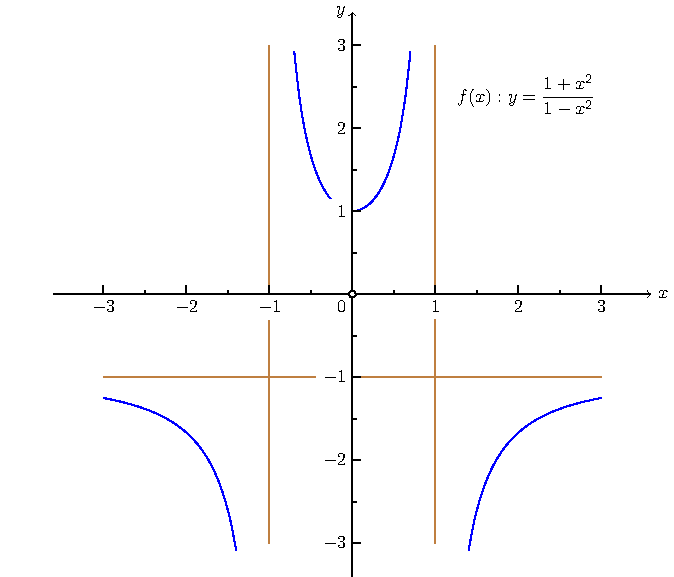
\includegraphics[width=1\linewidth]{MAI007.pdf}
    \captionof{figure}{Graf funkce $f(x):y=\dfrac{1+x^2}{1-x^2}$}
    \label{MAI:fig_007}
  \par}
\end{example}
    %-------------------------------------------------------------------

} %tikzset
%---------------------------------------------------------------------------------------------------
\printbibliography[heading=subbibliography]
\addcontentsline{toc}{section}{Seznam literatury} 
%  %==================================== Primitivní funkce ======================================================
\chapter{Primitivní funkce}
\minitoc
\newpage
  %----------------------------Neurčitý integrál----------------------------------------------------
  \section{Motivace}
    Problém \emph{neurčitého integrálu}, neboli \textbf{primitivní funkce}, lze vyložit velmi jednoduše: 
    Máme podezření, že zadaná funkce \(f(x)\) vznikla derivováním jisté, zatím neznámé, funkce \(F(x)\). 
    Dokážeme ji najít? 
  
    K danému problému můžeme přistupovat také fyzikálně: Zavedením pojmu derivace funkce jsme motivovali 
    důležitým požadavkem definovat okamžitou rychlost pohybu bodu po přímce. Existuje přirozeně i požadavek 
    opačný, tj. nalézt zákon dráhy pohybu bodu po přímce, je-li dána jeho okamžitá rychlost jako funkce 
    času \cite[s.~253]{Brabec1989}. Vše si ukážeme na následujícím příkladu:  
   
    \begin{example}
      Je dána okamžitá rychlost $v$ pohybu bodu po přímce (ose) $x$ rovnicí $v(t) = 2t + 1$, $t\in\langle 
      -\infty,+\infty \rangle$. Najděte zákon dráhy pohybu, je-li známo, že v čase $t = 0$ měl bod polohu 
      $x = x_0$.
      \newline
      \textbf{řešení:}\newline
      Označíme-li $x(t)$ polohu bodu v okamžiku $t$, pak $v(t) = \frac{dx}{dt}$. Hledáme tedy funkci $x = 
      x(t)$, pro níž platí 
      \begin{align}
        \frac{dx}{dt} &= 2t + 1 \qquad x(0) = x_0.  \nonumber \\ 
        \shortintertext{Je ihned patrné, že první podmínce vyhovuje nekonečně mnoho funkcí}
        x(t)          &= t^2 + t + C,           \label{MA:int_ex_09}    \\ 
        \shortintertext{ kde $C$ je libovolná konstanta. Funkce, která splňuje i druhou podmínku 
          (říkáme ji též počáteční podmínka), najdeme z rovnice \ref{MA:int_ex_09} dosazením dané podmínky 
          $t = 0,\ x = x_0$. Dostaneme $x_0 = C$. Dosazením do \ref{MA:int_ex_09} za $C$ plyne hledaný 
          zákon dráhy}
        x(t)          &= t^2+t+x_0.                 \nonumber 
        \shortintertext{Jednoduchou zkouškou se přesvědčíme, že tato funkce splňuje obě dané podmínky a 
          zároveň vidíme, že hledaná primitivní funkce daných vlastností je jediná.}  \nonumber
      \end{align}
    \end{example}\vspace{-1cm}    
    Každé takové funkci, jejíž derivací je daná funkce, budeme říkat \emph{primitivní funkce} k dané 
    funkci. Na uvedeném příkladě je patrné, že k dané funkci může existovat nekonečně mnoho primitivních 
    funkcí. Množinu všech primitivních funkcí se často nazývá \textbf{neurčitým integrálem}. Po tomto 
    názorném uvedení do problému přejděme k přesné formulaci základních pojmů.
    
    \begin{definition} 
      Funkce $F: J\rightarrow \realset$, kde $J\subset \realset$ je interval, se nazývá primitivní funkce k 
      funkci $f$ na intervalu $J$ právě když, pro všechna $x\in J$ je $F'(x) = f(x)$ (v krajních bodech 
      intervalu $J$, pokud k němu patří, jde o derivace jednostranné).
    \end{definition}
    
    \begin{example} 
      K funkci $\sin x$ je primitivní funkcí na libovolném intervalu $J\subset(-\infty,+\infty)$ funkce 
      $-\cos x$, protože $(-\cos x)' = \sin x$. Ale též funkce $3-\cos x$ je primitivní funkcí k funkci $\sin 
      x$, protože $(3 - \cos x)' = \sin x$ pro všechna $x\in(-\infty, \infty)$.
    \end{example}
    
    Je vidět, že rozdíl dvou primitivních funkcí k téže funkci je konstanta. To není náhoda, jak potvrzuje 
    následující věta:
    
    \begin{lemma}
      \begin{enumerate}[label=\itshape\alph*\upshape)]
        \item Je-li funkce $F$ primitivní funkcí k funkci $f$ na intervalu $J$ a $c$ reálná konstanta, pak i 
              funkce $G = F + c$ je primitivní funkcí k funkci $f$ na intervalu $J$.
        \item Jsou-li funkce $F$ a $G$ primitivní funkce k funkci $f$ na intervalu $J$, pak funkce
              $F-G$ je na intervalu $J$ konstantní.
      \end{enumerate} 
      \begin{proof}
        Tvrzení a) plyne z definice protože $G'(x) = [F(x) + c] = F'(x) = f(x)$ pro všechna $x\in
        J$. Tvrzení b) je důsledkem věty \ref{MA1:lem_diff01}.
      \end{proof}
    \end{lemma}
    Neurčitost vyplývá právě z toho, že primitivní funkce není dána jednoznačně, je určena až na konstantu. 
    Značíme
    \begin{equation*}
      \boxed{F(x) = \int f(x)\dx + C}
    \end{equation*}
        
    Jak ale primitivní funkce hledat? V jednoduchých příkladech poslouží tabulka derivací, již čteme „zprava 
    doleva“. (Je dobré si ji uložit do paměti.) Tabulka však pokryje jen velmi málo případů, pouze 
    elementární funkce. Je tedy třeba najít metody, jak při hledání primitivních funkcí postupovat. Nejprve 
    však uvedeme dvě základní pravidla pro primitivní funkce, která plynou z pravidel pro derivování:
    \begin{align}
      \int[f(x)\pm g(x)]\dx &= \int[f(x)\pm g(x)]\dx + \int[f(x)\pm g(x)]\dx \label{MA1:eq_int10} \\
      \int cf(x)\dx         &= c \int f(x)\dx, \qquad \text{\(c\) je konstanta.} \label{MA1:eq_int11}
    \end{align}
  
  \section{Tabulka neurčitých integrálů}\label{MA:chap_tabINT}
    Pokud není nic uvedeno, platí vzorce pro všechna \(x\) a pro všechny hodnoty uvedených
    konstant. Místo platí pro \(x\) z intervalu \((-\infty,0),(0,+\infty)\) píšeme stručně
    \(x\neq0\) apod. Literatura: \cite[p.~396]{Rektorys1963}.
  
    \begin{flalign}
      & \int 0\dx = c                                        &         \label{MA:baseInt01}     \\
      & \int a\dx = ax+c                                     &         \label{MA:baseInt02}     \\
      & \int x^n\dx = \frac{x^{n+1}}{n+1}+c, \qquad
        \begin{cases}
          \forall x\in\realset\,                 
            \text{pro}&\,n\in\naturalset, n>0,         \\
          \forall x\in\realset-\{0\},            
            \text{pro}&\,n\in\naturalset, n<-1,        \\
          \forall x>0,\text{pro}\,n\in\realset\, 
            \text{pro}&\,n\notin\naturalset
        \end{cases}                                          &         \label{MA:baseInt03}     \\
      & \int\frac{1}{x}\dx = 
            \ln\abs{x}+c \hspace{1ex}\forall x\neq0          &         \label{MA:baseInt04}     \\
      & \int e^x \dx       = e^x+c                           &         \label{MA:baseInt05}     \\
      & \int\ln x\dx       = 
          x\ln x - x + c \hspace{1ex}\forall x>0             &         \label{MA:baseInt06}     \\
      & \int a^x \dx     =
          \frac{a^x}{\ln a}+c 
          \hspace{1ex}\forall a>0,\,a\neq1                   &         \label{MA:baseInt07}     \\
      & \int \sin x \dx  = -\cos x                           &         \label{MA:baseInt08}     \\
      & \int \cos x \dx  =  \sin x                           &         \label{MA:baseInt09}     \\
      & \int\frac{1}{\cos^2x}\dx      = 
          \tg x+c   \forall x\neq(2k+1)\pi,\,k\in\naturalset &         \label{MA:baseInt10}     \\ 
      & \int \frac{1}{\sin^2x}\dx     = 
         -\cotg x+c \forall x\neq k\pi,\,k\in\naturalset     &         \label{MA:baseInt11}     \\
      & \int\frac{1}{\sqrt{1-x^2}}\dx =  \arcsin x + c  =  -\arccos x + c 
          \hspace{1ex}\forall x\in(-1,1)\,x\in\realset       &         \label{MA:baseInt12}     \\
      & \int\cosh\dx = \sinh x + c                           &         \label{MA:baseInt13}     \\
      & \int\sinh\dx = \cosh x + c                           &         \label{MA:baseInt14}     \\
      & \int\frac{1}{1+x^2}\dx = \arctg x + c                &         \label{MA:baseInt15}     \\
      & \int \frac{1}{\sqrt{x^2 + 1}}\dx 
        = \ln(x + \sqrt{x^2+1}) + c  
        = \sinh^{-1}x + c                                    &         \label{MA:baseInt16}     \\ 
      & \int \frac{1}{\sqrt{x^2 - 1}}\dx 
        = \ln(x + \sqrt{x^2-1}) + c                   
        = \cosh^{-1}x + c \hspace{1ex}x\in(1,+\infty)        &         \label{MA:baseInt17}     \\
      & \int\frac{1}{\sqrt{x^2+a^2}}\dx 
        = \sinh^{-1} \frac{x}{a} = \ln (x+\sqrt{x^2+a^2})    &         \label{MA:baseInt18}     \\
      & \int \frac{1}{\sqrt{x^2-a^2}}\dx 
        = \cosh^{-1} \frac{x}{a} = \ln (x+\sqrt{x^2-a^2})    &         \label{MA:baseInt19}     
    \end{flalign}
    \vspace{-2.9em}
    \begin{flalign}
      & \int\frac{1}{\sqrt{x^2-1}}\dx 
        = \left\{ 
          \begin{array}{l l}
            \ln\abs{x+\sqrt{x^2-1}}+c      & \quad \text{pro \(\abs{x}>1\)}  \\
            \cosh^{-1}x+c                  & \quad \text{pro \(\abs{x}<1\)}
          \end{array} 
          \right.                                            &         \label{MA:baseInt20}     
    \end{flalign}
    \vspace{-2.9em}
    \begin{flalign}
      & \int\tan x \dx = \ln |\sec x| + c                    &         \label{MA:baseInt21}     
    \end{flalign}
    \vspace{-2.9em}
    \begin{flalign} 
      & \int\sec x \dx = \ln |\sec x + \tan x| + c           &         \label{MA:baseInt22}     
    \end{flalign}
    \vspace{-2.9em}
    \begin{flalign}
      & \int\sec^2 x \dx     = \tan x + c                    &         \label{MA:baseInt23}     
    \end{flalign}
    \vspace{-2.9em}
    \begin{flalign}
      & \int\sec x\tan x \dx = \sec x + c                    &         \label{MA:baseInt24}     \\
      & \int\frac{a}{a^2+x^2}\dx = \tan^{-1}\frac{x}{a}      &         \label{MA:baseInt25}     \\
      & \int\frac{a}{a^2-x^2}\dx = 
          \frac{1}{2}\ln\left|\frac{x+a}{x-a}\right|         &         \label{MA:baseInt26}     \\
      & \int\frac{1}{\sqrt{a^2-x^2}} \dx = 
          \sin^{-1} \frac{x}{a}                              &         \label{MA:baseInt27}     \\
      & \int\frac{a}{x\sqrt{x^2-a^2}}\dx = 
          \sec^{-1} \frac{x}{a}                              &         \label{MA:baseInt28}    
    \end{flalign}     
    
  \section{Metody určení primitivní funkce}
    Procesu hledání primitivní funkce se často říká integrování nebo integrace (od slova “integrál”), což z 
    matematického hlediska znamená provést inverzní operaci k operaci derivování. Smutnou zprávou je, že na 
    rozdíl od derivování neexistuje obecný vzorec pro integrování součinu či podílu, ani obecný vzorec pro 
    integrování složených funkcí. Při hledání integrálů složitějších funkcí se využívá např. 
    \emph{linearita, metoda per partes, substituční metoda}, popř. některé další speciální metody. Řešitel 
    v mnoha případech musí projevit důvtip a intuici, která mu pomůže nalézt primitivní funkci k dané 
    funkci.
  
    % --------------------------Integrace po částech - per partes-------------------------------------------
    \subsection{Integrace po částech - per partes}
      Metoda integrace \emph{per partes} neboli \emph{po částech} využívá vzorce pro derivaci součinu 
      funkcí. Připomeňme si jej: Pro derivaci součinu dvou funkcí \(u(x)\) a \(u(x)\) platí
      \cite[p.~137]{Musilova2009MA1}.
      \begin{align}
        [u(x)v(x)]' &= u(x)'v(x) + u(x)v'(x).  \label{MA:eq_Int29} \\
        \shortintertext{Primitivní funkcí levé strany je \(F(x) = u(x)v(x)\), a tedy}
        u(x)v(x)    &=  \int u'(x)v(x)\dx + \int u(x)v'(x)\dx \nonumber
      \end{align}  
      za předpokladu, že existují obě primitivní funkce na pravé straně. K čemu může tento samozřejmý 
      vzorec sloužit při hledání primitivní funkce? Dejme tomu, že zadaná funkce \(f(x)\), k níž máme 
      hledat funkci primitivní, je tvaru \(f(x) = u'(x)v(x)\), a my si s ní nevíme rady. Je však možné, že 
      bychom si docela dobře poradili s primitivní funkcí k funkci \(g(x) = u(x)v(x)\). A předchozí vzorec 
      umožňuje nahradit výpočet neurčitého integrálu z funkce \(f(x)\) výpočtem neurčitého integrálu z 
      funkce \(g(x)\), tedy
      \begin{equation}\label{ma:eq_perpartes}
        \int u'(x)v(x)\dx = u(x)v(x) - \int u(x)v'(x)\dx 
      \end{equation}
      \begin{example}
        Máme za úkol najít primitivní funkci k funkci \(f(x) = x\sin x\). Představíme-li si ji jako součin 
        \(f(x) = u'(x)v(x)\), kde \(u'(x) = \sin x\), tj. \(u(x) = —\cos x\), a \(v(x)= x\), tj. \(v'(x) 
        = 1\), dostaneme
        \begin{equation*}
          \int x\sin x\dx = -x\cos x + \int\cos x\dx = -x\cos x + \sin x + C.
        \end{equation*}          
      \end{example}
      Není vždy jednoduché rozpoznat, jak máme rozložit funkci \(f(x)\) na součin funkcí \(u'(x)\) a 
      \(v(x)\). Takový rozklad není určen jednoznačně a požadavek na něj bychom mohli (dosti nepřesně) 
      formulovat tak, aby funkce \(v'(x)\) byla jednodušší než v \(v(x)\) (například derivováním polynomu 
      se snižuje jeho stupeň) a funkce \(u'(x)\) a \(u(x)\) aby byly zhruba „stejně složité“ (například 
      \(u'(x) =e^x\), \(u(x) = e^x\), nebo \(u'(x) = \cos x\), \(u(x) = \sin x\), apod.). Spolehlivě 
      používat metodu per partes se však můžeme naučit pouze studiem vyřešených příkladů z literatury a 
      praktickým procvičováním \cite[p.~138]{Musilova2009MA1}.
      
      \begin{example}
        (\emph{Umělý rozklad na součin}): Někdy zadaná funkce \(f(x)\) jako součin vůbec nevypadá, a přesto 
        je použití metody per partes vhodné. Například pro elementární funkci \(f(x) = \ln x\) sice najdeme 
        primitivní funkci \ref{MA:baseInt06} v tabulce základních neurčitých integrálů z odstavce 
        \ref{MA:chap_tabINT}, ale je možné postupovat i jinak. Představme si \(f(x)\) jako součin 
        \(f(x) = 1\cdot\ln x\) a zvolme \[u'(x) = 1 ⇒ u(x) = x, \qquad v(x) = lnx ⇒ v'(x) = \frac{1}{x}\] 
        Pak \[\int \ln\dx = x\ln x - \int x\cdot\frac{1}{x}\dx = x\ln x - x.\]
      \end{example}
  
    %--------------------------- Substituční metoda ----------------------------------------------
    \subsection{Substituční metoda I}
      Tato metoda \emph{substituce} neboli \emph{náhrady} spočívá v tom, že vhodně zvolenou funkci 
      obsaženou v předpisu \(f(x)\) označíme jako novou jednoduchou proměnnou. Čeho tím dosáhneme? 
      Předpokládejme například, že \[f(x)=\varphi'(x)g[\varphi(x)]\] a označme jako novou proměnnou \(u = 
      f(x)\). Že to vypadá, jako bychom se chystali použít vzorec pro derivaci složené funkce? Správně! 
      Dejme tomu, že známe primitivní funkci \(G(u)\) k funkci \(g(u)\). Pak platí
      \begin{align*}
       \left[G\left(\varphi(x)\right)\right]' 
          &= G'\left[\varphi(x)\right]\cdot\varphi'(x) =
             g\left[\varphi(x)\right]\cdot\varphi'(x), \qquad\text{a tedy}   \\
       \int \varphi'(x) g\left[\varphi(x)\right]\dx &=  G\left[\varphi(x)\right]. 
      \end{align*}      
      Na základě těchto úvah formulujeme následující větu:
      \begin{lemma}
        Jestliže
        \begin{equation}\label{ma:eq_subst1}
          \int{f(u)du}=F(u)+C
        \end{equation}
        a $u=\varphi(x)$, pak
        \begin{equation}\label{ma:eq_subst2}
            \int{f[\varphi(x)]\varphi'(x)du}=F(\varphi(x))+C
        \end{equation}
      \end{lemma}
  
      Základem úspěchu při aplikací věty je správný výběr funkce $\varphi(x)$. Praxe je totiž
      taková, že výpočet konkrétních příkladů je schématicky veden od rov. \ref{ma:eq_subst2} ke
      vzorci rov. \ref{ma:eq_subst1}.
      
      \begin{example} Jak poznat kandidáta na substituční metodu I
        Počítejme neurčitý integrál \[\int \frac{x}{\sqrt{x^2+1}}.\]
        Vidíme, že čitatel funkce za integrálem je až na násobení konstantou derivací výrazu pod odmocninou. 
        Při označení \(u=\varphi(x) = x^2 + 1\) dostáváme \(\varphi'(x) = x\), 
        \begin{equation*}
          \int\frac{x}{\sqrt{x^2+1}}\dx = \frac{1}{2}\int\frac{2x}{\sqrt{x^2+1}}\dx
                                        = \frac{1}{2}\int\frac{1}{\sqrt{u}}\dd{u} = \sqrt{u} + C 
                                        = \sqrt{x^2 + 1} + C  
        \end{equation*}
      \end{example}
      
      \begin{example}\label{ma:ex_sub_metoda}$\displaystyle\int{e^{x^{x^2}}dx}$
        \begin{equation*}
            \int{e^{x^{x^2}}dx}=
               \left[
                 \begin{array}{c}u=x^2 \\ du=2xdx\end{array}
               \right]=
               \frac{1}{2}\int{e^udu}=\frac{1}{2}e^u=\frac{1}{2}e^{x^2}+C.
        \end{equation*}
      \end{example}
      \begin{example}$\displaystyle\int{x^3e^{x^4}}dx \qquad x\in R$
        \begin{align*}
          \displaystyle\int{x^3e^{x^4}}dx
             &= 
             \left[
               \begin{array}{cc}
                  u=x^4   & du=4x^3dx \Rightarrow \displaystyle\frac{du}{4} = x^3dx  \\
               \end{array}
             \right]                                                                           \\
             &= \frac{1}{4}\int{e^u}du = \frac{e^u}{4} = \frac{e^{x^4}}{4} + C 
        \end{align*}
      \end{example}

    % -------------------Substituční metoda II----------------------------------------------------------------
    \subsection{Substituční metoda II}
      Druhý typ substituční metody spočívá naopak v tom, že na místo původní proměnné \(x\) dosadíme vhodnou 
      funkci \(x = \psi(t)\). Místo primitivní funkce k funkci \(f(x)\) pak hledáme primitivní funkci k 
      funkci \(g(t) = f[\psi(t)]\psi'(t)\). Skutečně, je-li \(F(x)\) primitivní funkcí k \(f(x)\), pak 
      derivací složené funkce \(G(t) = F[\psi(t)]\) dostaneme
      \begin{equation*}
       G'(t) = F'[\psi(t)]\psi'(t) = f[\psi(t)]\psi'(t) = g(t).
      \end{equation*}
      \begin{example} Náhrada proměnně \(x\) funkcí
        Typické jsou neurčité integrály, které vedou na goniometrické substituce, například
        \[\int\sqrt{1-x^2}\dx\]
        
        Označme \(x=\psi(t)=\sin(t)  \Rightarrow \psi'(t)=\cos(t)\) a můžeme psát
        \begin{align*}
          \int\sqrt{1-x^2}\dx 
            &= \int\sqrt{1-\sin^2t}\cos t\dd{t} = \int\cos^2 t \dd{t} = \int\frac{1+\cos2t}{2}\dd{t}\\
          \frac{1}{2}t+\frac{\sin2t}{4}+C
            &= \frac{1}{2}\arcsin x + \frac{2\sin t\cos t}{4} 
             = \frac{1}{2}\arcsin x + \frac{x\sqrt{1-x^2}}{2} + C.
        \end{align*}
        Správně bychom měli místo \(\sqrt{1 - \sin^2x}\) psát \(\abs{\cos x}\). Vzhledem k tomu, že jde o 
        neurčitý integrál, je možné hledat primitivní funkci na intervalu, kde platí \(\cos x = \abs{\cos 
        x}\).
      \end{example}
      Jistě nám neuniklo, že princip substitučních metod I a II je stejný. Jsou totiž obě založeny na použití 
      pravidla pro derivaci složené funkce.
  
    % ---------Integrování součtu, úprava integrandu a integrování rozkladem----------------------------------
    \subsection{Integrování součtu, úprava integrandu a integrování rozkladem}
      \begin{example}
        Zdroj \cite[s.~29]{Knichal}.
        \begin{equation}\label{MA:int_ex_01}
          \int{\frac{x^4+3x^3-3x^2+3x}{x^2+1}\dx}
        \end{equation}
        Dělením čitatele integrandu jmenovatelem  dostaneme rozklad integrandu na součet funkcí,
        jejich integrály najdeme snadno:
         \begin{equation*} 
           \polylongdiv[style=C,div=:]{x^4+3x^3-3x^2+3x}{x^2+1}
         \end{equation*}
         \begin{align*}
           \shortintertext{Tedy}
           \frac{x^4+3x^3-3x^2+3x}{x^2+1}                 &= x^2+3x-4+\frac{4}{x^2+1} \\
           \intertext{Pro uvedený integrál dostaneme} 
           \int{\frac{x^4+3x^3-3x^2+3x}{x^2+1}\dx}        &=                 \\
           \int{\left(x^2+3x-4+\frac{4}{x^2+1}\right)\dx} &= 
             \frac{x^3}{3}+\frac{3x^2}{2}-4x+4\arctan x + C.
         \end{align*}
      \end{example}
      
      \begin{example}
        Zdroj \cite[s.~29]{Knichal}.
        \begin{equation}\label{MA:int_ex_03}
          \int\frac{3}{(1+x^2)x^2}\dx
        \end{equation}
        Integrand upravíme přičtením a odečtením výrazu $3x^2$ v čitateli zlomku takto:
        \begin{align*}
          \frac{3}{(1+x^2)x^2} 
            &= \frac{3+3x^2-3x^2}{(1+x^2)x^2} = \frac{3}{x^2}-\frac{3}{1+x^2}                      \\  
          \intertext{Tedy v každém otevřeném intervalu, který neobsahuje bod \(x=0\), platí}
          \int{\frac{3}{(1+x^2)x^2}\dx} 
            &= 3\int{\frac{1}{x^2}dx} - 3\int{\frac{1}{1+x^2}dx}                                   \\
            &= -\frac{3}{x}-3\arctan x + C. 
        \end{align*}
      \end{example}
      
      \begin{example}
        Zdroj \cite[s.~30]{Knichal}.
        \begin{equation}\label{MA:int_ex_04}
          \int{\sqrt{1+\cos2x}\dx}
        \end{equation}
        Funkci $\sqrt{1+\cos2x}$ upravíme na základě goniometrické identity \ref{MA1:eq_cos2x}
        \begin{align*}
          1+\cos2x       &= 1+\cos^2x-\sin^2x=2\cos^2x                                         \\
          \shortintertext{takto}
          \sqrt{1+\cos2x}&=\sqrt{2\cos^2x} = \sqrt{2}|\cos x| = \varepsilon\sqrt{2}\cos x,     \\
          \shortintertext{kde}
          \varepsilon &=
            \begin{cases} 
             +1, &  x\in \left(-\frac{\pi}{2}+2n\pi,\frac{\pi}{2}+2n\pi\right), \\
             -1, &  x\in \left(\frac{\pi}{2}+2n\pi,\frac{3\pi}{2}+2n\pi\right),
            \end{cases}                                                                        \\
          \intertext{$n$ je přirozené číslo. Proto pro $x$ ležící v uvedených intervalech je}
          \int\sqrt{1+\cos2x}\dx & = \varepsilon\sqrt{2}\int\cos x\dx 
                                   = \varepsilon\sqrt{2}\sin x + C.
        \end{align*}
      \end{example}
      
      \begin{example}
        Zdroj \cite[s.~30]{Knichal}.
        \begin{equation}\label{MA:int_ex_05}
          \int\cos^2\frac{x}{2}\dx
        \end{equation}
        Integrand upravíme na součet dvou tabulkových integrálů použitím vzorce
        \begin{align*}
          \cos^2\frac{x}{2} &= \frac{1}{2}(1+\cos x)     \\ 
          \shortintertext{takže}
          \int{\cos^2\frac{x}{2}}\dx 
                            &= \frac{1}{2}\int{(1+\cos x)}\dx = \frac{1}{2}(x+\sin x) + C.
        \end{align*}          
      \end{example}
      
      \begin{example}
        Zdroj \cite[s.~30]{Knichal}.
        \begin{equation}\label{MA:int_ex_06}
          \int{\tan^2x}\dx
        \end{equation}
        funkci napíšeme ve tvaru 
        \begin{align*}
          \tan^2x &= \frac{\sin^2x}{\cos^2x}=\frac{1-\cos^2x}{\cos^2x} = \frac{1}{\cos^2x}-1   \\
          \shortintertext{takže}
          \int{\tan^2x}dx &= \int{\left(\frac{1}{\cos^2x}-1\right)}\dx = \tan x - x + C.  
          \intertext{$\forall x\in\left(-\frac{\pi}{2}+k\pi, \frac{\pi}{2}+k\pi\right)$,
                     $k\in\naturalset$.}
        \end{align*}          
        
      \end{example}
      
      \begin{example}
        \begin{equation}\label{MA:int_ex_07} 
          \int\frac{\cos2x}{\cos^2x\cdot\sin^2x}\dx, 
            \qquad (\sin^2x\cos^2x\neq0; x\neq k\frac{\pi}{2}; k\in Z)
        \end{equation} 
       Integrand upravíme pomocí vzorce pro dvojnásobný úhel \ref{MA1:eq_cosx2}:
        \begin{equation*}
          \int\frac{\cos^2x-\sin^2x}{\cos^2x\cdot\sin^2x}\dx = 
            \int\frac{1}{\sin^2x}\dx - \int\frac{1}{\cos^2x}\dx = -\cot x - \tan x + C.
        \end{equation*}
      \end{example}
      
      \begin{example}
       \begin{equation}\label{MA:int_ex_08}
         \int\frac{1}{\cos x\cdot\sin x}\dx, 
           \qquad (\sin x\cos x\neq0; x\neq k\frac{\pi}{2}; k\in Z)
       \end{equation}
       Integrand rozšíříme o funkci $\displaystyle{\frac{1}{\cos^2x}}$
        \begin{equation*}
          \bigintss\dfrac{\dfrac{1}{\cos^2x}}{\dfrac{\sin x\cdot\cos x}{\cos^2x}} \dx = 
          \bigintss\dfrac{\dfrac{1}{\cos^2x}}{\tan x}\dx = \ln\abs{\tan x} + C.
        \end{equation*}            
      \end{example}
  
    %--------------------------- Integrace racionální funkce--------------------------------------
    \subsection{Integrace racionální funkce}
      Některé příklady v předchozím odstavci, (viz např. \ref{MA:int_ex_01} a 
      \ref{MA:int_ex_02}) jsme dělením čitatele integrandu jmenovatelem dostali rozklad
      integrandu na součet racionální funkce (polynomu) a ryze lomené racionální funkce.
      Integrování polynomu je snadné, neboť jde o součet integrálů tvaru $\int c_kx^k dx$, kde
      $k$ je celé nezáporné číslo. Omezíme se tedy na integrování \emph{ryze lomené racionální
      funkce},  tj. funkce ve tvaru $P(x)/Q(x)$, kde $P(x), Q(x)$ jsou polynomy, přičemž stupeň
      polynomu $P(x)$ je menší než stupeň polynomu $Q(x)$. Taková funkce může vzniknout součtem
      několika jednoduchých zlomků.
      
      \begin{example}
        Upravte
        \begin{align*}
          \frac{1}{x-1}+\frac{x+2}{x^2+x+3} 
            & = \frac{x^2+x+3+x^2+x-2}{(x-1)(x^2+x+3)}              \\
            & = \frac{2x^2+2x+1}{x^3+2x-3}
        \end{align*}          
      \end{example}
      
      Jsme tedy vedeni myšlenkou, zda naopak každá ryze lomená racionální funkce se dá rozložit
      na součet jednoduchých zlomků určitého tvaru - budeme jim říkat \texttt{parciální zlomky},
      které umíme integrovat. Tím se budume zabývat v dalších odstavcích. 
            
      \begin{example}
        \begin{equation}
          \int\frac{1}{x^2 - x + 1}\dx, \qquad x\in R
        \end{equation}
        Kvadratický polynom ve jmenovateli upravíme na čtverec $f(x) = (x + m)^2 + n$:
        \begin{align*}
          \int\dfrac{1}{\left(x-\dfrac{1}{2}\right)^2+\dfrac{3}{4}}\dx   &=
            \dfrac{1}{\sqrt{1-\left(\dfrac{1}{2}\right)^2}}\arctan
            \dfrac{x-\dfrac{1}{2}}{\sqrt{1-\left(\dfrac{1}{2}\right)^2}}                       \\
          \dfrac{2}{\sqrt{3}}\arctan\dfrac{2x-1}{\sqrt{3}}               &=
            \dfrac{2\sqrt{3}}{3}\arctan\dfrac{\sqrt{3}(2x-1)}{3} + C
        \end{align*}
      \end{example}     
      
      \begin{definition} Parciální (částečným) zlomkem, budeme nazývat zlomek tvaru
         \begin{equation}
            \frac{A}{(x-\alpha)^k} \qquad\text{nebo}\qquad\frac{Mx + N}{x^2 + px +q}
         \end{equation}  
         $A,\ M,\ N,\ \alpha\ , p,\ q$ reálné $p^2-4q < 0$, $k$ celé nezáporné.         
      \end{definition}
      
      Integrál prvního zlomku, tj. $\displaystyle{\int\frac{A}{(x-\alpha)^k}\dx}$, vypočteme substitucí 
      $x-\alpha=t$, odtud plyne $dx = dt$,
      \begin{equation}\label{MA:int_ex_14}
        \int\frac{A}{(x-\alpha)^k}dx = \int\frac{A}{t^k}dt.
      \end{equation}
      Tento integrál se rovná
      \begin{equation}\label{MA:int_ex_16}
        -\frac{A}{k-1}\frac{1}{(x-\alpha)^{k-1}} + C.
      \end{equation}        
      je-li $k>1$, a rovná se $A\ln|x-\alpha| + C$, je-li $k = 1$. Výsledek platí na každém
      intervalu neobsahujícím bod $\alpha$.
      
       U integrál druhého zlomku uvedeme postup výpočtu pro $k = 1$. 
      \begin{align*}
         \intertext{\(\displaystyle\int{\frac{Mx + N}{x^2+px+q}dx}\)}
           \qquad &=  \int{\frac{Mx}{x^2+px+q}dx} + \int{\frac{N}{x^2+px+q}dx}                     \\  
           \qquad &=  \frac{M}{2}\int{\frac{(2x + p) - p}{x^2+px+q}dx} + 
                     N\int{\frac{1}{x^2+px+q}dx}                                                   \\ 
           \qquad &=  \frac{M}{2}\int{\frac{2x + p}{x^2+px+q}dx} + 
                      \left(N-\frac{Mp}{2}\right)\int{\frac{1}{x^2+px+q}dx.}                   
      \end{align*}  
      
      Z naznačeného postupu je vidět hlavní myšlenka: upravit integrál na lineární kombinaci dvou integrálů, 
      z nichž první má v čitateli integrandu derivaci jmenovatele a je podle příkladu *** roven 
      $\ln|x^2+px+q|$ kde $x^2+px+q >0$ pro $x\in R$ a integrand druhého integrálu má čitatel konstantní.
      
      Výpočet druhého integrálu probíhá takto: 
      \begin{equation}\label{MA:int_ex_10}
        \int\dfrac{1}{x^2+px+q}\dx = 
          \int\dfrac{1}{\left(x+\dfrac{p}{2}\right)^2 + q - \dfrac{p^2}{4}}\dx;
      \end{equation}
      substitucí $x+\dfrac{p}{2} = t\sqrt{q - \dfrac{p^2}{4}}$ dostáváme dále
      \begin{equation*}\label{MA:int_ex_11}
        \bigints{\frac{1}{\displaystyle{\left(x+\frac{p}{2}\right)^2 + q - \frac{p^2}{4}}}}dx 
          =\displaystyle{
            \bigints{
              \frac{\sqrt{q-\frac{p^2}{4}}}{\left(q-\frac{p^2}{4}\right)(t^2+1)}}dt
            }   
      \end{equation*}
      po úpravě dostaneme tabulkový integrál
      \begin{equation}\label{MA:int_ex_12}
        \frac{1}{\sqrt{q-\frac{p^2}{4}}}\int{\frac{dt}{t^2+1}},
      \end{equation}
      jehož řešení je  
      \begin{equation*}\label{MA:int_ex_13}
        \frac{1}{\sqrt{q-\frac{p^2}{4}}}\arctan{t} 
          = \sqrt{q-\frac{p^2}{4}}\arctan\frac{x+\frac{p}{2}}{\sqrt{q-\frac{p^2}{4}}}.     
      \end{equation*}   
      Z postupu je opět vidět hlavní myšlenka: úprava integrandu na tvar $\dfrac{1}{t^2+1}$.
      Jmenovatel $x^2+px+q$ jsme doplnili na úplný čtverec a užili uvedenou substituci (uvažme,
      že $q-\dfrac{p^2}{4}>0$, protože diskriminant $\dfrac{p^2}{4}-q$ trojčlenu $x^2+px+q$ je
      podle předpokladu záporný). Výsledek platí u obou integrálu v intervalu \((-\infty,
      +\infty)\).
      
      % -----------------------Funkce typu {f(x)=\sqrt{ax+b}} ------------------------------------
      \subsubsection*{Funkce typu $\boxed{f(x)=\sqrt{ax+b}}$ :}
         Funkci, jež je dána rovnicí, jež obsahuje polynomy proměnné x  ve výrazu $\sqrt{ax+b}$,
         v němž $ax+b>0$, $a>0$, integrujeme pomocí substituce:
         \begin{equation}\label{ma:eq_sub_fce1}
             u=\sqrt{ax+b},\quad du=\frac{1}{2}\frac{a}{u}dx,\quad dx=2\frac{u}{a}du
         \end{equation}
         Je-li potřeba dosadit do integrované funkce také za $x$, vyjádříme ze substituční
         rovnice $x=\frac{u^2-b}{a}$.
      % ----------------------Funkce typuf(x)=\frac{1}{\sqrt{x^2+a}}, a\neq0 -------------------- 
      \subsubsection*{Funkce typu $\boxed{f(x)=\frac{1}{\sqrt{x^2+a}}}, a\neq0$ :}
         \begin{example}\label{ma:ex_sub_metoda1}$\displaystyle\int{\frac{1}{\sqrt{x^2+a}}dx}$:\vskip0.5mm
           \textbf{Řešení}: Užijeme \textbf{Eulerovu substituci}\vskip1mm 
                            \hskip17mm$u=x+\sqrt{x^2+a},\quad \displaystyle{du=\frac{u}{\sqrt{x^2+a}}dx}$,
                            $\displaystyle{\frac{du}{u}=\frac{dx}{\sqrt{x^2+a}}}.$
           \begin{equation*}
            \int{\frac{1}{\sqrt{x^2+a}}dx}=\int{\frac{du}{u}}=\ln|u|=\ln|x+\sqrt{x^2+a}|+C
           \end{equation*}
         \end{example}
  
    % --------------------------Integrály goniometrických funkcí----------------------------------     
    \subsubsection{Integrace goniometrických funkcí}
      
    % ---------------- Rozklad ryze lomené funkce v parciální zlomky -----------------------------------------
    \subsubsection{Rozklad ryze lomené funkce v parciální zlomky}
      Nechť je dána racionální funkce $R = \frac{P}{Q}$ s reálnými koeficienty. Můžeme
      předpokládat, že je \emph{ryze lomenná}\footnote{tj. stupeň polynomu $P$ je menší než
      stupeň polynomu $Q$}. Pokud by tomu tak nebylo, dostaneme dělením čitetele jmenovatelem
      zlomku součet polynomu a ryze lomené racionální funkce.
      
      \begin{example}$\displaystyle\int{\frac{8x-31}{x^2-9x+14}}dx$\cite[s.~90]{Knichal}\newline
        Kořeny polynomu ve jmenovateli $\alpha_1 = 2$, $\alpha_2 = 7$ jsou jednoduché - každému z
        nich bude v rozkladu odpovídat jen jeden člen $$\frac{8x-31}{x^2-9x+14} = \frac{A}{x-2}
        + \frac{B}{x-7}.$$ Členy mnohočlenu na pravé straně seřadíme podle mocnin $x$ $$8x-31 =
         x(A+B)+(7A-2B).$$ Porovnáním odpovídajících si koeficientů dostaneme
        \begin{align*}
          8   &=   \; A + \, B \\
          -31 &= -7A - 2B
        \end{align*}
        Řešením této soustavy je $A = 3, B = 5$. Platí tedy (pro všechna $x \neq 2$ a $x \neq 7$)
        $$\frac{8x-31}{x^2-9x+14} = \frac{3}{x-2} + \frac{5}{x-7}.$$
        \begin{align*}
          \int{\frac{8x-31}{x^2-9x+14}}dx 
            &= \int{\frac{3}{x-2}}dx + \int{\frac{5}{x-7}}dx      \\
            &= 3\ln|x-2| + 3\ln|x-7| + C.
        \end{align*}
        Výsledek platí v každém intervalu, který neobsahuje body $x = 2$,$x = 7$.
      \end{example}
      
      \begin{example}\label{MA:eq_ex1}$\displaystyle\int{\frac{19x+15}{x^2-x-2}}dx \qquad x\in
        R-\{1,2\} $ \newline Kořeny polynomu ve jmenovateli $\alpha_1 = -1$, $\alpha_2 = 2$ jsou
        jednoduché - každému z nich bude v rozkladu odpovídat jen jeden člen: 
        \begin{align*}
          \frac{19x+15}{x^2-x-2}     &= \frac{A}{x+1} + \frac{B}{x-2} \\
                           19x +15   &= A(x-2) + B(x+1)               \\
                           19x +15   &= x(A+B) - 2A + B               \\
                           19        &= A + B                         \\
                                15   &=        - 2A + B
        \end{align*}              
        Řešením této soustavy je $A = \frac{4}{3}$, $B = \frac{53}{3}$.
        \begin{equation*}
          = \frac{4}{3}\int{\frac{1}{x+1}}dx+\frac{53}{3}\int{\frac{1}{x-2}}dx 
          = \frac{4}{3}\ln|x+1| - \frac{53}{3}\ln|x-2| +  C
        \end{equation*}      
      \end{example}
  
      \begin{example}
        $\displaystyle\int{\frac{2x^2+34x+14}{x^3-4x^2-x-4}}dx$\cite[s.~90]{Knichal}\newline
        Polynom $Q(x)=x^3-4x^2-x-4$ má kořeny $\alpha_{1,2}=\pm1$, $\alpha_{3}=-4$, které jsou
        jednoduché tj. $Q(x)=(x-1)(x+1)(x+4)$ $$\frac{2x^2+34x+14}{x^3-4x^2-x-4} =
        \frac{A}{x-1}+\frac{B}{x+1}+\frac{C}{x+4}$$ Vynásobíme-li tuto rovnici společným
        jmenovatelem zlomků pravé strany (polynomem $Q(x)$), dostaneme
        \begin{align*}
          2x^2+34x+14 &= A(x+1)(x+4)+B(x-1)(x+4)+C(x-1)(x+1) \\
          \intertext{čili}
          2x^2+34x+14 &= A(x^2+5x+4)+B(x^2+3x-4)+C(x^2-1) \\
          2x^2+34x+14 &= (A+B+C)x^2+(5A+3B)x + (4A-4B-C)
        \end{align*}
        Porovnáním odpovídajících si koeficientů u stejných mocnin $x$  dostaneme pro nez\-ná\-mé
        koeficienty $A, B, C$ soustavu rovnic
        \begin{align*}
        % \nonumber to remove numbering (before each equation)
           A+   B + C &= 2 \\
          5A + 3B     &= 34 \\
          4A - 4B - C &= 14
        \end{align*}
        Řešením této soustavy je $A = 5, B = 3, C = -6$ a tedy
        $$\frac{2x^2+34x+14}{x^3-4x^2-x-4} = \frac{5}{x-1}+\frac{3}{x+1}-\frac{6}{x+4}$$
        \begin{align*}
          \int{\frac{2x^2+34x+14}{x^3-4x^2-x-4}}dx 
            &= \int{\frac{5}{x-1}}dx + \int{\frac{3}{x+1}}dx + \int{\frac{6}{x+4}}dx            \\
            &= 5\ln|x-1| +  3\ln|x+1| - 6\ln|x+4| +C.
        \end{align*}
      \end{example}
  
      \begin{example}$\displaystyle{\int\frac{2x+3}{2x^3+2}dx} \qquad x\in R-{-1}$\newline
        a
      \end{example}

  % ---------------- Sbírka řešených příkladů ----------------------------------------------------------------
  \newpage
  \section{Sbírka řešených příkladů}
    Hledej primitivní funkce \(F(x)\) k následujícím funkcím
    
  \begin{example}\(\displaystyle\int{xe^x\dx}\)
    \begin{equation*}
        \int{xe^xdx}=
          \left[\begin{array}{cc}
            u=x   & dv=e^x \\
            du=dx & v=e^x
          \end{array}\right]=
          xe^x-\int{e^x\dx} = xe^x - e^x+C
    \end{equation*}
  \end{example}
  
  \begin{example}$\displaystyle\int{\arctan xdx} \qquad x\in R$
    \begin{align*}
       \int{\arctan xdx}                      &= 
         \left[\begin{array}{cc} 
                  u =\arctan x                     &  dv= 1  \\ 
                 du =\displaystyle\frac{1}{x^2+1}  &   v= x
               \end{array}
         \right]  =                                                                  \\
       x\arctan x-\int\frac{x}{x^2+1}         &= 
         \left[\begin{array}{c} 
                  x^2 + 1 = t  \Rightarrow 2xdx = dt        \\ 
                      xdx = \displaystyle{\frac{dt}{2}}
               \end{array} 
         \right] =                                                                   \\ 
       x\arctan x-\frac{1}{2}\int\frac{dt}{t} &= x\arctan x-\frac{1}{2}\ln|t|        \\
         &=   x\arctan x-\frac{1}{2}\ln|1+x^2|+C                                     \\
    \end{align*}
  \end{example}
  
  \begin{example}$\displaystyle\int{\sqrt{x^2+a}dx}$, kde $a\neq0, x^2+a>0$
    \begin{align*}
      \int{\sqrt{x^2+a}\dx}                           &=
        \left[
          \begin{array}{cc} 
             u =\sqrt{x^2+a}              & dv = 1 \\ 
            du =\displaystyle
                  \frac{x}{\sqrt{x^2+a}}  &  v = x
          \end{array}
        \right]                                                                                   \\
      x\sqrt{x^2+a}-\int{\frac{x^2}{\sqrt{x^2+a}}\dx} &= 
        \displaystyle{x\sqrt{x^2+a}-\int{\frac{x^2+a-a}{\sqrt{x^2+a}}\dx}}                        \\
      \int{\sqrt{x^2+a}\dx}                           &= 
        \displaystyle{x\sqrt{x^2+a}-\int{\sqrt{x^2+a}\dx} + \int{\frac{a}{\sqrt{x^2+a}}\dx}}      \\
      \int{\sqrt{x^2+a}\dx}                           &= 
        \frac{1}{2}\left[x\sqrt{x^2+a}+a\int{\frac{1}{\sqrt{x^2+a}}}\dx\right]
    \end{align*}
    Integrál na pravé straně vyjádříme podle příkladu \ref{ma:ex_sub_metoda1}
    $\displaystyle{\int{\frac{1}{\sqrt{x^2+a}}\dx}}$ a výsledek do\-sta\-ne\-me ve tvaru
    $$\int\displaystyle{{\sqrt{x^2+a}\dx}=\frac{1}{2}\left[x\sqrt{x^2+a}+a\ln{|x +
    \sqrt{x^2+a}|}\right]}$$
  \end{example}
  
  \begin{example}
    \begin{equation}\label{MA:int_ex_02}
      \int{\frac{2x^4-5x^2+14x+13}{x^2-x-2}\dx} \qquad x\in R - \{1,2\}
    \end{equation}
    Dělením čitatele integrandu jmenovatelem dostaneme rozklad integrandu na součet funkcí, jejich integrály 
    najdeme snadno:
    \begin{widetext}
      \begin{equation*}
        \polylongdiv[style=C,div=:]{2x^4-5x^2+14x+13}{x^2-x-2}
      \end{equation*}
    \end{widetext}
    Zbytek po dělení představuje integrál, jež je počítán v příkladu \ref{MA:eq_ex1} a proto ho vynecháme.
    \begin{align*}
       &= 2\int x^2\dx + 2\int x\dx + \int\dx + \int\frac{19x+15}{x^2-x-2}\dx     \\
       &= \frac{2}{3}x^3 + x^2 + x + \frac{4}{3}\ln|x+1| - \frac{53}{3}\ln|x-2| + C 
    \end{align*}                
  \end{example}
    
  \printbibliography[heading=subbibliography]
  \addcontentsline{toc}{section}{Seznam literatury}
%  %====================================================================================================
% --------------------------------------------- Definite Integral -----------------------------------
\chapter{Určitý integrál}
\minitoc
\newpage  
\section{Motivace} 
  %----------------------------------
  % image: MAI_animated_integral.tex label: \label{MAI:fig_anim_int}
    % \documentclass{book}
% \usepackage{ifthen}
% \usepackage{tikz}
%   \usetikzlibrary{intersections}
%   \usetikzlibrary{calc}
% \usepackage{animate}

\newcounter{r}
\newcommand{\escalar}[1]{
\setcounter{r}{#1 * #1 * #1}
}
%
\newcounter{m}
\setcounter{m}{0}
\newcounter{mc}

% \begin{document}
    %\begin{frame}[fragile]{Animated Integral}
      %\centering
      \protect  % JAFA příkaz protect pomohl -> nemusí být \begin{frame}, který funguje divně (vysází se obsah
                % závorek, tj. [fragile]{Animated Integral})
        \begin{animateinline}[loop, poster = first, controls, palindrome]{2}
          \whiledo{\them < 21}{
            \begin{tikzpicture}[scale=1.25]
              \draw[red,thick,<->] (-1,1) parabola bend (0,0) (2.1,4.41)
                  node[below right] {$y=x^2$};
              \draw[loosely dotted] (-1,0) grid (4,4);
              %\path[use as bounding box] (-2,-1) rectangle (5,5);
              \draw[->] (-0.2,0) -- (4.25,0) node[right] {$x$};
              \draw[->] (0,-0.25) -- (0,4.25) node[above] {$y$};
              \foreach \x/\xtext in {1/1, 2/2, 3/3}
                \draw[shift={(\x,0)}] (0pt,2pt) -- (0pt,-2pt) node[below] {$\xtext$};
              \foreach \y/\ytext in {1/1, 2/2, 3/3, 4/4}
                \draw[shift={(0,\y)}] (2pt,0pt) -- (-2pt,0pt) node[left] {$\ytext$};
              %
              \setcounter{mc}{\value{m}*\value{m}}
              \shade[top color=blue,bottom color=gray!50]
                  (0,0) parabola (0.1*\them,0.01*\themc) |- (0,0);
              \escalar{\them}
              \draw (3cm,2pt) node[above]
                {$\displaystyle\int\limits_0^{\them/10}\!\!x^2\mathrm{d}x=\displaystyle\frac{\ther}{3000}$};
              \draw[fill=orange,color=orange] (0.1*\them,0.01*\themc) circle (0.5pt);
            \end{tikzpicture}
            %
            \stepcounter{m}
            \ifthenelse{\them < 21}{
                    \newframe
            }{
                \end{animateinline}\relax % BREAK
            }
          } % END \whiledo...
      \label{MAI:fig_anim_int}
    %\end{frame} 
  
% \end{document}  
  %---------------------------------- 

\subsection{Výpočet integrálu}
    \begin{example}Metodou per partes spočítejte integrály:$\displaystyle\int_1^{ln5}{(x+1)e^xdx}$
      \begin{align*}
        \int{(x+1)e^xdx} &= \int{e^xdx}+\int{x\cdot e^xdx} \\
                         &= e^x + (x-1)e^x = xe^x \\
        \int_1^{ln5}{(x+1)e^xdx} &= [xe^x]_1^{ln5} = 5ln5-e\\
      \end{align*}
      kde integrál
      \begin{equation*}
          \int{xe^xdx}=
            \left[\begin{array}{cc}
              u=x   & dv=e^x \\
              du=dx & v=e^x
            \end{array}\right]=
            xe^x-\int{e^xdx} = xe^x - e^x+C
      \end{equation*}
    \end{example}

\newpage
\section{Vlastnosti určitého integrálu}
  V této kapitole mluvíme o spojitých funkcích $\Rightarrow$ příslušné integrály tedy vždy
  existují. Čerpáno z knih:
  \cite{Knichal}.

  \begin{lemma}
    \textbf{První věta o střední hodnotě integrálního počtu}: Je-li funkce $f(x)$ spojitá v
    intervalu $\langle a, b\rangle$, existuje alespoň jeden takový bod $c\in(a, b)$, že platí

    \begin{equation}\label{MA:eq_av1}
      \int_a^b f(x)dx = (b-a)f(c).
    \end{equation}
  \end{lemma}

  \begin{proof} Použitím Lagrangeovy věty napsané pro funkci $F(x)$, primitivní na intervalu
    $\langle a, b\rangle$ k dané funkci $f(x)$. Podmínky věty jsou zřejmě splněny: $F(x)$ je
    spojitá na intervalu $\langle a, b\rangle$ a má všude derivaci $F'(x)= f(x)$. Tedy existuje
    alespoň jeden bod $c\in(a, b)$,
    
      %----------------------------------
        % image: MAI_rolle_02.tex label: \label{MA:fig_rolle_02} 
        % \documentclass{article}
% \usepackage{tikz}
% \usetikzlibrary{decorations.markings}
% \usetikzlibrary{intersections}
% \usepackage{wrapfig}                   % Floats, Figures and Captions  
% \usetikzlibrary{calc}

% \begin{document}
 
    \begin{figure}[hb!]
        \centering
        \begin{tikzpicture}
           [scale=3,line cap=round,
            % Styles
              axes/.style=,
              important line/.style={very thick},
              information text/.style={rounded corners,fill=red!10,inner sep=1ex}]
          \begin{scope}[axes]     
            \draw[->] (-0.2, 0) -- (1.5, 0) node[right] {$x$} coordinate(x axis);
            \draw[->] (0, -0.2) -- (0, 1.5) node[left] {$y$} coordinate(y axis);
          \end{scope}
          % my function  
           \draw[very thick,red](1.5,1.4) node[left=1pt,fill=white]{$y=f(x)$};
           \coordinate [label={[blue]left:$D$}] (D) at (0.3,0.5);
           \coordinate [label={[blue]right:$C$}] (C) at (1.2,1.2);
           \draw[name path=func] (D) .. controls (1.0,0.5) and (0.5,1.2) .. (C);
          % horizontal line
           \draw[name path=my_line, gray, dotted] (0.75,0) node[below, red]{$c$} -- (0.75,0.9);
          % intersection between vertical line and my function
           \fill[red, opacity=0.5, name intersections={of=func and my_line, by={intersect}}]
                (intersect) circle (1pt);
          % x-axis labels
           \draw[gray, dotted, text = blue] (D) -- +(0,-0.5) 
              node [label={[xshift=-0.2cm, yshift=0.5mm]$A$},below] (A) {$a$};
           \draw[gray, dotted, text=blue] (C) -- +(0,-1.2)
              node [label={[xshift=0.2cm, yshift=0.5mm]$B$},below] (B) {$b$};
           \draw[red](-0.05,-0.08) node[left=1pt,fill=white]{$0$};
          % y-axis labels
           \draw[gray, dotted] let \p1=(D), \p2=(intersect), \p3=(C) in (\x1,\y2)
              -- +(-\x1,0) node[left, red]{$f(c)$} 
              -- (\x1,\y2) node[above, blue] (F) {$F$} 
              -- (\x3,\y2) node[right, blue]{$E$}; 
          % dotted line between F and D
           \draw[gray, dotted] (F) -- (D);
        \end{tikzpicture}
        \caption{ }\label{MAI:fig_rolle_02}
    \end{figure}
  
%\end{document}  
      %----------------------------------   
    
      že $$F(b)-F(a) = (b-a)F'(c),$$ čímž je věta dokázána, neboť $F(b)-F(a) = \int_a^bf(x)dx$ a
      $F'(c) = f(c)$. Funkční hodnotu $f(c)$, danou podle (\ref{MA:eq_av1}) rovnicí  
      \begin{equation}\label{MA:eq_av2}
         f(c) = \frac{1}{b-a}\int_a^b f(x)dx
      \end{equation}
      nazýváme \texttt{střední hodnotou}.
  \end{proof}

  Pro spojitou nezápornou funkci $f(x)$, lze větu o střední hodnotě jednoduše geometricky
  interpretovat dle (obr.\ref{MAI:fig_rolle_02}). Levá strana (\ref{MA:eq_av1}) určuje obsah
  křivočarého lichoběžníka $ABCD$, pravá strana obsah obdélníka $ABEF$. Podle této věty nabývá
  funkce $f(x)$ aspoň v jednom bodě intervalu $(a, b)$ takové hodnoty $f(c)$, že uvažovaný
  křivočarý lichoběžník má stejný obsah jako obdélník o základně $b-a$ a výšce $f(c)$ (str. 155
  knihy \cite{Knichal}).

  \begin{example} Určete střední hodnotu $i_s$ střídavého proudu $$i(t) = I_0\sin\omega t$$ v
    časovém intervalu $\langle 0, \frac{T}{2}\rangle$ (v průběhu jedné poloviny periody). $I_0$ je
    maximální hodnota proudu (obr. \ref{MA:fig_Iav_exam}), perioda $T$ je dána vztahem $T =
    \frac{2\pi}{\omega}$
    %----------------------------------
      % image: MAI_rolle_02.tex label: \label{MA:fig_Iav_exam}
      % \documentclass{article}
% \usepackage{tikz}
% \usetikzlibrary{decorations.markings}
% \usetikzlibrary{intersections}
% \usetikzlibrary{calc}

% \begin{document}
 
      {\centering
       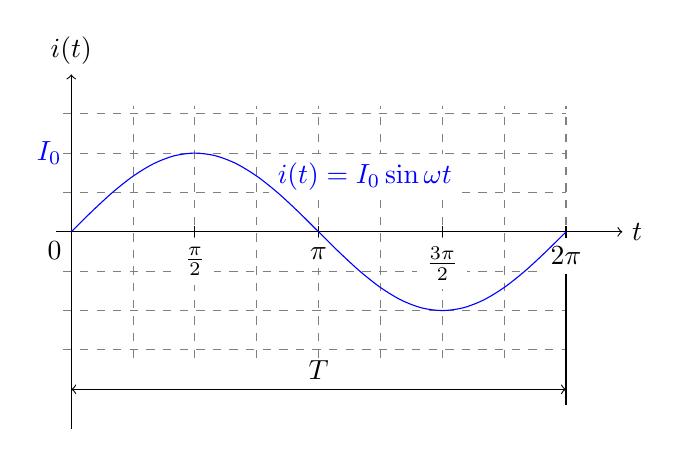
\begin{tikzpicture}[domain=0:2*pi] 
         \draw[xstep=pi/4, ystep=0.5, dashed, color=gray] (-0.1,-1.6) grid (2*pi,1.6); 
         \draw[->] (-0.2,0) -- (7,0) node[right] {$t$}; 
         \draw[->] (0,-2.5) -- (0,2) node[above] {$i(t)$}; 
         % text 
         \node[below left](0,0){$0$};
         \node[left, color=blue] at (0,1.0) {$I_0$}; 
         % period
         \draw[<->] (0,-2) -- (pi,-2) node[above]{$T$} --(2*pi,-2);
         \draw (2*pi,-2.2) -- (2*pi,0); 
         \foreach \x/\xtext in {0.5*pi/\frac{\pi}{2} ,pi/\pi, 1.5*pi/\frac{3\pi}{2}, 2*pi/2\pi}
         \draw[shift={(\x,0)}] (0pt,2pt) -- (0pt,-2pt) node[below, fill=white] {$\xtext$};  
         \node[below right, color=blue, fill=white] at (2.5,1.0) {$i(t) = I_0\sin\omega t$};
         % function 
         \draw[color=blue, smooth]   plot (\x,{sin(\x r)}); 
       \end{tikzpicture}  
       \captionsetup{type=figure}   
       \captionof{figure}{}\label{MA:fig_Iav_exam}
    \par}
  
%\end{document}  
    %----------------------------------

    Podle \ref{MA:eq_av2} bude
    \begin{align*}
     i_s &=  \frac{2}{T}
             \int_0^{\frac{T}{2}}I_0\sin\omega t\dd{t} =
             \frac{2I_0}{T}\left[-\frac{\cos\omega t}{\omega}\right]_0^{\frac{T}{2}}        \\
         &=  \frac{2I_0}{T}\frac{1}{\omega}\left(-\cos\frac{\omega T}{2}+ \cos 0\right)     \\
         &=  \frac{2I_0}{2\pi}(-\cos\pi + \cos 0) = \frac{2}{\pi}I_0 \doteq 0,637 I_0.
  \end{align*}

  Tato hodnota se rovná intenzitě elektrického proudu, při kterém by vodičem v průběhu uvažované
  poloviny periody prošel stejný elektrický náboj jako při proudu střídavém.
  \end{example}

  \begin{example} Efektivní hodnota $i_{ef}$ střídavého proudu $$i(t) = I_0\sin\omega t$$ (viz
    předchozí příklad) je definována jako odmocnina ze střední hodnoty funkce $i^2(t)$ v průběhu
    jedné periody $T = \frac{2\pi}{\omega}$. Tedy
    \begin{align*}
      i_{ef}^2 &= \frac{1}{T}\int_0^T I_0^2\sin^2\omega t\dd{t} = 
                  \frac{1}{T}\int_0^T \frac{I_0^2}{2}(1- \cos2\omega t)\dd{t}           \\
               &= \frac{I_0^2}{2T}
                  \left[
                    t-\frac{\sin2\omega t}{2\omega}
                  \right]_0^T = \frac{I_0^2}{2}
    \end{align*}
    neboť $\sin2\omega T=\sin4\pi = 0.$ Odtud $$i_{ef} = \frac{I_0}{\sqrt{2}}.$$ Střídavý proud
    $i(t) = I_0\sin\omega t$ má na témže odporu stejný výkon jako stejnosměrný proud o intenzitě
    $i = 0,707I_0$.
  \end{example}
  Následující věta může být využita k odhadu některých integrálů
  \begin{lemma}
    \textbf{Druhá věta o střední hodnotě integrálního počtu}: Jsou-li funkce $f(x)$ a $g(x)$
    spojité v intervalu $\langle a, b \rangle$ a je-li funkce $g(x)$ v $\langle a, b \rangle$
    nezáporná a nerostoucí, existuje alespoň jeden bod $c\in\langle a, b \rangle$ tak, že platí
    \begin{equation}\label{MA_eq_av3}
        \int_a^b f(x)g(x) = g(a)\int_a^c f(x)dx.
    \end{equation}
  \end{lemma}
  Zcela obdobnou větu lze vyslovit pro případ, že $g(x)$ je v intervalu $\langle a, b \rangle$
  nezáporná a neklesající, tj. na pravé straně \ref{MA_eq_av3} je pak integrál $g(b)\int_c^b
  f(x)dx$

  \begin{example} Odhadněte hodnotu integrálu
    \begin{equation}\label{MA_eq_sinx_x}
        \int_{100\pi}^{1000\pi}\frac{\sin x}{x}dx
    \end{equation}
    Řešení: Funkce $f(x) = \sin x$ a $g(x) = \frac{1}{x}$ jsou v uvažovaném intervalu $\langle
    100\pi, 1000\pi \rangle$ spojité a funkce $g(x)$ je kladná a nerostoucí.
    \begin{equation*}
      \int_{100\pi}^{1000\pi}\frac{\sin x}{x}dx = 
      \frac{1}{100\pi}\int_{100\pi}^c\sin xdx =\frac{1}{100\pi}\left(\cos100\pi - \cos c\right)
    \end{equation*}
    kde $c$ je kladné číslo z intervalu $\langle 100\pi, 1000\pi \rangle$. Dále pro všechna
    $c\in\langle 100\pi, 1000\pi \rangle$ platí $0\leq1-\cos c\leq2$, takže
    \begin{equation*}
        0\leq\int_{100\pi}^{1000\pi}\frac{\sin x}{x}dx\leq \frac{1}{50\pi}.
    \end{equation*}
  \end{example}   
%---------------------------------------------------------------------------------------------------
\printbibliography[heading=subbibliography]
\addcontentsline{toc}{section}{Seznam literatury}
%  \input{../src/MAI/chapters/Series.tex}
%  % !TeX spellcheck = cs_CZ
{\tikzset{external/prefix={tikz/MAI/}}
 \tikzset{external/figure name/.add={ch09_}{}}
%---------------------------------------------------------------------------------------------------
% file ODR.tex
%---------------------------------------------------------------------------------------------------
\chapter{Obyčejné diferenciální rovnice}
\minitoc
%================Kapitola: Diferenciální rovnice 1. řádu ===========================================
  \section{Diferenciální rovnice 1. řádu}
    Řada fyzikálních principů má tvar výroku, resp. vztahu mezi jistými veličinami (funkcemi) a
    jejich změnami, vztaženými ke zvoleným nezávisle proměnným pa\-ra\-me\-trům (čas, souřadnice).
    Změny (okamžité, lokální) se nejlépe vystihují pomocí derivací. Takový zákon má pak charakter
    vztahu mezi uvažovanými veličinami a jejich derivacemi. Nejčastěji bývá vztah vyjádřen formou
    rovnosti:
    \begin{itemize}
   	  \item Newtonůw zákon: okamžitá změna hybnosti $p(t) = m(t)\cdot v(t)$ pohybujícího se
         	objektu je úměrná působící síle $F(t)$ v každém okamžiku $t$ zvoleného časového rozmezí
        	$$\frac{d}{dt}\left(m(t)\cdot v(t)\right) = F(t)\quad t\in\langle\alpha, \beta\rangle$$
      \item Kirchhoffův zákon pro LR – obvod: v okamžiku $t$ je součet napětí na cívce s indukčnosti
            $L$ a na rezistoru o odporu $R$ roven napětí $U(t)$ na svorkách zdroje. Tuto rovnost pak
            zapisujeme ve tvaru (pro L,R = konst)
            \begin{equation}
              L\frac{di(t)}{dt}+Ri=u(t), 
            \end{equation}
            kde $i=i(t)\ldots$ funkce popisující závislost proudu na čase.
    \end{itemize}
    
    Chceme-li určit funkci $i=i(t)$ popisující průběh proudu v obvodu tak, aby byl splněn příslušný
    K.z. a současně, aby byl splněn požadavek na počáteční stav:
    \begin{equation}
        L\frac{di(t)}{dt}+Ri(t)=U,\quad i(0)=I_0,\quad t\in\langle 0,+\infty)
    \end{equation}
    Metodami uvedenými později stanovíme právě jednu funkci $i=i(t)$, která je řešením dané tzv.
    \textbf{počáteční úlohy}.
    \begin{equation}
      \begin{array}{c}
         i(t)=I_0\left(1-e^{-\frac{R}{L}t}\right),\quad t\in\langle 0,+\infty), \\
         lim_{t\rightarrow +\infty}i(t)=\frac{U_0}{R},\quad lim_{t\rightarrow +0}i(t)=I_0=i(0)
      \end{array}
    \end{equation}
    \begin{itemize}
      \item tedy obvykle formulujeme úlohu najít jistou funkci tak, aby zákon byl splněn tj.
            Kirchhoffův zákon užijeme k tomu, abychom nalezli funkci $i(t)$
      \item užijeme-li rovnosti vyjadřující takový zákon k tomu, abychom určili funkci, která v
            takovém vztahu vystupuje spolu s derivacemi, stává se tento požadavek úlohou, která má
            charakter rovnice s derivacemi, neboli diferenciální rovnice. Funkce, která požadavek
            splňuje, se pak nazývá řešení diferenciální rovnice.
    \end{itemize}
    
    \begin{figure}
      \centering
      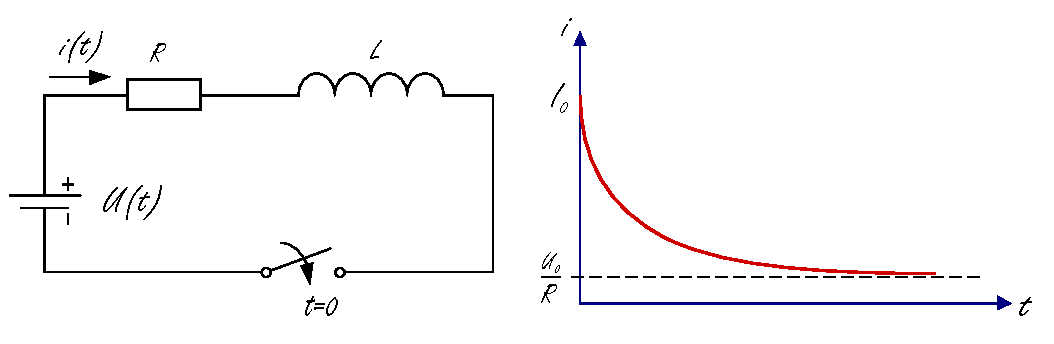
\includegraphics[width=\linewidth]{motivace.pdf}
      \caption{Graf průběhu proudu $i(t)$ po sepnutí spínače v době $t=0$.}
      \label{figure:odr_motivace}
    \end{figure}

} %tikzset
%---------------------------------------------------------------------------------------------------
%\printbibliography[heading=subbibliography]
\addcontentsline{toc}{section}{Seznam literatury}
%  % !TeX spellcheck = cs_CZ
{\tikzset{external/prefix={tikz/MAI/}}
 \tikzset{external/figure name/.add={ch10_}{}}
%---------------------------------------------------------------------------------------------------
% file ppst.tex
%---------------------------------------------------------------------------------------------------
\chapter{Počet Pravděpodobnosti}
\minitoc
  Slovo pravděpodobnost používáme velmi často. Jaký však je jeho přesný význam? Jsme přesvědčeni, 
  že pravděpodobnost výhry ve sportce je velmi malá. Ani pravděpodobnost, že se vyplní předpověď 
  počasí, nepovažujeme mnohdy za výraznou. Přesto je mezi oběma příklady obrovský kvantitativní 
  rozdíl. Zkusme význam pojmu pravděpodobnost ukázat pomocí konkrétních číselných příkladů.
  
  \begin{itemize}
    \item \textbf{Příklad se střelcem}: Sportovní střelec střílí na terč série \num{100} ran. 
          Předpokládejme, že podmínky při střelbě jsou stále stejné. Stejná je zbraň, terč, 
          vzdálenost, povětrnostní podmínky i momentální zdravotní stav střelce Při hodnocení 
          střelcova „mistrovství“ někdo řekne, že střelec zasáhne terč s pravděpodobností 
          \num{92}\%. Jak tomu rozumět? Znamená to, že v souboru sérií výstřelů jsou velmi časté 
          ty, v nichž zasáhl střelec terč \num{92}-krát. Samozřejmě, není řídké, že se objeví i 
          série s \num{93} nebo \num{94} zásahy, ale také s \num{91} nebo \num{90}. Vyloučen není 
          ani případ s úspěšností \num{96} či \num{88}, a dokonce i stovku bychom mohli zaznamenat. 
          Situace výrazně odlišné od \num{92} zásahů však budou řídké, a to tím více, čím více se 
          úspěšnost série liší od \num{92} oběma směry.
    \item \textbf{Příklad se zmetky}: Koupíte si výrobek u firmy, o které je známo, že vyrábí 
          zmetky s pravděpodobností 0,16\%? Situaci lze posuzovat obdobně jako úspěšnost střelce. 
          Budeme-li například zkoumat série obsahující 1000 výrobků, bude každá z nich obsahovat „v 
          průměru“ 16\% zmetků. Z příkladu se střelcem již zhruba víme, jak posuzovat slovo v 
          průměru.
  \end{itemize}
  
  V této kapitole se budeme pravděpodobnostmi zabývat podrobněji. Zjistíme, že i když se týkají 
  náhodných jevů, platí i pro ně jisté zákonitosti.
    
  \section{Pravděpodobnost}
    V úvodních příkladech jsme si vyložili, jak intuitivně chápat pojem pravděpodobnost. Jednalo se 
    v nich o posouzení průměrné úspěšnosti ve velkém souboru operací či úkonů prováděných za 
    stejných podmínek, šlo tedy o jakousi „průměrnou“ pravděpodobnost. Nyní definujeme 
    pravděpodobnost matematicky.
    
    \subsection{Co se pravdě podobá — definice pravděpodobnosti}
      Pro definici pravděpodobnosti použijeme pojmu \emph{náhodný pokus}, jehož význam si ukážeme 
      na příkladu. Dobrým příkladem náhodných pokusů je třeba házení mincí, hraní kostkou, výběr 
      karet z balíčku, vidíme-li pouze jejich rub, apod. Budeme třeba házet kostkou. Abychom si 
      situaci zbytečně nekomplikovali, budeme předpokládat, že všechny výsledky hodu kostkou 
      (náhodné pokusy) jsou stejně časté, žádný z nich není nijak preferován\footnote{Kostka by 
      tedy měla být homogenní, plocha, na kterou po hodu dopadne, vodorovná, kvalita povrchu všech 
      stěn kostky stejná (žádná stěna by třeba neměla být natřena lepidlem), apod.}. Počet možných 
      výsledků jednotlivého hodu je \(N = 6\) (kostka má \num{6} stěn, na každé je vyznačen odlišný 
      počet ok, tedy \num{1} až \num{6}). Jednotlivé situace, které mohou nastat, nazýváme 
      náhodnými jevy. Náhodným jevem \(A\) tak může být situace \emph{„padne číslo \num{2}“}, jiným 
      náhodným jevem \(B\) situace \emph{„padne číslo dělitelné třemi“}, apod. Počet situací, kdy 
      výsledek hodu lze hodnotit tak, že určitý jev nastal, označíme \(M\). Například pro jev \(A\) 
      \emph{„padne číslo \num{2}“} je \(M(A)= 1\), pro jev \(B\) \emph{„padne číslo dělitelné 
      třemi“} je \(M(B) = 2\) (počet ok \num{3} nebo \num{6}). Můžeme také definovat jev \(O\) 
      \emph{„nepadne žádné číslo“} (\(M(0) = 0\)) nebo jev \(J\) \emph{„padne jakékoli číslo“} 
      (\(M(J) = 6\)).
      
      \begin{definition}
        Pravděpodobností jevu rozumíme podíl
        \begin{equation}\label{mai:eq011}
          p = \frac{M}{N} = \frac{\text{počet případů příznivých}}{\text{počet případů možných}}.
        \end{equation}  
        Počtem případů možných jsme zkráceně nazvali počet všech možných výsledků náhodného 
        pokusu, počtem případů příznivých pak počet všech takových výsledků pokusu, při nichž daný 
        jev nastal.
      \end{definition}
      Je zřejmé, že hodnota pravděpodobnosti jakéhokoli jevu je nezáporná a může nabývat hodnoty 
      nejvýše \num{1}, tj. \(0 <p< 1\). Jev s \emph{nulovou pravděpodobností} se nazývá 
      \textbf{nemožný}, jev s \emph{jednotkovou pravděpodobností} je \textbf{jistý}. V našem 
      příkladu s kostkou tak dostáváme
      \begin{equation*}
        p(A) = \frac{1}{6}, \qquad p(B) = \frac{2}{6} = \frac{1}{3}, \qquad
        p(O) = 0, \qquad p(J) = 1.
      \end{equation*}  

      %---------------------------------------------------------------
      % !TeX spellcheck = cs_CZ
\begin{example}
 \label{mai:exam006}
  \textbf{Barevné ponožky}:\newline
  V zásuvce jsou ponožky tří barev. Červené (\textbf{Č}), zelené (\textbf{Z}) a modré (\textbf{M}). 
  Je jich tam od každé barvy hodně. Student jde na schůzku a chce si vzít čisté ponožky. Náhle 
  zhasne světlo. Student vytáhne potmě dvě ponožky. Jaká je pravděpodobnost, že ponožky budou mít 
  stejnou barvu? Vyjmenujme případy, které mohou při vytažení dvou ponožek nastat: (\textbf{Č+Č}), 
  (\textbf{Č+Z}), (\textbf{Z+Č}), (\textbf{Č+M}), (\textbf{M+Č}), (\textbf{Z+Z}), (\textbf{Z+M}), 
  (\textbf{M+Z}), (\textbf{M+M}). Je tedy \(n = 9\). Příznivé situace jsou tří, (\textbf{0+0}), 
  (\textbf{Z+Z}), (\textbf{M+M}). Pravděpodobnost je tedy 1/3.  
\end{example}
      %---------------------------------------------------------------
    \subsection{Cifry, kostky, karty - kombinatorické opakování}
      Příklad s ponožkami byl velmi jednoduchý. Podařilo se nám vyjmenovat všechny případy možné i 
      všechny případy příznivé, neboť obojího bylo docela málo. Daleko běžnější jsou však situace, 
      kdy výčet případů není schůdný. A tehdy potřebujeme \textbf{kombinatoriku}.
      
      Nechť \(\mathcal{M}\) je \(n\)-prvková množina, z níž budeme provádět výběry \(k\) prvků 
      podle určitých pravidel. Prvky množiny \(\mathcal{M}\) nemusíme nijak konkretizovat. Abychom 
      si však o výběrech a pravidlech pro jejich tvorbu dokázali udělat nějakou názornou představu, 
      je taková konkretizace vhodná. Prvky množiny \(\mathcal{M}\): mohou být třeba žáci ve třídě, 
      barvy, hrací karty, apod. Výběry mohou představovat třeba družstva pro odbíjenou, signály 
      tvořené barevnými praporky, možnosti rozdání karet při mariáši, apod. Jednotlivé typy výběrů 
      získaly své názvy právě na základě pravidel stanovených pro jejich vytváření. Rozhodující 
      jsou dvě základní kritéria:
      \begin{itemize}\addtolength{\itemsep}{-0.5\baselineskip}
        \item Je pro tvorbu výběru podstatné pořadí prvků ve výběru či nikoliv?
        \item Mohou se prvky ve výběru opakovat či nikoliv?
      \end{itemize}
      
      Typy výběrů shrnuje následující diagram:
      \begin{figure}[ht!] %\ref{mai_fig021}
        \centering
        \begin{tikzpicture}[scale=0.8, every node/.style={transform shape},
    node distance = 6mm and 6mm,
    start chain = going below,% <-- new
    base/.style = {draw, minimum width=4.5em, align=flush center, outer sep=0pt,
                       on chain},% <-- new
    decision/.style = {shape=signal, base,% <-- new, replace diamond
                       signal to=west and east,
                       top color=white, bottom color=green!50!black!50},
    process/.style = {shape=rectangle, base,
                       top color=white, bottom color=blue!50!black!50},
    startstop/.style = {shape=rectangle, base,
                       rounded corners,
                       top color=white, bottom color=red!30},
    arrow/.style = {thick, -stealth},
    every join/.style = {arrow}
                          ]
% left column 
    \node (1) [decision, bottom color=red!50!black!50] {Pořadí \\ rozhoduje};
    \node (2) [decision, left=of 1] {Opakování \\ prvků};
    \node (3) [process,join]  {Kombinace \\ bez opakování};
    \node (4) [process]  {Kombinace \\ s opakováním};
    \node (5) [decision, right=of 1] {Opakování \\ prvků};
    \node (6) [process, join] {Variace bez\\ opakování};
    \node (7) [process] {Variace s\\ opakováním};
\coordinate[left =of 2.west] (10);
\coordinate[right=of 5.east] (11);
% connection lines
\draw [arrow]   (1) edge ["ne"]   (2) 
                (1) edge ["ano"]  (5)
                (2) edge ["ne"]   (3)
                (5) edge ["ne"]   (6)
                (5)  to  ["ano"]  (11) |- (7);
\draw           (2)  to  ["ano"]  (10) |- (4);
\end{tikzpicture}
        \caption{Typy výběrů. \cite[s.~201]{Musilova2009MA1}}
        \label{mai_fig021}
      \end{figure}

      Představuje-li daný výběr například volejbalové družstvo osmi děvčat (šest hráček a dvě 
      náhradnice), které bude reprezentovat v soutěži třídu osmou bé, do níž chodí \num{25} děvčat 
      a \num{18} chlapců, jedná se o výběr \(k — 8\) prvků z počtu \(n = 25\) prvků. Chlapce nelze 
      postavit do družstva volejbalistek. Každý výběr možného družstva bude představovat 
      \emph{kombinaci bez opakování}, neboť pořadí hráček nehraje roli a třeba Aničku Novákovou 
      máme ve třídě jen jednu. Budeme-li však chtít vytvářet z deseti cifer \(0, 1, \ldots, 9\) 
      trojciferná čísla, pak tyto výběry tří prvků z deseti (\(k = 3\), \(n = 10\)) jsou 
      \emph{variacemi s opakováním}. Čísla \num{125}, \num{512}, \num{251}, \num{215}, \num{521} a 
      \num{152} jsou totiž různá, a například \num{222} je také trojciferné číslo. Kombinace s 
      opakováním bychom mohli vytvářet třeba i při výběru různobarevných ponožek ze zásuvky a 
      konečně \emph{variacemi bez opakování} by mohly být dejme tomu trojbarevné signály (\(k = 
      3\)) tvořené trojicemi barevných hadříků vybíraných z \(n\) barev (pro \(n = 3\) třeba zrovna 
      z těch ponožek). Nyní bychom však rádi věděli, jak pro zadané hodnoty \(n\) a \(k\) určit 
      počet všech možných výběrů předepsaného typu. Ukážeme si to na příkladech.

      %---------------------------------------------------------------
      % !TeX spellcheck = cs_CZ
\begin{example}\label{mai:exam007}
  \textbf{Šance milion}:\newline
  „Znáte nějakou jinou hru, kde můžete denně vyhrát milion?“ Tento nebo jiný, obdobně nepříliš 
  vtipný reklamní slogan propaguje v televizi hru, jejímž cílem je uhodnout šestici tažených cifer 
  ve správném pořadí. (Hru raději nehrajte, pravděpodobnost výhry je mizivá.) Tah se provádí 
  následovně: V každém ze šesti bubnů, očíslovaných pořadovými čísly \num{1} až \num{6}, je 
  připraveno deset míčků opatřených ciframi \(0, 1, \ldots, 9\). Z prvního bubnu se náhodně 
  vylosuje jedna cifra (deset možností). Poté se náhodně vylosuje jedna cifra z druhého bubnu (opět 
  deset možností). Možností vzniku uspořádané dvojice cifer (jedna cifra z prvního a druhá z 
  druhého bubnu) je již sto (každou možnost výsledku u prvního bubnu lze kombinovat s každou 
  možností výsledku z druhého bubnu). Losování pokračuje u třetího, čtvrtého, pátého a šestého 
  bubnu. Celkový počet možností je \num{1e6}, tedy \textbf{milion}. (Šance získat výhru, tedy 
  vyhrát milion, je ovšem pouze jedna milióntina, neboť z milionu možností je pouze jedna skutečně 
  tažena.) 
\end{example}
      %---------------------------------------------------------------
      
      Zobecněním předchozího příkladu získáváme vzorec pro počet \textbf{variací s opakováním} 
      \emph{k}-té třídy z \(n\) prvků. Při tahu totiž záleží na pořadí bubnů a každý buben obsahuje 
      všechny cifry. Výsledky tahů z jednotlivých bubnů se tedy mohou opakovat. Pokud by bubnů bylo 
      \(k\) a v každém \(n\) různých cifer, dostali bychom pro \textbf{variace s opakováním 
      \(k\)-té třídy z \(n\) prvků} celkový počet
      \begin{equation}\label{mai:eq007}
        \boxed{V_k' = n^k}\, .
      \end{equation}

      %---------------------------------------------------------------
      % !TeX spellcheck = cs_CZ
\begin{example}\label{mai:exam008}
  \textbf{Modifikovaná šance milion}:\newline
  Představme si hru z předchozího příkladu upravenou takto: K dispozici bude jen jeden buben s 
  ciframi \(0, 1, \ldots, 9\), každá cifra je v bubnu obsažena pouze jednou. Opět máme losovat 
  uspořádanou \textbf{šestici cifer}. Nyní se však jedná o \textbf{variace šesté třídy z deseti 
  prvků bez opakování}. S jediným bubnem musíme totiž provést šest losování, přičemž při každém 
  losování ubude z bubnu jedna cifra. Při prvním tahu je deset možností, při druhém již jen devět, 
  atd., při šestém již pouze pět možností. Celkem je tedy \(10 \cdot 9 \cdots 5 = \num{151200}\) 
  možností.
\end{example}
      %---------------------------------------------------------------
      
      Uvážíme-li, že v předchozím příkladu je \(n = 10\) a \(k = 6\), dostáváme pro \textbf{počet 
      variací bez opakování \(k\)-té třídy z \(n\) prvků} obecný vztah
      \begin{align}
        V_k(n) &= n(n-1)(n-2)\cdots(n-k+1)  \nonumber \\
        \shortintertext{neboli}
        V_k(n) &= \frac{n!}{(n-k)!}\, .    \label{mai:eq008}
      \end{align}
      Poznamenejme, že \(n!\) značí \textbf{faktoriál}, \(n! = n(n — 1)\cdots 3 \cdot 2 \cdot 1\). 
      Pro nulu definujeme \(0! = 1\). Je zřejmé, že při vytváření variací bez opakování musí být 
      \(k\leqq n\). Variace bez opakování \(n\)-té třídy z \(n\) prvků se nazývají 
      \textbf{permutace}. Každá z nich představuje určité uspořádání těchto \(n\) prvků. Platí
      \begin{equation}\label{mai:eq009}
        \boxed{P(n) = V_n(n) = n!}\, .
      \end{equation}
      
      Nyní odvodíme vzorec pro počet \textbf{kombinací \(k\)-té třídy z \(n\) prvků bez opakování}. 
      Již jsme si řekli, že \emph{kombinací} rozumíme takový výběr z celkového počtu \(n\) prvků, 
      který obsahuje určitých \(k\) prvků nezávisle na jejich pořadí. Představme si, že máme k 
      dispozici všechny variace bez opakování \(k\)-té třídy ze zmíněných \(n\) prvků. Vezměme 
      kteroukoli z nich. Soubor všech variací \(k\)-té třídy z \(n\) prvků však obsahuje i další 
      variace, lišící se od té naší jen pořadím prvků. Celkem je takových variací (i s tou první) 
      \(k!\) a z hlediska kombinací představují totéž. Soubor variací se tak rozpadá na podsoubory, 
      z nichž každý obsahuje \(k!\) variací lišících se navzájem pouze pořadím prvků. Každý z 
      těchto podsouborů představuje však jedinou kombinaci. Počet kombinací \(k\)-té třídy z \(n\) 
      prvků bez opakování je tedy
      \begin{equation}\label{mai:eq010}
        \boxed{C(k) = \frac{V_k(n)}{P(k)} = \frac{n!}{(n-k)!\,k!} = 
               \begin{pmatrix}
                n \\
                k
               \end{pmatrix}}\, .
      \end{equation}
      
      Pro odvození vzorce pro \textbf{kombinace s opakováním} použijeme opět příkladu.
      %---------------------------------------------------------------
      % !TeX spellcheck = cs_CZ
\begin{example}\label{mai:exam009}
  \textbf{Kuličky v přihrádkách}:\newline
  Máme kuličky \(n\) různých barev, v každé barvě máme tolik kuliček, kolik bude potřeba. Naším 
  úkolem je vytvářet výběry \(k\) kuliček. Na \textbf{pořadí barev nezáleží}, kuliček jedné barvy 
  může být ve výběru libovolný počet \(0\leqq s \leqq k\). Výběry budeme vytvářet tak, že budeme 
  kuličky dávat do \(n\) přihrádek, z nichž každá bude vyhrazena pro určitou barvu. Pokud tedy v 
  daném výběru zrovna nebude třeba modrá kulička, bude přihrádka vyhrazená pro modrou barvu 
  prázdná. Budou-li v daném výběru právě tři červené kuličky, budou umístěny v přihrádce vyhrazené 
  pro červenou barvu. Vidíme, že pokud konkrétním přihrádkám přisoudíme konkrétní barvy, samotné 
  kuličky by již barevné být nemusely, stačily by třeba kuličky skleněné, bezbarvé. Zůstane-li 
  například přihrádka pro modrou barvu prázdná, víme, že daný výběr neobsahuje modrou barvu. 
  Budou-li v přihrádce pro červenou barvu tři (bezbarvé) kuličky, víme, že daný výběr obsahuje 
  červenou barvu třikrát. Příklad takové situace ukazuje následující schéma:
  
  {\centering
    
\includegraphics[width=0.5\linewidth]{MAI014.pdf}
    \par}

  Náš úkol můžeme přeformulovat takto: Je třeba rozmístit \(k\) kuliček do \(n\) přihrádek. V každé 
  přihrádce může být obecně \(s\) kuliček, kde \(0\leqq s \leqq k\), přitom celkový počet kuliček 
  musí být samozřejmě stále \(k\). Můžeme si představit, že \(k\) kuliček máme položených v řadě na 
  polici mezi dvěma pevnými stěnami (krajní svislé čáry v předchozím schématu) a různé způsoby 
  rozmístění kuliček do přihrádek provádíme přemísťováním pohyblivých přepážek. Kdybychom například 
  v předchozím schématu přesunuli druhou svislou čáru, počítáno zleva, až za první kuličku v 
  přihrádce na červenou barvu, dostaneme uspořádání, při němž je v přihrádce na modrou barvu jedna 
  kulička a v přihrádce na červenou barvu dvě kuličky. Tedy takto:

  {\centering
    
\includegraphics[width=0.5\linewidth]{MAI015.pdf}
    \par}

  Mezi dvěma krajními pevnými stěnami máme tedy k dispozici \(k\) pozic pro kuličky a \((n — 1)\) 
  pozic pro pohyblivé přepážky. Celkem tedy \((n + k — 1)\) pozic, na které můžeme libovolně 
  rozmísťovat \(k\) kuliček a \((n — 1)\) přepážek. Do těchto \((n + k — 1)\) pozic můžeme umístit 
  \(k\) kuliček \(C_k'(n)\) způsoby, kde
  
  \begin{equation}\label{MAI:eq011}
  \boxed{C_k'(n) =  
    \begin{pmatrix}
        n + k - 1 \\
        k
    \end{pmatrix} = 
    \begin{pmatrix}
        n + k - 1 \\
        n-1
    \end{pmatrix}
    }\, .
  \end{equation}
  Na zbylé pozice již musíme umístit přepážky. Nebo naopak, nejprve umístíme \((n — 1)\) přepážek a 
  potom kuličky. Výsledek je stejný, jak je vidět z předchozího vzorce. Protože jsme vytváření 
  kombinací s opakováním \(k\)-té třídy z \(n\) prvků převedli na úlohu o rozmísťování kuliček do 
  přihrádek, udává získaný vzorec právě počet takových kombinací. Aby měl vzorec smysl, musí platit 
  \(n + k — 1 \geqq k\), tedy \(n \geqq 1\).
  
\end{example}
      %---------------------------------------------------------------
      
      Komu nevyhovuje představa kuliček v přihrádkách a má raději čísla, může uvažovat následovně: 
      Tak jako je každé číslo v desítkové soustavě zapsáno pomocí cifer \(0, 1, 2, \ldots , 8, 9\), 
      je k jeho zápisu ve dvojkové soustavě potřeba pouze dvou cifer, nuly a jedničky. Představme 
      si nyní přepážku jako jedničku a kuličku jako nulu. Náš úkol zjistit počet všech možných 
      způsobů rozdělení \(k\) kuliček do \(n\) přihrádek, ohraničených \((n+1)\) přepážkami, můžeme 
      převést na ekvivalentní problém: Kolik dokážeme najít čísel, která jsou ve dvojkové soustavě 
      zapsána právě \(k\) nulami a \((n + 1)\) jedničkami, požadujeme-li, aby první i poslední 
      cifrou byla jednička? Odpověď je jednoduchá. Máme k dispozici \((n+k+1)\) pozic pro cifry. 
      První a poslední pozice jsou pevně obsazeny jedničkami, volných pozic je tedy pouze \((n + k 
      — 1)\). Počet všech různých způsobů, kterými na \(k\) z těchto pozic můžeme umístit nuly, je 
      roven počtu kombinací \(k\)-té třídy z \((n + k — 1)\) prvků. Na zbylé pozice již musíme 
      umístit jedničky. Komplementárně, budeme-li hledat počet všech možných způsobů, jak na 
      \((n—1)\) pozic umístit jedničky, dostaneme shodný výsledek, v souhlasu se vzorcem 
      (\ref{mai:eq010}).
      
      %---------------------------------------------------------------
      % !TeX spellcheck = cs_CZ
\begin{example}\label{mai:exam010}
  \textbf{Obsazování kvantových stavů}:\newline
  Úloha o kuličkách a přihrádkách má přímou aplikaci v \textbf{kvantové fyzice}. Představme si, že 
  fyzikální soustava je tvořena \(K\) částicemi. Každá částice se nachází v určitém stavu, v němž 
  jí můžeme přisoudit fyzikální charakteristiky, které jsou s tímto stavem spojeny (třeba energii, 
  moment hybnosti, apod.). Jednotlivé stavy jsou pak rozlišitelné právě pomocí těchto 
  charakteristik. Dejme tomu, že přípustných stavů je \(n \geqq 1\). Problémem kvantové fyziky je 
  to, že kvantové částice jsou nerozlišitelné. Nepoznáme jednu od druhé. Je to stejné, jako bychom 
  měli \(k\) naprosto stejně vypadajících kuliček, které nemáme nijak očíslovány. Záměna dvou 
  částic (nerozlišitelných kuliček) se nepozná, nevede tedy ke změně stavu fyzikální soustavy. Pro 
  hodnoty fyzikálních charakteristik soustavy jako celku je tedy důležité jen to, kolik částic je v 
  každém z přípustných stavů. Musíme se tedy zajímat o to, kolika způsoby lze našich \(k\) 
  \textbf{nerozlišitelných částic} (kuliček) umístit do \(n\) \textbf{stavů} (přihrádek). Kvantové 
  částice jsou však dvojího druhu, \textbf{fermiony} (například elektrony, neutrony, protony, jádra 
  s lichým počtem nukleonů) a \textbf{bosony} (například fotony, mezony, jádra se sudým počtem 
  nukleonů). Rozdíl mezi nimi je ten, že bosony se „dobře snášejí“, a proto jich může být v jednom 
  stavu i více. 
  \begin{itemize}\addtolength{\itemsep}{-0.5\baselineskip}
    \item Počet možností, jak rozmístit \(k\) \textbf{bosonů} po \(n\) stavech je tedy
          \begin{equation*}
            N_{\text{boson}} = 
              \begin{pmatrix}
                n + k - 1 \\
                    k
               \end{pmatrix}
          \end{equation*}
    \item S \textbf{fermiony} je tomu jinak. \textbf{Pauliho vylučovací princip} jim zakazuje, 
          aby v daném stavu byl více než jeden fermion. Stav může být buď prázdný, nebo obsazen 
          jedním fermionem. V takovém případě musí být \(n \geqq k\) a v každé přihrádce může být 
          nejvýše jedna kulička. Situace tak odpovídá \textbf{kombinacím bez opakování \(k\)-té 
          třídy z \(n\) prvků}, tj.
          \begin{equation*}
            N_{\text{fermion}} = 
              \begin{pmatrix}
                n  \\
                k
              \end{pmatrix}
          \end{equation*}
  \end{itemize}  
\end{example}
      %---------------------------------------------------------------
      
      Získané kombinatorické vzorce nyní použijeme při řešení základních úloh o pravděpodobnostech. 
      V každé úloze bude důležité
      \begin{itemize}
        \item definovat jev \(A\), jehož pravděpodobnost počítáme,
        \item určit počet \(N\) případů možných, tj. počet všech možných výsledků pokusu, při 
              kterém sledujeme, zda jev \(A\) nastal či nenastal,
        \item určit počet \(M\) případů příznivých, tj. počet těch výsledků daného pokusu, při 
              kterých jev \(A\) nastal.
      \end{itemize}
      
} %tikzset
%---------------------------------------------------------------------------------------------------
\printbibliography[heading=subbibliography]
\addcontentsline{toc}{section}{Seznam literatury}
%  % !TeX spellcheck = cs_CZ
{\tikzset{external/prefix={tikz/MAI/}}
 \tikzset{external/figure name/.add={ch11_}{}}
%---------------------------------------------------------------------------------------------------
% file NM.tex
%---------------------------------------------------------------------------------------------------
\chapter{Numerické metody}
\minitoc

  \section{Úvodní slovo}
    Numerické metody jsou metody, které na rozdíl od metod analytických poskytujících spojité řešení
    na určité předem definované oblasti, dávají čísel\-né řešení v předem zvolených diskrétních
    bodech této oblasti. Na rozdíl od analytických metod toto řešení většinou nebývá přesné, ale
    představuje pouze jeho aproximaci, která je zatížena určitou chybou.
    
    Možnosti analytických metod se již asi třicet let pokládají prakticky za vyčerpané. Drtivá
    většina problémů (a to zdaleka nejen v oblasti technických věd), které bylo možno analyticky
    vyřešit, již tehdy byla vyřešena. Při vyčíslování výsledků ovšem v mnoha případech nastávaly
    značné problémy; spojité řešení bylo například popsáno kombinací vyšších funkcí (Besselovy,
    Legendrovy atd.) v podobě nekonečných řad, přičemž bylo třeba načítat dostatečný počet jejich
    členů k dosažení požadované přesnosti. A zde se již začaly uplatňovat různé numerické techniky,
    které ovšem bylo v té době možno realizovat jen na kalkulačkách nebo ze současného pohledu na
    primitivních počítačích.
  
    Ačkoli základy sofistikovaných numerických metod byly položeny již před více než šedesáti lety,
    jejich intenzivní a široký rozvoj je spojen teprve s vývojem a zdokonalováním výpočetní techniky
    v posledních asi čtyřiceti letech a lze říci, že v poslední době s řešením čím dál tím
    složitějších problémů ze všech vědních oblastí (nestacionární a nelineární úlohy ve 2D a 3D)
    stále nabývají na významu.
  
    Výsledkem aplikace převážné většiny numerických metod je sestavení velkého systému lineárních či
    nelineárních algebraických rovnic, který je nutno nějakým způsobem vyřešit existují ovšem
    numerické techniky i pro jiné účely, jako je například součet různých řad, výpočet určitých
    integrálů atd., jejich počet však není příliš velký). A v popředí zájmu jsou především dvě
    otázky:
    \begin{itemize}
      \item jak sestavit onen systém tak, aby počet zmíněných rovnic byl co nej\-men\-ší (přičemž 
            ale informace o rozložení hledané veličiny v oblasti je maximální a co nejpřesnější) a
      \item jak tento systém vyřešit co nejrychleji a s nejmenší možnou chybou.
    \end{itemize}
    Na tomto místě je nutno podotknout, že i malá vylepšení stávajících postupů mohou při řešení
    složitých úloh vedoucích na řešení soustav milionů či desítek milionů rovnic (aktuální stav)
    zajistit velmi výrazné časové úspory. Samotná realizace jakékoli numerické metody sestává z
    několika kroků:
    \begin{itemize}
      \item Sestavení matematického modelu dané úlohy. Tento krok je sám o sobě často nesmírně
            komplikovaný; reálný fyzikální problém musíme mnohdy zjednodušit tak, aby byl vůbec
            dostupnými prostředky řešitel\-ný, aniž by však vzniklé chyby přesáhly přijatelné 
            hodnoty. Takový matematický model zpravidla sestává z různých rovnic (algebraických,
            diferenciálních, integrálních, smíšených), neurčitých nebo určitých integrálů a podobně.
      \item Výběr konkrétní metodiky, jakou tento model budeme řešit. Uvedená me\-to\-di\-ka by měla
            být co nejvýhodnější z celé řady hledisek, jako je rychlost výpočtu, spolehlivost,
            robustnost, přesnost, konvergence, stabilita atd. O těchto pojmech jistě už většinou 
            máme jakousi intuitivní představu, v dalším textu však některé z nich upřesníme. Na 
            základě zvolené metody vypracujeme algoritmus, což je konečné množství instrukcí, které 
            musíme provést, aby se celý výpočet bezezbytku provedl.
      \item Navržený algoritmus musíme nyní naprogramovat. Přitom lze využít buď nějakého
            programovacího jazyka (FORTRAN, C++ a další), nebo nějakého prostředí s již
            předprogramovanými operacemi nebo celými bloky výpočtů (MatLab, Mathematica). V 
            některých případech lze využít i již existujících profesionálních programů, které 
            takový algoritmus
            obsahují (freeware tohoto typu je velmi řídké). Ty jsou ovšem velmi drahé a uživatel do
            nich zpravidla nemůže zasahovat za účelem například optimalizace výpočtu.
      \item Dalším krokem je realizace výpočtu. Zde je kromě provedení samotného výpočtu nutné
            ověřit, že výsledky jsou korektní. K tomu používáme buď experiment, nebo jinou metodu,
            která je již pro úlohu daného typu spolehlivě prověřená. Dále ověřujeme celou řadu
            aspektů, jako je například geometrická konvergence řešení (závislost výsledků na hustotě
            diskretizační sítě) a popřípadě jiná kritéria, o nichž se více dozvíme později.
      \item Posledním krokem je vyhodnocení a posouzení získaných výsledků, zpravidla na vizuálním
            základě, porovnáním, ale i jinak.
    \end{itemize}
  
  \section{Reprezentace čísel ve výpočetní technice}
    Při realizaci numerických algoritmů na počítači se lze setkat se dvojí reprezentací čísel, a to
    pomocí \textbf{pevné} nebo \textbf{plovoucí desetinné tečky}. Pevná desetinná tečka znamená vždy
    předem definovaný počet desetinných míst. Pracujeme-li se čtyřmi desetinnými místy, interpretují
    se následující čísla takto:
  
    \begin{table}[h]
      \centering
        \begin{tabular}{l r}
          \hline
          8675             & 8675.0000  \\
          \quad  3.24      &    3.2400  \\
          \quad -0.000006  &   -0.0000  \\
          \hline
        \end{tabular}
        \caption{Reprezentace čísel v pevné desetinné tečce}
    \end{table}
  
    Zatímco první dvě čísla jsou zobrazena přesně, třetí číslo nikoli, je zaokrouhleno. Proto je
    tento způsob nepraktický, při vědeckotechnických výpočtech se neužívá a v dalším textu se jím už
    nebudeme zabývat.
  
    Daleko pružnější je proto počítání s plovoucí desetinnou tečkou, kdy se v každém čísle 
    respektuje předepsaný počet prvních číslic. V tomto případě se uvedená čísla zobrazují takto:
  
    \begin{table}[h]
      \centering
        \begin{tabular}{l c c l}
           \hline
           8675             & +0.8675E+04 & nebo & +8.675E+03  \\
           \quad  3.24      & +0.3240E+01 & nebo & +3.240E+00  \\
           \quad -0.000006  & -0.6000E-05 & nebo & -6.000E-06  \\
           \hline
        \end{tabular}
        \caption{Reprezentace čísel v plovoucí desetinné tečce}
    \end{table}
  
    Každé nenulové číslo a lze reprezentovat jako $a= +m\cdot10^e$ , kde $0.1 < m <1$ a $e$ je celé
    číslo. Samozřejmě, číslo $m$ může obsahovat nekonečnou řadu číslic a celé číslo $e$ se může
    pohybovat od minus nekonečna do nekonečna. To ale v počítačové reprezentaci není možné; zde je
    číslo $m$ omezeno na konečný počet $n$ číslic a právě tak je omezen i exponent. Číslo $a$ je 
    tedy počítačem aproximováno jako $a= \pm m\cdot10^e$, kde $m=0.d1d2\ldots dn$. Toto číslo $m$ se
    nazývá \textbf{mantisa} a $e$ \textbf{exponent}.
  
    V jednoduché přesnosti má v počítačích e velikost $|e|< 38$, ve dvojité přesnosti $|e|<308$.
    Jsou-li tyto hodnoty překročeny, vzniká chyba známá jako \textbf{underflow} nebo
    \textbf{overflow}.
  
    \subsection{Zaokrouhlování}
      Čísla jsou v počítačové interpretaci často zaokrouhlována (mají-li v mantise velký počet
      číslic), poněvadž mantisa $m$ zde může těchto číslic obsahovat pouze $n$. Pravidla
      zaokrouhlování jsou jasná. Zopakujeme zde jen to, že čísla typu 7.65 nebo 7.75 (chceme-li
      zrušit jedno desetinné místo) zaokrouhlíme tak, že poslední číslice je sudá. Takže zatímco 
      7.65 zaokrouhlíme na 7.6, 7.75 zaokrouhlíme na 7.8.
  
      Chybu při zaokrouhlování můžeme určit jako ($n$ je počet číslic v mantise $m$)
      \begin{equation}\label{nm:eq_err_round}
        |\frac{m-\underline{m}}{m}|\leq\frac{0.5}{10^{n-1}}
      \end{equation}  
  
  %============ Kapitola: Chyby při numerických výpočtech =========================================
  \section{Chyby při numerických výpočtech}
    Protože základem numerických metod je získávání přibližných výsledků, je nutné mít vždy
    představu, jaký rozdíl může být mezi přesným řešením dané úlohy a řešením získaným použitou
    numerickou metodou.
    \subsection{Zdroje a typy chyb}
      Pomineme-li jako zdroj chyb člověka dopouštějícího se omylů, můžeme chyby rozdělit na několik
      základních druhů.
      \begin{itemize}
        \item \textbf{Chyby matematického modelu} - vznikají nahrazením reálné fyzikální situace
              matematickým modelem. Může se jednat například o popis nějakého fyzikálního děje 
              pomocí diferenciální rovnice.
        \item \textbf{Chyby vstupních dat} - jsou způsobeny nepřesnostmi při měření fyzikálních
              veličin
        \item \textbf{Chyby numerické metody} - vznikají při náhradě původní matematické úlohy
              jednodušší numerickou. Často se jedná o náhradu nekonečného procesu procesem konečným,
              např. při výpočtu hodnoty některé elementární funkce pomocí součtu několika prvních
              členů její nekonečné Taylorovy řady nebo při aproximaci určitého integrálu souč\-tem
              konečného počtu funkčních hodnot. Odhad této chyby je důležitou součástí řešení každé
              numerické úlohy.
        \item \textbf{Chyby zaokrouhlovací} - vznikají tím, že při výpočtech pracujeme s čísly
              zaokrouhlenými na určitý, relativně nevelký počet míst. Tyto chyby se při výpočtu 
              mohou kumulovat, nebo navzájem rušit. Při vel\-kém počtu operací je posouzení jejich 
              vlivu velmi náročné.
      \end{itemize}
      
    \subsection{Definice chyb, šíření chyb při výpočtu}
      \subsection{Absolutní a relativní chyba}
        Je-li hodnota $\underline{c}$ aproximace přesné hodnoty $c$, je \textbf{absolutní chyba}
        definována jako $\varepsilon=c-\underline{c}$ a \textbf{relativní chyba}
        $\varepsilon_r=\frac{\varepsilon}{c},c\neq0$. Tato definice se může zdát neužitečná, 
        poněvadž $c$ neznáme. Lze-li však říci, že pokud se aproximace $\underline{c}$ blíží k $c$, 
        můžeme psát $\varepsilon_r=\frac{\varepsilon}{\underline{c}},\underline{c}\neq0$. Bohužel, 
        většinou neznáme ani hodnotu $\varepsilon$. Někdy však její hodnotu můžeme odhadnout vztahem
        $|\varepsilon|\leq\sigma$ a podobně lze odhadnout pro relativní chybu 
        $|\varepsilon_r|\leq\sigma_r$.
      \subsubsection{Šíření chyb}
        \emph{Meze absolutních chyb při sčítání a odečítání se rovnají součtu pří\-sluš\-ných mezí.
        Meze relativních chyb při násobení a dělení se rovnají součtu mezí jednotlivých relativních
        chyb}.
        \begin{itemize}
          \item Nechť  $|x_i-\hat{x}_i|=|\varepsilon_i|\leq\sigma_i,\quad i=1,\cdots,n$. Pak je
               \begin{equation}\label{nm:eq_sireni_abs_err}
                 |\sum_{i=1}^n{x_i-\hat{x}_i}|=|\sum_{i=1}^n{\varepsilon_i}|\leq\sum_{i=1}^n{\sigma_i}
               \end{equation}
  
          \item Nechť dále $|\frac{x_i-\hat{x}_i}{x_i}|=|\varepsilon_{ri}|\leq\sigma_{ri},\quad
                i=1,\cdots,n$. Pak je
  
               \begin{align*}\label{nm:eq_sireni_rel_err}
                 |\frac{\prod_{i=1}^n{x_i}-\prod_{i=1}^n{\hat{x}_i}}{\prod_{i=1}^n{x_i}}|      &=
                             |\frac{\prod_{i=1}^n{x_i}-\prod_{i=1}^n{x_i-\varepsilon_i}}
                             {\prod_{i=1}^n{x_i}}|\doteq                                            
                             \\  
                 |\frac{\sum_{i=1}^n{\varepsilon_i}\prod_{j=1,j\neq i}^n{x_j}}
                             {\prod_{i=1}^n{x_i}}|                                             &=
                             |\sum_{i=1}^n{\frac{\varepsilon_i}{x_i}}|                              
                             \\
                 |\sum_{i=1}^n{\varepsilon_{ri}}|                                              &\leq
                             |\sum_{i=1}^n{\sigma_{ri}}|
              \end{align*}
        \end{itemize}
        kde jsme ale při rozdílu součinů v druhém výrazu zanedbali všechny násobky různých
        absolutních chyb, tedy členy druhého a vyšších řádů.
  
      \subsubsection{Podmíněnost numerických úloh a numerická stabilita algoritmů}
        Při numerickém řešení různých úloh musíme zkoumat, jaký vliv na výsledek mají malé změny ve
        vstupních hodnotách a zaokrouhlování během výpočtu. Řešení numerických úloh můžeme považovat
        za postup, kterým přiřazujeme vstupním údajům výstupní data. Je-li toto přiřazení spojité
        zobrazení, pak říkáme, že numerická úloha je \textbf{korektní úloha}, v opačném případě se
        jedná o úlohu \textbf{nekorektní}.
  
        Pro tyto úlohy má zásadní význam relativní citlivost výsledku na malé změny ve vstupních
        parametrech úlohy. Korektní úloha je \textbf{dobře pod\-mí\-ně\-ná}, jestliže malým
        relativním změnám vstupních údajů odpovídají malé relativní změny výstupních údajů. Číslo
        \begin{equation}\label{nm:eq_podminenost}
          C_p=\frac{\texttt{relativní chyba výstupnich údajů}}{\texttt{relativní chyba vstupních
              údajů}},
        \end{equation}
        nazýváme \textbf{číslo podmíněnosti úlohy}. Pro dobře podmíněné úlohy je číslo $C_p$ blízké
        číslu $1$. Pokud malé relativní změny na vstupu způsobí velké relativní změny na výstupu, 
        pak  mluvíme o \emph{špatně podmíněné úloze}. Řešení špatně podmíněných úloh je nejlépe se
        vyhnout, protože výsledky jakéhokoliv algoritmu jsou velmi nespolehlivé. Podobně řekneme, že
        je algoritmus \emph{dobře pod\-mí\-ně\-ný}, je-li málo citlivý na poruchy ve vstupních
        datech. Kromě ne\-přes\-ností ve vstupních údajích ovlivňuje výsledek použitého algoritmu i
        zaokrouhlování čísel během výpočtu. Je-li vliv zaokrouhlovacích chyb na výsledek malý,
        mluvíme o \emph{numericky stabilním algoritmu}. \emph{Algoritmus dobře pod\-mí\-ně\-ný a
        numericky stabilní se nazývá stabilní}.
  
  %=============== Kapitola: Řešení nelineárních rovnic ============================================
  \section{Řešení nelineárních rovnic}
    \subsection{Motivace}
      Kořeny nelineárních rovnice $f(x)=0$ obecně neumíme vyjádřit explicitním vzorcem. K řešení
      nelineární rovnice proto používáme iterační metody: z jedné nebo několika počátečních
      aproximací hledaného kořene $\hat{x}$ generujeme posloupnost $x_0,x_1,x_2…$, která ke kořenu
      $\hat{x}$ konverguje. Pro některé metody stačí, když zadáme interval $\langle a,b\rangle$,
      který obsahuje hledaný kořen. Jiné metody vyžaduji, aby počáteční aproximace byla k hledanému
      kořenu dosti blízko; na oplatku takové metody konvergují mnohem rychleji. Často proto začínáme
      s \uv{hrubou}, avšak spolehlivou metodou, a teprve když jsme dostatečně blízko kořene, 
      přejdeme na \uv{jemnější}, rychleji konvergující metodu.
  
      Abychom naše úvahy zjednodušili, omezíme se na problém určení re\-ál\-né\-ho
      je\-dno\-du\-ché\-ho kořene $\hat{x}$ rovnice $f(x)=0$, tj. předpokládáme, že $f'(\hat{x})=0$.
      Budeme také automaticky předpokládat, z funkce $f(x)$ je spojitá a má tolik spojitých 
      derivací, kolik je jich v dané situaci zapotřebí.
  
      Počáteční aproximaci kořenů rovnice $f(x)=0$ můžeme zjistit z grafu funkce $f(x)$: ručně, nebo
      raději pomocí vhodného programu na počítači, vykreslíme funkci $f(x)$ a vyhledáme její
      průsečíky s osou $x$.
  
      Jinou možností je sestaveni tabulky $[x_i,f(x_i)]$ pro nějaké dělení:
      $$a=x_0<x_1<\cdots<x_{i-1}<x_i<\cdots<x_n=b$$.
      \begin{example} Získejme hrubý odhad kořenů rovnice $f(x) = 0$, kde $$f(x):y=4\sin x - x^3 - 
      1$$

          {\centering
           \captionsetup{type=figure}
           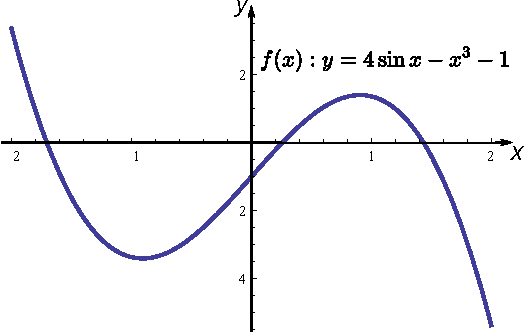
\includegraphics[scale=1]{fce_sinx.pdf}
           \captionof{figure}{Graf funkce $f(x):y=4\sin x - x^3 - 1$.}
           \label{nm:fig_ex_fce_sinx}
           \par}
        Z obrázku \ref{nm:fig_ex_fce_sinx} zjistíme, že existují tři kořeny: $x_1^*\in(-2,-1),
        x_2^*\in(-1, 0)$ a $x_3^*\in(1, 2)$.
      \end{example}
  
      Z obrázku zjistíme, že existují tři kořeny: $x_1^*\in(-2,-1),x_2^*\in(0,1),x_3^*\in(1,2)$.
      Zkusme najít kořeny v těchto intervalech pomocí numerických metod popsaných v následujících
      odstavcích
  
    \subsection{Metoda bisekce}
      Metoda známá také jako \textbf{metoda půlení intervalů}, je založena na principu
      zna\-mén\-ko\-vých změn. Předpokládejme, že funkce $f(x)$ má v koncových bodech intervalu
      $(a_0,b_0)$ opačná znaménka, tj. platí $f(a_0 )\cdot f(b_0 )<0$. Sestrojíme posloupnost
      intervalů $(a_1,b_1)\supset(a_2,b_2)\supset(a_3,b_3)\supset\cdots$, které obsahují kořen.
      Intervaly $(a_{k+1},b_{k+1}), k=0,1,\cdots$, určíme rekurzivně způsobem, který si nyní
      popíšeme.
  
      Střed intervalu $(a_k,b_k)$ je bod $x_{k+1}=\frac{1}{2}(a_k+b_k)$. Když $f(x_k)=0$, pak
      $x_{k+1}=x^*$ je kořen a dál nepokračujeme.

} %tikzset
%---------------------------------------------------------------------------------------------------
%\printbibliography[heading=subbibliography]
\addcontentsline{toc}{section}{Seznam literatury}
}
{
% DEBUG was off
%-------------------Introduction to mathematical analysis -----------------------------------------
  % !TeX spellcheck = cs_CZ
%     An overview of high school mathematics

{\tikzset{external/prefix={tikz/MAI/}}
 \tikzset{external/figure name/.add={ch01_}{}}
%---------------------------------------------------------------------------------------------------
% intro_MA.tex
%---------------------------------------------------------------------------------------------------
\chapter{Historie matematické analýzy}\label{mai:IchapI}
\minitoc


  Analýza jako nezávislý předmět byla vytvořena v 17. stol. během vědecké revoluce. Kepler, 
  Galilei, Descartes, Fermat, Huygens, Newton a Leibniz, když zmíníme jen několik důležitých jmen 
  těch, kteří přispěli k jejímu vzniku. Otázky z mechaniky, optiky a astronomie hráli roli v jejím 
  raném období, tak jako vnitřní problémy matematiky, jako výpočet obsahů, objemů a analýza 
  komplikovaných křivek. Pohyb po zakřivených drahách působením proměnných sil, které se staly 
  předmětem důkladného zájmu po studiu volně padajících těles Galilea, vedl k počátečnímu úspěchu. 
  Z velké rozmanitosti snah, které se objevily na konci 17. stol. v práci Newtona a Leibnize, se 
  zrodila nová matematická disciplína, jejíž některé poznatky jsou v těchto studijních zápiscích.
  
  Základní myšlenka použití diferenciálních rovnic k získání pohledu na globální chování proměnných kvantit z jejich (infinitezimálních) změn prokázala základní a plodné výsledky daleko za hranicemi matematiky a fyzika a formovala náš souhrnný vědecký pohled na svět, zvláště na představu o kauzalitě. Na konci 18. stol., vskutku, největší vědci došli ke shodě, že procesy v přírodě (a společnosti) jsou determinovány a podřízeny zákonům, které mohou být popsány v podobě 
  diferenciálních rovnic. Laplace, tento mistr matematické fyziky, naznačil obraz nějaké fiktivní 
  vševědoucí inteligence, užívající úplnou znalost zákonů a stavu světa v daný časový okamžik, by 
  mohla předpovídat další vývoj světa navždy a hned. Myšlenka \emph{přírodních zákonů} byla kmotrem 
  při vytvoření matematického pojmu funkce a naopak nebyla by to myšlenka nikdy tak vlivná, kdyby 
  matematická analýza nevyvíjela úspěšné metody pro výzkum funkčních závislostí. 

} % tikzset
%---------------------------------------------------------------------------------------------------
%\printbibliography[title={Seznam literatury}, heading=subbibliography]
\addcontentsline{toc}{section}{Seznam literatury}
                
%---------------------Reálná a komplexní čísla-----------------------------------------------------
  % !TeX spellcheck = cs_CZ
% Basis of Linear Algebra:
{\tikzset{external/prefix={tikz/MAI/}}
 \tikzset{external/figure name/.add={ch02_}{}}
%---------------------------------------------------------------------------------------------------
% intro_linear_algebra.tex
%---------------------------------------------------------------------------------------------------
% ==================================================================================================
% In linear algebra, a basis is a set of linearly independent vectors that, in a
% linear combination, can represent every vector in a given vector space or free
% module, or, more simply put, which define a "coordinate system".[1] In more
% general terms, a basis is a linearly independent spanning set. 
% --------------------------------------------------------------------------------------------------
\chapter{Základy lineární algebry}\label{mai:IchapII}
\minitoc
  \section{Všemocná úměra aneb lineární algebra poprvé}
    Tuto kapitolu bychom mohli opatřit podtitulem \emph{„To nejnutnější z lineární algebry“}. 
    Dovíme se v ní, co je třeba si představit pod pojmem \emph{„linearita“}, najdeme příklady 
    linearity v geometrii i v přírodovědě (fyzice, chemii, biologii) a formulujeme základní 
    poznatky týkající se řešení soustav lineárních rovnic. Do této oblasti patří i počítání s 
    vektory a maticemi — objekty, které jsou velmi vhodné k vyjádření fyzikálních veličin.
    
    \subsection{Lineární rovnice}
      Co tedy znamená slovo \textbf{linearita}? Pochází z latiny, \emph{linea recta = přímka}, 
      česky bychom řekli \emph{přímá úměrnost} nebo jen jednoduše \emph{úměra}.
      
      Nejjednodušší příklady linearity patří do oblasti geometrie — vyjádření \emph{přímek} a 
      \emph{rovin}. Jistě si ze střední školy vzpomínáme, že body těchto útvarů popisujeme jejich 
      souřadnicemi na přímce \(\mathcal{R}\), v rovině \(\mathcal{R}^2\), v prostoru 
      \(\mathcal{R}^3\). Souřadnice bodu v rovině tedy tvoří \emph{uspořádanou dvojici} reálných
      čísel, v prostoru pak \emph{uspořádanou trojici} reálných čísel. (Pozor, dvojice \([a, b]\) a 
      \([b, a]\) představují různé body.)

      %---------------------------------------------------------------
        % !TeX spellcheck = cs_CZ
% Musilova2009MA1

\begin{example}\label{mai:exam001}
  \textbf{Parametrické vyjádření přímky}\newline
  \emph{Přímka} — jednorozměrný lineární útvar v jednorozměrném prostoru \(\mathcal{R}^1\), 
  dvojrozměrném prostoru \(\mathcal{R}^2\), trojrozměrném prostoru \(\mathcal{R}^3\) (nebo i 
  n-rozměrném prostoru \(\mathcal{R}^n\)), je určena dvěma body, třeba \(A\) a \(B\), nebo
  ekvivalentně, bodem \(A\) a \emph{směrovým} vektorem \(\vec{u}\) (obr. \ref{mai:fig000}). 
  Je-li \(X\) obecným bodem na této přímce, je vektor \(\overrightarrow{AX}\) rovnoběžný, tj. 
  \emph{kolineární}, se směrovým vektorem \(\vec{u}\). (Jako směrový můžeme samozřejmě 
  použít i vektor \(\overrightarrow{AB}\).) Vektor \(\overrightarrow{AX}\) má tedy s vektorem 
  \(\vec{u}\) stejný směr, lišit se může velikostí nebo orientací. Tuto skutečnost zapíšeme 
  tak, že \(\overrightarrow{AX}\) je \emph{t}-násobkem vektorů \(\vec{u}\),
  \begin{equation*}
  \overrightarrow{AX} = t \cdot \vec{u}.
  \end{equation*}
  {\centering
    \captionsetup{type=figure}
    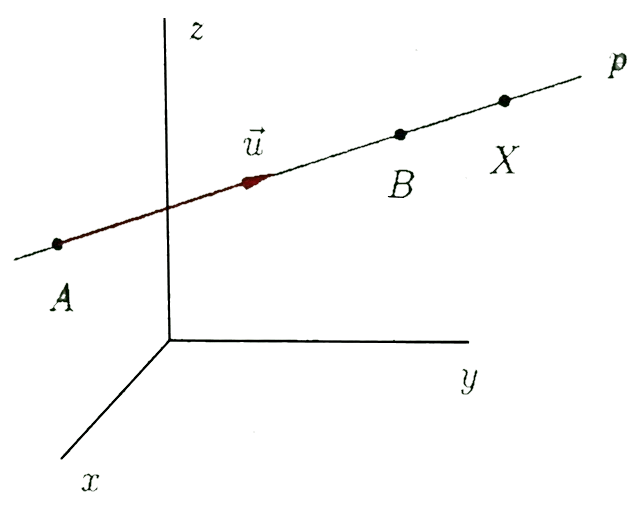
\includegraphics[width=0.5\linewidth]{mai_fig000.png}
    \captionof{figure}{Zadáni přímky. \cite[s.~1]{Musilova2009MA1}
    \label{mai:fig000}}
    \par}        
  Veličinou \(t\), takzvaným \emph{parametrem}, který může nabývat všech reálných hodnot, 
  \(t\in\mathcal{R}\), dokážeme popsat všechny vektory \(\overrightarrow{AX}\), jejichž 
  koncový bod \(X\) leží na přímce \(p\). Naopak, žádné jiné body \(X\) než ty, které leží na 
  přímce \(p\), tuto vlastnost nemají. S označením bodů \(A\), \(X\), resp. vektorů 
  \(\vec{u}\), \(\overrightarrow{AX}\) kartézskými souřadnicemi, resp. složkami
  \begin{align*}
                    A &= (x_A,y_A, z_A), \\ 
                    X &=(x,y,z),         \\
              \vec{u} &= (u_1,u_2,u_3),  \\ 
  \overrightarrow{AX} &= (x - x_A, y - y_1A, z-z_A),
  \end{align*}
  dostáváme \textbf{parametrické vyjádřeni přímky} \(p\) ve tvaru
  \begin{equation}
    p = \left\{(x,y,z)\in\mathcal{R}^3\,|\,
    \begin{matrix}
      x = x_A + tu_1,        \\
      y = y_A + tu_2,        \\
     z = z_A + tu_3,
    \end{matrix}
    \;t\in\mathcal{R}
    \right\}. \label{MAI:eq_M001}
  \end{equation}
\end{example}
\normalsize
      %---------------------------------------------------------------
      Vidíme, že kartézské souřadnice bodu na přímce se vůči souřadnicím bodu \(A\) mění přímo 
      úměrně v závislosti na hodnotě parametru \(t\), tj. závisí na jeho první mocnině. Příslušná 
      závislost se nazývá \textbf{lineární funkcí}.
      
      Obdobně zapíšeme parametrické vyjádření roviny v \(\mathcal{R}^3\):
      %---------------------------------------------------------------
      % !TeX spellcheck = cs_CZ

\begin{example}\label{mai:exam004}
  \textbf{Parametrická vyjádření roviny}:\newline
  Rovina v trojrozměrném prostoru \(\mathcal{R}^3\) je zadána třemi body \(A\), \(B\) a \(C\), 
  které nesmějí ležet v jedné přímce, popřípadě dvěma body \(A\) a \(B\) a vektorem v nerovnoběžným 
  s \(\overrightarrow{AB}\), anebo bodem \(A\) a dvěma nerovnoběžnými směrovými vektory \(\vec{u}\) 
  a \(\vec{u}\) (obr. \ref{MAI:FIG002}). Všechny tyto typy zadání jsou ekvivalentní. Lze volit 
  například \(\vec{u} = \overrightarrow{AB}\), \(\vec{v} = \overrightarrow{AC}\). Je-li \(X\) 
  libovolným bodem roviny \(\varrho\), jsou vektory \(\overrightarrow{AX}\), \(\vec{u}\) a 
  \(\vec{v}\) \textbf{lineárně závislé}. To znamená, že existují taková reálná čísla \(r\) a \(s\), 
  že vektor \(\overrightarrow{AX}\) lze zapsat jako lineární kombinaci

  {\centering
    \captionsetup{type=figure}
    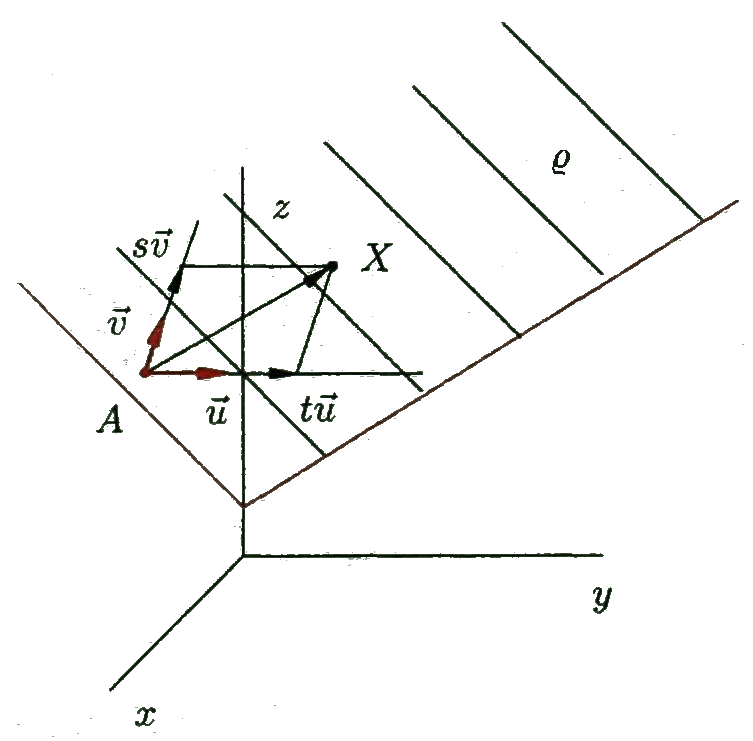
\includegraphics[width=0.5\linewidth]{Musilova_FIG002.png}
    \captionof{figure}{Zadáni roviny. \cite[s.~3]{Musilova2009MA1}}
    \label{MAI:FIG002}
    \par}  
  
\end{example}
  
      %---------------------------------------------------------------
      
    \subsection{Soustavy lineárních rovnic a jejich rychlé řešení}
      Příkladů linearity v přírodě bychom mohli nalézt bezpočet. Vraťme se však k matematice a k 
      problematice uvedené v názvu tohoto odstavce, k soustavám lineárních rovnic. Začněme 
      jednoduchou slovní úlohou ze základní školy:

      %---------------------------------------------------------------
      % !TeX spellcheck = cs_CZ

\begin{example}\label{mai:exam005}
  \textbf{Příklad s ježibabou:}\newline
  Jeníček a Mařenka kradli ježibabě perník. Dohromady snědli 11 perníkových srdíček. Jeníček jich 
  přitom zkonzumoval o 3 více než Mařenka. Otázka je tradiční — kolik srdíček snědl každý z nich?
  Označíme-li \(M\) počet kousků, které snědla Mařenka a \(J\) počet srdíček, na nichž si pochutnal 
  Jenda, můžeme informace zadané v úloze zapsat takto:
    \begin{equation*}
      M + J = 11 \qquad J = M + 3.
    \end{equation*}
  Řešení není problémem, snadno vidíme, že \(M = 4\) a \(J = 7\).
\end{example}
      %---------------------------------------------------------------
      
      O samotné řešení této jednoduché úlohy v tuto chvíli nejde. Pojmenujme si však vztahy, které 
      jsme pro neznámé hodnoty \(M\) a \(J\) ze zadání úlohy dostali. Neznámé vystupují v 
      rovnicích v první mocnině, tedy \emph{lineárně}. Máme \emph{soustavu dvou rovnic} o dvou 
      neznámých \(M\) a \(J\). Úvahu snadno zobecníme: Předpokládejme, že máme neznámé veličiny
      \begin{equation*}
        (x_1, x_2, \ldots, x_n)
      \end{equation*}
      a máme o nich \(m\) informací, které lze zapsat ve tvaru lineárních rovnic (neznámé budou v 
      těchto rovnicích vystupovat v první mocnině),
      \begin{align}
        a_{11}x_1 + a_{12}x_2 + \ldots + a_{1n}x_n &= b_1,     \nonumber           \\
        a_{21}x_1 + a_{22}x_2 + \ldots + a_{2n}x_n &= b_2,     \label{mai:eq002}   \\
        .......................................... &= \ldots   \nonumber           \\
        a_{m1}x_1 + a_{m2}x_2 + \ldots + a_{mn}x_n &= b_m,     \nonumber
      \end{align}
      Soustavu (\ref{mai:eq002}) nazýváme soustavou \(m\) lineárních rovnic o \(n\) neznámých. 
      Označme ji jako \(S\) a pod tímto označením se k ní budeme vracet. Soubory reálných čísel 
      \((a_{ij})\) a \((b_i)\), kde \(1 < i < m\), \(1 \leq j < n\), jsou zadány. Lze je uspořádat 
      do takzvaných \textbf{matic}
      \begin{equation}\label{mai:eq003}
        A =
          \begin{pmatrix}
            a_{11} & a_{12} & \ldots & a_{1n} \\
            a_{21} & a_{22} & \ldots & a_{2n} \\
            \ldots & \ldots & \ldots & \ldots \\
            a_{m1} & a_{m2} & \ldots & a_{mn}          
          \end{pmatrix},
          \overline{B} =
          \begin{pmatrix}
            b_1     \\
            b_2     \\
            \ldots  \\
            b_m 
          \end{pmatrix}
      \end{equation}
      
      Matice \(A\) je typu \(m/n\), má \(m\) řádků a \(n\) sloupců, \(i\) je řádkový index a \(j\) 
      je sloupcový index. Matice \(\overline{B}\) je typu \(m/1\) (\(m\) řádků a jeden sloupec), 
      hovoříme také o sloupcové matici. Soustavu \(S\) můžeme zapsat zkráceně pomocí maticového 
      násobení (podrobněji viz později odstavec \ref{MAI:sec_matice}):
      \begin{equation*}
        A \cdot X = \overline{B}, \qquad \text{nebo}
      \end{equation*}  
      \begin{equation}\label{mai:eq004}
          \begin{pmatrix}
            a_{11} & a_{12} & \ldots & a_{1n} \\
            a_{21} & a_{22} & \ldots & a_{2n} \\
            \ldots & \ldots & \ldots & \ldots \\
            a_{m1} & a_{m2} & \ldots & a_{mn}
          \end{pmatrix}
          \cdot
          \begin{pmatrix}
            x_1     \\
            x_2     \\
            \ldots  \\
            x_m 
         \end{pmatrix}
          =
         \begin{pmatrix}
              b_1     \\
              b_2     \\
              \ldots  \\
              b_m 
            \end{pmatrix}
      \end{equation}
      V tuto chvíli vysvětlíme podstatu maticového násobení jen technicky: Násobit mezi sebou 
      můžeme matici \(A = (a_{ij})\) typu \(m/n\) (levý činitel) a matici \(C = (c_{jk})\) typu 
      \(n/p\) (pravý činitel, činitele nelze zaměňovat). Výsledkem je matice \(D = (d_{ik})\) typu 
      \(m/p\), jejíž prvky se počítají podle předpisu
      \begin{equation}\label{mai:eq005}
        d_{ik} = \sum_{j=1}^{n} a_{ij}\cdot c_{jk}.
      \end{equation}
      
      Z tohoto obecného předpisu vidíme, že levé strany soustavy \(S\) lze interpretovat ve tvaru 
      součinu matice \(A\) typu \(m/n\) s maticí neznámých typu \((n/1)\), výsledkem je matice 
      pravých stran \(\overline{B}\), která je typu \(m/1\). Matice \(A\) se nazývá \textbf{maticí 
      soustavy}. Matice, která vznikne jejím \emph{rozšířením} o sloupec pravých stran, tj.
      \begin{equation}\label{mai:eq006}
        B = (A|\overline{B}) =
        \left(
          \begin{array}{cccc|c}
            a_{11} & a_{12} & \ldots & a_{1n} & b_1    \\
            a_{21} & a_{22} & \ldots & a_{2n} & b_2    \\
            \ldots & \ldots & \ldots & \ldots & \ldots \\
            a_{m1} & a_{m2} & \ldots & a_{mn} & b_m
          \end{array}
        \right)
      \end{equation}
      je pak \textbf{rozšířenou maticí soustavy}. Je-li sloupec pravých stran soustavy tvořen 
      samými nulami, nazývá se soustava \textbf{homogenní}, v opačném případě \textbf{nehomogenní}. 
      Řešením soustavy \(S\) nazýváme každou \(n\)-tici \((x_i, x_2,\ldots, x_n)\), která soustavu 
      \(S\) splňuje. Cílem je najít všechna řešení soustavy \(S\). Abychom řešení nalezli, musíme 
      soustavu upravovat, zjednodušovat. Prováděné úpravy mají vést k jednodušší, avšak 
      ekvivalentní soustavě rovnic, tj. takové, která má naprosto stejný soubor všech řešení jako 
      soustava původní. Takové úpravy nazýváme \textbf{ekvivalentními}. Dvě základní, pomocí nichž 
      lze uskutečnit všechny ostatní, jsou
      \begin{itemize}\addtolength{\itemsep}{-0.5\baselineskip}
        \item vynásobení libovolné, například \(i\)-té, rovnice libovolným \emph{nenulovým} číslem,
        \item přičtení \(i\)-té rovnice vynásobené libovolným číslem k \(l\)-té rovnici.
      \end{itemize}      
      V soustavě lze samozřejmě také měnit pořadí rovnic. Tato úprava je rovněž ekvivalentní. 
      Nevypisujeme ji však zvlášť proto, že ji lze realizovat pomocí vhodně zvolené posloupnosti 
      základních dvou úprav.
      
      Abychom nemuseli soustavu stále opisovat i s neznámými, provádíme obvykle ekvivalentní 
      úpravy jen s maticí \(B = (A|\overline{B})\) (každý řádek této matice představuje jednu 
      rovnici soustavy \(S\)). Může se stát, že soustava má právě \emph{jedno řešení}, jako tomu 
      bylo v  úloze o Mařence a Jeníčkovi. Také nemusí mít \emph{řešení žádné}, jako například 
      soustava \(x + y = 0\), \(x + y = l\) (součet dvou čísel nemůže nabývat současně dvou různých 
      hodnot). A třeba má také řešení \emph{nekonečně mnoho} (řešením soustavy jedné rovnice o dvou 
      neznámých \(x + y = 1\) jsou všechny dvojice tvaru \((x, 1 — x)\), kde \(x\) je libovolné). A 
      může mít soustava \(S\) třeba právě dvě řešení? Prostřednictvím následujícího příkladu 
      ukážeme metodu, která vede velmi rychle k nalezení všech řešení a umožňuje také vyslovit 
      obecné závěry o jejich vlastnostech a počtu. Jedná se o \textbf{Gaussovu eliminační metodu}.
      
 
%--------------------------------------------------------------------------------------------------
  \section{Matice}\label{MAI:sec_matice}
    \begin{definition}\label{def_matice}
      Nechť \(m, n\) jsou přirozená čísla. Jestliže každé uspořádané dvojici \(m,n\). Jestliže každé
      uspořádané dvojici \((m,n)\in \{1,2,\ldots,m\}\times \{1,2,\ldots,m\) přiřadíme prvek
      \(a_{i,j}\in\mathcal{R}\) obdržíme reálnou \href{http://cs.wikipedia.org/wiki/Matice}{matici} 
      typu \(m,n\) nad \(\mathcal{R}\). Čísla jsou indexy, \(i\) je řádkový a \(j\) je sloupcový 
      index.
      
      Matici zapisujeme jako
      \begin{equation}\label{matice_zapis}
        A = \left(a_{ij}\right) =\left(
          \begin{array}{ccc}
            a_{11} & \ldots & a_{1n} \\
            \vdots & \ddots & \vdots \\
            a_{m1} & \ldots & a_{nn}
          \end{array}
        \right)
      \end{equation}
      která má právě \(mn\) prvků \((a_{ij})\) uspořádaných do \(m\) řádků a \(n\) sloupců. Stručně 
      píšeme \(A = (a_{ij})\)
    \end{definition}
  
    \begin{example}
      Matice \(\begin{pmatrix}1&2&3&4\\4&3&2&1\\-1&-1&-1&-1\\-2&-1&0&1\end{pmatrix}\) je čtvercová 
      matice velikosti \(4\times4\). Prvek matice \(a_{23}\) je \(2\).
    \end{example}  
    
    \subsection{Maticová algebra}
      \begin{definition} 
        Součinem matice \(A \in \mathcal{R}_{mn}\) a matice \(B \in \mathcal{R}_{np}\), v uvedeném
        pořadí, je matice \(C \in \mathcal{R}_{mp}\) pro kterou platí:
        \begin{align*}
               C &= AB; \quad C = (cij); \\
               \shortintertext{kde}
          c_{ij} &= \sum_n^{k=1}{a_{ik}b_{kj}};\quad
                     i = 1,\ldots,m; \, j = 1,\ldots,p.
        \end{align*} 
      \end{definition}
      Součin matic \(A\) a \(B\) je definován právě tehdy, když počet sloupců matice \(A\) je roven 
      počtu řádků matice \(B\). Obrázek \ref{LA:fig_LA001a} demonstruje jakým způsobem se 
      dostane prvek, který je ve výsledné matici třeba ve druhém řádku a druhém sloupci, násobením 
      druhého řádku levé matice s druhým sloupcem pravé ze zadaných matic. Stejným způsobem získáme 
      hodnotu prvku \(c_{ij}\) (viz \ref{LA:fig_LA001b}).
%      %----------------------------------
      \begin{figure}[ht!]
        \centering  
        \begin{tabular}{@{}c}
          \subfloat[1. krok]{\label{LA:fig_LA001a}
            %\documentclass[11pt]{standalone}
%  \usepackage{helvet}                        % font
%  \usepackage{xltxtra}                       % fontspec package
%  \usepackage{tikz}  
%  \usetikzlibrary{matrix, arrows}
%  \usepackage{circuitikz}

%\begin{document}

\begin{tikzpicture}

\newcommand{\unit}{0.9cm}
\tikzset{
          node  style    sp/.style={draw,circle,minimum size=\unit},
          node  style    ge/.style={circle,minimum size=\unit}, 
          arrow style   mul/.style={draw,sloped,midway,fill=white}, 
          arrow style  plus/.style={midway,sloped,fill=white},
          yl/.style={},
      }

	\matrix (A) [matrix of math nodes, row sep=-0.5em, column sep=-0.5em, 
               text height=1.5ex, text depth=0.25ex,
			   nodes={node style ge}, left delimiter={(}, right delimiter={)}] at (0,0) {
    a_{11}                          & a_{12}                          & \ldots     & 
    a_{1p}                         \\
    | [node style sp] | {a_{21}}    & | [node style sp] | {a_{22}}    & \ldots     & | [node style 
    sp] | {a_{2p}}   \\
    \vdots                          & \vdots                          & \ddots     & 
    \vdots                         \\
    a_{n1}                          & a_{n2}                          & \ldots     & 
    a_{np}                         \\
  };
    
  \matrix (B) [matrix of math nodes, row sep=-0.5em, column sep=-0.5em, 
               text height=1.5ex, text depth=0.25ex,
			   nodes={node style ge}, left delimiter={(}, right delimiter={)}] at (4.5*\unit,4.5*\unit) {
    b_{11}                          & | [node style sp] | {b_{12}}    & \ldots     & 
    b_{1q}                         \\
    b_{21}                          & | [node style sp] | {b_{22}}    & \ldots     & 
    b_{2q}                         \\
    \vdots                          & \vdots                          & \ddots     & 
    \vdots                         \\
    b_{p1}                          & | [node style sp] | {b_{p2}}    & \ldots     & 
    b_{pq}                         \\
  };
  
  % matrice result
  \matrix (C) [matrix of math nodes, row sep=-0.5em, column sep=-0.5em, 
               text height=1.5ex, text depth=0.25ex,
               nodes={node style ge}, left delimiter={(}, right delimiter={)}] at (4.5*\unit,0) {
    c_{11}                          & c_{12}                            & \ldots     & 
    c_{1q}                       \\
    c_{21}                          & | [node style sp,red] | {c_{22}}  & \ldots     & 
    c_{2q}                       \\
    \vdots                          & \vdots                            & \ddots     & 
    \vdots                       \\
    c_{n1}                          & c_{n2}                            & \ldots     & 
    c_{nq}                       \\
  };

  \draw[blue] (A-2-1.north) -- (C-2-2.north);
  \draw[blue] (A-2-1.south) -- (C-2-2.south);
  \draw[blue] (B-1-2.west)  -- (C-2-2.west);
  \draw[blue] (B-1-2.east)  -- (C-2-2.east);
  \draw[angle 60-angle 60,red](A-2-1) to[in=180,out=90] node[arrow style mul] (x) 
    {\tiny\(a_{21}\times b_{12}\)} (B-1-2);
  \draw[angle 60-angle 60,red](A-2-2) to[in=180,out=90] node[arrow style mul] (y) 
    {\tiny\(a_{22}\times b_{22}\)} (B-2-2);
  \draw[angle 60-angle 60,red](A-2-4) to[in=180,out=90] node[arrow style mul] (z) 
    {\tiny\(a_{2p}\times b_{p2}\)} (B-4-2);
  \draw[red,-angle 60] 
    (x) to node[arrow style plus] {$+$} (y)%
        to node[arrow style plus] {$+\raisebox{.5ex}{\ldots}+$} (z)%
        to (C-2-2.north west);   
  \node [draw, below=5pt] at (A.south) 
    { \tiny\(A\) : \textcolor{red}{\(n\) řádků} \(p\) sloupků};
  \node [draw, above=5pt] at (B.north) 
    { \tiny\(B\) : \(p\) řádků \textcolor{red}{\(q\) sloupků}}; 
  \node [draw, below=5pt] at (C.south) 
    {\tiny\(C=A\times B\) : \textcolor{red}{\(n\) řádků}  \textcolor{red}{\(q\) sloupků}}; 
\end{tikzpicture}
%\end{document}}              \\
          \subfloat[2. krok]{\label{LA:fig_LA001b}
            %\documentclass[11pt]{standalone}
%  \usepackage{helvet}                        % font
%  \usepackage{xltxtra}                       % fontspec package
%  \usepackage{tikz}  
%  \usetikzlibrary{matrix, arrows,decorations}
%  \usepackage{circuitikz}





%\begin{document}
\begin{tikzpicture}

\newcommand{\unit}{0.9 cm}
  \tikzset{
          node  style    sp/.style={draw,circle,minimum size=\unit},
          node  style    ge/.style={circle,minimum size=\unit}, 
          arrow style   mul/.style={draw,sloped,midway,fill=white}, 
          arrow style  plus/.style={midway,sloped,fill=white},
          yl/.style={},
      }

  % defintion of matrices
  \matrix (A) [matrix of math nodes, row sep=-0.9em, column sep=-0.9em, 
               text height=1.5ex, text depth=0.25ex,
			   nodes={node style ge}, left delimiter={(}, right delimiter={)}] at (0,0) {
    a_{11}                       & \ldots & a_{1k}                        & \ldots & 
    a_{1p}                       \\
    \vdots                       & \ddots & \vdots                        & \vdots & 
    \vdots                       \\
    | [node style sp] | {a_{i1}} & \ldots & | [node style sp] | {a_{ik}}  & \ldots & | [node style 
    sp] | {a_{ip}} \\
    \vdots                       & \vdots & \vdots                        & \ddots & 
    \vdots                       \\
    a_{n1}                       & \ldots & a_{nk}                        & \ldots & 
    a_{np}                       \\
  };

  \matrix (B) [matrix of math nodes, row sep=-0.9em, column sep=-0.9em, 
               text height=1.5ex, text depth=0.25ex,
               nodes={node style ge}, 
               left delimiter={(}, right delimiter={)}] at (4.7*\unit,4.0*\unit) {
    b_{11} & \ldots & | [node style sp] | {b_{1j}} & \ldots & b_{1q}  \\
    \vdots & \ddots & \vdots                       & \vdots & \vdots  \\
    b_{k1} & \ldots & | [node style sp] | {b_{kj}} & \ldots & b_{kq}  \\
    \vdots & \vdots & \vdots                       & \ddots & \vdots  \\
    b_{p1} & \ldots & | [node style sp] | {b_{pj}} & \ldots & b_{pq}  \\
  };

  % matrice resultat
  \matrix (C) [matrix of math nodes, row sep=-0.9em, column sep=-0.9em, 
               text height=1.5ex, text depth=0.25ex,
               nodes={node style ge}, left delimiter={(}, right delimiter={)}] at (4.7*\unit,0) {
    c_{11} & \ldots & c_{1j}                           & \ldots & c_{1q} \\
    \vdots & \ddots & \vdots                           & \vdots & \vdots \\
    c_{i1} & \ldots & | [node style sp,red] | {c_{ij}} & \ldots & c_{iq} \\
    \vdots & \vdots & \vdots                           & \ddots & \vdots \\
    c_{n1} & \ldots & c_{nk}                           & \ldots & c_{nq} \\
  };

  % arrows
  \draw[blue] (A-3-1.north) -- (C-3-3.north);
  \draw[blue] (A-3-1.south) -- (C-3-3.south);
  \draw[blue] (B-1-3.west)  -- (C-3-3.west);
  \draw[blue] (B-1-3.east)  -- (C-3-3.east);
  \draw[<->,red](A-3-1) to[in=180,out=90] node[arrow style mul] (x)
    {\tiny\(a_{i1}\times b_{1j}\)} (B-1-3);
  \draw[<->,red](A-3-3) to[in=180,out=90] node[arrow style mul] (y) 
    {\tiny\(a_{ik}\times b_{kj}\)} (B-3-3);
  \draw[<->,red](A-3-5) to[in=180,out=90] node[arrow style mul] (z) 
    {\tiny\(a_{ip}\times b_{pj}\)} (B-5-3);
  \draw[red,->] 
    (x) to node[arrow style plus] {$+\raisebox{.5ex}{\ldots}+$} (y)%
        to node[arrow style plus] {$+\raisebox{.5ex}{\ldots}+$} (z);
      % to (C-3-3.north west);
  \draw[->,red] (z) -- (C-3-3.north west);
  \node [draw, below=5pt] at (A.south) 
    { \tiny\(A\) : \textcolor{red}{\(n\) řádků} \(p\) sloupků};
  \node [draw, above=5pt] at (B.north) 
    { \tiny\(B\) : \(p\) řádků \textcolor{red}{\(q\) sloupků}}; 
  \node [draw, below=5pt] at (C.south) 
    {\tiny\(C=A\times B\) : \textcolor{red}{\(n\) řádků}  \textcolor{red}{\(q\) sloupků}}; 
\end{tikzpicture}
%\end{document}}
        \end{tabular}
        \caption{Postup při maticovém násobení}
      \end{figure}

%--------------------------------------------------------------------------------------------------
    \subsection{Označení prvků matice}
      Prvky matice jsou označeny indexy udávajícími \textbf{řádek} a \textbf{sloupec}, v nichž se 
      prvek nalézá. Prvek v \(i\)-tém řádku a \(j\)-tém sloupci matice \(A\) se obvykle značí 
      \(a_{ij}\). Potom \(i\)-tý řádek matice  obsahuje vodorovnou \(n\)-tici prvků \(a_{i1}, 
      a_{i2}, \ldots,a_{in} \), kde \(i=  1,2,\ldots,m\) a \(j\)-tý sloupec matice obsahuje svislou 
      matici čísel \(a_{1j},a_{2j},\ldots,a_{mj}\), kde \(j = 1,2,\ldots,n\).
  
      V tabulce \ref{LA:tab_basic_matrix} jsou uvedeny nejčastější typy matic, které se v algebře 
      často vyskytují. Jsou to například matice řádkové, sloupcové, diagonální\footnote{Prvky 
      \(a_{ii}\) kde \(i=1,2,\ldots,\min(m,n)\) tvoří hlavní diagonálu. Matice \(\mathbf{D}\) je 
      typu \(m,m\), obecně může mít diagonální matice buď ještě další sloupce, v nichž budou samé 
      nuly, anebo další řádky, v nichž budou opět samé nuly.}, jednotkové\footnote{Jestliže \(m = 
      n\), pak mluvíme o čtvercové matici řádu \(m\).}, nulové, transponované a symetrické.
  
      \begin{table}[!ht]
          \centering
          \renewcommand{\arraystretch}{1.8}   % for the vertical padding
            \begin{tabular}{|l||c@{}|}              
              \hline 
              \textbf{Matice}                    & \textbf{Zápis} \\ \hline\hline
              \ttfamily řádková   \(\mathbf{A}\) &  \(a_1,a_2,\ldots,a_n \)\\
              \ttfamily sloupcová \(\mathbf{B}\) & 
                \(\begin{pmatrix}
                  a_1     \\
                  a_2     \\
                  \vdots  \\
                  a_n
                \end{pmatrix}\)                       \\
              \ttfamily diagonální \(\mathbf{C}\) & 
                \(\begin{pmatrix}
                   a_{11} &    0   & \ldots &   0     \\
                      0   & a_{22} & \ldots &   0     \\
                   \vdots & \vdots & \ddots & \vdots  \\
                      0   &   0    & \ldots & a_{mm}
                \end{pmatrix}\)                       \\
              \ttfamily jednotková \(\mathbf{I}\) &
                \(\begin{pmatrix}
                     1    &    0   & \ldots &   0    \\
                     0    &    1   & \ldots &   0    \\
                   \vdots & \vdots & \ddots & \vdots \\
                      0   &   0    & \ldots & 1
                \end{pmatrix}\)                      \\
              \ttfamily nulová \(\mathbf{0}\) & \((a_{ij}),\quad a_{ij} = 0\,\forall\,i, j\) \\
              \ttfamily transponovaná \(\mathbf{D^T}\) &
                \(\begin{pmatrix}
                  a_{11} & a_{21} & \ldots &  a_{m1}\\
                  a_{12} & a_{22} & \ldots &  a_{m2}\\
                  \vdots & \vdots & \ddots & \vdots \\
                  a_{1n} & a_{2n} & \ldots & a_{mn}
                \end{pmatrix}\)    \\
              \ttfamily symetrická \(\mathbf{S}\) 
              & \((a_{ij}),\quad a_{ij}= a_{ji}\,\forall\,i,j\) \\ \hline
            \end{tabular}
          \caption{Speciální typy matic}\label{LA:tab_basic_matrix}
      \end{table}
    
    
      Matice téhož typu \((m,n)\) nad \(\Re\) budeme značit \(\Re_{m,n}\).
      
      \begin{definition}\label{rovnost_matic}
       (Rovnost matic):  Matice \(\mathbf{A} = \left(a_{ij}\right)\) je rovna matici \(\mathbf{B}=
       \left(b_{kl}\right)\), jsou-li matice stejného typu a stejnolehlé prvky se sobě
       \textbf{rovnají}, tj. \(\mathbf{A} \in \Re_{m,n}, \mathbf{B}\in\Re_{m,n}, a_{ij} = b_{ij}, 
       \forall i\in\lbrace1,2,\ldots,m\rbrace, \forall j\in\lbrace1,2,\ldots,n\rbrace\).
      \end{definition}
      
  %===============================Kapitola: Vektory================================================
  \section{Počítání s vektory}
    \textbf{Vektory} budeme nazývat matice typu \(1/n\) a značit je
    \begin{equation*}
      \vec{u} = (u_1, u_2, \ldots, u_n).
    \end{equation*}
    Takže počítat s nimi již umíme! (V zápisu složek vektoru je vynechán řádkový index. V případě 
    matice s jedním řádkem, takzvané \emph{řádkové matice}, je totiž zbytečný.) Číslům \(u_1\) až 
    \(u_n\) budeme pro tuto chvíli říkat \emph{složky vektoru} \(\vec{u}\). Za chvíli tento pojem 
    ještě upřesníme. Celou řadu pojmů, s nimiž jsme se seznámili při počítání s maticemi, můžeme 
    pro vektory přímo použít. Namísto značení \(\mathcal{M} (1/n)\) budeme pro prostor vektorů 
    používat symbol \((\mathcal{R}^n)\) nebo \(\mathcal{C}^n\) (obvyklý symbol pro množinu 
    uspořádaných \(n\)-tic reálných nebo komplexních čísel).
    
    \subsection{Součiny vektorů}
      Kromě základních operací s vektory, tj. sčítání vektorů a násobení vektoru skalárem, se 
      často používají další operace, které obohacují \emph{strukturu vektorového prostoru}. 
      Zůstaneme u vektorů v trojrozměrném prostoru \(\mathcal{R}^3\) a definujeme si skalární, 
      vektorový a smíšený součin vektorů. Skalární součin vektorů definujeme prostřednictvím 
      geometrické definice jako zobrazení, které uspořádané dvojici vektorů (volných vektorů nebo 
      jejich libovolných umístění) přiřazuje reálný číslo podle předpisu
      
  %===============================Kapitola: Determinanty===========================================
  \section{Determinanty}
    Abychom mohli nadefinovat determinant, budeme muset vědět, jak vypočítat permutaci entice, 
    respektive znaménko permutace.
    \subsection{Permutace}
      \begin{definition}\label{permutace}
        Nechť \(\mathbf{M}\) je libovolná konečná množina. Permutací množiny \(M\) nazýváme 
        zobrazení \(\pi\) množiny \(\mathbf{M}\) na sebe.
      \end{definition}
      
      \begin{example}%(Damlová  Nagy, 1985, str. 34)
        Permutace \(\pi\) množiny \(\mathbf{M}= \lbrace a,b,c,d\rbrace\) je např. zobrazení 
        \(\pi\), definované předpisem:
        \begin{equation}\label{permutace_zadani}
          \pi\left(a\right) = c, \,
          \pi\left(b\right) = d, \,
          \pi\left(c\right) = b, \,
          \pi\left(d\right) = a,
        \end{equation}
        Místo tohoto zápisu se však používá přehlednější zápis ve tvaru matice typu \((2,4)\):
        \begin{equation}\label{LA:eq_perm_exam}
            \begin{pmatrix}
            a & b & c & d \\
            c & d & b & a
            \end{pmatrix}
        \end{equation}
        kde v prvním řádku jsou vypsány všechny prvky množiny \(\mathbf{M}\) (v libovolném pořadí) 
        a ve druhém řádku je pod každým prvkem zapsán jeho obraz v permutaci. Tutéž permutaci však 
        můžeme zapsat ve tvaru matice několika různými způsoby. Například mohou být zapsány takto:
        \begin{equation}
          \begin{array}{cc}
            \begin{pmatrix}
              b & a & c & d \\
              d & c & b & a
            \end{pmatrix},         & 
            \begin{pmatrix}
              d & c & b & a \\
              a & b & d & c
            \end{pmatrix}          \\
            \begin{pmatrix}
              d & c & a & b \\
              a & b & c & d
            \end{pmatrix},         &
            \text{apod.}
          \end{array}
        \end{equation}
      \end{example}

      Zřejmě všechny čtyři uvedené zápisy permutace rov. \ref{LA:eq_perm_exam} ve tvaru matice se 
      liší navzájem pouze pořadím sloupců. Aby bylo možné zapsat každou permutaci množiny 
      \(\mathbf{M}\) ve tvaru rov. \ref{LA:eq_perm_exam} jediným způsobem, je nutné zvolit pevné 
      pořadí prvků množiny \(\mathbf{M}\)  a v zápisu permutace uvádět prvky matice \(\mathbf{M}\)  
      v prvním řádku v tomto pořadí. Avšak známe-li toto pořadí prvků množiny \(\mathbf{M}\), je 
      pak  obvykle zbytečné jej v zápisu permutace uvádět, ale stačí uvést pouze pořadí obrazů, tj. 
      druhý řádek. Zvolíme-li např. v naší množině \(\mathbf{M}\) pevné pořadí prvků \(\lbrace 
      a,b,c,d\rbrace\), pak permutaci rov. \ref{permutace_zadani} zapíšeme jako uspořádanou 
      čtveřici \(\lbrace c,d,b,a\rbrace\).
  
      \begin{definition}\label{def_permutace_ntice}
        Když vytváříme uspořádanou \(n\)-tici navzájem různých prvků \(n\)-prv\-ko\-vé množiny 
        \(\mathbf{M}\), přiřazujeme každému prvku množiny \(\mathbf{M}\) právě jedno přirozené 
        číslo, index příslušného prvku, z množiny prvních \(n\) přirozených čísel.
        \begin{equation}\label{permutace_ntice}
          \pi = \lbrace 1, 2, 3, \ldots, n\rbrace
        \end{equation}
      \end{definition}
  
      Proto každé permutaci uspořádané \(n\)-tice prvků množiny \(\mathbf{M}\) odpovídá jednoznačně 
      permutace příslušných indexů tj. permutace množiny \ref{permutace_ntice} z definice 
      \ref{def_permutace_ntice}. Stačí se tedy omezit při vyšetřování permutací n-prvkové množin 
      na vyšetřování permutací množiny \ref{permutace_ntice}. Permutace \(\pi\) množiny 
      \ref{permutace_ntice} budeme zapisovat jako uspořádané \(n\)-tice \(\left(\pi(1), \pi(2) 
      ,\ldots, \pi(n)\right)\), kde \(\pi(i)\) je číslo z množiny \ref{permutace_ntice}, které 
      permutace \(\pi\) přiřazuje číslu \(i\).

      \begin{example}\label{ex_celk_pocet_permutaci}
        \textbf{Spočítejme celkový počet permutací množiny}. V každé uspořádané \(n\)-tici může být 
        na prvním místě kterákoli z \(n\) cifer, na druhém místě kterákoli ze zbývajících \(n-1\) 
        cifer (kromě té, která je na prvním místě), na  třetím místě každá ze zbývajících \(n-2\) 
        cifer atd. Je tedy celkový počet všech permutací \(n\)-prvkové množiny \(n(n-1)(n-2)\cdot 
        \ldots \cdot2\cdot1\). Toto číslo se zapisuje pomocí symbolu \(n!\) (čti 
        \textbf{n-faktoriál}).
      \end{example}
      
      \begin{definition}\label{def_inv_perm}\textbf{Inverze v permutaci}:
        Inverzí v permutaci \(\left(i_1,i_2,…,i_n \right)\) rozumíme každý výskyt takové dvojice 
        čísel, že větší stojí před menším, tj. vlevo od něj.
      \end{definition}  
   
  %=========================== Kapitola: Vlastní čísla a vlastní vektory ==========================
  \section{Vlastní čísla a vlastní vektory}
    \subsection{Motivace} 
      \textbf{Poznámka}: Je-li \(\mathcal{A} : \mathcal{V} \rightarrow \mathcal{V}\) lineární 
      zobrazení z prostoru \(\mathcal{V}\) do prostoru \(\mathcal{V}\) (nikdy se takové zobrazení 
      nazývá lineárním operátorem), pak je přirozeným požadavkem najít takovou bázi prostoru 
      \(\mathcal{V}\), že je matice zobrazení $\mathbf{A}$ v této bázi co nejjednodušší, např. má 
      následující strukturu
      \begin{equation*}
         \mathbf{A}=
           \left(\begin{array}{ccccc}
             \boxed{A_1}       &             &       &       & 0   \\
                 & \boxed{A_2} &             &       &             \\
                 &             & \boxed{A_3} &       &             \\
                 &             &             &\ddots &             \\
              0  &             &             &       & \boxed{A_k}
            \end{array}
           \right),
     \end{equation*}
     kde \(A_k\) jsou čtvercové matice malého řádu (nejlépe \(1\) nebo \(2\)) a ostatní prvky 
     matice jsou nulové. Problém najít bázi, aby v ní matice zobrazení měla diagonální tvar (kde 
     \(A_k\) jsou skaláry), vede k pojmu vlastní číslo a vlastní vektor matice.

      \begin{definition} 
        Nechť \(\mathbf{A}\in \mathcal{C}^{n,n}\) (matice je čtvercová řádu \(n\)).
        \begin{equation}
          \mathbf{A} = (a_{ij}) =
            \begin{pmatrix}
              a_{11} & a_{12} & \ldots & a_{1n} \\
              a_{21} & a_{22} & \ldots & a_{2n} \\
              \vdots & \vdots & \ddots & \vdots \\
              a_{n1} & a_{n2} & \ldots & a_{nn}
            \end{pmatrix}
        \end{equation}

        Jestliže platí
        \begin{equation}\label{eq:vl_number}
          \mathbf{Au} = \lambda\mathbf{u}
        \end{equation}
        pro jisté komplexní číslo \(\lambda\in\mathcal{C}\)  a jistý nenulový vektor 
        \(x\in\mathcal{C}^n, \mathbf{u}\neq\Theta\), potom číslo \(\lambda\) nazýváme 
        \textbf{vlastním číslem} matice \(\mathbf{A}\) a vektor \(\mathbf{u}\) \textbf{vlastním 
        vektorem} příslušným k tomuto vlastnímu číslu. Množinu všech vlastních čísel nazýváme 
        \textbf{spektrem matice} \(\mathbf{A}\). Pokud rov. \ref{eq:vl_number} rozepíšeme, dostaneme
        \begin{equation}
          \begin{pmatrix}
            a_{11} & a_{12} & \ldots & a_{1n} \\
            a_{21} & a_{22} & \ldots & a_{2n} \\
            \vdots & \vdots & \ddots & \vdots \\
            a_{n1} & a_{n2} & \ldots & a_{nn}
          \end{pmatrix}   \cdot
          \begin{pmatrix}
            u_{1} \\  u_{2} \\ \vdots \\  u_{n} \\
          \end{pmatrix}    =\lambda\cdot
          \begin{pmatrix}
            u_{1} \\ u_{2} \\ \vdots \\ u_{n} \\
          \end{pmatrix}
        \end{equation}
        můžeme ji rovněž psát ve tvaru
        \begin{equation*}
            \begin{pmatrix}
            \setlength{\arraycolsep}{3pt}
              a_{11} -\lambda & a_{12}           & \ldots & a_{1n} \\
              a_{21}          & a_{22} -\lambda  & \ldots & a_{2n} \\
              \vdots          & \vdots           & \ddots & \vdots \\
              a_{n1}          & a_{n2}           & \ldots & a_{nn}-\lambda
            \end{pmatrix} \cdot
          \begin{pmatrix}
            u_{1} \\ u_{2} \\ \vdots \\ u_{n} \\
          \end{pmatrix}  =
          \begin{pmatrix}
              0 \\ 0 \\ \vdots \\ 0 \\
            \end{pmatrix}
        \end{equation*}
      \end{definition}

       Tato soustava rov. je \textbf{homogenní} a stručně ji můžeme zapsat
      \begin{equation}\label{vv_hom_zapis}
        \left(\mathbf{A} - \lambda\mathbf{I}\right) = \mathbf{0}
      \end{equation}
      Homogenní soustava má \emph{netriviální řešení}, právě když je determinant matice soustavy 
      roven  nule, tj. v případě soustavy rov. rov. \ref{vv_hom_zapis} platí
      \begin{equation}\label{vv_hom_reseni}
        |\mathbf{A} - \lambda\mathbf{I}| = \mathbf{0}
      \end{equation}
      Determinant \(A(\lambda)=|\mathbf{A} - \lambda \mathbf{I}|\) nazýváme 
      \textbf{charakteristický polynom} matice \(\mathbf{A}\) - jedná se o polynom stupně \(n\) v 
      proměnné \(\lambda\), který má v oboru komplexních čísel \(n\) kořenů. Rovnici 
      \(A(\lambda)=0\) nazýváme \textbf{charakteristická rovnice matice \(\mathbf{A}\)} - jejími 
      kořeny jsou \textbf{charakteristické hodnoty} (resp. \textbf{vlastní čísla}) 
      \textbf{matice} \(\mathbf{A}\).
            
      \begin{note}
        U vlastních čísel studium pouze reálných matic ztrácí smysl, protože i 
        reálná matice může mít komplexní vlastní čísla. Proto se uvažuje obecná komplexní matice.
      \end{note}
      
      \begin{note}
        Podmínka existence nenulového vektoru \(\mathbf{u} = \Theta\) v definici 
        vlastního čísla je nezbytná: kdyby bylo připuštěno i \(\mathbf{u} = \emptyset\), potom by 
        každé komplexní číslo bylo vlastním číslem a definice by ztratila smysl.
      \end{note}
      
      \begin{note}
        Odpovídá-li matice \(\mathbf{A}\) matici nějakého zobrazení \(\mathcal{A}\), pak každý 
        nenulový vektor z jádra zobrazení \(\ker\mathcal{A}\) je vlastním vektorem příslušným 
        vlastnímu číslu \(\lambda\). Je-li \(\ker\mathcal{A} = \{\Theta\}\) 
        (je-li matice \(\mathbf{A}\) regulární), pak \(\Theta\) není vlastním číslem matice 
        \(\mathbf{A}\).
      \end{note}

      %---------------------------------------------------------------
        % !TeX spellcheck = cs_CZ

\begin{example}\label{mai:exam012}
  Je-li \(\mathbf{P}\) matice ortogonální projekce v prostoru \(\mathcal{R}^3\) na nějaký 
  podprostor \(\mathcal{U}\) (\(\mathcal{U}\) je tedy buď rovina nebo přímka procházející 
  počátkem), pak pro každý vektor \(\mathbf{u}\in\mathcal{U}\) platí \(\mathbf{Pu} = 
  \mathbf{u}\), všechny vektory z \(\mathcal{U}\) (s výjimkou nulového vektoru \(\Theta\)) 
  jsou vlastními vektory matice $\mathbf{P}$ příslušné vlastnímu číslu \(\lambda\). Prostor 
  \(\mathrm{U}^\bot\) je roven jádru projekce (nulovému prostoru matice \(\mathbf{P}\)), 
  a tedy každý vektor z ortogonálního doplňku \(\mathcal{U}\) (s výjimkou \(\Theta\)) je 
  vlastním vektorem příslušným k vlastnímu číslu \(0\).

  {\centering
    \captionsetup{type=figure}
    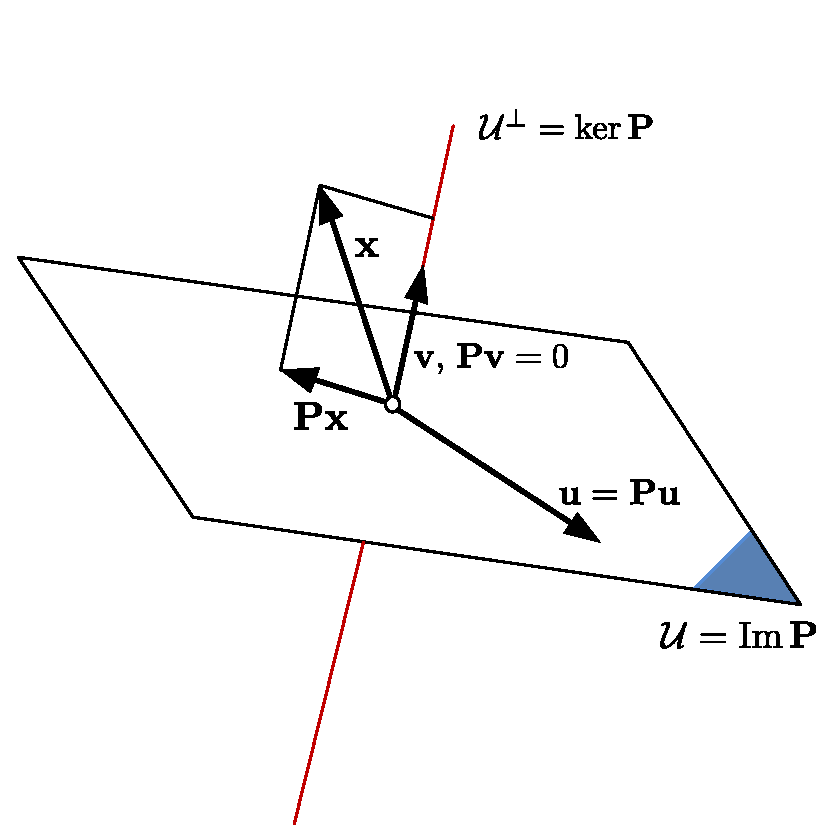
\includegraphics[width=0.7\linewidth]{MAI016.pdf}
    \captionof{figure}{K příkladu \ref{mai:exam012}}
    \label{MAI:FIG016}
    \par}        
\end{example}
      %---------------------------------------------------------------

      %---------------------------------------------------------------
        % !TeX spellcheck = cs_CZ


\begin{example}\label{mai:exam013}
  Určete spektrum matice a její spektrální poloměr následující matice
    \begin{equation*}\label{pr:spektrum_matice}
      \mathbf{A} =
        \begin{pmatrix}
          2  &  2    & 0 \\
         -3  & -3    & 5 \\
          0  & -0.25 & 2
        \end{pmatrix}
    \end{equation*}
  \textbf{Řešení}: Spektrum matice je množina všech jejích vlastních čísel. Spektrální poloměr 
  je maximum z absolutních hodnot vlastních čísel. Vlastní čísla určíme z charakteristické
  rovnice \(\det(\mathbf{A}-\lambda \mathbf{I})=0\).
    \begin{equation*}
      \textbf{A} - \lambda\textbf{I}=
        \begin{pmatrix}
          2-\lambda  &  2          & 0 \\
         -3          & -3-\lambda  & 5 \\
          0          & -0.25       & 2-\lambda
       \end{pmatrix}
    \end{equation*}
    \begin{align}
      \det(\mathbf{A}-\lambda \mathbf{I})                    &= 0           \nonumber\\
      (2-\lambda)
        \begin{pmatrix}
          -3-\lambda  &  5\\
             -0.25    &  2 - \lambda
        \end{pmatrix} -2\cdot
        \begin{pmatrix}
          -3       &  5\\
           0       &  2 - \lambda
        \end{pmatrix}                                        &= 0           \nonumber\\
      (2-\lambda)^2(-3-\lambda)+1.25(2-\lambda)+6(2-\lambda) &= 0           \nonumber\\
      (2-\lambda)[(2-\lambda)(-3-\lambda)+1.25+6]            &= 0           \nonumber\\
      (2-\lambda)(\lambda^2+\lambda+1.25)                    &= 0           \nonumber
    \end{align}
    \begin{equation*}
      \lambda_1 = 2, \quad\lambda_2 = -0.5+i, \quad\lambda_3=-0.5-i
    \end{equation*}
    \begin{itemize}
      \item Spektrum matice \(\mathbf{A}\) je \(\sigma(\mathbf{A})=\{2,-0.5+i,-0.5-i\}\).
      \item Spektrální poloměr \(\rho(\mathbf{A})=\max_i|\lambda_i|=2\).
    \end{itemize}

%    \attachfile[icon=Paperclip, description=Matlab Determine the spectrum of a matrix 
%      and its spectral radius]{../SRC/MAI/matlab/LA001.m}

\end{example}
      %---------------------------------------------------------------

      %---------------------------------------------------------------
        % !TeX spellcheck = cs_CZ
\begin{example}\label{mai:exam014}
  Určete vlastní čísla a vlastní vektory matice \(\mathbf{B} = \mathbf{A}^2 - 4\mathbf{A} + 
  9\mathbf{A}^{-1} - \mathbf{I}\), kde \(\mathbf{A}\) je matice \(\mathbf{A}= 
  \begin{pmatrix}1&0.5\\3.5&4\end{pmatrix}\).

  \textbf{Řešení}: (z předchozího příkladu víme, že \(\lambda_1=4.5, \lambda_2=0.5\)) a
   \(\mathbf{I}\) jednotková matice. Označme symbolem \(\lambda\) vlastní číslo matice 
   \(\mathbf{A}\) a nechť \(\mathbf{x}\) je příslušný vlastní vektor. Pak platí:
   \begin{itemize}
     \item Matice \(\mathbf{A}^2\) má vlastní čísla rovna \(\lambda^2\).
     \item Matice \(4\mathbf{A}\) má vlastní čísla rovna \(4\lambda\).
     \item Matice \(9\mathbf{A}^{-1}\) má vlastní čísla rovna \(\frac{9}{\lambda}\).
   \end{itemize}
   Matice \(\mathbf{B}=\mathbf{A}^2-4\mathbf{A}+9\mathbf{A}^{-1}-\mathbf{I}\) má vlastní čísla 
   ve tvaru  \(\lambda^2-4\lambda+\frac{9}{\lambda}-1\), vlastní vektory jsou stejné jako 
   vlastní vektory odpovídající vlastním číslům matice \(\mathbf{A}\). Tedy:
   \begin{equation*}
       \sigma(B)=\{4.5^2-4\cdot4.5+\frac{9}{4.5}-1,\quad
       0.5^2-4\cdot0.5+\frac{9}{0.5}-1\}=\{3.25, 15.25\}
   \end{equation*}
\end{example}
      %---------------------------------------------------------------


      %---------------------------------------------------------------
       % !TeX spellcheck = cs_CZ

\begin{example}\label{mai:exam002}
  Určete vlastní čísla a odpovídající vlastní vektory následují\-cích matic:
  \begin{equation*}
    \mathbf{A}=
      \begin{pmatrix}
        1   & 0.5\\
        3.5 & 4
      \end{pmatrix}, \quad
    \mathbf{B}=
      \begin{pmatrix}
        3   & -1 \\
        2.5 &  4 
      \end{pmatrix}
  \end{equation*}
  \textbf{Řešení}: Vlastní čísla určíme z charakteristické rovnice: \(\det(\mathbf{A} - 
  \lambda\mathbf{I}) = 0\). Vlastní vektory \(\mathbf{x_i}\) odpovídající vlastním číslům 
  \(\lambda_i\), jsou řešením homogenní soustavy rovnic \((\mathbf{A} - 
  \lambda_i\mathbf{I})\mathbf{x_i} = 0\).
  \begin{itemize}
    \item Vlastní čísla matice \textbf{A}:
      \begin{equation*}
           \textbf{A} - \lambda\textbf{I} =
             \begin{pmatrix}
                1-\lambda  &  0.5          \\
               -3.5        &  4-\lambda
             \end{pmatrix}
      \end{equation*}
      \begin{align*}
         \det(\mathbf{A}-\lambda\mathbf{I}) &= 0 \\
         (1-\lambda)(4-\lambda)-\frac{7}{4} &= 0 \\
         \lambda^2-5\lambda+\frac{9}{4}     &= 0
      \end{align*}
      \begin{equation*}
         \lambda_1 = 4.5,\quad \lambda_2 = 0.5
      \end{equation*}
  \end{itemize}

    \begin{itemize}
      \item Vlastní čísla matice \textbf{B}:
        \begin{equation*}
             \textbf{B} - \lambda\textbf{I}=
               \begin{pmatrix}
                 3-\lambda  & -1             \\
                 2.5        &  4-\lambda
               \end{pmatrix}
        \end{equation*}
        \begin{align*}
           \det(\mathbf{B}-\lambda\mathbf{I}) &= 0 \\
           (3-\lambda)(4-\lambda)+\frac{5}{2} &= 0 \\
           \lambda^2-7\lambda+\frac{29}{2}    &= 0
        \end{align*}
        \begin{equation*}
           \lambda_1 = \frac{7+3i}{2},\quad \lambda_2 = \frac{7-3i}{2}
        \end{equation*}
    \end{itemize}
  % matice A
  Vlastní vektor matice \(\mathbf{A}\) pro \(\lambda_1=4.5: (\mathbf{A} - 
  \lambda_1\mathbf{I})\mathbf{x_1} = 0 \Rightarrow\)
  \begin{align*}
    \begin{pmatrix}
       1  -4.5  &  0.5     \\
      -3.5      &  4-4.5
    \end{pmatrix}
    &\sim
    \begin{pmatrix}
      -3.5  &  0.5         \\
      -3.5  & -0.5
    \end{pmatrix}          \\
    \Rightarrow\mathbf{x_1} &=
    \begin{pmatrix}
      1 \\ 7
    \end{pmatrix}
    \, r, r\in\mathbb{R}, r\neq0
  \end{align*}
  Vlastní vektor matice \(\mathbf{A}\) pro \(\lambda_2=0.5: (\mathbf{A} - 
  \lambda_1\mathbf{I})\mathbf{x_2}=0 \Rightarrow\)
  \begin{align*}
    \begin{pmatrix}
       1  -0.5  &  0.5   \\
      -3.5      &  4-0.5
    \end{pmatrix}
    &\sim
    \begin{pmatrix}
       0.5  &  0.5       \\
       3.5  &  3.5
    \end{pmatrix}        \\
    \Rightarrow\mathbf{x_2} &=
    \begin{pmatrix}
      -1 \\ 1
    \end{pmatrix}
    \, r, r\in\mathbb{R}, r\neq0
  \end{align*}
  % matice B
  Vlastní vektor matice \(\mathbf{A}\) pro \(\lambda_1=\frac{7+3i}{2}: (\mathbf{B} - 
  \lambda_1\mathbf{I})\mathbf{x_1}=0 \Rightarrow\)
  \begin{align*}
    \begin{pmatrix}
       3 - \frac{7+3i}{2}            & -1                                     \\
       \frac{5}{2}                   &  4 - \frac{7+3i}{2}
    \end{pmatrix}
    \sim
    \begin{pmatrix}
      -\frac{1}{2}-\frac{3}{2}i      &  -1                                     \\
      \frac{5}{2}                    & \frac{1}{2}-\frac{3}{2}i
    \end{pmatrix}
    \sim \\
    \begin{pmatrix}
      -\frac{10}{4}                  &-\left(\frac{1}{2} -\frac{3}{2}i\right)  \\
      \frac{5}{2}                    & \frac{1}{2}-\frac{3}{2}i
    \end{pmatrix}
    \sim
    \begin{pmatrix}
      -5                           &-\left(1-3i\right)                         \\
       5                           & \left(1-3i\right)
    \end{pmatrix}
    \rightarrow \\
    \mathbf{x_1}=
    \begin{pmatrix}
      -1+3i \\ 5
    \end{pmatrix}
    \, r, r\in\mathbb{C}, r\neq0
  \end{align*}
  Vlastní vektor matice \(\mathbf{B}\) pro \(\lambda_2=\frac{7-3i}{2}: (\mathbf{B} - 
  \lambda_1\mathbf{I})\mathbf{x_2}=0 \Rightarrow\)
  \begin{align*}
    \begin{pmatrix}
       3  - \frac{7-3i}{2}       &  -1                                     \\
      \frac{5}{2}                &  4 - \frac{7-3i}{2}
    \end{pmatrix}
    \sim
    \begin{pmatrix}
      -\frac{1}{2}+\frac{3}{2}i  &  -1                                     \\
      \frac{5}{2}                & \frac{1}{2}+\frac{3}{2}i
    \end{pmatrix}
    \\sim \\
    \begin{pmatrix}
      -\frac{10}{4}              &-\left(\frac{1}{2} +\frac{3}{2}i\right)  \\
      \frac{5}{2}                & \quad\frac{1}{2}+\frac{3}{2}i
    \end{pmatrix}
    \sim
    \begin{pmatrix}
      -5                         &-\left(1+3i\right)                       \\
       5                         & \quad\left(1+3i\right)
    \end{pmatrix}
    \rightarrow\\
    \mathbf{x_2}=
    \begin{pmatrix}
      -1-3i \\ 5
    \end{pmatrix}
    \, r, r\in\mathbb{C}, r\neq0
  \end{align*}
\end{example}
%---------------------------------------------------------------
\lstinputlisting{../src/MAI/matlab/LA001.m}
\begin{lstlisting}[caption=Výpis programu pro ověření výpočtu vlastních čísel matic programem
  Matlab.]
\end{lstlisting}
%---------------------------------------------------------------
      %---------------------------------------------------------------

  %====================== Kapitola: Polynomy ======================================================
  \section{Polynomy}
      \begin{definition}\label{def_rov_poly}\textbf{Rovnost dvou polynomů}:
        Řekneme, že dva polynomy \(f(x)=a_nx^n+a^{(n-1)}x_{(n-1)}+\ldots+a_1+a_0\) a
        \(g(x)=b_mx^m+b^{(m-1)}x_{(m-1)}+\ldots+b_1+b_0\) stupňů \(n\) a \(m\) se sobě 
        \textbf{rovnají} právě tehdy, když \(m=n\) a \(a_0=b_0\), \(a_1=b_1\), 
        \(a_{(n-1)}=b_{(m-1)}\), \(a_n=b_m\). V tomto případě také říkáme, že mnohočleny \(f(x)\) a 
        \(g(x)\) jsou \textbf{totožné}.
      \end{definition}
      \begin{lemma}\label{la:eq_eqv_poly}
        Jestliže mnohočleny \(f(x)\) a \(g(x)\) jsou dva polynomy stupně \(n\)-tého a jestliže pro 
        \(n+1\) různých reálných nebo komplexních čísel \(x\) platí \(f(x)=g(x)\), potom jsou 
        polynomy \textbf{totožné}.
      \end{lemma}
      
    \subsection{Rozklad ryze racionální funkce na parci\-ální zlomky}

      %---------------------------------------------------------------
       % !TeX spellcheck = cs_CZ
\begin{example}\label{mai:exam015}
  Rozložte na parciální zlomky lomenou racionální funkci \((x):y=\frac{7x+8}{x^2+x-2}\).
  \newline\textbf{Řešení:} Nejprve vypočteme nulové body jmenovatele:
  \begin{align*} 
     x^2+px+q &=(x-u)(x-v) = x^2-(u+v)x+uv            \\
              &\rightarrow p=-(u+v),\quad q=uv
  \end{align*}
  Kořenové činitele  \(x^2+x-2\rightarrow x_1=1, x_2=-2\) zvolíme za jmenovatele parciálních
  zlomků a rozklad hledáme ve tvaru \(\frac{7x+8}{x^2+x-2}=\frac{A}{x-1}+\frac{B}{x+2}\)
  kde \(A\), \(B\) jsou neznámé konstanty. Tyto konstanty určíme tak, aby rozklad platil pro 
  každé \(x\in\mathcal{R}-\{1,-2\}\). Po jednoduché úpravě dostaneme rovnost dvou polynomů
  \(7x+8=(A+B)x+2A-B\). Podle \ref{la:eq_eqv_poly} se musí rovnat koeficienty u \(x\) a absolutní 
  členy obou stran poslední rovnice \(\Rightarrow\) dostaneme soustavu rovnic pro určení \(A\) a 
  \(B\) ve tvaru:
  \begin{align}
    % \nonumber to remove numbering (before each equation)
    7 &= A+B  \nonumber \\ 
    8 &= 2A+B \label{la:eq_parc_example}   
  \end{align}
  dostáváme \(A=5,\quad B=2\). Postup, který jsme užili, nazýváme \textbf{Metodou neurčitých 
  koeficientů}.
  
  Pro určení koeficientů \(A\), \(B\) se užívají také jiné postupy, např. dosazování
  kořenů jmenovatele, která je výhodná zejména v případech, kdy jmenovatel lomené racionální
  funkce má jednoduché kořeny. Postupujeme tak, že rov. \ref{la:eq_parc_example} násobíme
  součinem kořenových činitelů \((x-1)(x+2)=x^2+x-2\) a dostaneme rovnici 
  \(7x+8=A(x+2)+B(x-1)\) pro určení koeficientů \(A\), \(B\) dosazováním kořenů.
    \begin{align*}
      % \nonumber to remove numbering (before each equation)
      x=-2 &\rightarrow       -14+8=B(-2-1)      \rightarrow B=2\\
      x=+1 &\rightarrow  \,\,\,+7+8=A(1+2)\quad  \rightarrow A=5
    \end{align*}
\end{example}
      %---------------------------------------------------------------
      
  %==================== Kapitola: Vektorové prostory ===============================================
  \section{Vektorové prostory se skalárním součinem}
    \subsection{Ortogonální doplňky}
      Nechť \(U\) je podprostor vektorového prostoru \(V\). Ortogonální doplněk $U^\bot$ obsahuje 
      všechny vektory, které jsou kolmé ke každému vektoru z \(U\), neboli \(\forall\vec{v}\in 
      U^\bot\quad \forall\vec{u}\in U\quad \vec{u}\bot\vec{v}\) což lze vyjádřit pomocí skalárního 
      součinu \(\vec{u}\cdot\vec{v} = 0\)
  
      Ortogonální doplněk \(U^\bot\) k podprostoru \(U = \langle\vec{u}_1,\ldots,\vec{u}_k\rangle\) 
      tedy hledáme jako řešení homogenní soustavy rovnic
      \begin{equation*}
        \left(
          \begin{array}{c|c}
             \vec{u}_1  &   0      \\
             \cdots     &  \vdots  \\
             \vec{u}_k  &   0
          \end{array}
        \right),
      \end{equation*}
      nuly na pravé straně při výpočtu zpravidla vynecháváme. Připomeňme také vztah
      \begin{equation}\label{LA:eq_dim_doplnek}
         \dim U + \dim U^\bot = \dim V
      \end{equation}

      %---------------------------------------------------------------
        % !TeX spellcheck = cs_CZ
% Musilova2009MA1

\begin{example}\label{mai:exam011}
  Zjistěte ortogonální doplněk \(\langle(1,-3,2),(2,1,5)\rangle\bot^.\). (Zdroj:
  \cite[s.~3]{MosnaMA3})
  \newline\textbf{Řešení}:
  Hledáme vektor \((x, y, z)\), jehož skalární součin je se zadanými vektory roven nule. Budeme 
  tedy řešit (úpravou na Gaussův tvar pomocí elementárních úprav) homogenní soustavu rovnic
  zadanou maticí
  \begin{equation*}
     \left(
       \begin{array}{ccc|c}
          1  &  -3  & 2 & 0 \\
          2  &   1  & 5 & 0
       \end{array}
     \right)\sim
     \left(
       \begin{array}{ccc|c}
          1  &  -3  & 2 & 0 \\
          0  &   7  & 1 & 0
       \end{array}
     \right)\
  \end{equation*}
  Odtud dostáváme \(z = \alpha\), \(7y + z = 0\) \(\Rightarrow\) \(y = -\frac{1}{7}\alpha\), \(x
  +\frac{3}{7}\alpha + 2\alpha = 0\) \(\Rightarrow\) \(x = -\frac{17}{7}\) neboli 
  \begin{equation*}
  (x, y, z) =\alpha\left(-\frac{17}{7}, -\frac{1}{7}, 1\right) = \alpha(17, 1, -7)
  \end{equation*}

  V dalších příkladech budeme nuly na pravé straně soustavy vynechávat a upravovat na
  výhodnější tvar
  \begin{align*}
       \begin{pmatrix}
          1  &  -3  & 2  \\
          2  &   1  & 5
       \end{pmatrix}
       & \sim
       \begin{pmatrix}
          1  &  -3  & 2 \\
          0  &   7  & 1
       \end{pmatrix}
       \sim                         \\
       \begin{pmatrix}
          1  &   0  & \frac{17}{7}  \\
          0  &   7  & 1
       \end{pmatrix}
       & \sim
       \begin{pmatrix}
          7  &   0  & 17 \\
          0  &   7  & 1
       \end{pmatrix}.
  \end{align*}
  Odtud již snadno zjistíme, že vektor \((x, 1, -7)\) jistě vyhovuje druhé rovnici. Dosadíme-li ho 
  do první rovnice, dostaneme \(7x + 17\cdot(-7) = 0\) a \(x = 17\).

  Hledaný ortogonální doplněk je tedy lineární obal $$\langle(17, 1, -7)\rangle^\bot.$$
  
    {\centering
     \captionsetup{type=figure}
    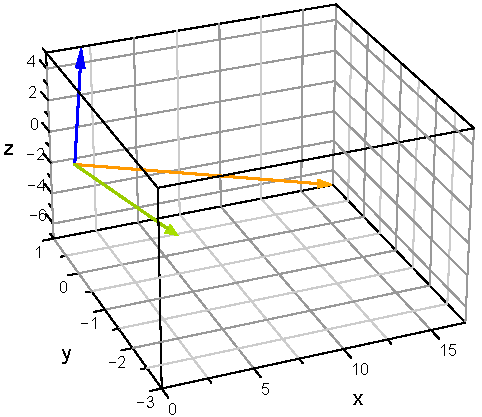
\includegraphics[width=0.8\linewidth]{ort_doplnek_exam01.pdf}
    \captionof{figure}[Ortogonální doplněk]{Vizualizace vektorového prostoru a jeho    
             ortogonálního doplňku pomocí sw MatLab - MuPAD příkazem:\newline
             \texttt{plot(plot::Arrow3d([1,-3,2]), plot::Arrow3d([2,1,5]), 
             plot::Arrow3d([17,1,-7]))}}
    \label{LA:fig_ort01}
    \par}
\end{example}

      %---------------------------------------------------------------
  
      Výsledek předchozího příkladu \ref{mai:exam011} lze interpretovat tak, že jsme našli všechny 
      vektory, které jsou kolmé na rovinu určenou vektory ze zadání. Rovina je útvar       
      dvojrozměrný a protože prostor všech vektorů je trojrozměrný, musí nutně mít podprostor 
      ortogonálních vektorů ve shodě se vztahem \ref{LA:eq_dim_doplnek} pouze jednu dimenzi. Vše 
      je dobře patrné z obr. \ref{LA:fig_ort01}

} % tikzset
%---------------------------------------------------------------------------------------------------
\printbibliography[title={Seznam literatury}, heading=subbibliography]
\addcontentsline{toc}{section}{Seznam literatury}
%------------------- Differential calculus --------------------------------------------------------
  %     Differential calculus
%--------------------------------------------------------------------------------------------------
% file Diff_calc.tex
%--------------------------------------------------------------------------------------------------
\chapter{Limita a spojitost funkce}\label{MA1:chap_Limita}
\minitoc
\newpage
  %================Podkapitola: Reálná funkce =====================================================
  \section{Reálná funkce}
    %----------------------------------------------------------------------------------------------
    \subsection{Pojem funkce}
    %----------------------------------------------------------------------------------------------
    \subsection{Graf funkce. Různé způsoby zadání funkce}
      Každé funkci můžeme přiřadit její graf. 
      \textbf{Grafem funkce} $f:A\rightarrow\realset,\ A\subset\realset$, rozumíme množinu všech bodů 
      euklidovské roviny, jejíž souřadnice $x$, $y$ v dané kartézské soustavě souřadnic vyhovuje rovnice 
      \begin{equation}\label{MAI:eq_graf04}
        y=f(x). 
      \end{equation}  
      
      Grafem funkce může v jednodušších případech posloužit jako prostředek k získání názorné       
      \textquotedblleft představy\textquotedblright. Grafy některých funkcí jsou \textquotedblleft 
      křivky\textquotedblright\, (intuitivním smyslu tohoto slova). Avšak u některých funkcí názorná 
      představa grafu selhává. Vezmeme-li např. Dirichletovu funkci z odst. **, snadno zjistíme, že její graf 
      nemůžeme sestrojit (byly by to \textquotedblleft dvě rovnoběžné přímky $y=0$ a $y=1$ s nekonečným 
      množstvím mezer\textquotedblright)
      
      Zadat funkci znamená udat její definiční obor a \textquotedblleft zobrazovací předpis 
      \textquotedblright, tj pravidlo (formulované slovně či v používaném matematickém jazyku), 
      podle něhož můžeme jednoznačným způsobem rozhodnout, jaká funkční hodnota odpovídá libovolně 
      zvolenému číslu z definičního oboru. Definičním oborem bývá často interval nebo sjednocení 
      intervalů. Není-li definiční obor udán, rozumíme jím množinu všech reálných čísel, pro něž je 
      příslušný předpis definován. Tuto množinu nazýváme \textbf{přirozeným (též maximálním) 
      definičním oborem funkce}. Je to tzv. \emph{existenční obor} výrazu, jímž je funkce definována 
      \cite[s.~84]{Brabec1989}.
      
      Například funkce $f: \realset\rightarrow\realset,\ f(x)=x^2$, můžeme vyjádřit bez udání definičního  
      oboru 
      $\realset$ vztahem 
      \begin{equation*}
        f: y=x^2,
      \end{equation*}
      neboť předpis $y=x^2$ má smysl pro každé reálné číslo $x$. Avšak u funkce 
      $g:\langle0,1\rangle\rightarrow\realset,\ g(x)=x^2,$ je nutné v zápisu funkce definiční obor 
      $\langle0,1\rangle$ uvést, píšeme tedy   
      \begin{equation*}
        g: y=x^2, \quad x\in\langle0,1\rangle.
      \end{equation*}
      Zobrazovací předpis, kterým je funkce zadána, může být rozmanitý. Nejčastěji a pro účely matematické 
      analýzy nejvhodnější je \emph{analytické zadání vzorcem}, tj. rovnicí tvaru $y=f(x)$ nebo několika 
      takovými rovnicemi platnými pro různé části definičního oboru. Přitom v rovnici $y=f(x)$ je na pravé 
      straně nějaký správně definovaný výraz obsahující nejvýše poměnnou $x$ a nabývající jednoznačné hodnoty 
      pro danou hodnotu proměnné $x$.

      \begin{example}\label{MAI:exam01} 
        Vzorcem $f(x)=\sqrt{1-x}$ je dána funkce, jejímž přirozeným oborem je interval $(-\infty,1\rangle$ 
        (uvažme, že výraz $\sqrt{1-x}$ je definován v reálném oboru, je-li $1-x\geq0$). Graf této funkce 
        je část paraboly, jejíš osou je osa $x$, viz obr. \ref{MAI:fig_diff_app_03}.
        %----------------------------------
        % image: MAI_diff_app_03.tex label: \label{MAI:fig_diff_app_03}
           % \documentclass{article}
% \usepackage{xltxtra} 
% \usepackage{tikz}
% \usetikzlibrary{decorations.markings}
% \usetikzlibrary{intersections}
% \usepackage{subfigure} 
% \usetikzlibrary{calc}
% 
% \newcommand{\MyXYcross}{%
%           \draw[name path=axeX,->] (\xmin,\zero) -- (\xmax,\zero)   node[right] {$x$} coordinate(x axis);
%           \draw[name path=axeY,->] (\phase,\ymin) -- (\phase,\ymax) node[left]  {$y$} coordinate(y axis);
%           \path[name intersections={of=axeX and axeY, name=pocatek}]; 
%           \node[below left] at (pocatek-1) {$0$};
%           \draw[fill=white] (pocatek-1) circle(2pt);  
% }
%\begin{document}

  \begin{figure}[htb]  
    \centering
        \def\xmin{-160}
        \def\xmax{100}
        \def\ymin{-15}
        \def\ymax{+100}
        \def\zero{0}
        \def\phase{0}
      \begin{tikzpicture}
        \begin{scope}[draw=black,line join=round, miter limit=4.00,line width=0.5pt,y=1pt,x=1pt] 
          \MyXYcross;   
        \end{scope}
        
        \begin{scope}[domain=-2:1, line join=round, miter limit=4.00,line width=0.5pt, 
                      x=50pt,y=50pt, xshift=0, yshift=0]    
         \draw[color=red] plot[id=myfce, samples=2000, smooth] function{sqrt(1-x)}; 
         % 
         \foreach \x/\xtext in {-1/1, -2/2, -3/3}
            \draw[shift={(\x,0)}] (0pt,2pt) -- (0pt,-2pt) node[below] {$\xtext$};
            
         \node at(2,1.2) [left, fill=white] {$f(x): y=\sqrt{1-x}$}; %   
         \draw[fill=black] (1,0) node[below] {$1$} circle(1pt);
          \draw[fill=black] (0,1) circle(1pt);  
          \node at (0,1) [left] {$1$};        
        \end{scope}  
      \end{tikzpicture}
    \caption{Graf funkce $y=\sqrt{1-x}$ je část paraboly, jejíž osou je osa $x$}\label{MAI:fig_diff_app_03}
  \end{figure}
  
%\end{document}  
        %----------------------------------         
      \end{example}   
      \begin{example}\label{MAI:exam07} 
        Funkce je dána vzorcem 
        \begin{equation*}
          f(x):y=\abs{x}.
        \end{equation*} 
        Přirozeným definičním oborem této funkce je množina $\realset$. Táž funkce může být dána i vzorcem
        \begin{equation*}
          f(x):y=\sqrt{x},
        \end{equation*}    
        nebo dvěma rovnicemi
        \begin{equation*}
          f(x):y=
             \begin{cases}
                 x & \text{je-li} x \geq 0. \\
                -x & \text{je-li} x < 0,
             \end{cases}                 
        \end{equation*}  
        což je zřejmé, uvědomíme-li si jak je definována absolutní hodnota. Graf funkce je na obr. 
        \ref{MAI:fig_diff_app_05}.
        %----------------------------------
        % image: MAI_diff_app_05.tex label: \label{MAI:fig_diff_app_05}
           % \documentclass{article}
% \usepackage{xltxtra} 
% \usepackage{tikz}
% \usetikzlibrary{decorations.markings}
% \usetikzlibrary{intersections}
% \usepackage{subfigure} 
% \usetikzlibrary{calc}
% \usepackage{amsmath, amsthm, amssymb, amsfonts, amsbsy}
% 
% \newcommand{\abs}[1]{\left\lvert#1\right\rvert} 
% \newcommand{\MyXYcross}{%
%           \draw[name path=axeX,->] (\xmin,\zero) -- (\xmax,\zero)   node[right] {$x$} coordinate(x axis);
%           \draw[name path=axeY,->] (\phase,\ymin) -- (\phase,\ymax) node[left]  {$y$} coordinate(y axis);
%           \path[name intersections={of=axeX and axeY, name=pocatek}]; 
%           \node[below left] at (pocatek-1) {$0$};
%           \draw[fill=white] (pocatek-1) circle(2pt);  
% }
% \begin{document}

  \begin{figure}[htb]  
    \centering
        \def\xmin{-100}
        \def\xmax{100}
        \def\ymin{-15}
        \def\ymax{+100}
        \def\zero{0}
        \def\phase{0}
      \begin{tikzpicture}
        \begin{scope}[draw=black,line join=round, miter limit=4.00,line width=0.5pt,y=1pt,x=1pt] 
          \MyXYcross;   
        \end{scope}
        
        \begin{scope}[domain=-1:1, line join=round, miter limit=4.00,line width=0.5pt, 
                      x=50pt,y=50pt, xshift=0, yshift=0]    
          \node at(2,1.2) [left, fill=white] {$f(x): y=\abs{x}$};   %                         
          \draw[color=red] plot[id=myfce, samples=2000, smooth] function{abs(x)}; % 
          
          \foreach \x/\xtext in {-1/1, 1/1}
            \draw[shift={(\x,0)}] (0pt,2pt) -- (0pt,-2pt) node[below] {$\xtext$};                 
        \end{scope}  
      \end{tikzpicture}
    \caption{Graf funkce $y=\abs{x}$}\label{MAI:fig_diff_app_05}
  \end{figure}
  
%\end{document}  
        %----------------------------------         
      \end{example}  
      Funkce může být analyticky zadána i jinak než vzorcem $y=f(x)$. časté je \textbf{parametrické 
      vyjadřování}, tj. vyjádření dvojicí rovnic 
      \begin{equation}\label{MAI:eq_graf02}
        x=\varphi(t),\ y=\psi(t),\ t\in J,
      \end{equation}
      kde $\varphi, \psi$ jsou funkce definované na množině $J$ ($\ J$ bývá obvykle interval). Proměnná $t$ 
      se nazývá \emph{parametr}: má zde pomocný význam. Zajímá nás totiž vztah mezi $x$ a $y$. Rovnice 
      \ref{MAI:eq_graf02} definuje relaci $f\subset\realset\times\realset=\realset^2$:
      \begin{equation}\label{MAI:eq_graf03}
        f = \{(x,y)\in\realset^2; \text{ existuje } t\in J \text{ tak, že } x=\varphi(t),\ y=\psi(t)\}.
      \end{equation}      
      Tato relace může být za určitých podmínek jednoznačná tj. je funkcí z $\realset$ do $\realset$. 
      V tomto případě říkáme, že funkce $f$ je \emph{definována parametricky rovnicemi \ref{MAI:eq_graf02}}
      
      \begin{example}\label{MAI:exam02}
        Rovnice $x=\cos t,\ y=\sin t\quad t\in\langle0,\pi\rangle$, definují parametricky funkci 
        \begin{equation}
          f: y= \sqrt{1-x^2}, \quad x\in\langle-1,1\rangle,
        \end{equation}
        jejíž grafem je polokružnice, ležící v horní polorovině $\{(x,y)\in\realset^2, y\geq0\}$.
        %----------------------------------
        % image: MAI_diff_app_04.tex label: \label{MAI_fig_diff_app_04}
           % \documentclass{article}
% \usepackage{xltxtra} 
% \usepackage{tikz}
% \usetikzlibrary{decorations.markings}
% \usetikzlibrary{intersections}
% \usepackage{subfigure} 
% \usetikzlibrary{calc}
% 
% \newcommand{\MyXYcross}{%
%           \draw[name path=axeX,->] (\xmin,\zero) -- (\xmax,\zero)   node[right] {$x$} coordinate(x axis);
%           \draw[name path=axeY,->] (\phase,\ymin) -- (\phase,\ymax) node[left]  {$y$} coordinate(y axis);
%           \path[name intersections={of=axeX and axeY, name=pocatek}]; 
%           \node[below left] at (pocatek-1) {$0$};
%           \draw[fill=white] (pocatek-1) circle(2pt);  
% }
% \begin{document}

  \begin{figure}[htb]  
    \centering
        \def\xmin{-100}
        \def\xmax{100}
        \def\ymin{-15}
        \def\ymax{+100}
        \def\zero{0}
        \def\phase{0}
      \begin{tikzpicture}
        \begin{scope}[draw=black,line join=round, miter limit=4.00,line width=0.5pt,y=1pt,x=1pt] 
          \MyXYcross;   
        \end{scope}
        
        \begin{scope}[domain=-1:1, line join=round, miter limit=4.00,line width=0.5pt, 
                      x=50pt,y=50pt, xshift=0, yshift=0]    
          \node at(2,1.2) [left, fill=white] {$f(x): y=\sqrt{1-x}$};    %                         
          \draw[color=red] plot[id=myfce, samples=200, smooth] function{sqrt(1-x*x)}; %    
          \draw[fill=black] (+1,0) node[below] {$1$}  circle(1pt);
          \draw[fill=black] (-1,0) node[below] {$-1$} circle(1pt);
          \draw[fill=black] (0,1) circle(1pt);  
          \node at (0,1) [left] {$1$};        
        \end{scope}  
      \end{tikzpicture}
    \caption{Graf funkce $y=\sqrt{1-x}$ je polokružnice}\label{MAI:fig_diff_app_04}
  \end{figure}
  
%\end{document}  
        %----------------------------------         
      \end{example}
      Blíže se parametrickým zadáním funkce budeme zabívat v kapitole \ref{chap:Apl_dif_poc} (Aplikace 
      diferenciálního počtu).
      
      Funkce může být někdy zadána též rovnicí tvaru 
      \begin{equation}\label{MAI:eq_graf01}
        F(x,y) = 0.
      \end{equation}
      Přitom $F$ je funkce dvou proměnných, tj. zobrazení z $\realset^2\rightarrow\realset$. Kromě rovnice 
      \ref{MAI:eq_graf01} může být dána ještě podmínka, aby bod $(x,y)$ patřil k některé množině 
      $M\subset\realset^2$. Rovnicí \ref{MAI:eq_graf01} je definován opět jakási relace 
      $f\subset\realset\times\realset$,
      \begin{equation}
        f = \{(x,y)\in\realset^2,\quad F(x,y)=0 \}
      \end{equation}
      (případně $f = \{(x,y)\in\realset^2,\ F(x,y)=0,\ (x,y)\in M \}$), zajímá nás, kdy tato relace je 
      funkcí z $\realset$ do $\realset$. Říkáme pak, že funke $f$ je dána \textbf{implicitně} uvedenou 
      rovnicí \ref{MAI:eq_graf01} (příp. rovnicí \ref{MAI:eq_graf01} a podmínkou $(x,y)\in M$). 
      Naproti tomu zadání funkce ve tvaru 
      $y=f(x)$ nazýváme \textbf{explicitním}.
      
      \begin{example}\label{MAI:exam03} 
        Rovnicí $x+2y-3=0$ je implicitně definována funkce $f:y=-\dfrac{1}{2}x+\dfrac{3}{2}$.
      \end{example}
      \begin{example}\label{MAI:exam04} 
        Rovnicí $x^2+y^2=1$ a podmínkou $y\geq0$ je definována implicitní funkce z příkladu \ref{MAI:exam02}. 
        Relace $\{(x,y)\in\realset^2;\ x^2+y^2=1\}$ není ovšem jednoznačná, každé hodnotě $x\in(-1,1)$ 
        odpovídají dvě hodnoty $y: y_1=\sqrt{1-x^2}$, $y: y_2=-\sqrt{1-x^2}$. Podmínkou $y\geq0$ druhou 
        hodnotu vylučujeme. Místo podmínky $y\geq0$ bychom mohli uvést i jiné podmínky, aby rovnice 
        $x^2+y^2=1$ určovala implicitní funkci.   
      \end{example}
      
      Vyšetřování podminek, při nichž rovnice $F(x,y)=0$ je definována funkce $f$, se obvykle provádí 
      metodami matematické analýzy funkce více proměnných. 
      
      Funkce může být někdy dána tabulkou, tj. dvojicemi hodnot argumentu a funkce, což bývá obvyklé při 
      zjišťování závislosti veličin měřením. Proměnná $x$ se v tomto případě mění \textquotedblleft 
      diskrétně\textquotedblright. Je zřejmé, že tímto způsobem můžeme definovat úplně jen tehdy, je-li 
      definiční obor konečná množina. Tabulku však používáme i v jiných případech, zejména chceme-li vyznačit 
      pomocí ní, některé hodnoty, 
      které nás z nějakého důvodu přednostně zajímají. 
      
      V technických aplikacích bývá funkce dána graficky. Z grafu můžeme ovšem funkční hodnoty určit pouze 
      přibližně. Pro další matematické zpracování je grafické zadání nejméně vhodné, i když jeho praktický 
      význam nelze popřít. 
      
      Speciálním případem reálných funkcí jedné realné proměnné jsou \emph{posloupnosti reálných čísel}. 
         
    %----------------------------------------------------------------------------------------------        
    \subsection{Některé zvláštní vlastnosti funkcí}\label{MA1:subsec_vlastnosti_funkce}
      \subsubsection{Omezená funkce}
        \begin{definition}\label{MA1:def_lim01}
          Funkci $f$ nazýváme shora (zdola) omezenou na množině $A\subset D(f)$, je-li shora (zdola) omezená 
          množina funkčních hodnot $f(A)$. Je-li funkce $f$ omezená shora i zdola na množině $A$, pak ji 
          nazýváme omezenou na množině $A$. Je-li $A=D(f)$, nazýváme funkci omezenou. Viz kniha 
          \cite[s.~87]{Brabec1989}       
        \end{definition}
        Funkce $f$ je omezená na množině $A$, právě když existuje číslo $K>0$ tak, že platí
        $$|f(x)|\leq K \qquad \text{pro každé } x\in A$$
        neboli
        $$-K\leq f(x) \leq K \qquad \text{pro každé } x\in A.$$
        \begin{example}\label{MAI:exam05}
          Funkce $f:y=\frac{1}{x^2+1}$ je omezená. Platí totiž $$\left|\frac{1}{x^2+1}\right|=\frac{1}{x^2+1}\leq1 \qquad \text{pro všechna }x\in\realset.$$ Zdola
          je tato funkce omezena dokonce číslem $0$.  
        \end{example}
        \begin{itemize}
          \item Je-li funkce $f$ shora omezená na množině $A$, existuje konečné \emph{supremum} $\sup f(A)$. 
                Toto číslo nazýváme \emph{supremem funkce $f$ na množině $A$} a označujeme je též $\sup_{x\in 
                A}f(A)$ nebo $\sup\{f(x), x\in A\}$.
          \item Je-li funkce $f$ zdola omezená na množině $A$, existuje konečné \emph{infimum} $\inf(A)$,    
                které nazýváme \emph{infimum funkce $f$ na množině $A$} a označujeme je též $\inf_{x\in 
                A}f(A)$ nebo $\inf\{f(x), x\in A\}$. 
          \item Není-li funcke $f$ shoda (zdola) omezená na množině $A$, pak je ovšem $\sup_{x\in A}    
                f(x)=+\infty$ ($\sup_{x\in A} f(x)=-\infty$).
          \item Má-li množina $f(A)$ největší (nejmenší) prvek, pak toto číslo nazýváme největší 
                (nejmenší hodnotou funkce $f$  na množině $A$ (je-li $A = f(f)$, též absolutním maximem, 
                resp. absolutním minimem funkce $f$) a značíme je $\max_{x\in A} f(x)$ ($\min_{x\in A} 
                f(x)$). V tomto případě existuje takové číslo $x_0\in A$, že $f(x_0)=\max_{x\in A}f(x)$ 
                ($f(x_0)=\min_{x\in A}f(x)$). Pro všechna $x\in A$ tedy platí $f(x)\leq f(x_0)$ 
                ($f(x)\geq f(x_0)$). Je zřejmé, že největší (nejmenší) hodnota funkce $f$ na množině $A$, 
                pokud existuje je současně supremem (infimem) funkce $f$ na $A$.
        \end{itemize}
        \begin{example}\label{MAI:exam06}
          Pro funkci z příkladu \ref{MAI:exam05} platí:
          \begin{equation}
            \sup_{x\in\realset}=\frac{1}{x^2+1}=\max_{x\in\realset}=\frac{1}{x^2+1}=1; \qquad \inf_{x\in\realset}=\frac{1}{x^2+1}=0,
          \end{equation}
          tato funkce však nenabývá v definičním oboru $\realset$ nejmenší hodnoty, neboť je stále 
          $\dfrac{1}{x^2+1}>0$. To, že infimum je $0$, dokážeme takto: Zvolíme-li libovolně $\varepsilon>0$, 
          pak snadno zjistíme, že existuje $x$, pro níž $\dfrac{1}{x^2+1}<\varepsilon$:
          \begin{align*}
            1                  &< \varepsilon(x^2+1) \\
            \frac{1}{\epsilon} &< x^2+1 \Rightarrow \sqrt{\frac{1}{\epsilon}-1} < x
          \end{align*} 
          %----------------------------------
          % image: MAI_rolle_01.tex label: \label{MAI:fig_diff_app_02}
            % \documentclass{article}
% \usepackage{tikz}
% \usetikzlibrary{decorations.markings}
% \usetikzlibrary{intersections}
% \usepackage{subfigure} 
% \usetikzlibrary{calc}
% 
% \newcommand{\MyXYcross}{%
%    \draw[name path=axeX,->] (\xmin,\zero) -- (\xmax,\zero)   node[right] {$x$} coordinate(x axis);
%    \draw[name path=axeY,->] (\phase,\ymin) -- (\phase,\ymax) node[left]  {$y$} coordinate(y axis);
%    \path[name intersections={of=axeX and axeY, name=pocatek}]; 
%    \node[below left] at (pocatek-1) {$0$};
%    \draw[fill=white] (pocatek-1) circle(2pt);  
% }
%  \begin{document}
 
  \begin{figure}[htb]  
    \centering
        \def\xmin{-150}
        \def\xmax{150}
        \def\ymin{-15}
        \def\ymax{+90}
        \def\zero{0}
        \def\phase{0}
	  \begin{tikzpicture}
		\begin{scope}[draw=black,line join=round, miter limit=4.00,line width=0.5pt,y=1pt,x=1pt] 
          \MyXYcross;	
        \end{scope}
		
        \begin{scope}[domain=-2.5:2.5, line join=round, miter limit=4.00,line width=0.5pt, 
		              x=50pt,y=50pt, xshift=0, yshift=0]		
		  \draw[name path=fce, color=blue, smooth]   
		      plot[mark=triangle*] (\x,{1/(\x*\x+1)}); % 
		  \node at(2.5,1) [left, fill=white] {$f(x):y=\frac{1}{1+x^2}$};	
          \draw[dashed] (0,0.5) node[left] {$\frac{1}{2}$} -- ++(1,0) -- ++(0,-0.5) node[below] {$1$} ;
          \draw[fill=black] (1,0.5) circle(1pt);
          \draw[fill=black] (0,1) circle(1pt);	
          \node at (0,1) [left] {$1$};		  
		\end{scope}  
	  \end{tikzpicture}
    \caption{ }\label{MAI:fig_diff_app_02}
  \end{figure}
  
% \end{document}  
          %----------------------------------           
          Neexistuje tedy kladné číslo, jíž by bylo dolní mezí množiny funkčních hodnot, takže infimum je $0$. Graf funkce $f$ je na obr. \ref{MAI:fig_diff_app_02}.
        \end{example}
       
      \subsubsection{Monotonní funkce}
        \begin{definition}\label{MA1:def_lim02}
          Funkci $f$ nazýváme \textbf{rostoucí (klesající)} na množině $A\subset D(f)$, jestliže pro každé 
          dva body $x_1, x_2\in A,\ x_1<x_2$, platí $f(x_1)<f(x_2)$ ($f(x_1)>f(x_2)$). Funkci $f$ nazýváme 
          \textbf{neklesající (nerostoucí)} na množině $A\subset D(f)$, jestliže pro každé dvá body $x_1, 
          x_2\in A,x_1<x_2$, platí $f(x_1)\leq f(x_2)$ ($f(x_1)\geq f(x_2)$). Rostoucí a klesající funkce (na 
          množině $A$) se nazývají \textbf{ryze monotónní} (na množině $A$), neklesající a nerostoucí funkce 
          (na množině $A$) se nazývají monotónní (na množině $A$).    
        \end{definition}
            
        Z definice je zřejmé, že každá rostoucí funkce je zároveň neklesající a každá klesající funkce je 
        zároveň nerostoucí. Ryze monotónní funkce tvoří tedy podmnožinu množiny monotónních funkcí. 
           
        \begin{example}
          Funkce $y=2x+1$ je \textbf{rostoucí} na intervalu $(-\infty, \infty)$. Platí totiž: $x_1<x_2\Rightarrow 2x_1<2x_2\Rightarrow2x_1+1<2x_2+1$.
        \end{example}
        \begin{example}
          Funkce y=[x] je \textbf{neklesající} na intervalu $(-\infty, \infty)$ (viz příklad **). 
        \end{example}
        \begin{example}
          Heavisideova funkce (viz příklad **) je \textbf{neklesající} na intervalu $(-\infty, \infty)$ (viz příklad **). 
        \end{example}       
        \begin{example}
          Funkce $y=|x|$ je \textbf{klesající} na intervalu $(-\infty, 0\rangle$ a rostoucí na intervalu $\langle0, \infty)$. 
        \end{example}  
            
        \begin{definition}\label{MA1:def_lim03}
          Funkci $f$ nazýváme \textbf{konstantí} na množině $A$, jestliže pro každé dva body $x_1, x_2\in A$, platí $f(x_1)=f(x_2)$. V tom případě existuje reálné číslo $k$ 
          takové, že pro každé $x\in A$ je $f(x)=k$. Je-li $k=0$, mluvíme o nulové funkci na množině $A$. 
        \end{definition} 
          
        Výrok ``funkce $f$ je konstantní na množině $A$'' zapisujeme též $f(x)=\text{konst na }A$. Funkci konstantní na $\realset$ budeme stručně nazývat \textbf{konstantní funkcí}
        nebo krátce \textbf{konstantou}. Z textu bude obvykle patrno, interpretujeme-li symbol $k$ jako reálné číslo nebo jako konstantní funkci. Je zřejmé, že konstantní funkce
        na množině $A$ je zároveň neklesající i nerostoucí na množině $A$. Toto tvrzení se dá obrátit. Lze snadno dokázat i tuto větu:        
        \begin{lemma}\label{MA1:lem_lim01}
          Funkce $f$ je \textbf{rostoucí} na množině $A$, právě když je neklesající na množině $A$ a na žádné dvoubodové podmnožině $B\subset A$ není konstantní. 
        \end{lemma}
        Obdobná tvrzení platí i pro klesající funkce. 
               
      \subsubsection{Sudé a liché funkce}
        \begin{definition}\label{MA1:def_lim04}
          Funkce $f$ se nazývá \textbf{sudá} jestliže pro každé $x\in D(f)$ je též $-x\in D(f)$
          a platí $f(x)=f(-x)$.
          Funkce $f$ se nazývá \textbf{lichá} jestliže pro každé $x\in D(f)$ je též $-x\in D(f)$
          a platí $f(-x)=-f(x)$. 
        \end{definition}
        Graf sudé funkce je souměrný podle osy $y$ (osy funkčních hodnot), graf liché funkce je 
        souměrný podle počátku. 
        \begin{example}\label{MAI:exam08}
          Funkce $f:\,y=x^2$ je sudá, funkce $g:\,y=x^3$ je lichá.
          %----------------------------------
          % image: MAI_diff_app_06.tex label: \label{MAI:fig_diff_app_06}
            % \documentclass{article}
% \usepackage{xltxtra} 
% \usepackage{tikz}
% \usetikzlibrary{decorations.markings}
% \usetikzlibrary{intersections}
% \usepackage{subfig} 
% \usetikzlibrary{calc}
% \usepackage{amsmath, amsthm, amssymb, amsfonts, amsbsy}
% 
% \newcommand{\abs}[1]{\left\lvert#1\right\rvert} 
% \newcommand{\MyXYcross}{%
%           \draw[name path=axeX,->] (\xmin,\zero) -- (\xmax,\zero)   node[right] {$x$} coordinate(x axis);
%           \draw[name path=axeY,->] (\phase,\ymin) -- (\phase,\ymax) node[left]  {$y$} coordinate(y axis);
%           \path[name intersections={of=axeX and axeY, name=pocatek}]; 
%           \node[below left] at (pocatek-1) {$0$};
%           \draw[fill=white] (pocatek-1) circle(2pt);  
% }
% \begin{document}

  \begin{figure}[htb]  
    \centering
        \def\xmin{-80}
        \def\xmax{80}
        \def\ymin{-100}
        \def\ymax{+120}
        \def\zero{0}
        \def\phase{0}
    \subfloat[sudá funkce]{     
      \begin{tikzpicture}
        \begin{scope}[draw=black,line join=round, miter limit=4.00,line width=0.5pt,y=1pt,x=1pt] 
          \MyXYcross;   
        \end{scope}
        
        \begin{scope}[domain=-1.2:1.2, line join=round, miter limit=4.00,line width=0.5pt, 
                      x=50pt,y=50pt, xshift=0, yshift=0]    
          \node at(1.9,1.6) [left, fill=white] {$f(x): y=x^2$}; %                         
          \draw[color=red] plot[id=myfce, samples=2000, smooth] function{x*x}; %          
          \foreach \x/\xtext in {-1/1, 1/1}
            \draw[shift={(\x,0)}] (0pt,2pt) -- (0pt,-2pt) node[below] {$\xtext$};                 
        \end{scope}  
      \end{tikzpicture}
    }
    \subfloat[lichá funkce]{    
      \begin{tikzpicture}
        \begin{scope}[draw=black,line join=round, miter limit=4.00,line width=0.5pt,y=1pt,x=1pt] 
          \MyXYcross;   
        \end{scope}
        
        \begin{scope}[domain=-1.2:1.2, line join=round, miter limit=4.00,line width=0.5pt, 
                      x=50pt,y=50pt, xshift=0, yshift=0]    
          \node at(1.8,1.9) [left, fill=white] {$g(x): y=x^3$}; %                         
          \draw[color=red] plot[id=myfce, samples=2000, smooth] function{x*x*x}; %        
          \foreach \x/\xtext in {-1/1, 1/1}
            \draw[shift={(\x,0)}] (0pt,2pt) -- (0pt,-2pt) node[below] {$\xtext$};                 
        \end{scope}  
      \end{tikzpicture}
    }   
    \caption{Příklad sudé a liché funkce}\label{MAI:fig_diff_app_06}
  \end{figure}
  
%\end{document}  
          %----------------------------------           
        \end{example}
        Daná funkce nemusí být ovšem ani sudá, ani lichá. Snadno se dokáže tvrzení:
        \begin{itemize}
          \item Je-li sudá funkce $f$ na množině $D(f)\cap\langle0,\infty)$ rostoucí (klesající),
                je na množině $D(f)\cap(-\infty,0\rangle$ klesající (rostoucí).
          \item Je-li lichá funkce na množině $D(f)\cap\langle0,\infty)$ rostoucí (klesající),
                je též na množině $D(f)\cap(-\infty,0\rangle$ klesající (rostoucí).                 
        \end{itemize}
      \subsubsection{Periodická funkce}
    %----------------------------------------------------------------------------------------------      
    \subsection{Operace s funkcemi. Uspořádání}       
    
    %----------------------------------------------------------------------------------------------
    \subsection{Elementární funkce}
      Základními elementárními funkcemi nazýváme \cite[s.~10]{PolakMA1}:
      \begin{displaymath}
        \xymatrix{
        \mbox{mocninné} & *+[F]{\mbox{Elementární funkce}}\ar@{->}[l]\ar@{->}[dl]\ar@{->}[d]\ar@{->}[dr]\ar@{->}[r]& \mbox{exponenciální}   \\
        \mbox{goniometrické}       &   \mbox{logaritmické}      & \mbox{cyklometrické}
        }
      \end{displaymath}
  
      \subsubsection{Goniometrické funkce}
      
        \begin{itemize}
          \item \textbf{Základní vzorce pro goniometrické funkce}
            \begin{align}
              \sin^2\alpha &+ \cos^2\alpha = 1      &\forall\alpha\in\realset \label{MA1:eq_sincos} \\ 
              |\sin\alpha| &= \sqrt{1-\cos^2\alpha} &\forall\alpha\in\realset \label{MA1:eq_sinabs} \\ 
              |\cos\alpha| &= \sqrt{1-\sin^2\alpha} &\forall\alpha\in\realset \label{MA1:eq_cosabs}
            \end{align}  
          \item \textbf{Součtové vzorce}
            \begin{align}
            % \nonumber to remove numbering (before each equation)
              \sin(\alpha + \beta) 
                &= \sin\alpha\cdot\cos\beta - \sin\beta\cdot\cos\alpha           \label{MA1:eq_sinxpy}  \\ 
              \sin(\alpha - \beta) 
                &= \sin\alpha\cdot\cos\beta + \sin\beta\cdot\cos\alpha           \label{MA1:eq_sinxmy}  \\ 
              \cos(\alpha + \beta) 
                &= \cos\alpha\cdot\cos\beta - \sin\alpha\cdot\sin\beta           \label{MA1:eq_cosxpy}  \\ 
              \cos(\alpha - \beta) 
                &= \cos\alpha\cdot\cos\beta + \sin\alpha\cdot\sin\beta           \label{MA1:eq_cosxmy}  \\ 
              \tan(\alpha\pm\beta) 
                &= \frac{\tan\alpha\pm\tan\beta}{1\mp\tan\alpha\cdot\tan\beta}   \label{MA1:eq_tanxpmy} \\ 
              \cot(\alpha\pm\beta) 
                &= \frac{1\mp\cot\alpha\cdot\cot\beta}{\cot\alpha\pm \cot\beta}  \label{MA1:eq_cotxpmy}
            \end{align}
            Součtové vzorce lze odvodit několika způsoby; jednoduchý způsob důkazu lze provést pomocí skalárního součinu vektorů.
          \item \textbf{Vzorce pro dvojnásobný úhel $2\alpha$}
            \newline Pro každé $\alpha\in R$ platí:
            \begin{align}
              \sin(2\alpha)   &= 2\sin\alpha\cos\alpha                \label{MA1:eq_sin2x} \\ 
              \cos(2\alpha)   &= \cos^2\alpha - \sin^2\alpha          \label{MA1:eq_cos2x} \\ 
              \tan(2\alpha)   &= \frac{2\tan\alpha}{1-\tan^2\alpha}   \label{MA1:eq_tan2x} \\ 
              \cot(2\alpha)   &= \frac{\cot^2\alpha - 1}{2\cot\alpha}                               \label{MA1:eq_cot2x}
            \end{align}
          \item \textbf{Vzorce pro poloviční úhel $\displaystyle\frac{\alpha}{2}$}
            \begin{align}
              \left|\sin\frac{\alpha}{2}\right|   
                &= \sqrt{\frac{1-\cos\alpha}{2}}                      \label{MA1:eq_sinx2} \\ 
              \left|\cos\frac{\alpha}{2}\right|   
                &= \sqrt{\frac{1+\cos\alpha}{2}}                      \label{MA1:eq_cosx2} \\ 
              \left|\tan\frac{\alpha}{2}\right|   
                &= \sqrt{\frac{1-\cos\alpha}{1+\cos\alpha}}           \label{MA1:eq_tanx2} \\ 
              \left|\cot\frac{\alpha}{2}\right|   
                &= \sqrt{\frac{1+\cos\alpha}{1-\cos\alpha}}           \label{MA1:eq_cotx2}
            \end{align}
        \end{itemize}
        Vzorce \ref{MA1:eq_sinx2} a \ref{MA1:eq_cosx2} odvodíme pomocí vzorců \ref{MA1:eq_cos2x} a \ref{MA1:eq_sincos}:
        \begin{align*}
          \cos\alpha &= 
          \cos2\frac{\alpha}{2}=\cos^2\frac{\alpha}{2}-\sin^2\frac{\alpha}{2}=1-2\sin^2\frac{\alpha}{2} \\
          \sin^2\frac{\alpha}{2} &= \frac{1-\cos\alpha}{2}   \\
          \cos^2\frac{\alpha}{2} &= 1 - \sin^2\frac{\alpha}{2} = \frac{1+\cos\alpha}{2} 
        \end{align*}
        a dále užijeme vztahu $\sqrt{a^2}=|a|$ (platí pro každé $a\in\realset$). Užitím součtových vzorců a 
        toho že, $\sin\frac{\pi}{2} = 1$, $\cos\frac{\pi}{2} = 0$, $\sin\pi = 0$ a $\cos\pi = -1$ lze snadno 
        odvodit, že pro každé 
        $\alpha\in R$ platí

        \begin{align*}
          \sin\left(\frac{\pi}{2}+\alpha\right) &=  \cos\alpha  &   \cos\left(\frac{\pi}{2}+\alpha\right) &= -\sin\alpha \\
          \sin\left(\frac{\pi}{2}-\alpha\right) &=  \cos\alpha  &   \cos\left(\frac{\pi}{2}-\alpha\right) &=  \sin\alpha \\
          \sin\left(\pi+\alpha\right)           &= -\sin\alpha  &   \cos\left(\pi+\alpha\right)           &= -\cos\alpha \\
          \sin\left(\pi-\alpha\right)           &=  \sin\alpha  &   \cos\left(\pi-\alpha\right)           &= -\cos\alpha \\
        \end{align*}
        \newline Důkaz provedeme pro první z těchto často užitečných vzorců (u ostatních je odvození obdobné):
        $$\sin\left(\frac{\pi}{2}+\alpha\right) = \sin\frac{\pi}{2}\cos\alpha + \cos\frac{\pi}{2}\sin\alpha = 1\cdot\cos\alpha + 0\cdot\sin\alpha.$$

    %---------------------------------------------------------------------------------------------- 
    \subsection{Zobrazení v jiných strukturách}
    
    %---------------------------------------------------------------------------------------------- 
    \subsection{Cvičení}
  %================Podkapitola: Limita funkce =============================================          
  \section{Limita funkce}
  
  %================Podkapitola: Spojitost funkce ==========================================        
  \section{Spojitost funkce}
  
%~~~~~~~~~~~~~~~~~~~~~~~~~~~~~~~~~~~~~~~~~~~~~~~~~~~~~~~~~~~~~~~~~~~~~~~~~~~~~~~~~~~~~~~~~~~~~~~~~~        
\printbibliography[title={Seznam literatury}, heading=subbibliography]
\addcontentsline{toc}{section}{Seznam literatury}          	
%-------------------- Theory_of_Derivatives -------------------------------------------------------
  %----------------------------------------------------------------------------------------------------
% file: Theory_of_Derivates.tex
%----------------------------------------------------------------------------------------------------
\chapter{Derivace funkce}
\minitoc
\newpage
%================Kapitola: Derivace funkce ==========================================================
  \section{Základní věty diferenciálního počtu}
    \subsection{Věta o největší (nejmenší) hodnotě funkce}
      V tomto článku uvedeme významné věty, zvané souhrně věty o \emph{střední hodnotě diferenciálního počtu}, a dále pak ukázky jejich užití v matematické analýze. 
      Avšak dříve než budeme tyto věty formulovat, uvedeme jedno důležité tvrzení, které sice bude mít v dalších úvahách tohoto článku pomocnou úlohu, ale v teorii 
      extrémů má i samostatný význam. \cite[s.~186]{Brabec1989} 
      \begin{lemma}\label{MA1:lem_diff02}
        Nechť funkce $f:A\rightarrow\realset$ nabývá na množině $A$ své největší (nejmenší) hodnoty na vnitřním bodě $c$ množiny $A$. Máli funkce $f$ v bodě $c$ 
        derivaci, potom $f'(c)=0$.  
      \end{lemma}
      \begin{proof}
        Nechť např. $f(c)$ je největší hodnota funkce $f$ na množině $A$, takže $f(x)\leq f(c)$ pro $\forall x\in A$. Potom pro $x\in A, x<c$, je 
        $$\frac{f(x)-f(c)}{x-c}\geq 0$$
        a tedy
        $$f'_{-}(c)=\lim_{x\rightarrow c^-}\frac{f(x)-f(c)}{x-c}\geq0$$ 
        Dále pro $x\in A, x>c$, je
        $$\frac{f(x)-f(c)}{x-c}\leq 0$$ 
        a proto
        $$f'_{+}(c)=\lim_{x\rightarrow c^+}\frac{f(x)-f(c)}{x-c}\leq0$$
        Platí tedy
        $$f'_{+}(c)\leq f'_{-}(c)\geq f'_{-}(c).$$ 
        Avšak $f'_{+}(c)=f'_{-}(c)= f'(c)$. Odtud plyne $f'(c)=0$. 
      \end{proof}
      
    \subsection{Věty o střední hodnotě}
      \begin{lemma}\label{MA1:lem_diff03}
        \textbf{Rolleova věta}\footnote{Michel Rolle [Mišel Rol] (1652-1719) Francouzský matematik} Nechť funkce $f$ má tyto vlastnosti:
          \begin{enumerate}
            \item je spojitá na uzavřeném intervalu $\langle a,b\rangle$;
            \item má derivaci (vlastní či nevlastní) na otevřeném intervalu $(a,b)$;
            \item platí $f(a)=f(b)$.
          \end{enumerate}
        Potom v otevřeném intervalu $(a,b)$ existuje aspoň jeden bod $\xi$ takový, že $f'(\xi)=0$.   
      \end{lemma}
      \begin{proof}
        Protože je funkce $f$ je na uzavřeném intervalu $\langle a,b\rangle$ spojitá, nabývá v tomto intervalu své největší hodnoty $M$,
        své nejmenší hodnoty $m$. Přitom ovšem platí:
        \begin{equation}\label{MA1:eq_diff02}
          m\leq f(x) \leq M, \qquad x\in\langle a,b\rangle.
        \end{equation}
        Nyní mohou nastat dva případy: 
        \begin{enumerate}
          \item funkce $f$ nabývá $M$ i $m$ právě v krajních bodech intervalu $\langle a,b\rangle$. Podle předpokladu 3 věty \ref{MA1:lem_diff03}
                však potom platí $f(a)=f(b)=m=M$. Vzhledem ke vztahu \ref{MA1:eq_diff02} odtud plyne, že funkce $f$ je konstantní na intervalu
                $\langle a,b\rangle$ a tedy $f'(x)=0$ dokonce v každém bodě $x\in(a,b)$
          \item Funkce $f$ nabývá apsoň jedné z hodnot $M$, $m$ v některém vnitřním bodě $\xi$ intervalu $\langle a,b\rangle$. Potom podle 
          věty \ref{MA1:lem_diff02} je $f'(\xi)=0$.         
        \end{enumerate}        
      \end{proof}
      \begin{note}
        Rolleova věta sama zaručuje jen existenci aspoň jednoho bodu $\xi\in(a,b)$, ve kterém je fe $f'(\xi)=0$. Neumožňuje však ani určení tohoto
        bodu (nebo bodů), ani stanovení jejich počtu 
      \end{note}
      
      \begin{note}
        Na obr. \ref{MAI:fig_rolle_01} je ilustrován geometrický význam Rolleovy věty. Graf funkce na tomto obrázku má v bodech $\xi_1$, $\xi_2$, v nichž je 
        $f'(\xi_1)=f'(\xi_2)=0$ tečny rovnoběžné s osou $x$. 
        %----------------------------------
          % image: MAI_rolle_01.tex label: \label{MAI:fig_rolle_01}
          % \documentclass{article}
% \usepackage{tikz}
% \usetikzlibrary{decorations.markings}
% \usetikzlibrary{intersections}
% \usepackage{subfigure}
% \usetikzlibrary{calc}

% \newcommand{\MyXYcross}{%
%           \draw[name path=axeX,->] (\xmin,\zero) -- (\xmax,\zero)   node[right] {$x$} coordinate(x axis);
%           \draw[name path=axeY,->] (\phase,\ymin) -- (\phase,\ymax) node[left]  {$y$} coordinate(y axis);
%           \path[name intersections={of=axeX and axeY, name=pocatek}]; 
%           \node[below left] at (pocatek-1) {$0$};
%           \draw[fill=white] (pocatek-1) circle(2pt);  
% }
% \begin{document}
 
  \begin{figure}[htb]  
    \centering
        \def\xmin{-15}
        \def\xmax{130}
        \def\ymin{-15}
        \def\ymax{+90}
        \def\zero{0}
        \def\phase{0}
        \def\period{48}
      \begin{tikzpicture}
        \begin{scope}[draw=black,line join=round, miter limit=4.00,line width=0.5pt,y=1pt,x=1pt] 
          \MyXYcross;   
        \end{scope}
        
        \begin{scope}[domain=0:2*pi, line join=round, miter limit=4.00,line width=0.5pt, 
                      x=10pt,y=30pt, xshift=25, yshift=45]      
          \draw[name path=sinx, color=blue, smooth]   
              plot[mark=triangle*] (\x,{sin(\x r)}); % r .. radian
          \draw[thin, dashed] 
                  (0,0)    node[left] {$f(a)$}  -- +(0,-1.5) node[below] {$a$} 
                  (2*pi,0) node[right] {$f(b)$} -- +(0,-1.5) node[below] {$b$}
                  ({pi*0.5},{sin(pi*0.5 r)}) coordinate(max) -- +(0,-2.5)  node[below] {$\xi_1$}
                  ({pi*1.5},{sin(pi*1.5 r)}) coordinate(min) -- +(0,-0.5)  node[below] {$\xi_2$};
           \draw[fill=white] (0,0) -- (2*pi,0) circle(1pt);           
           \draw[] (max) ++(-1,0)  -- +(2,0);                 
           \draw[] (min) ++(-1,0)  -- +(2,0);
           \draw[fill=white] (max) circle(1pt);
           \draw[fill=white] (min) circle(1pt);
           \draw[fill=white] (0,0) circle(1pt); 
           \draw[fill=white] (2*pi,0) circle(1pt);         
        \end{scope}  
      \end{tikzpicture}
    \caption{K výkladu Rolleovy věty}\label{MAI:fig_rolle_01}
  \end{figure}
  
%\end{document}  
        %----------------------------------        
      \end{note}
      
      Z Rolleovy věty plyne důležitá věta:
      
      \begin{lemma}\label{MA1:lem_diff04}
        (\textbf{Cauchyova věta}). Nechť funkce $f$ a $g$ mají tyto vlastnosti:
        \begin{enumerate}
          \item  Jsou spojité na uzavřeném intervalu $\langle a,b\rangle$,
          \item  v každém bodě $x\in(a,b)$ existuje derivace $f'(x)$ (vlastní či nevlastní) a vlastní derivace $g'(x)$,
          \item  $g'(x)\neq0$ na $(a,b)$
        \end{enumerate}
        Potom v otevřeném intervalu $(a,b)$ existuje aspoň jeden bod $\xi$, pro který platí
        \begin{equation}\label{MA1:eq_diff03}
          \frac{f(b)-f(a)}{g(b)-g(a)} = \frac{f'(\xi)}{g'(\xi)}.
        \end{equation} 
      \end{lemma} 
      
      \begin{proof}
        Poznamenejme především, že z předpokladu 3 $g'(x)\neq0$ pro $x\in(a,b)$ a z předpokladu spojitosti funkce $g$ na uzavřeném intervalu $\langle a,b\rangle$ ihned
        vyplývá vztah $g(b)- g(a)\neq 0$. Kdyby totiž bylo $g(b)=g(a)$, potom by podle \emph{Rolleovy věty} \ref{MA1:lem_diff03} existoval aspoň jeden bod $\eta\in(a,b)$ 
        takový že $g'(\eta)=0$. To však by byl spor s předpokladem $g'(x)\neq0$ pro každý bod $x\in(a,b)$. Proto má smysl podíl na levé straně rovnosti \ref{MA1:eq_diff03}
        
        K vlastnímu důkazu Cauchyovy věty zavedeme takovou pomocnou funkci $F$, aby splňovala podmínky Rolleovy věty. Definujme ji pro $x\in\langle a,b\rangle$ předpisem
        \begin{equation}\label{MA1:eq_diff04}
          F(x)=[f(b)-f(a)]\cdot[g(x)-g(a)]-[f(x)-f(a)]\cdot[g(b)-g(a)].
        \end{equation}
        Snadno ověříme, že tato funkce skutečně splňuje podmínky Rolleovy věty na intervalu $\langle a,b\rangle$:
        \begin{itemize}
          \item Je spojitá na intervalu $x\in\langle a,b\rangle$, což je důsledkem spojitosti funkce $f$ a $g$ na intervalu $x\in\langle a,b\rangle$ ,
          \item má derivaci $F'$ na otevřeném intervalu $(a,b)$, což plyne z existence derivace $f'$ a $g'$ funkce $f$ a $g$ na  intervalu $(a,b)$,
          \item $F(a)=F(b)=0$ 
        \end{itemize}
        Platí tedy i závěr Rolleovy věty pro funkci $F$, tj. na intervalu $(a,b)$ existuje aspoň jeden bod $\xi$, pro který $F'(\xi)=0$. Zderivujeme-li funkci $F$,
        dostaneme (dosadíme-li $x=\xi$):
        $$F'(\xi)=[f(b)-f(a)]g'(\xi)-f'(\xi)[g(b)-g(a)]=0$$ Odtud již plyne rovnost \ref{MA1:eq_diff03}                  
      \end{proof}
      
      Významným zvláštním případem Cauchyovy věty je další věta, která se častěji používá.
      
      \begin{lemma}\label{MA1:lem_diff05}
        (\textbf{Lagrangeova věta})\footnote{Joseph Louis Lagrange [lagránž] (1736-1813), francouzský matematik}. Nechť funkce má tyto vlastnosti:
        \begin{itemize}
          \item Je spojitá na intervalu $\langle a,b\rangle$,
          \item má derivaci (vlastní či nevlastní) na otevřeném intervalu $(a,b)$. 
        \end{itemize} 
        Potom existuje v otevřeném intervalu $(a,b)$ aspoň jeden bod $\xi$, pro který platí 
        \begin{equation}\label{MA1:eq_diff05}
           \frac{f(b) - f(a)}{b - a} = f'(\xi),  
        \end{equation}  
        či-li
        \begin{equation}\label{MA1:eq_diff06}
           f(b) - f(a) = f'(\xi)(b-a),  
        \end{equation}           
      \end{lemma}
      
      \begin{proof}
        Tvrzení této věty je důsledkem tvrzení \emph{Cauchyovy věty}, a to pro případ $g(x)=x$. Protože $g'(x)=1$ dokonce všude, jsou splněny všechny tři podmínky Cauchyovy
        věty. Proto platí i závěr této věty, z něhož pro náš případ již plyne vzorec \ref{MA1:eq_diff05} a tedy i vzorec \ref{MA1:eq_diff06}.  
      \end{proof}
      
      \begin{note}
        Podobně jako je Lagrangeova věta zvláštním případem věty Cauchyovy, je Rolleova věta zvláštním případem Lagrangeovy věty, a to přo případ, že $f(a)=f(b)$.
      \end{note}
      
      \begin{note}
        Lagrangeova věta se často nazývá \emph{větou o přírůstku funkce}, protože vzorcem \ref{MA1:eq_diff06} se vyjadřuje \emph{přírůstek funkce}, tj rozdíl $f(b)-f(a)$. 
        Všechny tři uvedené věty, tj. věta Rolleova, Cauchyova a Lagrangeova, se v literatuře nazývá souhrně \textbf{věty o střední hodnotě diferenciálního počtu}.
      \end{note}
      
      \begin{note}
        Na obr. ** je ilustrován geometrický význam Lagrangeovy věty. Podíl na levé straně rovnosti \ref{MA1:eq_diff05}, tj. číslo $\frac{f(b) - f(a)}{b - a}$ je směrnice
        sečny $s$, spojující body $A$, $B$ grafu funkce  $f$, které odpovídají krajním bodům intervalu $\langle a,b\rangle$. Podle tvrzení Lagrangeovy věty existuje v otevřeném
        intervalu $(a,b)$ aspoň jeden bod $\xi$ tak, že tečna grafu funkce $f$ v příslušném jeho bodě je rovnoběžná s přímkou $s$.  
      \end{note}
      
      \begin{note}
        Z Lagrangeovy věty vyplývá toto tvrzení: Nechť funkce $f$ vyhovuje na intervalu $\langle a,b\rangle$ podmínkám Lagrangeovy věty a $x_1$, $x_2$ jsou dva libovolné různé body
        intervalu $\langle a,b\rangle$. Potom v otevřeném intervalu s krajnímy body $x_1$, $x_2$ existuje aspoň jeden bod $\xi$, pro který platí Lagrangeův vzorec:   
        \begin{align}
          f(x_2) - f(x_1)                  &= f'(\xi)(x_2-x_1) \label{MA1:eq_diff07} \\ 
          \frac{f(x_2) - f(x_1)}{x_2-x_1}  &= f'(\xi)          \label{MA1:eq_diff08}      
        \end{align}
        Potom bod $\xi$ lze vyjádřit takto:
        \begin{equation}\label{MA1:eq_diff09}  
          \xi = x_1 + \vartheta(x_2-x_1), \qquad \text{kde }\vartheta\in(0,1). 
        \end{equation}
        Označíme-li $x_2-x_1=h$, můžeme vzorec \ref{MA1:eq_diff07} napsat ve tvaru
        \begin{equation}
          f(x_1+h) - f(x_1)= f'(x_1 + \vartheta h)h, \qquad \text{kde }\vartheta\in(0,1). 
        \end{equation} 
      \end{note}       
          
    \subsection{Některé důsledky Lagrangeovy věty}
      Lagrangeova věta, má některé významné důsledky, které nyní uvedeme \cite[s.~189]{Brabec1989}:
      \begin{lemma}\label{MA1:lem_diff06} 
        Nechť funkce $f$ vyhovuje podmínkám Lagrangeovy věty a navíc nechť $f'(x)=0$ pro všechna $x\in(a,b)$. Potom funkce $f$ je prostá na intervalu 
        $\langle a,b \rangle$. 
      \end{lemma}
      \begin{proof}
        Necť $x_1, x_2$ jsou libovolné dva různé body intervalu $\langle a,b \rangle$. Potom podle Lagrangeova vzorce \ref{MA1:eq_diff04} platí 
        $$f(x_2) - f(x_1) = f'(\xi)(x_2-x_1) \neq0$$ neboť $f'(\xi)\neq 0$ dle předpokladu. 
      \end{proof}
      
      \begin{lemma}\label{MA1:lem_diff01}
        Funkce $f$ je konstantní na intervalu $(a,b)$, právě když má na tomto intervalu derivaci a platí $f'(x) = 0$ pro všechna $x\in(a,b)$. 
      \end{lemma}
      \begin{proof} Tedy
        \begin{itemize}
          \item Je-li funkce $f$ konstantní na intervalu $(a,b)$, pak je $f'(x) = 0$ pro všechna $x\in(a,b)$, jak již víme.
          \item Nechť $f'(x) = 0$ pro všechna $x\in(a,b)$. Dokažme, že pro každé dva body $x_1, x_2 \in(a,b)$, $x_1\neq x_2$, platí $f(x_1) = f(x_2)$. Z existence
                derivace vyplývá spojitost funkce a jsou tedy splněny podmínky Lagrangeovy věty na každém intervalu $\langle x_1, x_2\rangle\subset(a,b)$. Podle
                vzorce \ref{MA1:eq_diff04} tedy platí $f(x_2)-f(x_1)f'(\xi)(x_2-x_1)$, $\xi\in(x_1,x_2)$. Protože podle předpokladu je $f'(x)=0$ pro 
                $\forall x\in(a,b)$, platí $f(x_1)-f(x_2)=0$, tj. $f(x_1)=f(x_2)$  
        \end{itemize}
      \end{proof}
%---------------------------------------------------------------------------------------------------------------      
\printbibliography[heading=subbibliography]
\addcontentsline{toc}{section}{Seznam literatury}
%-------------------- Differential Calculus applications ------------------------------------------
  % !TeX spellcheck = cs_CZ
{\tikzset{external/prefix={tikz/MAI/}}
 \tikzset{external/figure name/.add={ch05_}{}}
%---------------------------------------------------------------------------------------------------
% file: Differential_Calculus_applications.tex
%---------------------------------------------------------------------------------------------------
\chapter{Aplikace diferenciálního počtu}\label{chap:Apl_dif_poc}
\minitoc

%================Kapitola: Aplikace diferenciálního počtu =========================================
Diferenciální počet má rozsáhlou oblast užití. V této kapitole ukážeme použití výsledků předchozích 
kapitol k vyšetřování průběhu funkce a vlastnosti rovinných křivek. 
  \section{Průběh funkce}
    Pomocí derivace můžeme studovat vlastnosti funkce, které usnadní vyšetřování jejího průběhu.  
    \subsection{Monotonie funkcí}
      Jednou z důležitých vlastností funkce je její \textquotedblleft monotonie\textquotedblright, 
      kterou jsme definovali již v odst. \ref{MA1:subsec_vlastnosti_funkce} kap. 
      \ref{mai:IchapIII}. Proto je při vyšetřování průběhu funkce důležité určit množiny (často 
      jsou to intervaly), na nichž je funkce monotónní, jinak řečeno, najít \textquotedblleft 
      intervaly monotonie funkce\textquotedblright (viz \cite[s.~208]{Brabec1989}). 
    \begin{enumerate}
      \item Zjistíme \textbf{definiční obor funkce}, vyjádříme jej v intervalech a z nich poznáme,  
            kde je funkce \textbf{spojitá}. Funkce je spojitá v $(a,b)$ pro každý bod tohoto 
            intervalu, když$|f(x)-f(c)|<\varepsilon$, kde $\varepsilon>0$ je libovolně zvolené 
            číslo, a pro všechna $x$ z okolí bodu $c$ je $|x-c|<\delta$, kde $\delta>0$ je na 
            $\varepsilon$ nezávislé.
      \item Určíme, je-li funkce \textbf{lichá} $f(-x)=-f(x)$ nebo \textbf{sudá} $f(-x)=f(x)$.   
            Je-li funkce lichá, je souměrná podle středu souměrnosti (obyčejně to bývá počátek 
            souřadnic $xy$), je-li sudá, je souměrná podle osy $y$.
      \item Určíme \emph{průsečíky křivky s osami pravoúhlých souřadnic}. Body, ve kte\-rých 
            křivka  protíná osu $x$ spolu s body, ve kte\-rých není křivka spojitá, rozlišují 
            intervaly, v nichž je graf křivky nad osou $x$ od intervalů, ve kterých je graf křivky 
            pod osou $x$.
      \item V krajních bodech definičních intervalů, ve kterých je funkce spojitá, stano\-víme 
      \emph{limity funkce} a dále $$\lim_{x \to \pm \infty}f(x).$$
      \item Vypočítáme $f'(x)$ a $f''(x)$, abychom zjistily, kde je funkce \emph{rostoucí}     
            $f'(x)>0$, \emph{klesající} $f'(x)<0$ a kde jsou \emph{lokální extrémy}. Dostaneme-li 
            dosazením kořenů rovnice $f'(x)=0$ do $f''(x)$ hodnotu $f''(x)>0$, má funkce lokální 
            minimum, při $f''(x)<0$ má funkce lokální maximum. V intervalech, kde $f''(x)>0$, je 
            křivka \textbf{konvexní (vypuklá)}, kde $f''(x)<0$, je křivka \textbf{konkávní 
            (vydutá)}. Body, v nichž $f''(x)$ mění znaménko, jsou \textbf{inflexní body}. Najdeme 
            je tak, že stanovíme hodnoty $x$, pro které je $f''(x)=0$ nebo neexistuje. Číslo $c$ je 
            inflexní bod, když existuje takové okolí bodu $c$, že pro $x>c$ je oblouk křivky 
            konvexní a pro $x<c$ konkávní. Je nutné si uvědomit, že když má $f'(x)$ konečnou 
            derivaci, je inflexní bod $c$ taky nulovým bodem druhé derivace čili kořenem rovnice 
            $f''(x)=0$. Obrácená věta neplatí, tj. z $f''(x)=0$ nevyplývá, že v bodě $c$ má $f'(x)$ 
            extrém a že bod $c$ je inflexním bodem.
      \item \textbf{Asymptota} je tečna křivky $f(x)$, jejíž bod dotyku je v nekonečnu. Platí-li  
            $$\lim_{x \to a}f(x) =  \pm\infty,$$ je přímka $x=a$ její asymptotou. Jinak asymptoty 
            mají rovnici $y=kx+q$, kde $x$ a $y$ jsou souřadnice bodů na asymptotách. Existují-li 
            konečné limity $$\lim_{x \to \pm\infty}\frac{f(x)}{x}=k$$  a $$\lim_{x \to 
            \pm\infty}[f(x)-kx] =q$$ pak je asymptotou přímka $y=kx+q$. Můžeme-li rovnici křivky 
            rozložit (tj. rozložit její pravou stranu, oby\-čejně dělením čitatele jmenovatelem, 
            má-li tvar zlomku) na dvě části, z nichž jedna má tvar $kx+q$ a druhá zbytek 
            $\varphi(x)$, tj. $f(x)=kx+q+\varphi(x)$ a $\varphi(x)_{x\rightarrow 
            \pm\infty}\rightarrow 0$, je přímka $y=kx+q$ asymptotou.
      \item Zpřesnění grafu křivky provedeme sestavením tabulky souřadnic dalších bodů křivky,  
            tj. ke zvoleným hodnotám $x$ (z definičního oboru funkce) vypočítáme hodnoty $y$. Do 
            dalších řádků tabulky zapíšeme hodnoty  $f'(x)$ a $f''(x)$, ve kterých intervalech je 
            funkce \emph{rostoucí}, ve kterých \emph{klesá}, kde je \emph{vypuklá}, kde je 
            \emph{dutá}, kde jsou \emph{lokální extrémy}, \emph{inflexní body} apod., 
            případně sestavíme dílčí tabulky pro jednotlivé \emph{charakteristické vlastnosti} vyšetřované funkce.
    \end{enumerate}
    %-------------------- EXAM001 --------------------------------------
    % !TeX spellcheck = cs_CZ
\begin{example}\label{mai:exam003}
  Vyšetřete průběh funkce $$f(x):y=\frac{1+x^2}{1-x^2}$$
  \begin{enumerate}
    \item Definiční obor $D_f=\realset-\{±1\}=(-\infty,-1)\cup(-1,1)\cup(1,+\infty)$
    \item Funkce je sudá $$f(-x)=f(x): \frac{1+x^2}{1-x^2}=\frac{1+(-x)^2}{1-(-x)^2}.$$ Funkce  
         není periodická.
    \item Stanovíme funkční hodnoty v krajních bodech definičního obor $1, -1$ a v nevlastních  
         bodech $-\infty,+\infty$.Protože je funkce \textbf{sudá}, omezíme se jen na vyšetřování 
         nezáporné části. Nejprve vlastnosti fun\-kce v okolí bodu $1$. Ten nepatří do $D_f$ a 
         proto určíme limity funkce v pravém a levém okolí tohoto bodu. $$\lim_{x\to 
         1_{-}}=\frac{1+x^2}{1-x^2}.$$ Pro výpočet limity použijeme substituci $y=1-x^2$: 
         $$\lim_{y\to0+}\frac{2-y}{y}=+\infty$$ 
         \footnote{$\lim_{x\to0_+}\frac{1}{x}=\infty$} proto 
         $$\lim_{x\to1_{-}}\frac{1+x^2}{1-x^2}=+\infty.$$ 
         Obdobně dojdeme k $$\lim_{x\to1_+}\frac{1+x^2}{1-x^2}=-\infty.$$ A konečně v nevlastních 
         bodech $±\infty$ je limita $$\lim_{x\to±\infty}\frac{1+x^2}{1-x^2} = 
         \lim_{x\to\pm\infty}\frac{1}{1-x^2} + \lim_{x\to\pm\infty}\frac{x^2}{1-x^2}=0-1=-1.$$ 
         Výpočtem limit jsme zároveň určili dva absolutní (globální) extrémy a jeden lokální:
         \begin{itemize}
           \item v intervalu $(-1,1)$ má funkce maximum $\infty$ a minimum $1$,
           \item v intervalech $(-1,1)\cup(1,+\infty)$ má funkce minimum $-\infty$ a maximum $-1$.
         \end{itemize}
    \item Nyní vyšetříme zda, případně kolik a jaké, má funkce $f(x)$ průsečíky s osami souřadnic.  
         S osou $x$ nemá funkce žádné průsečíky, protože pro $y=0$ není definována 
         $H_f=\realset-\{-1,1\rangle$. Pro $x=0$ je $y=\frac{1+0^2}{1-0^2}=1$, proto má $f(x)$ 
         právě jeden průsečík s osou $y$ a to $[0,1]$.
    \item Zatím jsme zjistili, že naše funkce není definována v bodech $1$ a $-1$ a proto není  
         spojitá v  $\realset$. Nevíme však, jaký je její průběh v jednotlivých intervalech 
         definičního oboru.  Abychom získali názornější představu o průběhu funkce, zjistíme má-li 
         derivaci.
         \begin{align*}
           y' &= \frac{(1+x^2)'(1-x^2 )-(1+x^2)(1-x^2 )'}{(1-x^2)^2} \\
           y' &= \frac{2x(1-x^2 )-(1+x^2 )(-2x)}{(1-x^2 )^2}         \\
           y' &= \frac{4x}{(1-x^2 )^2}
         \end{align*}
         Protože má vlastní derivaci\footnote{$f(x)$ je spojitá v intervalech $(-\infty,-1), 
         (-1,1),(1,\infty)$  věta s spojité funkci}, můžeme určit její vlastnosti v intervalech 
         $\langle0,1)$ a $(1,\infty)$. V těchto intervalech je $y'>0$ a proto jde o funkci ryze 
         monotónní, rostoucí \footnote{Plyne z věty o postačujících podmínkách ryzí monotónnosti 
         funkce na intervalu} v daných intervalech \footnote{V intervalech $(-\infty,-1) 
         ,(-1,0\rangle$ je funkce klesající.}. Výpočtem zjistíme druhou derivaci funkce. 
         Ta nám pomůže určit další extrém v intervalu $\langle0,1)$ a zároveň vyšetřit 
         \textbf{konkávnost} a \textbf{konvexnost}.
         \begin{align*}
           y'' &= \frac{(4x)' (1-x^2 )^2-(4x)(1-2x^2+x^4 )'}{(1-x^2 )^4}  \\
           y'' &= \frac{4(1-2x^2+x^4 )-4x(-4x+4x^3 )}{(1-x^2 )^4}         \\
           y'' &= \frac{4(1-x^2 )(3x^2+1)}{(1-x^2 )^4}                    \\
           y'' &= \frac{4(3x^2+1)}{(1-x^2 )^3}
         \end{align*}
         Abychom mohli určit lokální extrém funkce $f(x)$ v intervalu $\langle0,1)$, pomocí druhé 
         derivace, musíme najít kořeny rovnice $f' (x)=0$. V našem případě $$y'=\frac{4x}{(1-x^2 
         )^2}\Rightarrow\frac{4x}{(1-x^2)^2}=0\rightarrow x_0=0,$$ tento kořen 
         \footnote{stacionární bod}  pak dosadíme do druhé derivace, tj. 
         $$y''(0)=\frac{4(3\cdot0^2+1)}{(1-0^2 )^3}=4,$$ protože je $f''(x)>0$, má v bodě $x_0$ 
         lokální minimum. Můžeme rovněž konstatovat, že funkce nemá inflexní body \footnote{Pro 
         existenci inflexního bodu je nutné splnění jedné z podmínek a to buď $f''(x_0)=0$, nebo 
         $f''(x_0)$ neexistuje.}. Konkávnost a konvexnost funkce v intervalech $\langle0,1)$ a 
         $(1,\infty)$ vyšetříme pomocí vlastností druhé derivace funkce. Tedy
         \begin{itemize}
           \item $\langle0,1): y''=\frac{4(3x^2+1)}{(1-x^2 )^3} >0 \Rightarrow$ funkce je v 
                 tomto intervalu \textbf{konvexní},
           \item $(1,\infty): y''=\frac{4(3x^2+1)}{(1-x^2 )^3} <0 \Rightarrow$ funkce je v tomto  
                 intervalu \textbf{konkáv\-ní}.
         \end{itemize}
    \item Z předchozích výpočtů plyne, že křivka má asymptoty $y=-1,x=\pm1$.
  \end{enumerate}
   {\centering
    \captionsetup{type=figure}
    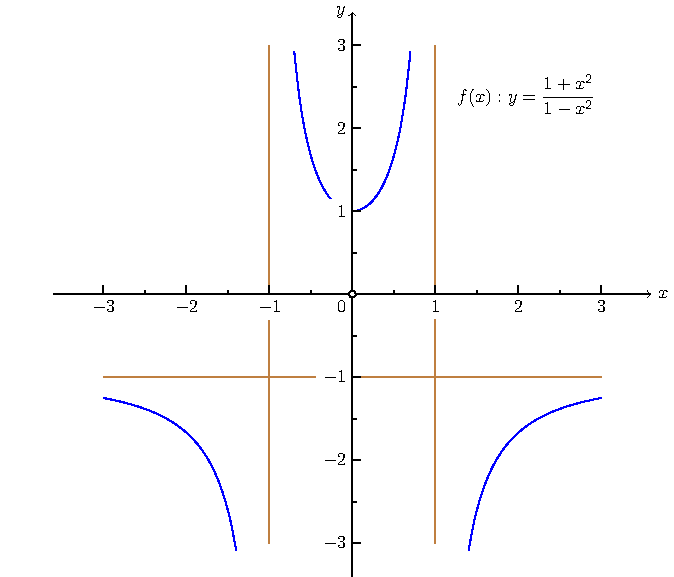
\includegraphics[width=1\linewidth]{MAI007.pdf}
    \captionof{figure}{Graf funkce $f(x):y=\dfrac{1+x^2}{1-x^2}$}
    \label{MAI:fig_007}
  \par}
\end{example}
    %-------------------------------------------------------------------

} %tikzset
%---------------------------------------------------------------------------------------------------
\printbibliography[heading=subbibliography]
\addcontentsline{toc}{section}{Seznam literatury} 
%--------------------Primitive Functions ----------------------------------------------------------
  %==================================== Primitivní funkce ======================================================
\chapter{Primitivní funkce}
\minitoc
\newpage
  %----------------------------Neurčitý integrál----------------------------------------------------
  \section{Motivace}
    Problém \emph{neurčitého integrálu}, neboli \textbf{primitivní funkce}, lze vyložit velmi jednoduše: 
    Máme podezření, že zadaná funkce \(f(x)\) vznikla derivováním jisté, zatím neznámé, funkce \(F(x)\). 
    Dokážeme ji najít? 
  
    K danému problému můžeme přistupovat také fyzikálně: Zavedením pojmu derivace funkce jsme motivovali 
    důležitým požadavkem definovat okamžitou rychlost pohybu bodu po přímce. Existuje přirozeně i požadavek 
    opačný, tj. nalézt zákon dráhy pohybu bodu po přímce, je-li dána jeho okamžitá rychlost jako funkce 
    času \cite[s.~253]{Brabec1989}. Vše si ukážeme na následujícím příkladu:  
   
    \begin{example}
      Je dána okamžitá rychlost $v$ pohybu bodu po přímce (ose) $x$ rovnicí $v(t) = 2t + 1$, $t\in\langle 
      -\infty,+\infty \rangle$. Najděte zákon dráhy pohybu, je-li známo, že v čase $t = 0$ měl bod polohu 
      $x = x_0$.
      \newline
      \textbf{řešení:}\newline
      Označíme-li $x(t)$ polohu bodu v okamžiku $t$, pak $v(t) = \frac{dx}{dt}$. Hledáme tedy funkci $x = 
      x(t)$, pro níž platí 
      \begin{align}
        \frac{dx}{dt} &= 2t + 1 \qquad x(0) = x_0.  \nonumber \\ 
        \shortintertext{Je ihned patrné, že první podmínce vyhovuje nekonečně mnoho funkcí}
        x(t)          &= t^2 + t + C,           \label{MA:int_ex_09}    \\ 
        \shortintertext{ kde $C$ je libovolná konstanta. Funkce, která splňuje i druhou podmínku 
          (říkáme ji též počáteční podmínka), najdeme z rovnice \ref{MA:int_ex_09} dosazením dané podmínky 
          $t = 0,\ x = x_0$. Dostaneme $x_0 = C$. Dosazením do \ref{MA:int_ex_09} za $C$ plyne hledaný 
          zákon dráhy}
        x(t)          &= t^2+t+x_0.                 \nonumber 
        \shortintertext{Jednoduchou zkouškou se přesvědčíme, že tato funkce splňuje obě dané podmínky a 
          zároveň vidíme, že hledaná primitivní funkce daných vlastností je jediná.}  \nonumber
      \end{align}
    \end{example}\vspace{-1cm}    
    Každé takové funkci, jejíž derivací je daná funkce, budeme říkat \emph{primitivní funkce} k dané 
    funkci. Na uvedeném příkladě je patrné, že k dané funkci může existovat nekonečně mnoho primitivních 
    funkcí. Množinu všech primitivních funkcí se často nazývá \textbf{neurčitým integrálem}. Po tomto 
    názorném uvedení do problému přejděme k přesné formulaci základních pojmů.
    
    \begin{definition} 
      Funkce $F: J\rightarrow \realset$, kde $J\subset \realset$ je interval, se nazývá primitivní funkce k 
      funkci $f$ na intervalu $J$ právě když, pro všechna $x\in J$ je $F'(x) = f(x)$ (v krajních bodech 
      intervalu $J$, pokud k němu patří, jde o derivace jednostranné).
    \end{definition}
    
    \begin{example} 
      K funkci $\sin x$ je primitivní funkcí na libovolném intervalu $J\subset(-\infty,+\infty)$ funkce 
      $-\cos x$, protože $(-\cos x)' = \sin x$. Ale též funkce $3-\cos x$ je primitivní funkcí k funkci $\sin 
      x$, protože $(3 - \cos x)' = \sin x$ pro všechna $x\in(-\infty, \infty)$.
    \end{example}
    
    Je vidět, že rozdíl dvou primitivních funkcí k téže funkci je konstanta. To není náhoda, jak potvrzuje 
    následující věta:
    
    \begin{lemma}
      \begin{enumerate}[label=\itshape\alph*\upshape)]
        \item Je-li funkce $F$ primitivní funkcí k funkci $f$ na intervalu $J$ a $c$ reálná konstanta, pak i 
              funkce $G = F + c$ je primitivní funkcí k funkci $f$ na intervalu $J$.
        \item Jsou-li funkce $F$ a $G$ primitivní funkce k funkci $f$ na intervalu $J$, pak funkce
              $F-G$ je na intervalu $J$ konstantní.
      \end{enumerate} 
      \begin{proof}
        Tvrzení a) plyne z definice protože $G'(x) = [F(x) + c] = F'(x) = f(x)$ pro všechna $x\in
        J$. Tvrzení b) je důsledkem věty \ref{MA1:lem_diff01}.
      \end{proof}
    \end{lemma}
    Neurčitost vyplývá právě z toho, že primitivní funkce není dána jednoznačně, je určena až na konstantu. 
    Značíme
    \begin{equation*}
      \boxed{F(x) = \int f(x)\dx + C}
    \end{equation*}
        
    Jak ale primitivní funkce hledat? V jednoduchých příkladech poslouží tabulka derivací, již čteme „zprava 
    doleva“. (Je dobré si ji uložit do paměti.) Tabulka však pokryje jen velmi málo případů, pouze 
    elementární funkce. Je tedy třeba najít metody, jak při hledání primitivních funkcí postupovat. Nejprve 
    však uvedeme dvě základní pravidla pro primitivní funkce, která plynou z pravidel pro derivování:
    \begin{align}
      \int[f(x)\pm g(x)]\dx &= \int[f(x)\pm g(x)]\dx + \int[f(x)\pm g(x)]\dx \label{MA1:eq_int10} \\
      \int cf(x)\dx         &= c \int f(x)\dx, \qquad \text{\(c\) je konstanta.} \label{MA1:eq_int11}
    \end{align}
  
  \section{Tabulka neurčitých integrálů}\label{MA:chap_tabINT}
    Pokud není nic uvedeno, platí vzorce pro všechna \(x\) a pro všechny hodnoty uvedených
    konstant. Místo platí pro \(x\) z intervalu \((-\infty,0),(0,+\infty)\) píšeme stručně
    \(x\neq0\) apod. Literatura: \cite[p.~396]{Rektorys1963}.
  
    \begin{flalign}
      & \int 0\dx = c                                        &         \label{MA:baseInt01}     \\
      & \int a\dx = ax+c                                     &         \label{MA:baseInt02}     \\
      & \int x^n\dx = \frac{x^{n+1}}{n+1}+c, \qquad
        \begin{cases}
          \forall x\in\realset\,                 
            \text{pro}&\,n\in\naturalset, n>0,         \\
          \forall x\in\realset-\{0\},            
            \text{pro}&\,n\in\naturalset, n<-1,        \\
          \forall x>0,\text{pro}\,n\in\realset\, 
            \text{pro}&\,n\notin\naturalset
        \end{cases}                                          &         \label{MA:baseInt03}     \\
      & \int\frac{1}{x}\dx = 
            \ln\abs{x}+c \hspace{1ex}\forall x\neq0          &         \label{MA:baseInt04}     \\
      & \int e^x \dx       = e^x+c                           &         \label{MA:baseInt05}     \\
      & \int\ln x\dx       = 
          x\ln x - x + c \hspace{1ex}\forall x>0             &         \label{MA:baseInt06}     \\
      & \int a^x \dx     =
          \frac{a^x}{\ln a}+c 
          \hspace{1ex}\forall a>0,\,a\neq1                   &         \label{MA:baseInt07}     \\
      & \int \sin x \dx  = -\cos x                           &         \label{MA:baseInt08}     \\
      & \int \cos x \dx  =  \sin x                           &         \label{MA:baseInt09}     \\
      & \int\frac{1}{\cos^2x}\dx      = 
          \tg x+c   \forall x\neq(2k+1)\pi,\,k\in\naturalset &         \label{MA:baseInt10}     \\ 
      & \int \frac{1}{\sin^2x}\dx     = 
         -\cotg x+c \forall x\neq k\pi,\,k\in\naturalset     &         \label{MA:baseInt11}     \\
      & \int\frac{1}{\sqrt{1-x^2}}\dx =  \arcsin x + c  =  -\arccos x + c 
          \hspace{1ex}\forall x\in(-1,1)\,x\in\realset       &         \label{MA:baseInt12}     \\
      & \int\cosh\dx = \sinh x + c                           &         \label{MA:baseInt13}     \\
      & \int\sinh\dx = \cosh x + c                           &         \label{MA:baseInt14}     \\
      & \int\frac{1}{1+x^2}\dx = \arctg x + c                &         \label{MA:baseInt15}     \\
      & \int \frac{1}{\sqrt{x^2 + 1}}\dx 
        = \ln(x + \sqrt{x^2+1}) + c  
        = \sinh^{-1}x + c                                    &         \label{MA:baseInt16}     \\ 
      & \int \frac{1}{\sqrt{x^2 - 1}}\dx 
        = \ln(x + \sqrt{x^2-1}) + c                   
        = \cosh^{-1}x + c \hspace{1ex}x\in(1,+\infty)        &         \label{MA:baseInt17}     \\
      & \int\frac{1}{\sqrt{x^2+a^2}}\dx 
        = \sinh^{-1} \frac{x}{a} = \ln (x+\sqrt{x^2+a^2})    &         \label{MA:baseInt18}     \\
      & \int \frac{1}{\sqrt{x^2-a^2}}\dx 
        = \cosh^{-1} \frac{x}{a} = \ln (x+\sqrt{x^2-a^2})    &         \label{MA:baseInt19}     
    \end{flalign}
    \vspace{-2.9em}
    \begin{flalign}
      & \int\frac{1}{\sqrt{x^2-1}}\dx 
        = \left\{ 
          \begin{array}{l l}
            \ln\abs{x+\sqrt{x^2-1}}+c      & \quad \text{pro \(\abs{x}>1\)}  \\
            \cosh^{-1}x+c                  & \quad \text{pro \(\abs{x}<1\)}
          \end{array} 
          \right.                                            &         \label{MA:baseInt20}     
    \end{flalign}
    \vspace{-2.9em}
    \begin{flalign}
      & \int\tan x \dx = \ln |\sec x| + c                    &         \label{MA:baseInt21}     
    \end{flalign}
    \vspace{-2.9em}
    \begin{flalign} 
      & \int\sec x \dx = \ln |\sec x + \tan x| + c           &         \label{MA:baseInt22}     
    \end{flalign}
    \vspace{-2.9em}
    \begin{flalign}
      & \int\sec^2 x \dx     = \tan x + c                    &         \label{MA:baseInt23}     
    \end{flalign}
    \vspace{-2.9em}
    \begin{flalign}
      & \int\sec x\tan x \dx = \sec x + c                    &         \label{MA:baseInt24}     \\
      & \int\frac{a}{a^2+x^2}\dx = \tan^{-1}\frac{x}{a}      &         \label{MA:baseInt25}     \\
      & \int\frac{a}{a^2-x^2}\dx = 
          \frac{1}{2}\ln\left|\frac{x+a}{x-a}\right|         &         \label{MA:baseInt26}     \\
      & \int\frac{1}{\sqrt{a^2-x^2}} \dx = 
          \sin^{-1} \frac{x}{a}                              &         \label{MA:baseInt27}     \\
      & \int\frac{a}{x\sqrt{x^2-a^2}}\dx = 
          \sec^{-1} \frac{x}{a}                              &         \label{MA:baseInt28}    
    \end{flalign}     
    
  \section{Metody určení primitivní funkce}
    Procesu hledání primitivní funkce se často říká integrování nebo integrace (od slova “integrál”), což z 
    matematického hlediska znamená provést inverzní operaci k operaci derivování. Smutnou zprávou je, že na 
    rozdíl od derivování neexistuje obecný vzorec pro integrování součinu či podílu, ani obecný vzorec pro 
    integrování složených funkcí. Při hledání integrálů složitějších funkcí se využívá např. 
    \emph{linearita, metoda per partes, substituční metoda}, popř. některé další speciální metody. Řešitel 
    v mnoha případech musí projevit důvtip a intuici, která mu pomůže nalézt primitivní funkci k dané 
    funkci.
  
    % --------------------------Integrace po částech - per partes-------------------------------------------
    \subsection{Integrace po částech - per partes}
      Metoda integrace \emph{per partes} neboli \emph{po částech} využívá vzorce pro derivaci součinu 
      funkcí. Připomeňme si jej: Pro derivaci součinu dvou funkcí \(u(x)\) a \(u(x)\) platí
      \cite[p.~137]{Musilova2009MA1}.
      \begin{align}
        [u(x)v(x)]' &= u(x)'v(x) + u(x)v'(x).  \label{MA:eq_Int29} \\
        \shortintertext{Primitivní funkcí levé strany je \(F(x) = u(x)v(x)\), a tedy}
        u(x)v(x)    &=  \int u'(x)v(x)\dx + \int u(x)v'(x)\dx \nonumber
      \end{align}  
      za předpokladu, že existují obě primitivní funkce na pravé straně. K čemu může tento samozřejmý 
      vzorec sloužit při hledání primitivní funkce? Dejme tomu, že zadaná funkce \(f(x)\), k níž máme 
      hledat funkci primitivní, je tvaru \(f(x) = u'(x)v(x)\), a my si s ní nevíme rady. Je však možné, že 
      bychom si docela dobře poradili s primitivní funkcí k funkci \(g(x) = u(x)v(x)\). A předchozí vzorec 
      umožňuje nahradit výpočet neurčitého integrálu z funkce \(f(x)\) výpočtem neurčitého integrálu z 
      funkce \(g(x)\), tedy
      \begin{equation}\label{ma:eq_perpartes}
        \int u'(x)v(x)\dx = u(x)v(x) - \int u(x)v'(x)\dx 
      \end{equation}
      \begin{example}
        Máme za úkol najít primitivní funkci k funkci \(f(x) = x\sin x\). Představíme-li si ji jako součin 
        \(f(x) = u'(x)v(x)\), kde \(u'(x) = \sin x\), tj. \(u(x) = —\cos x\), a \(v(x)= x\), tj. \(v'(x) 
        = 1\), dostaneme
        \begin{equation*}
          \int x\sin x\dx = -x\cos x + \int\cos x\dx = -x\cos x + \sin x + C.
        \end{equation*}          
      \end{example}
      Není vždy jednoduché rozpoznat, jak máme rozložit funkci \(f(x)\) na součin funkcí \(u'(x)\) a 
      \(v(x)\). Takový rozklad není určen jednoznačně a požadavek na něj bychom mohli (dosti nepřesně) 
      formulovat tak, aby funkce \(v'(x)\) byla jednodušší než v \(v(x)\) (například derivováním polynomu 
      se snižuje jeho stupeň) a funkce \(u'(x)\) a \(u(x)\) aby byly zhruba „stejně složité“ (například 
      \(u'(x) =e^x\), \(u(x) = e^x\), nebo \(u'(x) = \cos x\), \(u(x) = \sin x\), apod.). Spolehlivě 
      používat metodu per partes se však můžeme naučit pouze studiem vyřešených příkladů z literatury a 
      praktickým procvičováním \cite[p.~138]{Musilova2009MA1}.
      
      \begin{example}
        (\emph{Umělý rozklad na součin}): Někdy zadaná funkce \(f(x)\) jako součin vůbec nevypadá, a přesto 
        je použití metody per partes vhodné. Například pro elementární funkci \(f(x) = \ln x\) sice najdeme 
        primitivní funkci \ref{MA:baseInt06} v tabulce základních neurčitých integrálů z odstavce 
        \ref{MA:chap_tabINT}, ale je možné postupovat i jinak. Představme si \(f(x)\) jako součin 
        \(f(x) = 1\cdot\ln x\) a zvolme \[u'(x) = 1 ⇒ u(x) = x, \qquad v(x) = lnx ⇒ v'(x) = \frac{1}{x}\] 
        Pak \[\int \ln\dx = x\ln x - \int x\cdot\frac{1}{x}\dx = x\ln x - x.\]
      \end{example}
  
    %--------------------------- Substituční metoda ----------------------------------------------
    \subsection{Substituční metoda I}
      Tato metoda \emph{substituce} neboli \emph{náhrady} spočívá v tom, že vhodně zvolenou funkci 
      obsaženou v předpisu \(f(x)\) označíme jako novou jednoduchou proměnnou. Čeho tím dosáhneme? 
      Předpokládejme například, že \[f(x)=\varphi'(x)g[\varphi(x)]\] a označme jako novou proměnnou \(u = 
      f(x)\). Že to vypadá, jako bychom se chystali použít vzorec pro derivaci složené funkce? Správně! 
      Dejme tomu, že známe primitivní funkci \(G(u)\) k funkci \(g(u)\). Pak platí
      \begin{align*}
       \left[G\left(\varphi(x)\right)\right]' 
          &= G'\left[\varphi(x)\right]\cdot\varphi'(x) =
             g\left[\varphi(x)\right]\cdot\varphi'(x), \qquad\text{a tedy}   \\
       \int \varphi'(x) g\left[\varphi(x)\right]\dx &=  G\left[\varphi(x)\right]. 
      \end{align*}      
      Na základě těchto úvah formulujeme následující větu:
      \begin{lemma}
        Jestliže
        \begin{equation}\label{ma:eq_subst1}
          \int{f(u)du}=F(u)+C
        \end{equation}
        a $u=\varphi(x)$, pak
        \begin{equation}\label{ma:eq_subst2}
            \int{f[\varphi(x)]\varphi'(x)du}=F(\varphi(x))+C
        \end{equation}
      \end{lemma}
  
      Základem úspěchu při aplikací věty je správný výběr funkce $\varphi(x)$. Praxe je totiž
      taková, že výpočet konkrétních příkladů je schématicky veden od rov. \ref{ma:eq_subst2} ke
      vzorci rov. \ref{ma:eq_subst1}.
      
      \begin{example} Jak poznat kandidáta na substituční metodu I
        Počítejme neurčitý integrál \[\int \frac{x}{\sqrt{x^2+1}}.\]
        Vidíme, že čitatel funkce za integrálem je až na násobení konstantou derivací výrazu pod odmocninou. 
        Při označení \(u=\varphi(x) = x^2 + 1\) dostáváme \(\varphi'(x) = x\), 
        \begin{equation*}
          \int\frac{x}{\sqrt{x^2+1}}\dx = \frac{1}{2}\int\frac{2x}{\sqrt{x^2+1}}\dx
                                        = \frac{1}{2}\int\frac{1}{\sqrt{u}}\dd{u} = \sqrt{u} + C 
                                        = \sqrt{x^2 + 1} + C  
        \end{equation*}
      \end{example}
      
      \begin{example}\label{ma:ex_sub_metoda}$\displaystyle\int{e^{x^{x^2}}dx}$
        \begin{equation*}
            \int{e^{x^{x^2}}dx}=
               \left[
                 \begin{array}{c}u=x^2 \\ du=2xdx\end{array}
               \right]=
               \frac{1}{2}\int{e^udu}=\frac{1}{2}e^u=\frac{1}{2}e^{x^2}+C.
        \end{equation*}
      \end{example}
      \begin{example}$\displaystyle\int{x^3e^{x^4}}dx \qquad x\in R$
        \begin{align*}
          \displaystyle\int{x^3e^{x^4}}dx
             &= 
             \left[
               \begin{array}{cc}
                  u=x^4   & du=4x^3dx \Rightarrow \displaystyle\frac{du}{4} = x^3dx  \\
               \end{array}
             \right]                                                                           \\
             &= \frac{1}{4}\int{e^u}du = \frac{e^u}{4} = \frac{e^{x^4}}{4} + C 
        \end{align*}
      \end{example}

    % -------------------Substituční metoda II----------------------------------------------------------------
    \subsection{Substituční metoda II}
      Druhý typ substituční metody spočívá naopak v tom, že na místo původní proměnné \(x\) dosadíme vhodnou 
      funkci \(x = \psi(t)\). Místo primitivní funkce k funkci \(f(x)\) pak hledáme primitivní funkci k 
      funkci \(g(t) = f[\psi(t)]\psi'(t)\). Skutečně, je-li \(F(x)\) primitivní funkcí k \(f(x)\), pak 
      derivací složené funkce \(G(t) = F[\psi(t)]\) dostaneme
      \begin{equation*}
       G'(t) = F'[\psi(t)]\psi'(t) = f[\psi(t)]\psi'(t) = g(t).
      \end{equation*}
      \begin{example} Náhrada proměnně \(x\) funkcí
        Typické jsou neurčité integrály, které vedou na goniometrické substituce, například
        \[\int\sqrt{1-x^2}\dx\]
        
        Označme \(x=\psi(t)=\sin(t)  \Rightarrow \psi'(t)=\cos(t)\) a můžeme psát
        \begin{align*}
          \int\sqrt{1-x^2}\dx 
            &= \int\sqrt{1-\sin^2t}\cos t\dd{t} = \int\cos^2 t \dd{t} = \int\frac{1+\cos2t}{2}\dd{t}\\
          \frac{1}{2}t+\frac{\sin2t}{4}+C
            &= \frac{1}{2}\arcsin x + \frac{2\sin t\cos t}{4} 
             = \frac{1}{2}\arcsin x + \frac{x\sqrt{1-x^2}}{2} + C.
        \end{align*}
        Správně bychom měli místo \(\sqrt{1 - \sin^2x}\) psát \(\abs{\cos x}\). Vzhledem k tomu, že jde o 
        neurčitý integrál, je možné hledat primitivní funkci na intervalu, kde platí \(\cos x = \abs{\cos 
        x}\).
      \end{example}
      Jistě nám neuniklo, že princip substitučních metod I a II je stejný. Jsou totiž obě založeny na použití 
      pravidla pro derivaci složené funkce.
  
    % ---------Integrování součtu, úprava integrandu a integrování rozkladem----------------------------------
    \subsection{Integrování součtu, úprava integrandu a integrování rozkladem}
      \begin{example}
        Zdroj \cite[s.~29]{Knichal}.
        \begin{equation}\label{MA:int_ex_01}
          \int{\frac{x^4+3x^3-3x^2+3x}{x^2+1}\dx}
        \end{equation}
        Dělením čitatele integrandu jmenovatelem  dostaneme rozklad integrandu na součet funkcí,
        jejich integrály najdeme snadno:
         \begin{equation*} 
           \polylongdiv[style=C,div=:]{x^4+3x^3-3x^2+3x}{x^2+1}
         \end{equation*}
         \begin{align*}
           \shortintertext{Tedy}
           \frac{x^4+3x^3-3x^2+3x}{x^2+1}                 &= x^2+3x-4+\frac{4}{x^2+1} \\
           \intertext{Pro uvedený integrál dostaneme} 
           \int{\frac{x^4+3x^3-3x^2+3x}{x^2+1}\dx}        &=                 \\
           \int{\left(x^2+3x-4+\frac{4}{x^2+1}\right)\dx} &= 
             \frac{x^3}{3}+\frac{3x^2}{2}-4x+4\arctan x + C.
         \end{align*}
      \end{example}
      
      \begin{example}
        Zdroj \cite[s.~29]{Knichal}.
        \begin{equation}\label{MA:int_ex_03}
          \int\frac{3}{(1+x^2)x^2}\dx
        \end{equation}
        Integrand upravíme přičtením a odečtením výrazu $3x^2$ v čitateli zlomku takto:
        \begin{align*}
          \frac{3}{(1+x^2)x^2} 
            &= \frac{3+3x^2-3x^2}{(1+x^2)x^2} = \frac{3}{x^2}-\frac{3}{1+x^2}                      \\  
          \intertext{Tedy v každém otevřeném intervalu, který neobsahuje bod \(x=0\), platí}
          \int{\frac{3}{(1+x^2)x^2}\dx} 
            &= 3\int{\frac{1}{x^2}dx} - 3\int{\frac{1}{1+x^2}dx}                                   \\
            &= -\frac{3}{x}-3\arctan x + C. 
        \end{align*}
      \end{example}
      
      \begin{example}
        Zdroj \cite[s.~30]{Knichal}.
        \begin{equation}\label{MA:int_ex_04}
          \int{\sqrt{1+\cos2x}\dx}
        \end{equation}
        Funkci $\sqrt{1+\cos2x}$ upravíme na základě goniometrické identity \ref{MA1:eq_cos2x}
        \begin{align*}
          1+\cos2x       &= 1+\cos^2x-\sin^2x=2\cos^2x                                         \\
          \shortintertext{takto}
          \sqrt{1+\cos2x}&=\sqrt{2\cos^2x} = \sqrt{2}|\cos x| = \varepsilon\sqrt{2}\cos x,     \\
          \shortintertext{kde}
          \varepsilon &=
            \begin{cases} 
             +1, &  x\in \left(-\frac{\pi}{2}+2n\pi,\frac{\pi}{2}+2n\pi\right), \\
             -1, &  x\in \left(\frac{\pi}{2}+2n\pi,\frac{3\pi}{2}+2n\pi\right),
            \end{cases}                                                                        \\
          \intertext{$n$ je přirozené číslo. Proto pro $x$ ležící v uvedených intervalech je}
          \int\sqrt{1+\cos2x}\dx & = \varepsilon\sqrt{2}\int\cos x\dx 
                                   = \varepsilon\sqrt{2}\sin x + C.
        \end{align*}
      \end{example}
      
      \begin{example}
        Zdroj \cite[s.~30]{Knichal}.
        \begin{equation}\label{MA:int_ex_05}
          \int\cos^2\frac{x}{2}\dx
        \end{equation}
        Integrand upravíme na součet dvou tabulkových integrálů použitím vzorce
        \begin{align*}
          \cos^2\frac{x}{2} &= \frac{1}{2}(1+\cos x)     \\ 
          \shortintertext{takže}
          \int{\cos^2\frac{x}{2}}\dx 
                            &= \frac{1}{2}\int{(1+\cos x)}\dx = \frac{1}{2}(x+\sin x) + C.
        \end{align*}          
      \end{example}
      
      \begin{example}
        Zdroj \cite[s.~30]{Knichal}.
        \begin{equation}\label{MA:int_ex_06}
          \int{\tan^2x}\dx
        \end{equation}
        funkci napíšeme ve tvaru 
        \begin{align*}
          \tan^2x &= \frac{\sin^2x}{\cos^2x}=\frac{1-\cos^2x}{\cos^2x} = \frac{1}{\cos^2x}-1   \\
          \shortintertext{takže}
          \int{\tan^2x}dx &= \int{\left(\frac{1}{\cos^2x}-1\right)}\dx = \tan x - x + C.  
          \intertext{$\forall x\in\left(-\frac{\pi}{2}+k\pi, \frac{\pi}{2}+k\pi\right)$,
                     $k\in\naturalset$.}
        \end{align*}          
        
      \end{example}
      
      \begin{example}
        \begin{equation}\label{MA:int_ex_07} 
          \int\frac{\cos2x}{\cos^2x\cdot\sin^2x}\dx, 
            \qquad (\sin^2x\cos^2x\neq0; x\neq k\frac{\pi}{2}; k\in Z)
        \end{equation} 
       Integrand upravíme pomocí vzorce pro dvojnásobný úhel \ref{MA1:eq_cosx2}:
        \begin{equation*}
          \int\frac{\cos^2x-\sin^2x}{\cos^2x\cdot\sin^2x}\dx = 
            \int\frac{1}{\sin^2x}\dx - \int\frac{1}{\cos^2x}\dx = -\cot x - \tan x + C.
        \end{equation*}
      \end{example}
      
      \begin{example}
       \begin{equation}\label{MA:int_ex_08}
         \int\frac{1}{\cos x\cdot\sin x}\dx, 
           \qquad (\sin x\cos x\neq0; x\neq k\frac{\pi}{2}; k\in Z)
       \end{equation}
       Integrand rozšíříme o funkci $\displaystyle{\frac{1}{\cos^2x}}$
        \begin{equation*}
          \bigintss\dfrac{\dfrac{1}{\cos^2x}}{\dfrac{\sin x\cdot\cos x}{\cos^2x}} \dx = 
          \bigintss\dfrac{\dfrac{1}{\cos^2x}}{\tan x}\dx = \ln\abs{\tan x} + C.
        \end{equation*}            
      \end{example}
  
    %--------------------------- Integrace racionální funkce--------------------------------------
    \subsection{Integrace racionální funkce}
      Některé příklady v předchozím odstavci, (viz např. \ref{MA:int_ex_01} a 
      \ref{MA:int_ex_02}) jsme dělením čitatele integrandu jmenovatelem dostali rozklad
      integrandu na součet racionální funkce (polynomu) a ryze lomené racionální funkce.
      Integrování polynomu je snadné, neboť jde o součet integrálů tvaru $\int c_kx^k dx$, kde
      $k$ je celé nezáporné číslo. Omezíme se tedy na integrování \emph{ryze lomené racionální
      funkce},  tj. funkce ve tvaru $P(x)/Q(x)$, kde $P(x), Q(x)$ jsou polynomy, přičemž stupeň
      polynomu $P(x)$ je menší než stupeň polynomu $Q(x)$. Taková funkce může vzniknout součtem
      několika jednoduchých zlomků.
      
      \begin{example}
        Upravte
        \begin{align*}
          \frac{1}{x-1}+\frac{x+2}{x^2+x+3} 
            & = \frac{x^2+x+3+x^2+x-2}{(x-1)(x^2+x+3)}              \\
            & = \frac{2x^2+2x+1}{x^3+2x-3}
        \end{align*}          
      \end{example}
      
      Jsme tedy vedeni myšlenkou, zda naopak každá ryze lomená racionální funkce se dá rozložit
      na součet jednoduchých zlomků určitého tvaru - budeme jim říkat \texttt{parciální zlomky},
      které umíme integrovat. Tím se budume zabývat v dalších odstavcích. 
            
      \begin{example}
        \begin{equation}
          \int\frac{1}{x^2 - x + 1}\dx, \qquad x\in R
        \end{equation}
        Kvadratický polynom ve jmenovateli upravíme na čtverec $f(x) = (x + m)^2 + n$:
        \begin{align*}
          \int\dfrac{1}{\left(x-\dfrac{1}{2}\right)^2+\dfrac{3}{4}}\dx   &=
            \dfrac{1}{\sqrt{1-\left(\dfrac{1}{2}\right)^2}}\arctan
            \dfrac{x-\dfrac{1}{2}}{\sqrt{1-\left(\dfrac{1}{2}\right)^2}}                       \\
          \dfrac{2}{\sqrt{3}}\arctan\dfrac{2x-1}{\sqrt{3}}               &=
            \dfrac{2\sqrt{3}}{3}\arctan\dfrac{\sqrt{3}(2x-1)}{3} + C
        \end{align*}
      \end{example}     
      
      \begin{definition} Parciální (částečným) zlomkem, budeme nazývat zlomek tvaru
         \begin{equation}
            \frac{A}{(x-\alpha)^k} \qquad\text{nebo}\qquad\frac{Mx + N}{x^2 + px +q}
         \end{equation}  
         $A,\ M,\ N,\ \alpha\ , p,\ q$ reálné $p^2-4q < 0$, $k$ celé nezáporné.         
      \end{definition}
      
      Integrál prvního zlomku, tj. $\displaystyle{\int\frac{A}{(x-\alpha)^k}\dx}$, vypočteme substitucí 
      $x-\alpha=t$, odtud plyne $dx = dt$,
      \begin{equation}\label{MA:int_ex_14}
        \int\frac{A}{(x-\alpha)^k}dx = \int\frac{A}{t^k}dt.
      \end{equation}
      Tento integrál se rovná
      \begin{equation}\label{MA:int_ex_16}
        -\frac{A}{k-1}\frac{1}{(x-\alpha)^{k-1}} + C.
      \end{equation}        
      je-li $k>1$, a rovná se $A\ln|x-\alpha| + C$, je-li $k = 1$. Výsledek platí na každém
      intervalu neobsahujícím bod $\alpha$.
      
       U integrál druhého zlomku uvedeme postup výpočtu pro $k = 1$. 
      \begin{align*}
         \intertext{\(\displaystyle\int{\frac{Mx + N}{x^2+px+q}dx}\)}
           \qquad &=  \int{\frac{Mx}{x^2+px+q}dx} + \int{\frac{N}{x^2+px+q}dx}                     \\  
           \qquad &=  \frac{M}{2}\int{\frac{(2x + p) - p}{x^2+px+q}dx} + 
                     N\int{\frac{1}{x^2+px+q}dx}                                                   \\ 
           \qquad &=  \frac{M}{2}\int{\frac{2x + p}{x^2+px+q}dx} + 
                      \left(N-\frac{Mp}{2}\right)\int{\frac{1}{x^2+px+q}dx.}                   
      \end{align*}  
      
      Z naznačeného postupu je vidět hlavní myšlenka: upravit integrál na lineární kombinaci dvou integrálů, 
      z nichž první má v čitateli integrandu derivaci jmenovatele a je podle příkladu *** roven 
      $\ln|x^2+px+q|$ kde $x^2+px+q >0$ pro $x\in R$ a integrand druhého integrálu má čitatel konstantní.
      
      Výpočet druhého integrálu probíhá takto: 
      \begin{equation}\label{MA:int_ex_10}
        \int\dfrac{1}{x^2+px+q}\dx = 
          \int\dfrac{1}{\left(x+\dfrac{p}{2}\right)^2 + q - \dfrac{p^2}{4}}\dx;
      \end{equation}
      substitucí $x+\dfrac{p}{2} = t\sqrt{q - \dfrac{p^2}{4}}$ dostáváme dále
      \begin{equation*}\label{MA:int_ex_11}
        \bigints{\frac{1}{\displaystyle{\left(x+\frac{p}{2}\right)^2 + q - \frac{p^2}{4}}}}dx 
          =\displaystyle{
            \bigints{
              \frac{\sqrt{q-\frac{p^2}{4}}}{\left(q-\frac{p^2}{4}\right)(t^2+1)}}dt
            }   
      \end{equation*}
      po úpravě dostaneme tabulkový integrál
      \begin{equation}\label{MA:int_ex_12}
        \frac{1}{\sqrt{q-\frac{p^2}{4}}}\int{\frac{dt}{t^2+1}},
      \end{equation}
      jehož řešení je  
      \begin{equation*}\label{MA:int_ex_13}
        \frac{1}{\sqrt{q-\frac{p^2}{4}}}\arctan{t} 
          = \sqrt{q-\frac{p^2}{4}}\arctan\frac{x+\frac{p}{2}}{\sqrt{q-\frac{p^2}{4}}}.     
      \end{equation*}   
      Z postupu je opět vidět hlavní myšlenka: úprava integrandu na tvar $\dfrac{1}{t^2+1}$.
      Jmenovatel $x^2+px+q$ jsme doplnili na úplný čtverec a užili uvedenou substituci (uvažme,
      že $q-\dfrac{p^2}{4}>0$, protože diskriminant $\dfrac{p^2}{4}-q$ trojčlenu $x^2+px+q$ je
      podle předpokladu záporný). Výsledek platí u obou integrálu v intervalu \((-\infty,
      +\infty)\).
      
      % -----------------------Funkce typu {f(x)=\sqrt{ax+b}} ------------------------------------
      \subsubsection*{Funkce typu $\boxed{f(x)=\sqrt{ax+b}}$ :}
         Funkci, jež je dána rovnicí, jež obsahuje polynomy proměnné x  ve výrazu $\sqrt{ax+b}$,
         v němž $ax+b>0$, $a>0$, integrujeme pomocí substituce:
         \begin{equation}\label{ma:eq_sub_fce1}
             u=\sqrt{ax+b},\quad du=\frac{1}{2}\frac{a}{u}dx,\quad dx=2\frac{u}{a}du
         \end{equation}
         Je-li potřeba dosadit do integrované funkce také za $x$, vyjádříme ze substituční
         rovnice $x=\frac{u^2-b}{a}$.
      % ----------------------Funkce typuf(x)=\frac{1}{\sqrt{x^2+a}}, a\neq0 -------------------- 
      \subsubsection*{Funkce typu $\boxed{f(x)=\frac{1}{\sqrt{x^2+a}}}, a\neq0$ :}
         \begin{example}\label{ma:ex_sub_metoda1}$\displaystyle\int{\frac{1}{\sqrt{x^2+a}}dx}$:\vskip0.5mm
           \textbf{Řešení}: Užijeme \textbf{Eulerovu substituci}\vskip1mm 
                            \hskip17mm$u=x+\sqrt{x^2+a},\quad \displaystyle{du=\frac{u}{\sqrt{x^2+a}}dx}$,
                            $\displaystyle{\frac{du}{u}=\frac{dx}{\sqrt{x^2+a}}}.$
           \begin{equation*}
            \int{\frac{1}{\sqrt{x^2+a}}dx}=\int{\frac{du}{u}}=\ln|u|=\ln|x+\sqrt{x^2+a}|+C
           \end{equation*}
         \end{example}
  
    % --------------------------Integrály goniometrických funkcí----------------------------------     
    \subsubsection{Integrace goniometrických funkcí}
      
    % ---------------- Rozklad ryze lomené funkce v parciální zlomky -----------------------------------------
    \subsubsection{Rozklad ryze lomené funkce v parciální zlomky}
      Nechť je dána racionální funkce $R = \frac{P}{Q}$ s reálnými koeficienty. Můžeme
      předpokládat, že je \emph{ryze lomenná}\footnote{tj. stupeň polynomu $P$ je menší než
      stupeň polynomu $Q$}. Pokud by tomu tak nebylo, dostaneme dělením čitetele jmenovatelem
      zlomku součet polynomu a ryze lomené racionální funkce.
      
      \begin{example}$\displaystyle\int{\frac{8x-31}{x^2-9x+14}}dx$\cite[s.~90]{Knichal}\newline
        Kořeny polynomu ve jmenovateli $\alpha_1 = 2$, $\alpha_2 = 7$ jsou jednoduché - každému z
        nich bude v rozkladu odpovídat jen jeden člen $$\frac{8x-31}{x^2-9x+14} = \frac{A}{x-2}
        + \frac{B}{x-7}.$$ Členy mnohočlenu na pravé straně seřadíme podle mocnin $x$ $$8x-31 =
         x(A+B)+(7A-2B).$$ Porovnáním odpovídajících si koeficientů dostaneme
        \begin{align*}
          8   &=   \; A + \, B \\
          -31 &= -7A - 2B
        \end{align*}
        Řešením této soustavy je $A = 3, B = 5$. Platí tedy (pro všechna $x \neq 2$ a $x \neq 7$)
        $$\frac{8x-31}{x^2-9x+14} = \frac{3}{x-2} + \frac{5}{x-7}.$$
        \begin{align*}
          \int{\frac{8x-31}{x^2-9x+14}}dx 
            &= \int{\frac{3}{x-2}}dx + \int{\frac{5}{x-7}}dx      \\
            &= 3\ln|x-2| + 3\ln|x-7| + C.
        \end{align*}
        Výsledek platí v každém intervalu, který neobsahuje body $x = 2$,$x = 7$.
      \end{example}
      
      \begin{example}\label{MA:eq_ex1}$\displaystyle\int{\frac{19x+15}{x^2-x-2}}dx \qquad x\in
        R-\{1,2\} $ \newline Kořeny polynomu ve jmenovateli $\alpha_1 = -1$, $\alpha_2 = 2$ jsou
        jednoduché - každému z nich bude v rozkladu odpovídat jen jeden člen: 
        \begin{align*}
          \frac{19x+15}{x^2-x-2}     &= \frac{A}{x+1} + \frac{B}{x-2} \\
                           19x +15   &= A(x-2) + B(x+1)               \\
                           19x +15   &= x(A+B) - 2A + B               \\
                           19        &= A + B                         \\
                                15   &=        - 2A + B
        \end{align*}              
        Řešením této soustavy je $A = \frac{4}{3}$, $B = \frac{53}{3}$.
        \begin{equation*}
          = \frac{4}{3}\int{\frac{1}{x+1}}dx+\frac{53}{3}\int{\frac{1}{x-2}}dx 
          = \frac{4}{3}\ln|x+1| - \frac{53}{3}\ln|x-2| +  C
        \end{equation*}      
      \end{example}
  
      \begin{example}
        $\displaystyle\int{\frac{2x^2+34x+14}{x^3-4x^2-x-4}}dx$\cite[s.~90]{Knichal}\newline
        Polynom $Q(x)=x^3-4x^2-x-4$ má kořeny $\alpha_{1,2}=\pm1$, $\alpha_{3}=-4$, které jsou
        jednoduché tj. $Q(x)=(x-1)(x+1)(x+4)$ $$\frac{2x^2+34x+14}{x^3-4x^2-x-4} =
        \frac{A}{x-1}+\frac{B}{x+1}+\frac{C}{x+4}$$ Vynásobíme-li tuto rovnici společným
        jmenovatelem zlomků pravé strany (polynomem $Q(x)$), dostaneme
        \begin{align*}
          2x^2+34x+14 &= A(x+1)(x+4)+B(x-1)(x+4)+C(x-1)(x+1) \\
          \intertext{čili}
          2x^2+34x+14 &= A(x^2+5x+4)+B(x^2+3x-4)+C(x^2-1) \\
          2x^2+34x+14 &= (A+B+C)x^2+(5A+3B)x + (4A-4B-C)
        \end{align*}
        Porovnáním odpovídajících si koeficientů u stejných mocnin $x$  dostaneme pro nez\-ná\-mé
        koeficienty $A, B, C$ soustavu rovnic
        \begin{align*}
        % \nonumber to remove numbering (before each equation)
           A+   B + C &= 2 \\
          5A + 3B     &= 34 \\
          4A - 4B - C &= 14
        \end{align*}
        Řešením této soustavy je $A = 5, B = 3, C = -6$ a tedy
        $$\frac{2x^2+34x+14}{x^3-4x^2-x-4} = \frac{5}{x-1}+\frac{3}{x+1}-\frac{6}{x+4}$$
        \begin{align*}
          \int{\frac{2x^2+34x+14}{x^3-4x^2-x-4}}dx 
            &= \int{\frac{5}{x-1}}dx + \int{\frac{3}{x+1}}dx + \int{\frac{6}{x+4}}dx            \\
            &= 5\ln|x-1| +  3\ln|x+1| - 6\ln|x+4| +C.
        \end{align*}
      \end{example}
  
      \begin{example}$\displaystyle{\int\frac{2x+3}{2x^3+2}dx} \qquad x\in R-{-1}$\newline
        a
      \end{example}

  % ---------------- Sbírka řešených příkladů ----------------------------------------------------------------
  \newpage
  \section{Sbírka řešených příkladů}
    Hledej primitivní funkce \(F(x)\) k následujícím funkcím
    
  \begin{example}\(\displaystyle\int{xe^x\dx}\)
    \begin{equation*}
        \int{xe^xdx}=
          \left[\begin{array}{cc}
            u=x   & dv=e^x \\
            du=dx & v=e^x
          \end{array}\right]=
          xe^x-\int{e^x\dx} = xe^x - e^x+C
    \end{equation*}
  \end{example}
  
  \begin{example}$\displaystyle\int{\arctan xdx} \qquad x\in R$
    \begin{align*}
       \int{\arctan xdx}                      &= 
         \left[\begin{array}{cc} 
                  u =\arctan x                     &  dv= 1  \\ 
                 du =\displaystyle\frac{1}{x^2+1}  &   v= x
               \end{array}
         \right]  =                                                                  \\
       x\arctan x-\int\frac{x}{x^2+1}         &= 
         \left[\begin{array}{c} 
                  x^2 + 1 = t  \Rightarrow 2xdx = dt        \\ 
                      xdx = \displaystyle{\frac{dt}{2}}
               \end{array} 
         \right] =                                                                   \\ 
       x\arctan x-\frac{1}{2}\int\frac{dt}{t} &= x\arctan x-\frac{1}{2}\ln|t|        \\
         &=   x\arctan x-\frac{1}{2}\ln|1+x^2|+C                                     \\
    \end{align*}
  \end{example}
  
  \begin{example}$\displaystyle\int{\sqrt{x^2+a}dx}$, kde $a\neq0, x^2+a>0$
    \begin{align*}
      \int{\sqrt{x^2+a}\dx}                           &=
        \left[
          \begin{array}{cc} 
             u =\sqrt{x^2+a}              & dv = 1 \\ 
            du =\displaystyle
                  \frac{x}{\sqrt{x^2+a}}  &  v = x
          \end{array}
        \right]                                                                                   \\
      x\sqrt{x^2+a}-\int{\frac{x^2}{\sqrt{x^2+a}}\dx} &= 
        \displaystyle{x\sqrt{x^2+a}-\int{\frac{x^2+a-a}{\sqrt{x^2+a}}\dx}}                        \\
      \int{\sqrt{x^2+a}\dx}                           &= 
        \displaystyle{x\sqrt{x^2+a}-\int{\sqrt{x^2+a}\dx} + \int{\frac{a}{\sqrt{x^2+a}}\dx}}      \\
      \int{\sqrt{x^2+a}\dx}                           &= 
        \frac{1}{2}\left[x\sqrt{x^2+a}+a\int{\frac{1}{\sqrt{x^2+a}}}\dx\right]
    \end{align*}
    Integrál na pravé straně vyjádříme podle příkladu \ref{ma:ex_sub_metoda1}
    $\displaystyle{\int{\frac{1}{\sqrt{x^2+a}}\dx}}$ a výsledek do\-sta\-ne\-me ve tvaru
    $$\int\displaystyle{{\sqrt{x^2+a}\dx}=\frac{1}{2}\left[x\sqrt{x^2+a}+a\ln{|x +
    \sqrt{x^2+a}|}\right]}$$
  \end{example}
  
  \begin{example}
    \begin{equation}\label{MA:int_ex_02}
      \int{\frac{2x^4-5x^2+14x+13}{x^2-x-2}\dx} \qquad x\in R - \{1,2\}
    \end{equation}
    Dělením čitatele integrandu jmenovatelem dostaneme rozklad integrandu na součet funkcí, jejich integrály 
    najdeme snadno:
    \begin{widetext}
      \begin{equation*}
        \polylongdiv[style=C,div=:]{2x^4-5x^2+14x+13}{x^2-x-2}
      \end{equation*}
    \end{widetext}
    Zbytek po dělení představuje integrál, jež je počítán v příkladu \ref{MA:eq_ex1} a proto ho vynecháme.
    \begin{align*}
       &= 2\int x^2\dx + 2\int x\dx + \int\dx + \int\frac{19x+15}{x^2-x-2}\dx     \\
       &= \frac{2}{3}x^3 + x^2 + x + \frac{4}{3}\ln|x+1| - \frac{53}{3}\ln|x-2| + C 
    \end{align*}                
  \end{example}
    
  \printbibliography[heading=subbibliography]
  \addcontentsline{toc}{section}{Seznam literatury}
%--------------------an Integrals of functions of one real variable -------------------------------
  %====================================================================================================
% --------------------------------------------- Definite Integral -----------------------------------
\chapter{Určitý integrál}
\minitoc
\newpage  
\section{Motivace} 
  %----------------------------------
  % image: MAI_animated_integral.tex label: \label{MAI:fig_anim_int}
    % \documentclass{book}
% \usepackage{ifthen}
% \usepackage{tikz}
%   \usetikzlibrary{intersections}
%   \usetikzlibrary{calc}
% \usepackage{animate}

\newcounter{r}
\newcommand{\escalar}[1]{
\setcounter{r}{#1 * #1 * #1}
}
%
\newcounter{m}
\setcounter{m}{0}
\newcounter{mc}

% \begin{document}
    %\begin{frame}[fragile]{Animated Integral}
      %\centering
      \protect  % JAFA příkaz protect pomohl -> nemusí být \begin{frame}, který funguje divně (vysází se obsah
                % závorek, tj. [fragile]{Animated Integral})
        \begin{animateinline}[loop, poster = first, controls, palindrome]{2}
          \whiledo{\them < 21}{
            \begin{tikzpicture}[scale=1.25]
              \draw[red,thick,<->] (-1,1) parabola bend (0,0) (2.1,4.41)
                  node[below right] {$y=x^2$};
              \draw[loosely dotted] (-1,0) grid (4,4);
              %\path[use as bounding box] (-2,-1) rectangle (5,5);
              \draw[->] (-0.2,0) -- (4.25,0) node[right] {$x$};
              \draw[->] (0,-0.25) -- (0,4.25) node[above] {$y$};
              \foreach \x/\xtext in {1/1, 2/2, 3/3}
                \draw[shift={(\x,0)}] (0pt,2pt) -- (0pt,-2pt) node[below] {$\xtext$};
              \foreach \y/\ytext in {1/1, 2/2, 3/3, 4/4}
                \draw[shift={(0,\y)}] (2pt,0pt) -- (-2pt,0pt) node[left] {$\ytext$};
              %
              \setcounter{mc}{\value{m}*\value{m}}
              \shade[top color=blue,bottom color=gray!50]
                  (0,0) parabola (0.1*\them,0.01*\themc) |- (0,0);
              \escalar{\them}
              \draw (3cm,2pt) node[above]
                {$\displaystyle\int\limits_0^{\them/10}\!\!x^2\mathrm{d}x=\displaystyle\frac{\ther}{3000}$};
              \draw[fill=orange,color=orange] (0.1*\them,0.01*\themc) circle (0.5pt);
            \end{tikzpicture}
            %
            \stepcounter{m}
            \ifthenelse{\them < 21}{
                    \newframe
            }{
                \end{animateinline}\relax % BREAK
            }
          } % END \whiledo...
      \label{MAI:fig_anim_int}
    %\end{frame} 
  
% \end{document}  
  %---------------------------------- 

\subsection{Výpočet integrálu}
    \begin{example}Metodou per partes spočítejte integrály:$\displaystyle\int_1^{ln5}{(x+1)e^xdx}$
      \begin{align*}
        \int{(x+1)e^xdx} &= \int{e^xdx}+\int{x\cdot e^xdx} \\
                         &= e^x + (x-1)e^x = xe^x \\
        \int_1^{ln5}{(x+1)e^xdx} &= [xe^x]_1^{ln5} = 5ln5-e\\
      \end{align*}
      kde integrál
      \begin{equation*}
          \int{xe^xdx}=
            \left[\begin{array}{cc}
              u=x   & dv=e^x \\
              du=dx & v=e^x
            \end{array}\right]=
            xe^x-\int{e^xdx} = xe^x - e^x+C
      \end{equation*}
    \end{example}

\newpage
\section{Vlastnosti určitého integrálu}
  V této kapitole mluvíme o spojitých funkcích $\Rightarrow$ příslušné integrály tedy vždy
  existují. Čerpáno z knih:
  \cite{Knichal}.

  \begin{lemma}
    \textbf{První věta o střední hodnotě integrálního počtu}: Je-li funkce $f(x)$ spojitá v
    intervalu $\langle a, b\rangle$, existuje alespoň jeden takový bod $c\in(a, b)$, že platí

    \begin{equation}\label{MA:eq_av1}
      \int_a^b f(x)dx = (b-a)f(c).
    \end{equation}
  \end{lemma}

  \begin{proof} Použitím Lagrangeovy věty napsané pro funkci $F(x)$, primitivní na intervalu
    $\langle a, b\rangle$ k dané funkci $f(x)$. Podmínky věty jsou zřejmě splněny: $F(x)$ je
    spojitá na intervalu $\langle a, b\rangle$ a má všude derivaci $F'(x)= f(x)$. Tedy existuje
    alespoň jeden bod $c\in(a, b)$,
    
      %----------------------------------
        % image: MAI_rolle_02.tex label: \label{MA:fig_rolle_02} 
        % \documentclass{article}
% \usepackage{tikz}
% \usetikzlibrary{decorations.markings}
% \usetikzlibrary{intersections}
% \usepackage{wrapfig}                   % Floats, Figures and Captions  
% \usetikzlibrary{calc}

% \begin{document}
 
    \begin{figure}[hb!]
        \centering
        \begin{tikzpicture}
           [scale=3,line cap=round,
            % Styles
              axes/.style=,
              important line/.style={very thick},
              information text/.style={rounded corners,fill=red!10,inner sep=1ex}]
          \begin{scope}[axes]     
            \draw[->] (-0.2, 0) -- (1.5, 0) node[right] {$x$} coordinate(x axis);
            \draw[->] (0, -0.2) -- (0, 1.5) node[left] {$y$} coordinate(y axis);
          \end{scope}
          % my function  
           \draw[very thick,red](1.5,1.4) node[left=1pt,fill=white]{$y=f(x)$};
           \coordinate [label={[blue]left:$D$}] (D) at (0.3,0.5);
           \coordinate [label={[blue]right:$C$}] (C) at (1.2,1.2);
           \draw[name path=func] (D) .. controls (1.0,0.5) and (0.5,1.2) .. (C);
          % horizontal line
           \draw[name path=my_line, gray, dotted] (0.75,0) node[below, red]{$c$} -- (0.75,0.9);
          % intersection between vertical line and my function
           \fill[red, opacity=0.5, name intersections={of=func and my_line, by={intersect}}]
                (intersect) circle (1pt);
          % x-axis labels
           \draw[gray, dotted, text = blue] (D) -- +(0,-0.5) 
              node [label={[xshift=-0.2cm, yshift=0.5mm]$A$},below] (A) {$a$};
           \draw[gray, dotted, text=blue] (C) -- +(0,-1.2)
              node [label={[xshift=0.2cm, yshift=0.5mm]$B$},below] (B) {$b$};
           \draw[red](-0.05,-0.08) node[left=1pt,fill=white]{$0$};
          % y-axis labels
           \draw[gray, dotted] let \p1=(D), \p2=(intersect), \p3=(C) in (\x1,\y2)
              -- +(-\x1,0) node[left, red]{$f(c)$} 
              -- (\x1,\y2) node[above, blue] (F) {$F$} 
              -- (\x3,\y2) node[right, blue]{$E$}; 
          % dotted line between F and D
           \draw[gray, dotted] (F) -- (D);
        \end{tikzpicture}
        \caption{ }\label{MAI:fig_rolle_02}
    \end{figure}
  
%\end{document}  
      %----------------------------------   
    
      že $$F(b)-F(a) = (b-a)F'(c),$$ čímž je věta dokázána, neboť $F(b)-F(a) = \int_a^bf(x)dx$ a
      $F'(c) = f(c)$. Funkční hodnotu $f(c)$, danou podle (\ref{MA:eq_av1}) rovnicí  
      \begin{equation}\label{MA:eq_av2}
         f(c) = \frac{1}{b-a}\int_a^b f(x)dx
      \end{equation}
      nazýváme \texttt{střední hodnotou}.
  \end{proof}

  Pro spojitou nezápornou funkci $f(x)$, lze větu o střední hodnotě jednoduše geometricky
  interpretovat dle (obr.\ref{MAI:fig_rolle_02}). Levá strana (\ref{MA:eq_av1}) určuje obsah
  křivočarého lichoběžníka $ABCD$, pravá strana obsah obdélníka $ABEF$. Podle této věty nabývá
  funkce $f(x)$ aspoň v jednom bodě intervalu $(a, b)$ takové hodnoty $f(c)$, že uvažovaný
  křivočarý lichoběžník má stejný obsah jako obdélník o základně $b-a$ a výšce $f(c)$ (str. 155
  knihy \cite{Knichal}).

  \begin{example} Určete střední hodnotu $i_s$ střídavého proudu $$i(t) = I_0\sin\omega t$$ v
    časovém intervalu $\langle 0, \frac{T}{2}\rangle$ (v průběhu jedné poloviny periody). $I_0$ je
    maximální hodnota proudu (obr. \ref{MA:fig_Iav_exam}), perioda $T$ je dána vztahem $T =
    \frac{2\pi}{\omega}$
    %----------------------------------
      % image: MAI_rolle_02.tex label: \label{MA:fig_Iav_exam}
      % \documentclass{article}
% \usepackage{tikz}
% \usetikzlibrary{decorations.markings}
% \usetikzlibrary{intersections}
% \usetikzlibrary{calc}

% \begin{document}
 
      {\centering
       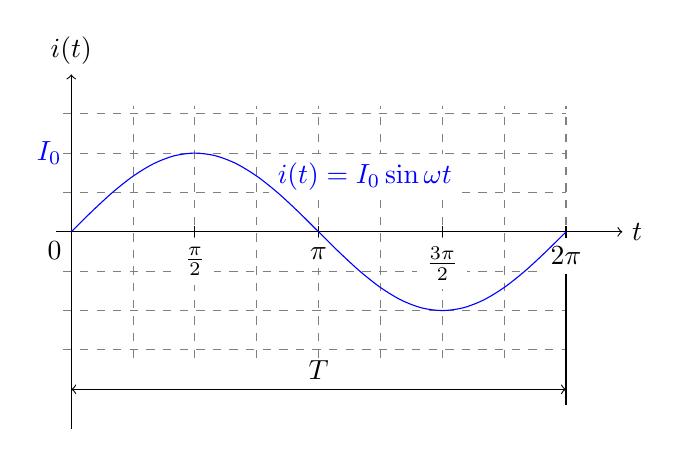
\begin{tikzpicture}[domain=0:2*pi] 
         \draw[xstep=pi/4, ystep=0.5, dashed, color=gray] (-0.1,-1.6) grid (2*pi,1.6); 
         \draw[->] (-0.2,0) -- (7,0) node[right] {$t$}; 
         \draw[->] (0,-2.5) -- (0,2) node[above] {$i(t)$}; 
         % text 
         \node[below left](0,0){$0$};
         \node[left, color=blue] at (0,1.0) {$I_0$}; 
         % period
         \draw[<->] (0,-2) -- (pi,-2) node[above]{$T$} --(2*pi,-2);
         \draw (2*pi,-2.2) -- (2*pi,0); 
         \foreach \x/\xtext in {0.5*pi/\frac{\pi}{2} ,pi/\pi, 1.5*pi/\frac{3\pi}{2}, 2*pi/2\pi}
         \draw[shift={(\x,0)}] (0pt,2pt) -- (0pt,-2pt) node[below, fill=white] {$\xtext$};  
         \node[below right, color=blue, fill=white] at (2.5,1.0) {$i(t) = I_0\sin\omega t$};
         % function 
         \draw[color=blue, smooth]   plot (\x,{sin(\x r)}); 
       \end{tikzpicture}  
       \captionsetup{type=figure}   
       \captionof{figure}{}\label{MA:fig_Iav_exam}
    \par}
  
%\end{document}  
    %----------------------------------

    Podle \ref{MA:eq_av2} bude
    \begin{align*}
     i_s &=  \frac{2}{T}
             \int_0^{\frac{T}{2}}I_0\sin\omega t\dd{t} =
             \frac{2I_0}{T}\left[-\frac{\cos\omega t}{\omega}\right]_0^{\frac{T}{2}}        \\
         &=  \frac{2I_0}{T}\frac{1}{\omega}\left(-\cos\frac{\omega T}{2}+ \cos 0\right)     \\
         &=  \frac{2I_0}{2\pi}(-\cos\pi + \cos 0) = \frac{2}{\pi}I_0 \doteq 0,637 I_0.
  \end{align*}

  Tato hodnota se rovná intenzitě elektrického proudu, při kterém by vodičem v průběhu uvažované
  poloviny periody prošel stejný elektrický náboj jako při proudu střídavém.
  \end{example}

  \begin{example} Efektivní hodnota $i_{ef}$ střídavého proudu $$i(t) = I_0\sin\omega t$$ (viz
    předchozí příklad) je definována jako odmocnina ze střední hodnoty funkce $i^2(t)$ v průběhu
    jedné periody $T = \frac{2\pi}{\omega}$. Tedy
    \begin{align*}
      i_{ef}^2 &= \frac{1}{T}\int_0^T I_0^2\sin^2\omega t\dd{t} = 
                  \frac{1}{T}\int_0^T \frac{I_0^2}{2}(1- \cos2\omega t)\dd{t}           \\
               &= \frac{I_0^2}{2T}
                  \left[
                    t-\frac{\sin2\omega t}{2\omega}
                  \right]_0^T = \frac{I_0^2}{2}
    \end{align*}
    neboť $\sin2\omega T=\sin4\pi = 0.$ Odtud $$i_{ef} = \frac{I_0}{\sqrt{2}}.$$ Střídavý proud
    $i(t) = I_0\sin\omega t$ má na témže odporu stejný výkon jako stejnosměrný proud o intenzitě
    $i = 0,707I_0$.
  \end{example}
  Následující věta může být využita k odhadu některých integrálů
  \begin{lemma}
    \textbf{Druhá věta o střední hodnotě integrálního počtu}: Jsou-li funkce $f(x)$ a $g(x)$
    spojité v intervalu $\langle a, b \rangle$ a je-li funkce $g(x)$ v $\langle a, b \rangle$
    nezáporná a nerostoucí, existuje alespoň jeden bod $c\in\langle a, b \rangle$ tak, že platí
    \begin{equation}\label{MA_eq_av3}
        \int_a^b f(x)g(x) = g(a)\int_a^c f(x)dx.
    \end{equation}
  \end{lemma}
  Zcela obdobnou větu lze vyslovit pro případ, že $g(x)$ je v intervalu $\langle a, b \rangle$
  nezáporná a neklesající, tj. na pravé straně \ref{MA_eq_av3} je pak integrál $g(b)\int_c^b
  f(x)dx$

  \begin{example} Odhadněte hodnotu integrálu
    \begin{equation}\label{MA_eq_sinx_x}
        \int_{100\pi}^{1000\pi}\frac{\sin x}{x}dx
    \end{equation}
    Řešení: Funkce $f(x) = \sin x$ a $g(x) = \frac{1}{x}$ jsou v uvažovaném intervalu $\langle
    100\pi, 1000\pi \rangle$ spojité a funkce $g(x)$ je kladná a nerostoucí.
    \begin{equation*}
      \int_{100\pi}^{1000\pi}\frac{\sin x}{x}dx = 
      \frac{1}{100\pi}\int_{100\pi}^c\sin xdx =\frac{1}{100\pi}\left(\cos100\pi - \cos c\right)
    \end{equation*}
    kde $c$ je kladné číslo z intervalu $\langle 100\pi, 1000\pi \rangle$. Dále pro všechna
    $c\in\langle 100\pi, 1000\pi \rangle$ platí $0\leq1-\cos c\leq2$, takže
    \begin{equation*}
        0\leq\int_{100\pi}^{1000\pi}\frac{\sin x}{x}dx\leq \frac{1}{50\pi}.
    \end{equation*}
  \end{example}   
%---------------------------------------------------------------------------------------------------
\printbibliography[heading=subbibliography]
\addcontentsline{toc}{section}{Seznam literatury}
%---------------------Řady-------------------------------------------------------------------------
%  \input{../src/MAI/chapters/Series.tex}
%---------------------Obyčejné diferenciální rovnice ----------------------------------------------
  % !TeX spellcheck = cs_CZ
{\tikzset{external/prefix={tikz/MAI/}}
 \tikzset{external/figure name/.add={ch09_}{}}
%---------------------------------------------------------------------------------------------------
% file ODR.tex
%---------------------------------------------------------------------------------------------------
\chapter{Obyčejné diferenciální rovnice}
\minitoc
%================Kapitola: Diferenciální rovnice 1. řádu ===========================================
  \section{Diferenciální rovnice 1. řádu}
    Řada fyzikálních principů má tvar výroku, resp. vztahu mezi jistými veličinami (funkcemi) a
    jejich změnami, vztaženými ke zvoleným nezávisle proměnným pa\-ra\-me\-trům (čas, souřadnice).
    Změny (okamžité, lokální) se nejlépe vystihují pomocí derivací. Takový zákon má pak charakter
    vztahu mezi uvažovanými veličinami a jejich derivacemi. Nejčastěji bývá vztah vyjádřen formou
    rovnosti:
    \begin{itemize}
   	  \item Newtonůw zákon: okamžitá změna hybnosti $p(t) = m(t)\cdot v(t)$ pohybujícího se
         	objektu je úměrná působící síle $F(t)$ v každém okamžiku $t$ zvoleného časového rozmezí
        	$$\frac{d}{dt}\left(m(t)\cdot v(t)\right) = F(t)\quad t\in\langle\alpha, \beta\rangle$$
      \item Kirchhoffův zákon pro LR – obvod: v okamžiku $t$ je součet napětí na cívce s indukčnosti
            $L$ a na rezistoru o odporu $R$ roven napětí $U(t)$ na svorkách zdroje. Tuto rovnost pak
            zapisujeme ve tvaru (pro L,R = konst)
            \begin{equation}
              L\frac{di(t)}{dt}+Ri=u(t), 
            \end{equation}
            kde $i=i(t)\ldots$ funkce popisující závislost proudu na čase.
    \end{itemize}
    
    Chceme-li určit funkci $i=i(t)$ popisující průběh proudu v obvodu tak, aby byl splněn příslušný
    K.z. a současně, aby byl splněn požadavek na počáteční stav:
    \begin{equation}
        L\frac{di(t)}{dt}+Ri(t)=U,\quad i(0)=I_0,\quad t\in\langle 0,+\infty)
    \end{equation}
    Metodami uvedenými později stanovíme právě jednu funkci $i=i(t)$, která je řešením dané tzv.
    \textbf{počáteční úlohy}.
    \begin{equation}
      \begin{array}{c}
         i(t)=I_0\left(1-e^{-\frac{R}{L}t}\right),\quad t\in\langle 0,+\infty), \\
         lim_{t\rightarrow +\infty}i(t)=\frac{U_0}{R},\quad lim_{t\rightarrow +0}i(t)=I_0=i(0)
      \end{array}
    \end{equation}
    \begin{itemize}
      \item tedy obvykle formulujeme úlohu najít jistou funkci tak, aby zákon byl splněn tj.
            Kirchhoffův zákon užijeme k tomu, abychom nalezli funkci $i(t)$
      \item užijeme-li rovnosti vyjadřující takový zákon k tomu, abychom určili funkci, která v
            takovém vztahu vystupuje spolu s derivacemi, stává se tento požadavek úlohou, která má
            charakter rovnice s derivacemi, neboli diferenciální rovnice. Funkce, která požadavek
            splňuje, se pak nazývá řešení diferenciální rovnice.
    \end{itemize}
    
    \begin{figure}
      \centering
      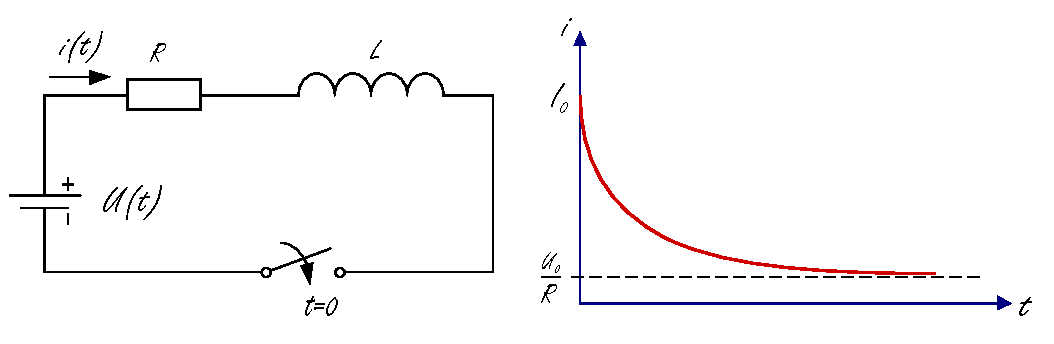
\includegraphics[width=\linewidth]{motivace.pdf}
      \caption{Graf průběhu proudu $i(t)$ po sepnutí spínače v době $t=0$.}
      \label{figure:odr_motivace}
    \end{figure}

} %tikzset
%---------------------------------------------------------------------------------------------------
%\printbibliography[heading=subbibliography]
\addcontentsline{toc}{section}{Seznam literatury}
%---------------------Numerické metody ------------------------------------------------------------
  % !TeX spellcheck = cs_CZ
{\tikzset{external/prefix={tikz/MAI/}}
 \tikzset{external/figure name/.add={ch10_}{}}
%---------------------------------------------------------------------------------------------------
% file ppst.tex
%---------------------------------------------------------------------------------------------------
\chapter{Počet Pravděpodobnosti}
\minitoc
  Slovo pravděpodobnost používáme velmi často. Jaký však je jeho přesný význam? Jsme přesvědčeni, 
  že pravděpodobnost výhry ve sportce je velmi malá. Ani pravděpodobnost, že se vyplní předpověď 
  počasí, nepovažujeme mnohdy za výraznou. Přesto je mezi oběma příklady obrovský kvantitativní 
  rozdíl. Zkusme význam pojmu pravděpodobnost ukázat pomocí konkrétních číselných příkladů.
  
  \begin{itemize}
    \item \textbf{Příklad se střelcem}: Sportovní střelec střílí na terč série \num{100} ran. 
          Předpokládejme, že podmínky při střelbě jsou stále stejné. Stejná je zbraň, terč, 
          vzdálenost, povětrnostní podmínky i momentální zdravotní stav střelce Při hodnocení 
          střelcova „mistrovství“ někdo řekne, že střelec zasáhne terč s pravděpodobností 
          \num{92}\%. Jak tomu rozumět? Znamená to, že v souboru sérií výstřelů jsou velmi časté 
          ty, v nichž zasáhl střelec terč \num{92}-krát. Samozřejmě, není řídké, že se objeví i 
          série s \num{93} nebo \num{94} zásahy, ale také s \num{91} nebo \num{90}. Vyloučen není 
          ani případ s úspěšností \num{96} či \num{88}, a dokonce i stovku bychom mohli zaznamenat. 
          Situace výrazně odlišné od \num{92} zásahů však budou řídké, a to tím více, čím více se 
          úspěšnost série liší od \num{92} oběma směry.
    \item \textbf{Příklad se zmetky}: Koupíte si výrobek u firmy, o které je známo, že vyrábí 
          zmetky s pravděpodobností 0,16\%? Situaci lze posuzovat obdobně jako úspěšnost střelce. 
          Budeme-li například zkoumat série obsahující 1000 výrobků, bude každá z nich obsahovat „v 
          průměru“ 16\% zmetků. Z příkladu se střelcem již zhruba víme, jak posuzovat slovo v 
          průměru.
  \end{itemize}
  
  V této kapitole se budeme pravděpodobnostmi zabývat podrobněji. Zjistíme, že i když se týkají 
  náhodných jevů, platí i pro ně jisté zákonitosti.
    
  \section{Pravděpodobnost}
    V úvodních příkladech jsme si vyložili, jak intuitivně chápat pojem pravděpodobnost. Jednalo se 
    v nich o posouzení průměrné úspěšnosti ve velkém souboru operací či úkonů prováděných za 
    stejných podmínek, šlo tedy o jakousi „průměrnou“ pravděpodobnost. Nyní definujeme 
    pravděpodobnost matematicky.
    
    \subsection{Co se pravdě podobá — definice pravděpodobnosti}
      Pro definici pravděpodobnosti použijeme pojmu \emph{náhodný pokus}, jehož význam si ukážeme 
      na příkladu. Dobrým příkladem náhodných pokusů je třeba házení mincí, hraní kostkou, výběr 
      karet z balíčku, vidíme-li pouze jejich rub, apod. Budeme třeba házet kostkou. Abychom si 
      situaci zbytečně nekomplikovali, budeme předpokládat, že všechny výsledky hodu kostkou 
      (náhodné pokusy) jsou stejně časté, žádný z nich není nijak preferován\footnote{Kostka by 
      tedy měla být homogenní, plocha, na kterou po hodu dopadne, vodorovná, kvalita povrchu všech 
      stěn kostky stejná (žádná stěna by třeba neměla být natřena lepidlem), apod.}. Počet možných 
      výsledků jednotlivého hodu je \(N = 6\) (kostka má \num{6} stěn, na každé je vyznačen odlišný 
      počet ok, tedy \num{1} až \num{6}). Jednotlivé situace, které mohou nastat, nazýváme 
      náhodnými jevy. Náhodným jevem \(A\) tak může být situace \emph{„padne číslo \num{2}“}, jiným 
      náhodným jevem \(B\) situace \emph{„padne číslo dělitelné třemi“}, apod. Počet situací, kdy 
      výsledek hodu lze hodnotit tak, že určitý jev nastal, označíme \(M\). Například pro jev \(A\) 
      \emph{„padne číslo \num{2}“} je \(M(A)= 1\), pro jev \(B\) \emph{„padne číslo dělitelné 
      třemi“} je \(M(B) = 2\) (počet ok \num{3} nebo \num{6}). Můžeme také definovat jev \(O\) 
      \emph{„nepadne žádné číslo“} (\(M(0) = 0\)) nebo jev \(J\) \emph{„padne jakékoli číslo“} 
      (\(M(J) = 6\)).
      
      \begin{definition}
        Pravděpodobností jevu rozumíme podíl
        \begin{equation}\label{mai:eq011}
          p = \frac{M}{N} = \frac{\text{počet případů příznivých}}{\text{počet případů možných}}.
        \end{equation}  
        Počtem případů možných jsme zkráceně nazvali počet všech možných výsledků náhodného 
        pokusu, počtem případů příznivých pak počet všech takových výsledků pokusu, při nichž daný 
        jev nastal.
      \end{definition}
      Je zřejmé, že hodnota pravděpodobnosti jakéhokoli jevu je nezáporná a může nabývat hodnoty 
      nejvýše \num{1}, tj. \(0 <p< 1\). Jev s \emph{nulovou pravděpodobností} se nazývá 
      \textbf{nemožný}, jev s \emph{jednotkovou pravděpodobností} je \textbf{jistý}. V našem 
      příkladu s kostkou tak dostáváme
      \begin{equation*}
        p(A) = \frac{1}{6}, \qquad p(B) = \frac{2}{6} = \frac{1}{3}, \qquad
        p(O) = 0, \qquad p(J) = 1.
      \end{equation*}  

      %---------------------------------------------------------------
      % !TeX spellcheck = cs_CZ
\begin{example}
 \label{mai:exam006}
  \textbf{Barevné ponožky}:\newline
  V zásuvce jsou ponožky tří barev. Červené (\textbf{Č}), zelené (\textbf{Z}) a modré (\textbf{M}). 
  Je jich tam od každé barvy hodně. Student jde na schůzku a chce si vzít čisté ponožky. Náhle 
  zhasne světlo. Student vytáhne potmě dvě ponožky. Jaká je pravděpodobnost, že ponožky budou mít 
  stejnou barvu? Vyjmenujme případy, které mohou při vytažení dvou ponožek nastat: (\textbf{Č+Č}), 
  (\textbf{Č+Z}), (\textbf{Z+Č}), (\textbf{Č+M}), (\textbf{M+Č}), (\textbf{Z+Z}), (\textbf{Z+M}), 
  (\textbf{M+Z}), (\textbf{M+M}). Je tedy \(n = 9\). Příznivé situace jsou tří, (\textbf{0+0}), 
  (\textbf{Z+Z}), (\textbf{M+M}). Pravděpodobnost je tedy 1/3.  
\end{example}
      %---------------------------------------------------------------
    \subsection{Cifry, kostky, karty - kombinatorické opakování}
      Příklad s ponožkami byl velmi jednoduchý. Podařilo se nám vyjmenovat všechny případy možné i 
      všechny případy příznivé, neboť obojího bylo docela málo. Daleko běžnější jsou však situace, 
      kdy výčet případů není schůdný. A tehdy potřebujeme \textbf{kombinatoriku}.
      
      Nechť \(\mathcal{M}\) je \(n\)-prvková množina, z níž budeme provádět výběry \(k\) prvků 
      podle určitých pravidel. Prvky množiny \(\mathcal{M}\) nemusíme nijak konkretizovat. Abychom 
      si však o výběrech a pravidlech pro jejich tvorbu dokázali udělat nějakou názornou představu, 
      je taková konkretizace vhodná. Prvky množiny \(\mathcal{M}\): mohou být třeba žáci ve třídě, 
      barvy, hrací karty, apod. Výběry mohou představovat třeba družstva pro odbíjenou, signály 
      tvořené barevnými praporky, možnosti rozdání karet při mariáši, apod. Jednotlivé typy výběrů 
      získaly své názvy právě na základě pravidel stanovených pro jejich vytváření. Rozhodující 
      jsou dvě základní kritéria:
      \begin{itemize}\addtolength{\itemsep}{-0.5\baselineskip}
        \item Je pro tvorbu výběru podstatné pořadí prvků ve výběru či nikoliv?
        \item Mohou se prvky ve výběru opakovat či nikoliv?
      \end{itemize}
      
      Typy výběrů shrnuje následující diagram:
      \begin{figure}[ht!] %\ref{mai_fig021}
        \centering
        \begin{tikzpicture}[scale=0.8, every node/.style={transform shape},
    node distance = 6mm and 6mm,
    start chain = going below,% <-- new
    base/.style = {draw, minimum width=4.5em, align=flush center, outer sep=0pt,
                       on chain},% <-- new
    decision/.style = {shape=signal, base,% <-- new, replace diamond
                       signal to=west and east,
                       top color=white, bottom color=green!50!black!50},
    process/.style = {shape=rectangle, base,
                       top color=white, bottom color=blue!50!black!50},
    startstop/.style = {shape=rectangle, base,
                       rounded corners,
                       top color=white, bottom color=red!30},
    arrow/.style = {thick, -stealth},
    every join/.style = {arrow}
                          ]
% left column 
    \node (1) [decision, bottom color=red!50!black!50] {Pořadí \\ rozhoduje};
    \node (2) [decision, left=of 1] {Opakování \\ prvků};
    \node (3) [process,join]  {Kombinace \\ bez opakování};
    \node (4) [process]  {Kombinace \\ s opakováním};
    \node (5) [decision, right=of 1] {Opakování \\ prvků};
    \node (6) [process, join] {Variace bez\\ opakování};
    \node (7) [process] {Variace s\\ opakováním};
\coordinate[left =of 2.west] (10);
\coordinate[right=of 5.east] (11);
% connection lines
\draw [arrow]   (1) edge ["ne"]   (2) 
                (1) edge ["ano"]  (5)
                (2) edge ["ne"]   (3)
                (5) edge ["ne"]   (6)
                (5)  to  ["ano"]  (11) |- (7);
\draw           (2)  to  ["ano"]  (10) |- (4);
\end{tikzpicture}
        \caption{Typy výběrů. \cite[s.~201]{Musilova2009MA1}}
        \label{mai_fig021}
      \end{figure}

      Představuje-li daný výběr například volejbalové družstvo osmi děvčat (šest hráček a dvě 
      náhradnice), které bude reprezentovat v soutěži třídu osmou bé, do níž chodí \num{25} děvčat 
      a \num{18} chlapců, jedná se o výběr \(k — 8\) prvků z počtu \(n = 25\) prvků. Chlapce nelze 
      postavit do družstva volejbalistek. Každý výběr možného družstva bude představovat 
      \emph{kombinaci bez opakování}, neboť pořadí hráček nehraje roli a třeba Aničku Novákovou 
      máme ve třídě jen jednu. Budeme-li však chtít vytvářet z deseti cifer \(0, 1, \ldots, 9\) 
      trojciferná čísla, pak tyto výběry tří prvků z deseti (\(k = 3\), \(n = 10\)) jsou 
      \emph{variacemi s opakováním}. Čísla \num{125}, \num{512}, \num{251}, \num{215}, \num{521} a 
      \num{152} jsou totiž různá, a například \num{222} je také trojciferné číslo. Kombinace s 
      opakováním bychom mohli vytvářet třeba i při výběru různobarevných ponožek ze zásuvky a 
      konečně \emph{variacemi bez opakování} by mohly být dejme tomu trojbarevné signály (\(k = 
      3\)) tvořené trojicemi barevných hadříků vybíraných z \(n\) barev (pro \(n = 3\) třeba zrovna 
      z těch ponožek). Nyní bychom však rádi věděli, jak pro zadané hodnoty \(n\) a \(k\) určit 
      počet všech možných výběrů předepsaného typu. Ukážeme si to na příkladech.

      %---------------------------------------------------------------
      % !TeX spellcheck = cs_CZ
\begin{example}\label{mai:exam007}
  \textbf{Šance milion}:\newline
  „Znáte nějakou jinou hru, kde můžete denně vyhrát milion?“ Tento nebo jiný, obdobně nepříliš 
  vtipný reklamní slogan propaguje v televizi hru, jejímž cílem je uhodnout šestici tažených cifer 
  ve správném pořadí. (Hru raději nehrajte, pravděpodobnost výhry je mizivá.) Tah se provádí 
  následovně: V každém ze šesti bubnů, očíslovaných pořadovými čísly \num{1} až \num{6}, je 
  připraveno deset míčků opatřených ciframi \(0, 1, \ldots, 9\). Z prvního bubnu se náhodně 
  vylosuje jedna cifra (deset možností). Poté se náhodně vylosuje jedna cifra z druhého bubnu (opět 
  deset možností). Možností vzniku uspořádané dvojice cifer (jedna cifra z prvního a druhá z 
  druhého bubnu) je již sto (každou možnost výsledku u prvního bubnu lze kombinovat s každou 
  možností výsledku z druhého bubnu). Losování pokračuje u třetího, čtvrtého, pátého a šestého 
  bubnu. Celkový počet možností je \num{1e6}, tedy \textbf{milion}. (Šance získat výhru, tedy 
  vyhrát milion, je ovšem pouze jedna milióntina, neboť z milionu možností je pouze jedna skutečně 
  tažena.) 
\end{example}
      %---------------------------------------------------------------
      
      Zobecněním předchozího příkladu získáváme vzorec pro počet \textbf{variací s opakováním} 
      \emph{k}-té třídy z \(n\) prvků. Při tahu totiž záleží na pořadí bubnů a každý buben obsahuje 
      všechny cifry. Výsledky tahů z jednotlivých bubnů se tedy mohou opakovat. Pokud by bubnů bylo 
      \(k\) a v každém \(n\) různých cifer, dostali bychom pro \textbf{variace s opakováním 
      \(k\)-té třídy z \(n\) prvků} celkový počet
      \begin{equation}\label{mai:eq007}
        \boxed{V_k' = n^k}\, .
      \end{equation}

      %---------------------------------------------------------------
      % !TeX spellcheck = cs_CZ
\begin{example}\label{mai:exam008}
  \textbf{Modifikovaná šance milion}:\newline
  Představme si hru z předchozího příkladu upravenou takto: K dispozici bude jen jeden buben s 
  ciframi \(0, 1, \ldots, 9\), každá cifra je v bubnu obsažena pouze jednou. Opět máme losovat 
  uspořádanou \textbf{šestici cifer}. Nyní se však jedná o \textbf{variace šesté třídy z deseti 
  prvků bez opakování}. S jediným bubnem musíme totiž provést šest losování, přičemž při každém 
  losování ubude z bubnu jedna cifra. Při prvním tahu je deset možností, při druhém již jen devět, 
  atd., při šestém již pouze pět možností. Celkem je tedy \(10 \cdot 9 \cdots 5 = \num{151200}\) 
  možností.
\end{example}
      %---------------------------------------------------------------
      
      Uvážíme-li, že v předchozím příkladu je \(n = 10\) a \(k = 6\), dostáváme pro \textbf{počet 
      variací bez opakování \(k\)-té třídy z \(n\) prvků} obecný vztah
      \begin{align}
        V_k(n) &= n(n-1)(n-2)\cdots(n-k+1)  \nonumber \\
        \shortintertext{neboli}
        V_k(n) &= \frac{n!}{(n-k)!}\, .    \label{mai:eq008}
      \end{align}
      Poznamenejme, že \(n!\) značí \textbf{faktoriál}, \(n! = n(n — 1)\cdots 3 \cdot 2 \cdot 1\). 
      Pro nulu definujeme \(0! = 1\). Je zřejmé, že při vytváření variací bez opakování musí být 
      \(k\leqq n\). Variace bez opakování \(n\)-té třídy z \(n\) prvků se nazývají 
      \textbf{permutace}. Každá z nich představuje určité uspořádání těchto \(n\) prvků. Platí
      \begin{equation}\label{mai:eq009}
        \boxed{P(n) = V_n(n) = n!}\, .
      \end{equation}
      
      Nyní odvodíme vzorec pro počet \textbf{kombinací \(k\)-té třídy z \(n\) prvků bez opakování}. 
      Již jsme si řekli, že \emph{kombinací} rozumíme takový výběr z celkového počtu \(n\) prvků, 
      který obsahuje určitých \(k\) prvků nezávisle na jejich pořadí. Představme si, že máme k 
      dispozici všechny variace bez opakování \(k\)-té třídy ze zmíněných \(n\) prvků. Vezměme 
      kteroukoli z nich. Soubor všech variací \(k\)-té třídy z \(n\) prvků však obsahuje i další 
      variace, lišící se od té naší jen pořadím prvků. Celkem je takových variací (i s tou první) 
      \(k!\) a z hlediska kombinací představují totéž. Soubor variací se tak rozpadá na podsoubory, 
      z nichž každý obsahuje \(k!\) variací lišících se navzájem pouze pořadím prvků. Každý z 
      těchto podsouborů představuje však jedinou kombinaci. Počet kombinací \(k\)-té třídy z \(n\) 
      prvků bez opakování je tedy
      \begin{equation}\label{mai:eq010}
        \boxed{C(k) = \frac{V_k(n)}{P(k)} = \frac{n!}{(n-k)!\,k!} = 
               \begin{pmatrix}
                n \\
                k
               \end{pmatrix}}\, .
      \end{equation}
      
      Pro odvození vzorce pro \textbf{kombinace s opakováním} použijeme opět příkladu.
      %---------------------------------------------------------------
      % !TeX spellcheck = cs_CZ
\begin{example}\label{mai:exam009}
  \textbf{Kuličky v přihrádkách}:\newline
  Máme kuličky \(n\) různých barev, v každé barvě máme tolik kuliček, kolik bude potřeba. Naším 
  úkolem je vytvářet výběry \(k\) kuliček. Na \textbf{pořadí barev nezáleží}, kuliček jedné barvy 
  může být ve výběru libovolný počet \(0\leqq s \leqq k\). Výběry budeme vytvářet tak, že budeme 
  kuličky dávat do \(n\) přihrádek, z nichž každá bude vyhrazena pro určitou barvu. Pokud tedy v 
  daném výběru zrovna nebude třeba modrá kulička, bude přihrádka vyhrazená pro modrou barvu 
  prázdná. Budou-li v daném výběru právě tři červené kuličky, budou umístěny v přihrádce vyhrazené 
  pro červenou barvu. Vidíme, že pokud konkrétním přihrádkám přisoudíme konkrétní barvy, samotné 
  kuličky by již barevné být nemusely, stačily by třeba kuličky skleněné, bezbarvé. Zůstane-li 
  například přihrádka pro modrou barvu prázdná, víme, že daný výběr neobsahuje modrou barvu. 
  Budou-li v přihrádce pro červenou barvu tři (bezbarvé) kuličky, víme, že daný výběr obsahuje 
  červenou barvu třikrát. Příklad takové situace ukazuje následující schéma:
  
  {\centering
    
\includegraphics[width=0.5\linewidth]{MAI014.pdf}
    \par}

  Náš úkol můžeme přeformulovat takto: Je třeba rozmístit \(k\) kuliček do \(n\) přihrádek. V každé 
  přihrádce může být obecně \(s\) kuliček, kde \(0\leqq s \leqq k\), přitom celkový počet kuliček 
  musí být samozřejmě stále \(k\). Můžeme si představit, že \(k\) kuliček máme položených v řadě na 
  polici mezi dvěma pevnými stěnami (krajní svislé čáry v předchozím schématu) a různé způsoby 
  rozmístění kuliček do přihrádek provádíme přemísťováním pohyblivých přepážek. Kdybychom například 
  v předchozím schématu přesunuli druhou svislou čáru, počítáno zleva, až za první kuličku v 
  přihrádce na červenou barvu, dostaneme uspořádání, při němž je v přihrádce na modrou barvu jedna 
  kulička a v přihrádce na červenou barvu dvě kuličky. Tedy takto:

  {\centering
    
\includegraphics[width=0.5\linewidth]{MAI015.pdf}
    \par}

  Mezi dvěma krajními pevnými stěnami máme tedy k dispozici \(k\) pozic pro kuličky a \((n — 1)\) 
  pozic pro pohyblivé přepážky. Celkem tedy \((n + k — 1)\) pozic, na které můžeme libovolně 
  rozmísťovat \(k\) kuliček a \((n — 1)\) přepážek. Do těchto \((n + k — 1)\) pozic můžeme umístit 
  \(k\) kuliček \(C_k'(n)\) způsoby, kde
  
  \begin{equation}\label{MAI:eq011}
  \boxed{C_k'(n) =  
    \begin{pmatrix}
        n + k - 1 \\
        k
    \end{pmatrix} = 
    \begin{pmatrix}
        n + k - 1 \\
        n-1
    \end{pmatrix}
    }\, .
  \end{equation}
  Na zbylé pozice již musíme umístit přepážky. Nebo naopak, nejprve umístíme \((n — 1)\) přepážek a 
  potom kuličky. Výsledek je stejný, jak je vidět z předchozího vzorce. Protože jsme vytváření 
  kombinací s opakováním \(k\)-té třídy z \(n\) prvků převedli na úlohu o rozmísťování kuliček do 
  přihrádek, udává získaný vzorec právě počet takových kombinací. Aby měl vzorec smysl, musí platit 
  \(n + k — 1 \geqq k\), tedy \(n \geqq 1\).
  
\end{example}
      %---------------------------------------------------------------
      
      Komu nevyhovuje představa kuliček v přihrádkách a má raději čísla, může uvažovat následovně: 
      Tak jako je každé číslo v desítkové soustavě zapsáno pomocí cifer \(0, 1, 2, \ldots , 8, 9\), 
      je k jeho zápisu ve dvojkové soustavě potřeba pouze dvou cifer, nuly a jedničky. Představme 
      si nyní přepážku jako jedničku a kuličku jako nulu. Náš úkol zjistit počet všech možných 
      způsobů rozdělení \(k\) kuliček do \(n\) přihrádek, ohraničených \((n+1)\) přepážkami, můžeme 
      převést na ekvivalentní problém: Kolik dokážeme najít čísel, která jsou ve dvojkové soustavě 
      zapsána právě \(k\) nulami a \((n + 1)\) jedničkami, požadujeme-li, aby první i poslední 
      cifrou byla jednička? Odpověď je jednoduchá. Máme k dispozici \((n+k+1)\) pozic pro cifry. 
      První a poslední pozice jsou pevně obsazeny jedničkami, volných pozic je tedy pouze \((n + k 
      — 1)\). Počet všech různých způsobů, kterými na \(k\) z těchto pozic můžeme umístit nuly, je 
      roven počtu kombinací \(k\)-té třídy z \((n + k — 1)\) prvků. Na zbylé pozice již musíme 
      umístit jedničky. Komplementárně, budeme-li hledat počet všech možných způsobů, jak na 
      \((n—1)\) pozic umístit jedničky, dostaneme shodný výsledek, v souhlasu se vzorcem 
      (\ref{mai:eq010}).
      
      %---------------------------------------------------------------
      % !TeX spellcheck = cs_CZ
\begin{example}\label{mai:exam010}
  \textbf{Obsazování kvantových stavů}:\newline
  Úloha o kuličkách a přihrádkách má přímou aplikaci v \textbf{kvantové fyzice}. Představme si, že 
  fyzikální soustava je tvořena \(K\) částicemi. Každá částice se nachází v určitém stavu, v němž 
  jí můžeme přisoudit fyzikální charakteristiky, které jsou s tímto stavem spojeny (třeba energii, 
  moment hybnosti, apod.). Jednotlivé stavy jsou pak rozlišitelné právě pomocí těchto 
  charakteristik. Dejme tomu, že přípustných stavů je \(n \geqq 1\). Problémem kvantové fyziky je 
  to, že kvantové částice jsou nerozlišitelné. Nepoznáme jednu od druhé. Je to stejné, jako bychom 
  měli \(k\) naprosto stejně vypadajících kuliček, které nemáme nijak očíslovány. Záměna dvou 
  částic (nerozlišitelných kuliček) se nepozná, nevede tedy ke změně stavu fyzikální soustavy. Pro 
  hodnoty fyzikálních charakteristik soustavy jako celku je tedy důležité jen to, kolik částic je v 
  každém z přípustných stavů. Musíme se tedy zajímat o to, kolika způsoby lze našich \(k\) 
  \textbf{nerozlišitelných částic} (kuliček) umístit do \(n\) \textbf{stavů} (přihrádek). Kvantové 
  částice jsou však dvojího druhu, \textbf{fermiony} (například elektrony, neutrony, protony, jádra 
  s lichým počtem nukleonů) a \textbf{bosony} (například fotony, mezony, jádra se sudým počtem 
  nukleonů). Rozdíl mezi nimi je ten, že bosony se „dobře snášejí“, a proto jich může být v jednom 
  stavu i více. 
  \begin{itemize}\addtolength{\itemsep}{-0.5\baselineskip}
    \item Počet možností, jak rozmístit \(k\) \textbf{bosonů} po \(n\) stavech je tedy
          \begin{equation*}
            N_{\text{boson}} = 
              \begin{pmatrix}
                n + k - 1 \\
                    k
               \end{pmatrix}
          \end{equation*}
    \item S \textbf{fermiony} je tomu jinak. \textbf{Pauliho vylučovací princip} jim zakazuje, 
          aby v daném stavu byl více než jeden fermion. Stav může být buď prázdný, nebo obsazen 
          jedním fermionem. V takovém případě musí být \(n \geqq k\) a v každé přihrádce může být 
          nejvýše jedna kulička. Situace tak odpovídá \textbf{kombinacím bez opakování \(k\)-té 
          třídy z \(n\) prvků}, tj.
          \begin{equation*}
            N_{\text{fermion}} = 
              \begin{pmatrix}
                n  \\
                k
              \end{pmatrix}
          \end{equation*}
  \end{itemize}  
\end{example}
      %---------------------------------------------------------------
      
      Získané kombinatorické vzorce nyní použijeme při řešení základních úloh o pravděpodobnostech. 
      V každé úloze bude důležité
      \begin{itemize}
        \item definovat jev \(A\), jehož pravděpodobnost počítáme,
        \item určit počet \(N\) případů možných, tj. počet všech možných výsledků pokusu, při 
              kterém sledujeme, zda jev \(A\) nastal či nenastal,
        \item určit počet \(M\) případů příznivých, tj. počet těch výsledků daného pokusu, při 
              kterých jev \(A\) nastal.
      \end{itemize}
      
} %tikzset
%---------------------------------------------------------------------------------------------------
\printbibliography[heading=subbibliography]
\addcontentsline{toc}{section}{Seznam literatury}
%---------------------Numerické metody ------------------------------------------------------------
  % !TeX spellcheck = cs_CZ
{\tikzset{external/prefix={tikz/MAI/}}
 \tikzset{external/figure name/.add={ch11_}{}}
%---------------------------------------------------------------------------------------------------
% file NM.tex
%---------------------------------------------------------------------------------------------------
\chapter{Numerické metody}
\minitoc

  \section{Úvodní slovo}
    Numerické metody jsou metody, které na rozdíl od metod analytických poskytujících spojité řešení
    na určité předem definované oblasti, dávají čísel\-né řešení v předem zvolených diskrétních
    bodech této oblasti. Na rozdíl od analytických metod toto řešení většinou nebývá přesné, ale
    představuje pouze jeho aproximaci, která je zatížena určitou chybou.
    
    Možnosti analytických metod se již asi třicet let pokládají prakticky za vyčerpané. Drtivá
    většina problémů (a to zdaleka nejen v oblasti technických věd), které bylo možno analyticky
    vyřešit, již tehdy byla vyřešena. Při vyčíslování výsledků ovšem v mnoha případech nastávaly
    značné problémy; spojité řešení bylo například popsáno kombinací vyšších funkcí (Besselovy,
    Legendrovy atd.) v podobě nekonečných řad, přičemž bylo třeba načítat dostatečný počet jejich
    členů k dosažení požadované přesnosti. A zde se již začaly uplatňovat různé numerické techniky,
    které ovšem bylo v té době možno realizovat jen na kalkulačkách nebo ze současného pohledu na
    primitivních počítačích.
  
    Ačkoli základy sofistikovaných numerických metod byly položeny již před více než šedesáti lety,
    jejich intenzivní a široký rozvoj je spojen teprve s vývojem a zdokonalováním výpočetní techniky
    v posledních asi čtyřiceti letech a lze říci, že v poslední době s řešením čím dál tím
    složitějších problémů ze všech vědních oblastí (nestacionární a nelineární úlohy ve 2D a 3D)
    stále nabývají na významu.
  
    Výsledkem aplikace převážné většiny numerických metod je sestavení velkého systému lineárních či
    nelineárních algebraických rovnic, který je nutno nějakým způsobem vyřešit existují ovšem
    numerické techniky i pro jiné účely, jako je například součet různých řad, výpočet určitých
    integrálů atd., jejich počet však není příliš velký). A v popředí zájmu jsou především dvě
    otázky:
    \begin{itemize}
      \item jak sestavit onen systém tak, aby počet zmíněných rovnic byl co nej\-men\-ší (přičemž 
            ale informace o rozložení hledané veličiny v oblasti je maximální a co nejpřesnější) a
      \item jak tento systém vyřešit co nejrychleji a s nejmenší možnou chybou.
    \end{itemize}
    Na tomto místě je nutno podotknout, že i malá vylepšení stávajících postupů mohou při řešení
    složitých úloh vedoucích na řešení soustav milionů či desítek milionů rovnic (aktuální stav)
    zajistit velmi výrazné časové úspory. Samotná realizace jakékoli numerické metody sestává z
    několika kroků:
    \begin{itemize}
      \item Sestavení matematického modelu dané úlohy. Tento krok je sám o sobě často nesmírně
            komplikovaný; reálný fyzikální problém musíme mnohdy zjednodušit tak, aby byl vůbec
            dostupnými prostředky řešitel\-ný, aniž by však vzniklé chyby přesáhly přijatelné 
            hodnoty. Takový matematický model zpravidla sestává z různých rovnic (algebraických,
            diferenciálních, integrálních, smíšených), neurčitých nebo určitých integrálů a podobně.
      \item Výběr konkrétní metodiky, jakou tento model budeme řešit. Uvedená me\-to\-di\-ka by měla
            být co nejvýhodnější z celé řady hledisek, jako je rychlost výpočtu, spolehlivost,
            robustnost, přesnost, konvergence, stabilita atd. O těchto pojmech jistě už většinou 
            máme jakousi intuitivní představu, v dalším textu však některé z nich upřesníme. Na 
            základě zvolené metody vypracujeme algoritmus, což je konečné množství instrukcí, které 
            musíme provést, aby se celý výpočet bezezbytku provedl.
      \item Navržený algoritmus musíme nyní naprogramovat. Přitom lze využít buď nějakého
            programovacího jazyka (FORTRAN, C++ a další), nebo nějakého prostředí s již
            předprogramovanými operacemi nebo celými bloky výpočtů (MatLab, Mathematica). V 
            některých případech lze využít i již existujících profesionálních programů, které 
            takový algoritmus
            obsahují (freeware tohoto typu je velmi řídké). Ty jsou ovšem velmi drahé a uživatel do
            nich zpravidla nemůže zasahovat za účelem například optimalizace výpočtu.
      \item Dalším krokem je realizace výpočtu. Zde je kromě provedení samotného výpočtu nutné
            ověřit, že výsledky jsou korektní. K tomu používáme buď experiment, nebo jinou metodu,
            která je již pro úlohu daného typu spolehlivě prověřená. Dále ověřujeme celou řadu
            aspektů, jako je například geometrická konvergence řešení (závislost výsledků na hustotě
            diskretizační sítě) a popřípadě jiná kritéria, o nichž se více dozvíme později.
      \item Posledním krokem je vyhodnocení a posouzení získaných výsledků, zpravidla na vizuálním
            základě, porovnáním, ale i jinak.
    \end{itemize}
  
  \section{Reprezentace čísel ve výpočetní technice}
    Při realizaci numerických algoritmů na počítači se lze setkat se dvojí reprezentací čísel, a to
    pomocí \textbf{pevné} nebo \textbf{plovoucí desetinné tečky}. Pevná desetinná tečka znamená vždy
    předem definovaný počet desetinných míst. Pracujeme-li se čtyřmi desetinnými místy, interpretují
    se následující čísla takto:
  
    \begin{table}[h]
      \centering
        \begin{tabular}{l r}
          \hline
          8675             & 8675.0000  \\
          \quad  3.24      &    3.2400  \\
          \quad -0.000006  &   -0.0000  \\
          \hline
        \end{tabular}
        \caption{Reprezentace čísel v pevné desetinné tečce}
    \end{table}
  
    Zatímco první dvě čísla jsou zobrazena přesně, třetí číslo nikoli, je zaokrouhleno. Proto je
    tento způsob nepraktický, při vědeckotechnických výpočtech se neužívá a v dalším textu se jím už
    nebudeme zabývat.
  
    Daleko pružnější je proto počítání s plovoucí desetinnou tečkou, kdy se v každém čísle 
    respektuje předepsaný počet prvních číslic. V tomto případě se uvedená čísla zobrazují takto:
  
    \begin{table}[h]
      \centering
        \begin{tabular}{l c c l}
           \hline
           8675             & +0.8675E+04 & nebo & +8.675E+03  \\
           \quad  3.24      & +0.3240E+01 & nebo & +3.240E+00  \\
           \quad -0.000006  & -0.6000E-05 & nebo & -6.000E-06  \\
           \hline
        \end{tabular}
        \caption{Reprezentace čísel v plovoucí desetinné tečce}
    \end{table}
  
    Každé nenulové číslo a lze reprezentovat jako $a= +m\cdot10^e$ , kde $0.1 < m <1$ a $e$ je celé
    číslo. Samozřejmě, číslo $m$ může obsahovat nekonečnou řadu číslic a celé číslo $e$ se může
    pohybovat od minus nekonečna do nekonečna. To ale v počítačové reprezentaci není možné; zde je
    číslo $m$ omezeno na konečný počet $n$ číslic a právě tak je omezen i exponent. Číslo $a$ je 
    tedy počítačem aproximováno jako $a= \pm m\cdot10^e$, kde $m=0.d1d2\ldots dn$. Toto číslo $m$ se
    nazývá \textbf{mantisa} a $e$ \textbf{exponent}.
  
    V jednoduché přesnosti má v počítačích e velikost $|e|< 38$, ve dvojité přesnosti $|e|<308$.
    Jsou-li tyto hodnoty překročeny, vzniká chyba známá jako \textbf{underflow} nebo
    \textbf{overflow}.
  
    \subsection{Zaokrouhlování}
      Čísla jsou v počítačové interpretaci často zaokrouhlována (mají-li v mantise velký počet
      číslic), poněvadž mantisa $m$ zde může těchto číslic obsahovat pouze $n$. Pravidla
      zaokrouhlování jsou jasná. Zopakujeme zde jen to, že čísla typu 7.65 nebo 7.75 (chceme-li
      zrušit jedno desetinné místo) zaokrouhlíme tak, že poslední číslice je sudá. Takže zatímco 
      7.65 zaokrouhlíme na 7.6, 7.75 zaokrouhlíme na 7.8.
  
      Chybu při zaokrouhlování můžeme určit jako ($n$ je počet číslic v mantise $m$)
      \begin{equation}\label{nm:eq_err_round}
        |\frac{m-\underline{m}}{m}|\leq\frac{0.5}{10^{n-1}}
      \end{equation}  
  
  %============ Kapitola: Chyby při numerických výpočtech =========================================
  \section{Chyby při numerických výpočtech}
    Protože základem numerických metod je získávání přibližných výsledků, je nutné mít vždy
    představu, jaký rozdíl může být mezi přesným řešením dané úlohy a řešením získaným použitou
    numerickou metodou.
    \subsection{Zdroje a typy chyb}
      Pomineme-li jako zdroj chyb člověka dopouštějícího se omylů, můžeme chyby rozdělit na několik
      základních druhů.
      \begin{itemize}
        \item \textbf{Chyby matematického modelu} - vznikají nahrazením reálné fyzikální situace
              matematickým modelem. Může se jednat například o popis nějakého fyzikálního děje 
              pomocí diferenciální rovnice.
        \item \textbf{Chyby vstupních dat} - jsou způsobeny nepřesnostmi při měření fyzikálních
              veličin
        \item \textbf{Chyby numerické metody} - vznikají při náhradě původní matematické úlohy
              jednodušší numerickou. Často se jedná o náhradu nekonečného procesu procesem konečným,
              např. při výpočtu hodnoty některé elementární funkce pomocí součtu několika prvních
              členů její nekonečné Taylorovy řady nebo při aproximaci určitého integrálu souč\-tem
              konečného počtu funkčních hodnot. Odhad této chyby je důležitou součástí řešení každé
              numerické úlohy.
        \item \textbf{Chyby zaokrouhlovací} - vznikají tím, že při výpočtech pracujeme s čísly
              zaokrouhlenými na určitý, relativně nevelký počet míst. Tyto chyby se při výpočtu 
              mohou kumulovat, nebo navzájem rušit. Při vel\-kém počtu operací je posouzení jejich 
              vlivu velmi náročné.
      \end{itemize}
      
    \subsection{Definice chyb, šíření chyb při výpočtu}
      \subsection{Absolutní a relativní chyba}
        Je-li hodnota $\underline{c}$ aproximace přesné hodnoty $c$, je \textbf{absolutní chyba}
        definována jako $\varepsilon=c-\underline{c}$ a \textbf{relativní chyba}
        $\varepsilon_r=\frac{\varepsilon}{c},c\neq0$. Tato definice se může zdát neužitečná, 
        poněvadž $c$ neznáme. Lze-li však říci, že pokud se aproximace $\underline{c}$ blíží k $c$, 
        můžeme psát $\varepsilon_r=\frac{\varepsilon}{\underline{c}},\underline{c}\neq0$. Bohužel, 
        většinou neznáme ani hodnotu $\varepsilon$. Někdy však její hodnotu můžeme odhadnout vztahem
        $|\varepsilon|\leq\sigma$ a podobně lze odhadnout pro relativní chybu 
        $|\varepsilon_r|\leq\sigma_r$.
      \subsubsection{Šíření chyb}
        \emph{Meze absolutních chyb při sčítání a odečítání se rovnají součtu pří\-sluš\-ných mezí.
        Meze relativních chyb při násobení a dělení se rovnají součtu mezí jednotlivých relativních
        chyb}.
        \begin{itemize}
          \item Nechť  $|x_i-\hat{x}_i|=|\varepsilon_i|\leq\sigma_i,\quad i=1,\cdots,n$. Pak je
               \begin{equation}\label{nm:eq_sireni_abs_err}
                 |\sum_{i=1}^n{x_i-\hat{x}_i}|=|\sum_{i=1}^n{\varepsilon_i}|\leq\sum_{i=1}^n{\sigma_i}
               \end{equation}
  
          \item Nechť dále $|\frac{x_i-\hat{x}_i}{x_i}|=|\varepsilon_{ri}|\leq\sigma_{ri},\quad
                i=1,\cdots,n$. Pak je
  
               \begin{align*}\label{nm:eq_sireni_rel_err}
                 |\frac{\prod_{i=1}^n{x_i}-\prod_{i=1}^n{\hat{x}_i}}{\prod_{i=1}^n{x_i}}|      &=
                             |\frac{\prod_{i=1}^n{x_i}-\prod_{i=1}^n{x_i-\varepsilon_i}}
                             {\prod_{i=1}^n{x_i}}|\doteq                                            
                             \\  
                 |\frac{\sum_{i=1}^n{\varepsilon_i}\prod_{j=1,j\neq i}^n{x_j}}
                             {\prod_{i=1}^n{x_i}}|                                             &=
                             |\sum_{i=1}^n{\frac{\varepsilon_i}{x_i}}|                              
                             \\
                 |\sum_{i=1}^n{\varepsilon_{ri}}|                                              &\leq
                             |\sum_{i=1}^n{\sigma_{ri}}|
              \end{align*}
        \end{itemize}
        kde jsme ale při rozdílu součinů v druhém výrazu zanedbali všechny násobky různých
        absolutních chyb, tedy členy druhého a vyšších řádů.
  
      \subsubsection{Podmíněnost numerických úloh a numerická stabilita algoritmů}
        Při numerickém řešení různých úloh musíme zkoumat, jaký vliv na výsledek mají malé změny ve
        vstupních hodnotách a zaokrouhlování během výpočtu. Řešení numerických úloh můžeme považovat
        za postup, kterým přiřazujeme vstupním údajům výstupní data. Je-li toto přiřazení spojité
        zobrazení, pak říkáme, že numerická úloha je \textbf{korektní úloha}, v opačném případě se
        jedná o úlohu \textbf{nekorektní}.
  
        Pro tyto úlohy má zásadní význam relativní citlivost výsledku na malé změny ve vstupních
        parametrech úlohy. Korektní úloha je \textbf{dobře pod\-mí\-ně\-ná}, jestliže malým
        relativním změnám vstupních údajů odpovídají malé relativní změny výstupních údajů. Číslo
        \begin{equation}\label{nm:eq_podminenost}
          C_p=\frac{\texttt{relativní chyba výstupnich údajů}}{\texttt{relativní chyba vstupních
              údajů}},
        \end{equation}
        nazýváme \textbf{číslo podmíněnosti úlohy}. Pro dobře podmíněné úlohy je číslo $C_p$ blízké
        číslu $1$. Pokud malé relativní změny na vstupu způsobí velké relativní změny na výstupu, 
        pak  mluvíme o \emph{špatně podmíněné úloze}. Řešení špatně podmíněných úloh je nejlépe se
        vyhnout, protože výsledky jakéhokoliv algoritmu jsou velmi nespolehlivé. Podobně řekneme, že
        je algoritmus \emph{dobře pod\-mí\-ně\-ný}, je-li málo citlivý na poruchy ve vstupních
        datech. Kromě ne\-přes\-ností ve vstupních údajích ovlivňuje výsledek použitého algoritmu i
        zaokrouhlování čísel během výpočtu. Je-li vliv zaokrouhlovacích chyb na výsledek malý,
        mluvíme o \emph{numericky stabilním algoritmu}. \emph{Algoritmus dobře pod\-mí\-ně\-ný a
        numericky stabilní se nazývá stabilní}.
  
  %=============== Kapitola: Řešení nelineárních rovnic ============================================
  \section{Řešení nelineárních rovnic}
    \subsection{Motivace}
      Kořeny nelineárních rovnice $f(x)=0$ obecně neumíme vyjádřit explicitním vzorcem. K řešení
      nelineární rovnice proto používáme iterační metody: z jedné nebo několika počátečních
      aproximací hledaného kořene $\hat{x}$ generujeme posloupnost $x_0,x_1,x_2…$, která ke kořenu
      $\hat{x}$ konverguje. Pro některé metody stačí, když zadáme interval $\langle a,b\rangle$,
      který obsahuje hledaný kořen. Jiné metody vyžaduji, aby počáteční aproximace byla k hledanému
      kořenu dosti blízko; na oplatku takové metody konvergují mnohem rychleji. Často proto začínáme
      s \uv{hrubou}, avšak spolehlivou metodou, a teprve když jsme dostatečně blízko kořene, 
      přejdeme na \uv{jemnější}, rychleji konvergující metodu.
  
      Abychom naše úvahy zjednodušili, omezíme se na problém určení re\-ál\-né\-ho
      je\-dno\-du\-ché\-ho kořene $\hat{x}$ rovnice $f(x)=0$, tj. předpokládáme, že $f'(\hat{x})=0$.
      Budeme také automaticky předpokládat, z funkce $f(x)$ je spojitá a má tolik spojitých 
      derivací, kolik je jich v dané situaci zapotřebí.
  
      Počáteční aproximaci kořenů rovnice $f(x)=0$ můžeme zjistit z grafu funkce $f(x)$: ručně, nebo
      raději pomocí vhodného programu na počítači, vykreslíme funkci $f(x)$ a vyhledáme její
      průsečíky s osou $x$.
  
      Jinou možností je sestaveni tabulky $[x_i,f(x_i)]$ pro nějaké dělení:
      $$a=x_0<x_1<\cdots<x_{i-1}<x_i<\cdots<x_n=b$$.
      \begin{example} Získejme hrubý odhad kořenů rovnice $f(x) = 0$, kde $$f(x):y=4\sin x - x^3 - 
      1$$

          {\centering
           \captionsetup{type=figure}
           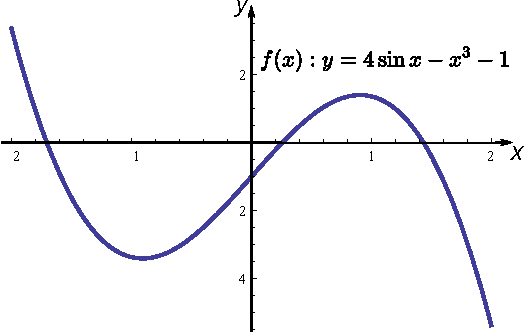
\includegraphics[scale=1]{fce_sinx.pdf}
           \captionof{figure}{Graf funkce $f(x):y=4\sin x - x^3 - 1$.}
           \label{nm:fig_ex_fce_sinx}
           \par}
        Z obrázku \ref{nm:fig_ex_fce_sinx} zjistíme, že existují tři kořeny: $x_1^*\in(-2,-1),
        x_2^*\in(-1, 0)$ a $x_3^*\in(1, 2)$.
      \end{example}
  
      Z obrázku zjistíme, že existují tři kořeny: $x_1^*\in(-2,-1),x_2^*\in(0,1),x_3^*\in(1,2)$.
      Zkusme najít kořeny v těchto intervalech pomocí numerických metod popsaných v následujících
      odstavcích
  
    \subsection{Metoda bisekce}
      Metoda známá také jako \textbf{metoda půlení intervalů}, je založena na principu
      zna\-mén\-ko\-vých změn. Předpokládejme, že funkce $f(x)$ má v koncových bodech intervalu
      $(a_0,b_0)$ opačná znaménka, tj. platí $f(a_0 )\cdot f(b_0 )<0$. Sestrojíme posloupnost
      intervalů $(a_1,b_1)\supset(a_2,b_2)\supset(a_3,b_3)\supset\cdots$, které obsahují kořen.
      Intervaly $(a_{k+1},b_{k+1}), k=0,1,\cdots$, určíme rekurzivně způsobem, který si nyní
      popíšeme.
  
      Střed intervalu $(a_k,b_k)$ je bod $x_{k+1}=\frac{1}{2}(a_k+b_k)$. Když $f(x_k)=0$, pak
      $x_{k+1}=x^*$ je kořen a dál nepokračujeme.

} %tikzset
%---------------------------------------------------------------------------------------------------
%\printbibliography[heading=subbibliography]
\addcontentsline{toc}{section}{Seznam literatury}
} % DEBUG was off